
%DIF LATEXDIFF DIFFERENCE FILE
%DIF DEL flattened.tex           Tue Oct  7 18:48:32 2025
%DIF ADD flattened_spelled.tex   Tue Oct  7 18:48:42 2025

\documentclass[12pt,a4paper,twoside,openright,final,titlepage]{report}
\usepackage[utf8]{inputenc}
\usepackage{layout}
\usepackage{lscape}
\usepackage{rotating}
\usepackage{longtable}
\usepackage{enumitem}
\usepackage{cite}
\usepackage{fixme}


\setlength{\headheight}{15pt}



\usepackage{setspace}
\usepackage{svg}
\onehalfspacing

\usepackage{fancyhdr}
\usepackage[T1]{fontenc}     \usepackage{lmodern}         

\usepackage[labelfont=bf]{caption}
\usepackage{enumitem}
\usepackage[utf8]{inputenc}
\usepackage[a4paper,width=150mm,top=25mm,bottom=25mm]{geometry}
\usepackage{tocbibind}
\usepackage[automake,acronym,toc]{glossaries-extra}

\usepackage{comment}
\usepackage[section]{placeins} \usepackage{graphicx}
\usepackage{multirow}
\usepackage{array}
\usepackage[hidelinks]{hyperref}[hyphens]
\usepackage[percent]{overpic}
\usepackage{xcolor}
\usepackage{pdfpages}

\newcommand{\nocontentsline}[3]{}
\let\origcontentsline\addcontentsline
\newcommand\stoptoc{\let\addcontentsline\nocontentsline}
\newcommand\resumetoc{\let\addcontentsline\origcontentsline}



\usepackage{cleveref}
\usepackage{chngcntr}

\usepackage{algorithm}
\usepackage{algpseudocode}
\usepackage{amsmath,amsfonts,amssymb,amsthm}

\makeatletter
\newcommand{\thickhline}{\noalign {\ifnum 0=`}\fi \hrule height 1pt
    \futurelet \reserved@a \@xhline
}

\newcolumntype{"}{!{\vrule width 1pt}}
\makeatother


\renewcommand{\chaptermark}[1]{\markboth{\MakeUppercase{\thechapter. #1 }}{}}
\renewcommand{\sectionmark}[1]{}
\counterwithin{algorithm}{section} \crefname{algorithm}{Algorithm}{Algorithms}

\fancyhf{}
\fancyhead[RO]{\bfseries\rightmark}
\fancyhead[LE]{\bfseries\leftmark}
\fancyfoot[C]{\thepage}
\pagestyle{fancy}

\usepackage[english]{babel}
\addto\extrasenglish{
  \def\subsectionautorefname{Subsection}
}
\addto\extrasenglish{
  \def\sectionautorefname{Section}
}
\addto\extrasenglish{
  \def\chapterautorefname{Chapter}
}

\newcommand\frontmatter{\pagenumbering{roman}}
\newcommand\mainmatter{\cleardoublepage\pagenumbering{arabic}}

\newenvironment{chapabstract}{\begin{center}\singlespacing
		\bfseries ABSTRACT
	\end{center}
    }


\makeglossaries
    
%DIF PREAMBLE EXTENSION ADDED BY LATEXDIFF
%DIF UNDERLINE PREAMBLE %DIF PREAMBLE
\RequirePackage[normalem]{ulem} %DIF PREAMBLE
\RequirePackage{color}\definecolor{RED}{rgb}{1,0,0}\definecolor{BLUE}{rgb}{0,0,1} %DIF PREAMBLE
\providecommand{\DIFaddtex}[1]{{\protect\color{blue}\uwave{#1}}} %DIF PREAMBLE
\providecommand{\DIFdeltex}[1]{{\protect\color{red}\sout{#1}}} %DIF PREAMBLE
%DIF SAFE PREAMBLE %DIF PREAMBLE
\providecommand{\DIFaddbegin}{} %DIF PREAMBLE
\providecommand{\DIFaddend}{} %DIF PREAMBLE
\providecommand{\DIFdelbegin}{} %DIF PREAMBLE
\providecommand{\DIFdelend}{} %DIF PREAMBLE
\providecommand{\DIFmodbegin}{} %DIF PREAMBLE
\providecommand{\DIFmodend}{} %DIF PREAMBLE
%DIF FLOATSAFE PREAMBLE %DIF PREAMBLE
\providecommand{\DIFaddFL}[1]{\DIFadd{#1}} %DIF PREAMBLE
\providecommand{\DIFdelFL}[1]{\DIFdel{#1}} %DIF PREAMBLE
\providecommand{\DIFaddbeginFL}{} %DIF PREAMBLE
\providecommand{\DIFaddendFL}{} %DIF PREAMBLE
\providecommand{\DIFdelbeginFL}{} %DIF PREAMBLE
\providecommand{\DIFdelendFL}{} %DIF PREAMBLE
%DIF HYPERREF PREAMBLE %DIF PREAMBLE
\providecommand{\DIFadd}[1]{\texorpdfstring{\DIFaddtex{#1}}{#1}} %DIF PREAMBLE
\providecommand{\DIFdel}[1]{\texorpdfstring{\DIFdeltex{#1}}{}} %DIF PREAMBLE
\newcommand{\DIFscaledelfig}{0.5}
%DIF HIGHLIGHTGRAPHICS PREAMBLE %DIF PREAMBLE
\RequirePackage{settobox} %DIF PREAMBLE
\RequirePackage{letltxmacro} %DIF PREAMBLE
\newsavebox{\DIFdelgraphicsbox} %DIF PREAMBLE
\newlength{\DIFdelgraphicswidth} %DIF PREAMBLE
\newlength{\DIFdelgraphicsheight} %DIF PREAMBLE
% store original definition of \includegraphics %DIF PREAMBLE
\LetLtxMacro{\DIFOincludegraphics}{\includegraphics} %DIF PREAMBLE
\newcommand{\DIFaddincludegraphics}[2][]{{\color{blue}\fbox{\DIFOincludegraphics[#1]{#2}}}} %DIF PREAMBLE
\newcommand{\DIFdelincludegraphics}[2][]{% %DIF PREAMBLE
\sbox{\DIFdelgraphicsbox}{\DIFOincludegraphics[#1]{#2}}% %DIF PREAMBLE
\settoboxwidth{\DIFdelgraphicswidth}{\DIFdelgraphicsbox} %DIF PREAMBLE
\settoboxtotalheight{\DIFdelgraphicsheight}{\DIFdelgraphicsbox} %DIF PREAMBLE
\scalebox{\DIFscaledelfig}{% %DIF PREAMBLE
\parbox[b]{\DIFdelgraphicswidth}{\usebox{\DIFdelgraphicsbox}\\[-\baselineskip] \rule{\DIFdelgraphicswidth}{0em}}\llap{\resizebox{\DIFdelgraphicswidth}{\DIFdelgraphicsheight}{% %DIF PREAMBLE
\setlength{\unitlength}{\DIFdelgraphicswidth}% %DIF PREAMBLE
\begin{picture}(1,1)% %DIF PREAMBLE
\thicklines\linethickness{2pt} %DIF PREAMBLE
{\color[rgb]{1,0,0}\put(0,0){\framebox(1,1){}}}% %DIF PREAMBLE
{\color[rgb]{1,0,0}\put(0,0){\line( 1,1){1}}}% %DIF PREAMBLE
{\color[rgb]{1,0,0}\put(0,1){\line(1,-1){1}}}% %DIF PREAMBLE
\end{picture}% %DIF PREAMBLE
}\hspace*{3pt}}} %DIF PREAMBLE
} %DIF PREAMBLE
\LetLtxMacro{\DIFOaddbegin}{\DIFaddbegin} %DIF PREAMBLE
\LetLtxMacro{\DIFOaddend}{\DIFaddend} %DIF PREAMBLE
\LetLtxMacro{\DIFOdelbegin}{\DIFdelbegin} %DIF PREAMBLE
\LetLtxMacro{\DIFOdelend}{\DIFdelend} %DIF PREAMBLE
\DeclareRobustCommand{\DIFaddbegin}{\DIFOaddbegin \let\includegraphics\DIFaddincludegraphics} %DIF PREAMBLE
\DeclareRobustCommand{\DIFaddend}{\DIFOaddend \let\includegraphics\DIFOincludegraphics} %DIF PREAMBLE
\DeclareRobustCommand{\DIFdelbegin}{\DIFOdelbegin \let\includegraphics\DIFdelincludegraphics} %DIF PREAMBLE
\DeclareRobustCommand{\DIFdelend}{\DIFOaddend \let\includegraphics\DIFOincludegraphics} %DIF PREAMBLE
\LetLtxMacro{\DIFOaddbeginFL}{\DIFaddbeginFL} %DIF PREAMBLE
\LetLtxMacro{\DIFOaddendFL}{\DIFaddendFL} %DIF PREAMBLE
\LetLtxMacro{\DIFOdelbeginFL}{\DIFdelbeginFL} %DIF PREAMBLE
\LetLtxMacro{\DIFOdelendFL}{\DIFdelendFL} %DIF PREAMBLE
\DeclareRobustCommand{\DIFaddbeginFL}{\DIFOaddbeginFL \let\includegraphics\DIFaddincludegraphics} %DIF PREAMBLE
\DeclareRobustCommand{\DIFaddendFL}{\DIFOaddendFL \let\includegraphics\DIFOincludegraphics} %DIF PREAMBLE
\DeclareRobustCommand{\DIFdelbeginFL}{\DIFOdelbeginFL \let\includegraphics\DIFdelincludegraphics} %DIF PREAMBLE
\DeclareRobustCommand{\DIFdelendFL}{\DIFOaddendFL \let\includegraphics\DIFOincludegraphics} %DIF PREAMBLE
%DIF AMSMATHULEM PREAMBLE %DIF PREAMBLE
\makeatletter %DIF PREAMBLE
\let\sout@orig\sout %DIF PREAMBLE
\renewcommand{\sout}[1]{\ifmmode\text{\sout@orig{\ensuremath{#1}}}\else\sout@orig{#1}\fi} %DIF PREAMBLE
\makeatother %DIF PREAMBLE
%DIF COLORLISTINGS PREAMBLE %DIF PREAMBLE
\RequirePackage{listings} %DIF PREAMBLE
\RequirePackage{color} %DIF PREAMBLE
\lstdefinelanguage{DIFcode}{ %DIF PREAMBLE
%DIF DIFCODE_UNDERLINE %DIF PREAMBLE
  moredelim=[il][\color{red}\sout]{\%DIF\ <\ }, %DIF PREAMBLE
  moredelim=[il][\color{blue}\uwave]{\%DIF\ >\ } %DIF PREAMBLE
} %DIF PREAMBLE
\lstdefinestyle{DIFverbatimstyle}{ %DIF PREAMBLE
	language=DIFcode, %DIF PREAMBLE
	basicstyle=\ttfamily, %DIF PREAMBLE
	columns=fullflexible, %DIF PREAMBLE
	keepspaces=true %DIF PREAMBLE
} %DIF PREAMBLE
\lstnewenvironment{DIFverbatim}{\lstset{style=DIFverbatimstyle}}{} %DIF PREAMBLE
\lstnewenvironment{DIFverbatim*}{\lstset{style=DIFverbatimstyle,showspaces=true}}{} %DIF PREAMBLE
\lstset{extendedchars=\true,inputencoding=utf8}

%DIF END PREAMBLE EXTENSION ADDED BY LATEXDIFF

\begin{document}

\newglossaryentry{SpaitalAwareness}
{
    name=Spatial awareness,
    plural=Spatial awarenesses,
    description={The ability to perceive and understand the spatial relationships between objects in the environment, as well as the position and movement of one's own body in relation to those objects. It is a fundamental aspect of human perception and is essential for many activities, such as navigation, manipulation of objects, and interaction with others.}
}

\newglossaryentry{Depth Perception}
{
    name=Depth Perception,
    plural=Depth Perceptions,
    description={The ability to perceive and judge the spatial relationships between objects in three dimensions. An essential aspect of human vision, allowing us to navigate and interact with the physical environment.}
}

\newglossaryentry{X-ray Visualization}
{
    name=X-ray Visualization,
    plural=X-ray Visualizations,
    description={A rendering or graphical technique used in computer graphics, medical imaging, and augmented reality to simulate the effect of looking through solid objects. Instead of physically penetrating materials as in real X-rays, this method selectively hides, fades, or highlights parts of a model or environment to reveal obscured internal structures or layers for analysis, learning, or interaction.}
}

\newglossaryentry{X-ray Vision}
{
    name=X-ray Vision,
    description={A perceptual or technological capability, either fictional or simulated, that allows an observer to see through opaque objects and reveal their hidden interior structures or the environment beyond them. In practice, X-ray vision is achieved through imaging technologies or visual effects that mimic this ability, providing insights not accessible through direct surface observation.}
}





\newglossaryentry{AugmentedRealityX-rayVision}
{
    name=Augmented Reality enabled X-ray Vision,
    plural=Augmented Reality enabled X-ray Visions,
    description={The ability to overlay virtual content on top of the real-world environment, allowing users to see virtual objects positioned behind real-world obstacles.}
}

\newglossaryentry{microsaccades}
{
    name=Microsaccades,
    text=microsaccades,
    description={Microsaccades are tiny, involuntary eye movements that occur even when we try to maintain fixation on a point, serving important functions in visual perception and attention by preventing sensory adaptation and aiding in gathering additional visual information from the environment.}
}

\newglossaryentry{ar_g}{
    name= {Augmented Reality},
    plural= {Augmented Reality},
    description={A technology that overlays digital information and virtual objects onto the real world, enhancing the user's perception and interaction with their environment through a smartphone or smart glasses device. By blending the physical and digital realms, AR provides immersive experiences and practical applications across various industries, ranging from entertainment and gaming to education and industrial design.}
}

\newglossaryentry{ar}{
    type=\acronymtype, 
    name = {AR\glsadd{ar_g}},
    description={Augmented Reality\glsadd{ar_g}}, 
    plural={AR},
    first={Augmented Reality (AR)\glsadd{ar_g}}, 
    see=[Glossary:]{ar_g}
}

\newglossaryentry{vr_g}{
name= {Virtual Reality},
plural={Virtual Reality},
description={A technology that creates a simulated and immersive digital environment, typically experienced through a head-mounted display and motion-tracking devices. It transports users to a computer-generated world, allowing them to interact with realistic or fantastical scenarios, offering a range of applications from entertainment and gaming to training and therapy.}
}

\newglossaryentry{vr}{
type=\acronymtype,
name = {VR},
plural = {VR},
description = {Virtual Reality},
first={Virtual Reality (VR)\glsadd{vr_g}},
see=[Glossary:]{vr_g}
}

\newglossaryentry{ost_g}{
name= {Ocular See Through},
plural = {Ocular See Through},
description={A technology that provides a transparent display, allowing users to view the real world while overlaying digital information or virtual objects onto their field of vision. By enabling the simultaneous perception of the physical and digital environments, OST enhances user experiences and finds applications in various fields, including gaming, navigation, and industrial training.}
}

\newglossaryentry{ost}{
type=\acronymtype,
name = {OST},
plural = {OST},
description={Ocular See Through},
first={Ocular See Through (OST)\glsadd{ost_g}},
see=[Glossary:]{ost_g}
}

\newglossaryentry{vst_g}{
name= {Video See Through},
plural= {Video See Through},
description={A technology that utilizes a video feed from cameras to overlay digital information or virtual objects onto the real world, allowing users to see their surroundings through a display device. By merging live video footage with computer-generated graphics, VST enhances user perception and enables interactive experiences in fields such as gaming, medical imaging, and remote assistance.}
}

\newglossaryentry{vst}{
type=\acronymtype,
name = {VST},
plural = {VST},
description={Video See Through},
first={Video See Through (VST)\glsadd{vst_g}},
see=[Glossary:]{vst_g}
}

\newglossaryentry{dvr_g}{
name= {Direct Volume Rendering},
plural={Direct Volume Rendering},
description={A technique in computer graphics and visualization that allows for the direct generation of images from volumetric data, such as medical scans or scientific simulations. DVR enables the exploration and visualization of complex three-dimensional structures and phenomena by applying various rendering algorithms and shading techniques.}
}

\newglossaryentry{dvr}{
type=\acronymtype,
name = {DVR},
plural = {DVR},
description={Direct Volume Rendering},
first={Direct Volume Rendering (DVR)\glsadd{dvr_g}},
see=[Glossary:]{dvr_g}
}

\newglossaryentry{lmm_g}{
name= {Linear Mixed Effects Models},
description={A statistical modeling approach that incorporates both fixed effects and random effects to analyze data with hierarchical or clustered structures. LMMs are used to account for within-group dependencies and capture individual variations, making them suitable for studying longitudinal or repeated measures data in various fields, including social sciences, biology, and psychology.}
}

\newglossaryentry{lmm}{
type=\acronymtype,
name = {LMM},
plural = {LMMs},
description={Linear Mixed Effects Models},
first={Linear Mixed Effects Models (LMM)\glsadd{lmm_g}},
see=[Glossary:]{lmm_g}
}

\newglossaryentry{hsd}{
    type=\acronymtype,
    name = {HSD},
    plural = {HSD},
    description={Honestly Significant Difference},
    first={Honestly Significant Difference (HSD)}
}

\newglossaryentry{hmd_g}{
name= {Head Mounted Device},
description={Technological devices that are worn on the head and typically feature a display screen, enabling users to experience immersive visual and auditory content. Head Mounted Devices, such as virtual reality headsets or augmented reality glasses, provide a user-centric interface and are widely used for gaming, virtual simulations, training, and entertainment purposes.}
}

\newglossaryentry{hmd}{
type=\acronymtype,
name = {HMD},
plural = {HMDs},
description={Head Mounted Device},
first={Head Mounted Device (HMD)\glsadd{hmd_g}},
firstplural={Head-Mounted Displays (HMDs)\glsadd{hmd_g}}
see=[Glossary:]{hmd_g}
}

\newglossaryentry{ct_g}{
    name= {Computed Tomography},
    plural= {Computed Tomographies},
    description={A medical imaging technique that uses X-ray technology to create detailed cross-sectional images of the body. Computed Tomography (CT) scans provide valuable diagnostic information by capturing multiple X-ray images from different angles and combining them to generate a three-dimensional representation. CT scans are commonly used to diagnose various conditions and guide medical procedures.}
}

\newglossaryentry{ct}{
    type=\acronymtype,
    name = {CT},
    plural = {CTs},
    description={Computed Tomography},
    first={Computed Tomography (CT)\glsadd{ct_g}},
    firstplural={Computed Tomographies (CTs)\glsadd{ct_g}},
    see=[Glossary:]{ct_g}
}

\newglossaryentry{mri_g}{
    name= {Magnetic Resonance Imaging},
    plural={Magnetic Resonance Imagings},
    description={A medical imaging technique that uses strong magnetic fields and radio waves to create detailed images of the internal structures of the body. Magnetic Resonance Imaging (MRI) provides high-resolution images that help diagnose various conditions and assess the health of organs and tissues. MRI scans are widely used in medicine for their non-invasive nature and ability to visualize soft tissues with excellent contrast.}
}

\newglossaryentry{mri}{
    type=\acronymtype,
    name = {MRI},
    plural = {MRIs},
    description={Magnetic Resonance Imaging},
    first={Magnetic Resonance Imaging (MRI)\glsadd{mri_g}},
    firstplural={Magnetic Resonance Imagings (MRIs)\glsadd{mri_g}},
    see=[Glossary:]{mri_g}
}

\newglossaryentry{sus_g}{
    name= {System Usability Scale},
    plural={System Usability Scales},
    description={A widely used questionnaire-based method for assessing the usability of a system or product. The System Usability Scale (SUS) consists of a set of standardized statements and Likert scale responses that provide quantitative measures of perceived usability, effectiveness, and user satisfaction. SUS scores are commonly used in user experience research to evaluate and compare the usability of different systems or product designs.}
}

\newglossaryentry{sus}{
    type=\acronymtype,
    name = {SUS},
    plural = {SUS},
    description={System Usability Scale},
    first={System Usability Scale (SUS)\glsadd{sus_g}},
    firstplural={System Usability Scales (SUS)\glsadd{sus_g}},
    see=[Glossary:]{sus_g}
}

\newglossaryentry{sar_g}{
    name= {Spatial Augmented Reality},
    plural={Spatial Augmented Realities},
    description={A technology that enhances the physical environment by projecting digital content onto real-world surfaces, such as walls, floors, or objects. Spatial Augmented Reality (SAR) combines projection mapping techniques with computer vision and spatial tracking to create interactive and immersive experiences. SAR finds applications in areas such as art installations, architectural visualization, and interactive displays.}
}

\newglossaryentry{sar}{
    type=\acronymtype,
    name = {SAR},
    plural = {SAR},
    description={Spatial Augmented Reality},
    first={Spatial Augmented Reality (SAR)\glsadd{sar_g}},
    firstplural={Spatial Augmented Realities (SAR)\glsadd{sar_g}},
    see=[Glossary:]{sar_g}
}

\newglossaryentry{imu_g}{
    name= {Inertial Measurement Unit},
    plural={Inertial Measurement Units},
    description={A sensor module that combines multiple inertial sensors, such as accelerometers, gyroscopes, and magnetometers, to measure and track an object's motion and orientation in real time. Inertial Measurement Units (IMUs) are commonly used in applications that require motion sensing, such as robotics, virtual reality, and motion capture systems. IMUs provide essential data for estimating objects' position, velocity, and orientation changes.}
}

\newglossaryentry{imu}{
    type=\acronymtype,
    name = {IMU},
    plural = {IMUs},
    description={Inertial Measurement Unit},
    first={Inertial Measurement Unit (IMU)\glsadd{imu_g}},
    firstplural={Inertial Measurement Units (IMUs)\glsadd{imu_g}},
    see=[Glossary:]{imu_g}
}

\newglossaryentry{dicom_g}{
    name= {Digital Imaging and Communications in Medicine},
    plural={Digital Imaging and Communications in Medicines},
    description={A standard for managing, storing, and transmitting medical images and related data. DICOM (Digital Imaging and Communications in Medicine) enables interoperability between different medical imaging devices and systems, ensuring compatibility and consistent communication of medical information. It is widely used in healthcare settings to store and exchange medical images, such as X-rays, CT scans, and MRIs.}
}

\newglossaryentry{dicom}{
    type=\acronymtype,
    name = {DICOM},
    plural = {DICOM},
    description={Digital Imaging and Communications in Medicine},
    first={Digital Imaging and Communications in Medicine (DICOM)\glsadd{dicom_g}},
    firstplural={Digital Imaging and Communications in Medicines (DICOM)\glsadd{dicom_g}},
    see=[Glossary:]{dicom_g}
}

\newglossaryentry{pc_g}{
    name= {Personal Computer},
    plural={Personal Computers},
    description={A type of computer designed for individual use, typically consisting of a central processing unit (CPU), memory, storage, and input/output devices. Personal computers (PCs) are widely used for various purposes, including work, communication, entertainment, and personal productivity. They offer a flexible and customizable computing platform for users to perform tasks, run software applications, and access the internet.}
}

\newglossaryentry{pc}{
    type=\acronymtype,
    name = {PC},
    plural = {PCs},
    description={Personal Computer},
    first={Personal Computer (PC)\glsadd{pc_g}},
    firstplural={Personal Computers (PCs)\glsadd{pc_g}},
    see=[Glossary:]{pc_g}
}

\newglossaryentry{hu_g}{
    name= {Hounsfield Units},
    plural={Hounsfield Units},
    description={A unit of measurement used in computed tomography (CT) imaging to quantify the radiodensity of tissues. Hounsfield Units (HU) assign a numerical value to tissue attenuation, where higher values represent denser or more radio-opaque structures and lower values indicate less dense or more radio-lucent structures. HU values help in differentiating and characterizing various tissues and abnormalities in medical imaging.}
}

\newglossaryentry{hu}{
    type=\acronymtype,
    name = {HU},
    plural = {HU},
    description={Hounsfield Units},
    first={Hounsfield Units (HU)\glsadd{hu_g}},
    firstplural={Hounsfield Units (HU)\glsadd{hu_g}},
    see=[Glossary:]{hu_g}
}

\newglossaryentry{mr_g}{
    name= {Mixed Reality},
    plural={Mixed Realities},
    description={A technology that merges elements of both the physical and virtual worlds, creating a seamless and interactive environment. Mixed Reality combines aspects of both Augmented Reality (AR) and Virtual Reality (VR), allowing users to interact with digital objects while maintaining awareness of the real world. This technology finds applications in fields such as gaming, architecture, training, and collaborative workspaces.}
}

\newglossaryentry{mr}{
    type=\acronymtype,
    name = {MR},
    plural = {MR},
    description={Mixed Reality},
    first={Mixed Reality (MR)\glsadd{mr_g}},
    firstplural={Mixed Realities (MR)\glsadd{mr_g}},
    see=[Glossary:]{mr_g}
}

\newglossaryentry{caves_g}{
    name= {Cave Automatic Virtual Environment},
    plural={Cave Automatic Virtual Environments},
    description={Cave Automatic Virtual Environment, or CAVE, is an immersive virtual reality environment that utilizes multiple large displays and surround sound to create a fully immersive experience. Users typically stand within a room-sized cube, and the walls, floor, and ceiling are used as screens to display virtual content. A CAVE provides a highly immersive and interactive virtual reality experience, enabling users to navigate and interact with digital environments naturally and intuitively. It finds applications in fields such as scientific visualization, architectural design, and medical research.}
}



\newglossaryentry{cave}{
    type=\acronymtype, 
    name = {CAVE},
    plural = {CAVEs},
    description={Cave Automatic Virtual Environment}, 
    first={Cave Automatic Virtual Environment (CAVE)\glsadd{caves_g}}, 
    firstplural={Cave Automatic Virtual Environments (CAVEs)\glsadd{caves_g}},
    see=[Glossary:]{caves_g}
}

\newglossaryentry{ultrasound}{
    name= {Ultrasound},
    plural={Ultrasounds},
    text= {ultrasound},
    description={A medical imaging technique that uses high-frequency sound waves to visualize internal structures of the body. Ultrasound imaging, also known as sonography, produces real-time images by emitting sound waves and capturing their reflections off tissues and organs. It is commonly used for non-invasive imaging of various body parts, such as the abdomen, heart, and developing fetus, and plays a crucial role in diagnosing medical conditions.}
}

\newglossaryentry{xray}{
    name= {X-ray},
    plural={X-rays},
    description={A form of electromagnetic radiation commonly used in medical imaging to visualize the body's internal structures. X-ray imaging involves passing X-ray photons through the body, with denser tissues absorbing more photons, resulting in varying levels of brightness in the final image. X-rays are widely utilized for diagnosing bone fractures, detecting abnormalities, and examining structures like the chest, teeth, and bones.}
}

\newglossaryentry{gantry}{
    name= {Gantry},
    plural={Gantries},
    text= {gantry},
    description={The circular or cylindrical structure of a CT scanner that houses the X-ray tube and detector array. The gantry rotates around the patient during the scanning process, capturing X-ray images from various angles. It plays a crucial role in producing cross-sectional images of the body, which are then used to reconstruct detailed 3D images. The design of the gantry allows for precise positioning and accurate imaging during CT scans.}
}

\newglossaryentry{isosurface}{
    name= {Iso-surface},
    plural={Iso-surfaces},
    text= {iso-surface},
    description={A three-dimensional representation of a specific value or range within a volumetric dataset, often used in scientific visualization. An iso-surface is created by identifying voxels (3D pixels) within the dataset that match a certain threshold value and then rendering the surface that connects these voxels. Iso-surfaces are useful for visualizing structures and boundaries within complex datasets, such as medical imaging scans or simulations in various scientific fields.}
}

\newglossaryentry{pathology}{
    name= {Pathology},
    plural={Pathologies},
    text= {pathology},
    description={The medical specialty that involves the study and diagnosis of diseases by examining tissue samples, cells, and bodily fluids. Pathologists analyze the structural and functional changes in tissues and organs to understand the nature of diseases and their underlying causes. Pathology plays a crucial role in disease diagnosis, treatment planning, and research, contributing to advancements in medical knowledge and patient care.}
}

\newglossaryentry{pathological}{
    name= {Pathological},
    plural={Pathologicals},
    text= {pathological},
    description={Relating to the study of diseases or disorders in living organisms. Pathological conditions involve abnormal changes in structure or function that can lead to health issues. Pathological studies aim to understand diseases' causes, mechanisms, and effects, often involving laboratory analysis, imaging, and clinical observations.}
    see=[Glossary:]{pathology}
}

\newglossaryentry{ui_g}{
    name= {User Interface},
    plural={User Interfaces},
    description={The point of interaction between a user and a digital or mechanical device, system, or software application. User interfaces encompass visual, auditory, and tactile elements that allow users to interact with and control devices or software, making it easier for humans to operate and communicate with machines. Effective user interfaces are crucial for ensuring a positive user experience and optimizing usability.}
}

\newglossaryentry{ui}{
    type=\acronymtype, 
    name = {UI},
    plural = {UIs},
    description={User Interface}, 
    first={User Interface (UI)\glsadd{ui_g}}, 
    firstplural={User Interfaces (UIs)\glsadd{ui_g}},
    see=[Glossary:]{ui_g}
}

\newglossaryentry{gui_g}{
    name= {Graphical User Interface},
    plural={Graphical User Interfaces},
    description={A type of user interface that allows users to interact with a computer or software application through graphical elements such as icons, buttons, windows, and menus. Graphical User Interfaces make it easier for users to perform tasks and access functions by providing visual representations of actions and options. GUIs are commonly used in operating systems, software applications, and websites, enhancing user accessibility and usability.}
}

\newglossaryentry{gui}{
    type=\acronymtype, 
    name = {GUI},
    plural = {GUIs},
    description={Graphical User Interface}, 
    first={Graphical User Interface (GUI)\glsadd{gui_g}}, 
    firstplural={Graphical User Interfaces (GUIs)\glsadd{gui_g}},
    see=[Glossary:]{gui_g}
}

\newglossaryentry{ai_g}{
    name= {Artificial Intelligence},
    plural={Artificial Intelligences},
    description={A branch of computer science that focuses on creating intelligent machines capable of performing tasks that typically require human intelligence. Artificial Intelligence (AI) involves developing algorithms and models that enable computers to process data, learn from it, and make decisions or predictions. AI finds applications in a wide range of fields, including natural language processing, machine learning, robotics, and data analysis, revolutionizing industries and enhancing automation and problem-solving capabilities.}
}

\newglossaryentry{ai}{
    type=\acronymtype, 
    name = {AI},
    plural = {AI},
    description={Artificial Intelligence}, 
    first={Artificial Intelligence (AI)\glsadd{ai_g}}, 
    firstplural={Artificial Intelligences (AI)\glsadd{ai_g}},
    see=[Glossary:]{ai_g}
}

\newglossaryentry{rd_g}{
    name= {Research and Development},
    plural={Research and Developments},
    description={The process of systematically investigating, designing, and creating new products, technologies, or processes, as well as improving existing ones. Research and Development (R\&D) activities aim to enhance knowledge and capabilities, leading to innovation and advancements in various fields, including science, technology, and industry. R\&D plays a critical role in driving economic growth, competitiveness, and the development of cutting-edge solutions across sectors.}
}

\newglossaryentry{rd}{
    type=\acronymtype, 
    name = {R\&D},
    plural = {R\&D},
    description={Research and Development}, 
    first={Research and Development (R\&D)\glsadd{rd_g}}, 
    firstplural={Research and Developments (R\&D)\glsadd{rd_g}},
    see=[Glossary:]{rd_g}
}

\newglossaryentry{ctc_g}{
    name= {Circulating Tumor Cells},
    plural={Circulating Tumor Cells},
    description={Tumor cells that have detached from the primary tumor and entered the bloodstream or lymphatic system, allowing them to circulate throughout the body. Circulating Tumor Cells (CTCs) can provide valuable information about cancer progression, metastasis, and treatment effectiveness through a simple blood test. The detection and analysis of CTCs have implications for cancer diagnosis, treatment planning, and monitoring patient response to therapy.}
}

\newglossaryentry{ctc}{
    type=\acronymtype, 
    name = {CTC},
    plural = {CTCs},
    description={Circulating Tumor Cells}, 
    first={Circulating Tumor Cells (CTC)\glsadd{ctc_g}}, 
    firstplural={Circulating Tumor Cells (CTCs)\glsadd{ctc_g}},
    see=[Glossary:]{ctc_g}
}

\newglossaryentry{di_g}{
    name= {Digital Imaging},
    plural={Digital Imagings},
    description={The process of capturing, storing, and displaying visual information in digital format, allowing for the manipulation, analysis, and transmission of images using electronic devices and computer systems. Digital Imaging has transformed fields such as photography, medical imaging, and remote sensing, offering improved image quality, storage efficiency, and the ability to apply various image processing techniques. It plays a vital role in diverse applications, including healthcare, entertainment, and scientific research.}
}

\newglossaryentry{di}{
    type=\acronymtype, 
    name = {DI},
    plural = {DI},
    description={Digital Imaging}, 
    first={Digital Imaging (DI)\glsadd{di_g}}, 
    firstplural={Digital Imagings (DI)\glsadd{di_g}},
    see=[Glossary:]{di_g}
}

\newglossaryentry{shs_g}{
    name= {School of Health Sciences},
    plural={Schools of Health Sciences},
    description={An academic institution or department dedicated to the study and training of healthcare professionals in various disciplines, including medicine, nursing, pharmacy, and allied health fields. The School of Health Sciences (SHS) plays a crucial role in preparing students for careers in healthcare, research, and patient care, contributing to the advancement of medical knowledge and the improvement of healthcare services.}
}

\newglossaryentry{shs}{
    type=\acronymtype, 
    name = {SHS},
    plural = {SHS},
    description={School of Health Sciences}, 
    first={School of Health Sciences (SHS)\glsadd{shs_g}}, 
    firstplural={Schools of Health Sciences (SHS)\glsadd{shs_g}},
    see=[Glossary:]{shs_g}
}

\newglossaryentry{tesla_g}{
    name= {Tesla},
    plural={Teslas},
    description={A unit of measurement for the magnetic field strength used in Magnetic Resonance Imaging (MRI). The Tesla is the standard international unit, representing the strength of the magnetic field influencing the behavior of atomic nuclei during the imaging process. Higher Tesla values often contribute to improved image resolution and quality in MRI, impacting diagnostic capabilities in medical imaging.}
}

\newglossaryentry{tesla}{
    type=\acronymtype, 
    name = {T},
    plural = {T},
    description={Tesla}, 
    first={Tesla (T)\glsadd{tesla_g}}, 
    firstplural={Teslas (T)\glsadd{tesla_g}},
    see=[Glossary:]{tesla_g}
}





\newglossaryentry{pathologist}{
    name= {Pathologist},
    plural={Pathologists},
    text= {pathologist},
    description={A medical professional who specializes in the study and diagnosis of diseases. Pathologists analyze tissues, cells, and bodily fluids to understand the nature and causes of illnesses. Their expertise is crucial in providing accurate diagnoses, guiding treatment decisions, and contributing to medical research.}
}

\newglossaryentry{gpr_g}{
    name= {Ground Penetrating Radar},
    plural={Ground Penetrating Radars},
    description={A geophysical method that uses radar pulses to image the subsurface. Ground Penetrating Radar (GPR) is employed for detecting and mapping features underground, such as utilities, archaeological artifacts, and geological structures. It plays a crucial role in various fields, including civil engineering, environmental assessment, and archaeological exploration.}
}

\newglossaryentry{gpr}{
    type=\acronymtype, 
    name = {GPR},
    plural = {GPR},
    description={Ground Penetrating Radar}, 
    first={Ground Penetrating Radar (GPR)\glsadd{gpr_g}}, 
    firstplural={Ground Penetrating Radars (GPR)\glsadd{gpr_g}},
    see=[Glossary:]{gpr_g}
}

\newglossaryentry{gpu_g}{
    name= {Graphics Processing Unit},
    plural={Graphics Processing Units},
    description={A specialized electronic circuit designed to accelerate the processing of images and videos for display on a computer screen. Graphics Processing Units (GPUs) are essential components in rendering realistic graphics for applications such as gaming, video editing, and complex simulations. Their parallel processing capabilities make them well-suited for handling large-scale graphical computations.}
}

\newglossaryentry{gpu}{
    type=\acronymtype, 
    name = {GPU},
    plural = {GPUs},
    description={Graphics Processing Unit}, 
    first={Graphics Processing Unit (GPU)\glsadd{gpu_g}}, 
    firstplural={Graphics Processing Units (GPUs)\glsadd{gpu_g}},
    see=[Glossary:]{gpu_g}
}

\newglossaryentry{fps_g}{
    name= {Frames Per Second},
    plural={Frames Per Second},
    description={A metric that measures the number of individual frames or images displayed in one second. In the context of digital displays, including augmented reality, a higher frame rate, measured in frames per second (FPS), contributes to smoother and more fluid visual experiences. Higher FPS is particularly important in applications such as gaming and video playback.}
}

\newglossaryentry{fps}{
    type=\acronymtype, 
    name = {FPS},
    plural = {FPS},
    description={Frames Per Second}, 
    first={Frames Per Second (FPS)\glsadd{fps_g}}, 
    firstplural={Frames Per Second (FPS)\glsadd{fps_g}},
    see=[Glossary:]{fps_g}
}

\newglossaryentry{sql_g}{
    name= {Structured Query Language},
    plural={Structured Query Languages},
    description={A domain-specific language used for managing and manipulating relational databases. Structured Query Language (SQL) provides a standardized way to interact with databases, enabling tasks such as data querying, insertion, updating, and deletion. SQL is widely employed in software development, data analysis, and database management systems.}
}

\newglossaryentry{sql}{
    type=\acronymtype, 
    name = {SQL},
    plural = {SQL},
    description={Structured Query Language}, 
    first={Structured Query Language (SQL)\glsadd{sql_g}}, 
    firstplural={Structured Query Languages (SQL)\glsadd{sql_g}},
    see=[Glossary:]{sql_g}
}

\newglossaryentry{gan_g}{
    name= {Generative Adversarial Nets},
    plural={Generative Adversarial Nets},
    description={A class of artificial intelligence algorithms introduced by Ian Goodfellow and his colleagues in 2014. Generative Adversarial Nets (GANs) consist of two neural networks, a generator, and a discriminator, which are trained simultaneously through adversarial training. GANs are widely used for generating realistic synthetic data, image-to-image translation, style transfer, and other tasks in the realm of artificial intelligence and machine learning.}
}

\newglossaryentry{gan}{
    type=\acronymtype, 
    name = {GAN},
    plural = {GANs},
    description={Generative Adversarial Nets}, 
    first={Generative Adversarial Nets (GAN)\glsadd{gan_g}}, 
    firstplural={Generative Adversarial Nets (GANs)\glsadd{gan_g}},
    see=[Glossary:]{gan_g}
}

\newglossaryentry{virt}{
    type=\acronymtype, 
    name = {VIRT},
    plural = {VIRTs},
    description={Volumetric Illustrative Rendering Techniques}, 
    first={Volumetric Illustrative Rendering Techniques (VIRT)}
}

\newglossaryentry{sdf_g}{
    name= {Sign Distance Field},
    plural={Sign Distance Fields},
    description={A mathematical representation used in computer graphics to define the distance from a point in space to the nearest surface of an object. Sign Distance Fields (SDFs) are commonly employed in rendering techniques such as ray marching and distance field rendering. They allow for efficient and accurate rendering of complex shapes and can be used in various applications, including augmented reality, computer-aided design, and video games.}
}

\newglossaryentry{sdf}{
    type=\acronymtype, 
    name = {SDF},
    plural = {SDFs},
    description={Sign Distance Field}, 
    first={Sign Distance Field (SDF)\glsadd{sdf_g}}, 
    firstplural={Sign Distance Fields (SDFs)\glsadd{sdf_g}},
    see=[Glossary:]{sdf_g}
}

\newglossaryentry{aabb_g}{
    name= {Axis Aligned Bounding Box},
    plural={Axis Aligned Bounding Boxes},
    description={A rectangular cuboid aligned with the coordinate axes, typically used in computer graphics and computational geometry to enclose a set of objects or to define the spatial extent of an entity. Axis Aligned Bounding Boxes (AABBs) are commonly employed in collision detection algorithms, rendering optimizations, and spatial partitioning techniques. They provide a simple and efficient way to approximate the geometry of complex shapes and facilitate various operations in virtual environments, including augmented reality applications.}
}

\newglossaryentry{aabb}{
    type=\acronymtype, 
    name = {AABB},
    plural = {AABBs},
    description={Axis Aligned Bounding Box}, 
    first={Axis Aligned Bounding Box (AABB)\glsadd{aabb_g}}, 
    firstplural={Axis Aligned Bounding Boxes (AABBs)\glsadd{aabb_g}},
    see=[Glossary:]{aabb_g}
}

\newglossaryentry{hci_g}{
    name= {Human-Computer Interaction},
    plural={Human-Computer Interactions},
    description={A field of study focusing on the design and use of computer technology, particularly the interactions between humans (the users) and computers. HCI is concerned with the ways humans interact with computers and design technologies that let humans interact with computers in novel ways. It involves the study of how people use technology, the design of user-friendly interfaces, and the development of new interaction techniques to improve the user experience.}
}

\newglossaryentry{hci}{
    type=\acronymtype, 
    name = {HCI},
    plural = {HCI},
    description={Human-Computer Interaction}, 
    first={Human-Computer Interaction (HCI)\glsadd{hci_g}}, 
    firstplural={Human-Computer Interactions (HCI)\glsadd{hci_g}},
    see=[Glossary:]{hci_g}
}

\newglossaryentry{jnd_g}{
    name= {Just Noticeable Difference},
    plural={Just Noticeable Differences},
    description={The smallest change in a stimulus that can be detected by an observer, typically defined as the threshold at which a difference becomes perceptible to a human sensory system. In the context of visual perception, the Just Noticeable Difference (JND) refers to the minimum change in brightness, color, or other visual attribute that can be perceived by the human eye. Understanding JND is crucial in various fields, including image processing, display technology, and user interface design, to ensure optimal user experiences and minimize perceptual errors.}
}

\newglossaryentry{jnd}{
    type=\acronymtype, 
    name = {JND},
    plural = {JND},
    description={Just Noticeable Difference}, 
    first={Just Noticeable Difference (JND)\glsadd{jnd_g}}, 
    firstplural={Just Noticeable Differences (JND)\glsadd{jnd_g}},
    see=[Glossary:]{jnd_g}
}

\newglossaryentry{pse_g}{
    name= {Point of Subject Equality},
    plural={Points of Subject Equality},
    description={In psychophysics, the Point of Subject Equality (PSE) refers to the stimulus intensity at which a subject perceives two stimuli as being equal in some specific aspect, such as brightness, loudness, or size. It is a key concept used to study perceptual phenomena and understand the relationship between physical stimuli and subjective perception. The determination of PSE plays a crucial role in various fields, including sensory research, human factors engineering, and user experience design.}
}

\newglossaryentry{slam_g}{
    name= {Simultaneous Localization and Mapping},
    plural={Simultaneous Localizations and Mappings},
    description={Simultaneous Localization and Mapping (SLAM) is a technique used in robotics and computer vision to construct a map of an unknown environment while simultaneously tracking the position of the observer within that environment. SLAM systems utilize sensor data, such as camera images or laser scans, to estimate the robot's trajectory and create a map of its surroundings. This technology is essential for autonomous navigation in various applications, including self-driving cars, drones, and mobile robots.}
}

\newglossaryentry{slam}{
    type=\acronymtype, 
    name = {SLAM},
    plural = {SLAM},
    description={Simultaneous Localization and Mapping}, 
    first={Simultaneous Localization and Mapping (SLAM)\glsadd{slam_g}}, 
    firstplural={Simultaneous Localizations and Mappings (SLAM)\glsadd{slam_g}},
    see=[Glossary:]{slam_g}
}

\newglossaryentry{pse}{
    type=\acronymtype, 
    name = {PSE},
    plural = {PSE},
    description={Point of Subject Equality}, 
    first={Point of Subject Equality (PSE)\glsadd{pse_g}}, 
    firstplural={Points of Subject Equality (PSE)\glsadd{pse_g}},
    see=[Glossary:]{pse_g}
}

\newglossaryentry{twofc_g}{
    name= {Two-alternative forced choice},
    plural={Two-alternative forced choices},
    description={Two-alternative forced choice (2AFC) is a psychophysical method used to measure the detectability or discriminability of a stimulus. In a 2AFC task, the observer is presented with two alternatives and must choose which one matches the target stimulus or is different from a reference stimulus. This method is commonly used in perceptual experiments to assess sensory thresholds and performance in various domains, such as vision, audition, and touch.}
}

\newglossaryentry{twofc}{
    type=\acronymtype, 
    name = {2AFC},
    plural = {2AFC},
    description={Two-alternative forced choice}, 
    first={Two-alternative forced choice (2AFC)\glsadd{twofc_g}}, 
    firstplural={Two-alternative forced choices (2AFC)\glsadd{twofc_g}},
    see=[Glossary:]{twofc_g}
}

\newglossaryentry{regression_analysis}{
    name= {Regression Analysis},
    plural={Regression Analyses},
    description={A statistical method used to examine the relationship between one dependent variable and one or more independent variables. The goal of regression analysis is to model the expected value of the dependent variable in terms of the independent variables, allowing for prediction and understanding of the underlying patterns. It is widely used in fields such as economics, biology, engineering, and social sciences.}
}


\newglossaryentry{classifier_g}{
    name= {Classifier},
    plural={Classifiers},
    description={A classifier is an algorithm in machine learning and statistics used to assign categories or labels to data points based on input features. It operates by learning patterns from labeled training data and then predicting the categories of new, unseen data. Classifiers are used in various applications such as image recognition, spam detection, medical diagnosis, and more.}
}

\newglossaryentry{non_euclidean_space}{
    name= {Non-Euclidean Space},
    plural={Non-Euclidean Spaces},
    description={A type of geometric space that is not based on the postulates of Euclidean geometry. In non-Euclidean space, the parallel postulate of Euclidean geometry does not hold, leading to the development of hyperbolic and elliptic geometries. These spaces have unique properties and are used in various fields, including physics, computer science, and cosmology, to model complex structures and phenomena.}
}

\newglossaryentry{perspective_corrected_projection}{
    name= {Perspective-Corrected Projection},
    plural={Perspective-Corrected Projections},
    description={A technique used in computer graphics to ensure that textures and objects are rendered accurately from the viewer's perspective. This method corrects distortions that can occur in standard projections, providing a more realistic and visually consistent representation of 3D objects on a 2D screen. Perspective-corrected projection is essential for applications such as virtual reality, gaming, and simulations to enhance the immersive experience and maintain visual fidelity.}
}

\newglossaryentry{exocentric_perception}{
    name= {Exocentric Perception},
    plural={Exocentric Perceptions},
    first={exocentric}, 
    description={A perspective in which an observer views the environment from an external viewpoint, as if looking at a scene from outside their own body. This contrasts with egocentric perception, where the observer's viewpoint is from within their own body. Exocentric perception is commonly used in virtual reality and other visualization technologies to provide a broader, more comprehensive understanding of spatial relationships and object interactions within an environment.}
}

\newglossaryentry{ordinal_perception}{
    name= {Ordinal Perception},
    plural={Ordinal Perceptions},
    first={ordinal},
    description={The ability to perceive and understand the relative order or ranking of objects or events without necessarily quantifying the differences between them. In visual perception, this often involves recognizing that one object is in front of another or that one event occurred before another. Ordinal perception is crucial for tasks that require an understanding of sequences and hierarchies.}
}

\newglossaryentry{bfs_g}{
    name= {Breadth-First Search},
    plural={Breadth-First Searches},
    description={An algorithm for traversing or searching tree or graph data structures. It starts at the root (or an arbitrary node) and explores all nodes at the present depth level before moving on to nodes at the next depth level. BFS is commonly used in shortest path problems in unweighted graphs, level-order traversal of a tree, and in scenarios where we need to explore all nodes at the same distance from the starting node.}
}

\newglossaryentry{bfs}{
    type=\acronymtype, 
    name = {BFS},
    plural = {BFS},
    description={Breadth-First Search}, 
    first={Breadth-First Search (BFS)\glsadd{bfs_g}}, 
    firstplural={Breadth-First Searches (BFS)\glsadd{bfs_g}},
    see=[Glossary:]{bfs_g}
}

\newglossaryentry{voxel_g}{
    name= {Voxel},
    plural={Voxels},
    text= {voxel},
    description={A volumetric pixel, or voxel, represents a value on a regular grid in three-dimensional space. Voxels are commonly used in 3D graphics, medical imaging, and scientific simulations to model spatial data, enabling efficient rendering and analysis of complex structures. Unlike traditional 2D pixels, voxels contain depth information, making them essential for volumetric rendering and spatial partitioning.}
}

\newcommand{\newglossaryentrywithacronym}[3]{
\newglossaryentry{#1_gls}{
        name={#1},
        long={#2},
        description={#3}
    }

\newglossaryentry{#1}{
        type=\acronymtype,
        name={#1},
        description={#2},
        first={#2 (#1)\glsadd{#1_gls}},
        see=[Glossary:]{#1_gls}
    }
}

 \begin{titlepage}
		\centering
		\vfill
		\vskip 1.75cm
		{\bfseries\Large






        VIRTs: Volumetric Illustrative Rendering Techniques to Improve X-Ray Vision Perception on Optical See Through Mixed Reality

}
		\vskip 1.5cm

		\LARGE{Thomas John Clarke}\\
        \textit{\small BSoftwEng(Hons)}\\
        \LARGE

		\vskip 2.25cm	
            \large
		\textit{A dissertation presented for the degree of\\DOCTOR OF PHILOSOPHY}\\
		\vskip .05cm
		\includegraphics[width=.40\linewidth]{unisaLogo.jpg}
		\vskip .05cm
		Australian Research Centre for Interactive\\and Virtual Environments\\
		\vskip .25cm
		  March 2025\\
		\vskip 1.5cm
		\textbf{Supervisors:} \\
			A. Prof. Ross Smith (Coordinating)\\
			A. Prof. Wolfgang Mayer\\
			Dr. Joanne Zucco\\
	\end{titlepage}
\frontmatter
\clearpage
	\thispagestyle{empty}
	\phantom{a}
	\vfill
	\vfill


        \Huge
	\begin{abstract}
        \normalsize

    
Seeing through objects is a desirable trait not just for superheroes trying to escape from a burning building or locate a villain but for any professional who needs to consider what they cannot yet see. 
            This can be related to a construction worker who needs to know what is going on the floor above them or a surgeon who needs to know where an object is within the human body. 


            \gls{ar} X-ray vision can extend a userΓÇÖs sight into concealed spaces and through virtual objects to reveal hidden areas in the real world.
            However, this functionality hasn't been well explored using Optical See-Through (OST) Augmented Reality (AR). 
            OST AR devices allow users to perceive both the real world and digital overlays, enhancing their value for context switching between tasks that require virtual and real-world information. 
The ability to see the real world and the digital overlay simultaneously makes occlusion difficult, which is further impacted by the limited color \DIFdelbegin \DIFdel{gambut }\DIFdelend \DIFaddbegin \DIFadd{gamut }\DIFaddend of current OST AR displays, impacting colors like darker colors and blacks the worse. 
            This is all because the OST AR display utilizes a projector, which projects light onto a transparent display. 
            Less vibrant colors on a OST AR devices emit or reflect less light, making them appear dimmer on an optical see-through display.
            The physical and computational constraints of current OST AR devices pose further challenges for realizing X-ray vision for volumetric information. These challenges raise significant questions about designing volumetric X-ray vision in OST AR while minimizing depth misinterpretation and enhancing alignment accuracy.

            To address these challenges, this dissertation aims to develop an effective method of X-ray vision on OST AR devices for displaying volumetric visualizations. 
            It also examines how different visualization styles influence human depth perception in scenarios demanding precise spatial understanding. This research's findings establish a foundation for designing future X-ray vision visualizations and systems aimed at assisting humans in stressful and dangerous tasks where precise spatial comprehension is essential.


Discerning objects and understanding their shape is a key concern for X-ray visualizations, and the way objects are visualized can profoundly affect this ability. 
            X-ray visualizations investigated in prior research were extended to use an Optical See Through (OST) Augmented Reality (AR) device. A study that examines the accuracy of depth perception and object placement in a mobile AR X-ray vision scenario between edge-based, saliency-based, and occlusion-based X-ray vision methods was investigated.
            Demonstrating that occlusions provide significant cues for depth perception but may hinder accuracy in placement tasks

            Inspiring the visualizations developed in this dissertation, I coined a new term called Volumetric Illustrative Rendering Techniques (VIRTs), which captures a new category of volumetric techniques for OST AR, which adapt illustrative techniques that convey the shape of objects in 2D illustrations.
            The Hatching, Stippling, and Halo VIRTs are the first x-ray visualizations specifically designed for OST AR devices and used independently with direct volume rendering.
            This thesis demonstrates that VIRTs can effectively enhance spatial understanding in X-ray vision on OST AR devices and showcases the efficient algorithms applied in a system that achieves these effects.


This dissertation conducts three controlled user studies focusing on depth perception, object recognition, and spatial accuracy in OST AR environments to evaluate the effectiveness of the visualizations. 
            Through controlled user studies, it examines their effectiveness and impact on object placement, perception, and depth of understanding of X-ray visualizations and VIRTs.
The first study examines the accuracy of depth perception and object placement in a mobile AR X-ray vision scenario, demonstrating that occlusions provide significant cues for depth perception but may hinder accuracy in placement tasks. 
            The perception study investigates spatial understanding in complex hierarchical scenarios, revealing that outline-based visualizations are the most effective for object identification among those examined in this thesis. 
            The depth perception study assesses the limits of depth perception using visualizations, and the results indicate that users can discern differences in the depth placement of irregular objects at sub-centimeter resolution.

This dissertation lays the foundation for future innovations in OST AR based X-ray visualizations. 
            Providing groundwork could enhance future X-ray applications, particularly in improving depth perception through adaptive rendering and advances in AR hardware. 
            These advancements will enhance applications in medical imaging, remote inspections, and augmented training, making complex spatial tasks more intuitive and precise.

	       
	\end{abstract}
        \normalsize

	\clearpage{}\chapter*{Acknowledgments}

This was a long journey filled with emotion, drama, and friendship. 
I wholeheartedly regret taking on this PhD. At the same time, it did expose me to research, and I loved the work. This was an unimaginably difficult time of my life, which forced me to grow at an incredible rate and come face-to-face with challenges like abuse and poverty. 
Still, my time with the Wearable Computer Lab was fun. Like-minded people surrounded me, and you all made me grow as a person immensely.
I already miss the freedom being surrounded by so much technology afforded me.
Despite the stress and drama that plagued me all this time.
Thanks to you, I have many positive memories and stories to tell.

First, I should thank my supervisors. I am sorry for all (well, most) of the arguments and heated debates. 
Most people would have left me once they realized that the research was not what they hoped for and that it was struggling to get out there. 
This was a hard PhD, there is no doubt about it, but I did not help it much. Still, I doubt that I should have done a PhD; I must have been quite a handful. 

Dr. Joanne Zucco, you always told me what I needed to hear, whether it was a hard truth or providing silence and listening. You are an amazingly gifted person, and I doubt I would have maintained my sanity without you.
Thank you for leaving your comfort zone to be the person I needed and staying on board the ship throughout this turbulent journey. 

Dr. Wolfgang Mayer, you always looked at things from the other angle; you found critics of my work that no one in my field, without you pushing me to do more and move further, I would not be where I am today.
I appreciate that you seem to be the person I believe you are to this day. It was an honor and privilege to have you as a supervisor.

Dr. Ross T. Smith, you must have gone through a lot for me, things that I probably never want to hear about. 
Thank you for being there when I got emotional and for listening to me complain about my reviewers every time.
Thank you for not abandoning me when I lost my temper because my research hit a dead end. 
Thank you for turning a blind eye when I was a broken human. 
Thank you for pouring so much work into me, even while you did not benefit much.
You are a great supervisor and a talented manager. I sincerely wish you the best for the rest of your career, and I hope things become more interesting for you. 

To the other people who helped me aid my research. Dr. Brandon Matthews, Thank you for being the intermediary between Ross and me and for talking me through some of the most technical conversations I may ever get to have. I would also like to extend a thank you to Dr. Adam Drogemuller. You helped me grow my understanding of data visualization experiences and helped me become a better data analyst. 

To everyone with whom I was lucky enough to experience my Ph.D., thank you for being there and for being good people (for the most part). 
Thank you for helping me when I needed it, letting me stir you up, and not telling me off for distracting you and having interesting problems. 
You all made my PHD worthwhile and eventful, and the stories we have made I will keep telling to people for the rest of my life.

I would also like to thank the staff of UNISA (now the University of Adelaide) for making me a stronger person by constantly presenting me with challenges that I had to overcome at some of the most difficult times. 
Regardless of my health, be it from cancer, depression, or heart conditions, you maintained your dedicated focus on this task.
Your efforts took me from a good manager to an excellent one as I learned how to fix the issues you manufactured in a subtle manner. 
After working with you all, I do not think there is any problem I can not handle. 

I would also like to thank Dr. Ameliorate and Bradly Ross Richards for providing me with your artwork for this thesis.
My friends (you know who you are) for putting up with me being broke, time-poor, and miserable for years on end (I am surprised you hang around).
I want to thank my employers over these years during this Ph.D who allowed me to keep my house, Dr. Michael Ulpen from Sabit University, and everyone One Forty One, especially my employer, Dr. Jan Rombouts, for allowing me to keep a roof over my head and understanding when I was being put in a difficult position.
And a special thanks to the team at Siemens Healthineers for teaching me the skills I needed to know for this Ph.D.

Finally, thank you to my family. I want to thank my mum (Kylie Dunstan) for housing me when I returned to the country during the COVID-19 pandemic and could not find a suitable place to rent. Also, my sister (Paige Wijeratne), along with my Mum, listened to me stress out and lose my hair over having no money and being harassed on all sides of my life. It must have been hard having to experience that. 
I also want to thank my partner (Nguyen Ha Chau) and her mother (Ha Thi Duy Tra) for feeding me and caring for me while I was busy writing my thesis and making sure that I left my computer at least once a month and not only ate food but ate healthily. This thesis would have harmed me more if not for your efforts. 

This research was supported by an Australian Government Research Training Program (RTP) Scholarship.

\clearpage{}



	\clearpage{}\chapter*{Thesis Declaration}
\vskip 0.8cm
\begin{flushleft}
I, Thomas Clarke, declare that:
\vskip 0.5cm 
Thesis presents work carried out by myself and does not incorporate without acknowledgment of any material previously submitted for a degree or diploma in any university; to the best of my knowledge, it does not contain any materials previously published or written by another person except where due reference is made in the text; and all substantive contributions by others to the work presented, including jointly authored publications, is clearly acknowledged.
\vskip 0.25cm
This thesis does not contain material that has been accepted for the award of any other degree or diploma in my name, in any university or other tertiary institution.
\vskip 0.25cm
No part of this work will, in the future, be used in a submission in my name, for any other degree or diploma in any university or other tertiary institution without the prior approval of The University of South Australia.
\vskip 0.25cm
This thesis does not contain any material previously published or written by another person, except where due reference has been made in the text. 
\vskip 0.25cm
The work(s) are not in any way a violation or infringement of any copyright, trademark, patent, or other rights whatsoever of any person.
\vskip 0.25cm
The research involving human data reported in this thesis was assessed and approved by The University of South Australia Human Research Ethics Committee. Approval \#: 
203273
\vskip 0.25cm

    Signature:\\
    \vspace{0.5pt}
    \includegraphics[width=0.2\linewidth]{Declaration/signTransperent.png}
    \vskip 0.5cm
    Date: 7/04/2025
\end{flushleft}\clearpage{}
    \printglossary[type=\acronymtype,title=Acronyms]
    \printglossary[title=Glossary]


\stoptoc
    \setcounter{tocdepth}{2}
    \tableofcontents
\resumetoc

	\mainmatter
	\raggedbottom
    \glsresetall
\clearpage{}



\chapter{Introduction} \label{Chap:Introduction}


This thesis investigates visualisations that aim to understand and improve perception when using \gls{ost} augmented reality.
The topic area has been motivated by medical visualisations due to the need for data to be presented in a way that aligns intuitively with the userΓÇÖs working area, ensuring that overlaid information is easy to interpret and supports natural understanding.
Although other application areas, such as manufacturing~\cite{Nguyen2016}, microbiological~\cite{Goodsell1989}, geological~\cite{Mathiesen2012, Liu2017}, and meteorological tasks~\cite{HibbardL.1986}, may also benefit from the perceptual support of the AR visualizations of this research.
Since the late 1980s, medical visualizations have provided healthcare professionals with a detailed and intuitive means of understanding complex anatomical structures, physiological processes, and pathological conditions within the human body. By translating intricate medical data into visual formats, medical visualizations aid in diagnosis, treatment planning, and patient education.
Medical visualizations can be derived from an extensive range of imaging techniques which can produce 3D datasets such as \gls{ct} scans, \gls{mri} scans, \gls{ultrasound}s, and \gls{xray}s as \gls{dicom} files.
These visualizations enable medical practitioners to assess and interpret the intricate spatial relationships between organs, tissues, and abnormalities accurately, facilitating more informed medical decision-making.
Moreover, these visualizations contribute to medical research by offering insights into disease progression, treatment effectiveness, and the development of innovative medical interventions.


Medical imaging technologies can utilize advanced photorealistic rendering derived from \gls{ct} and \gls{mri} scans, \gls{ai} methods for image understanding, and computational methods providing decision support to doctors. 
These technologies support medical professionals and help guide the planning and execution of procedures tailored to a patient's specific needs.
\gls{mri} images are typically used to view details with soft tissues but are also used to avoid the radiation caused by \gls{ct} scanners. 
\gls{ai}-based medical imaging is a newer technology used to view and provide ongoing analysis of tissue or indicate any immediate changes to the environment~\cite {Oren2020, Hosny2018}. 


\begin{figure}
    \centering
    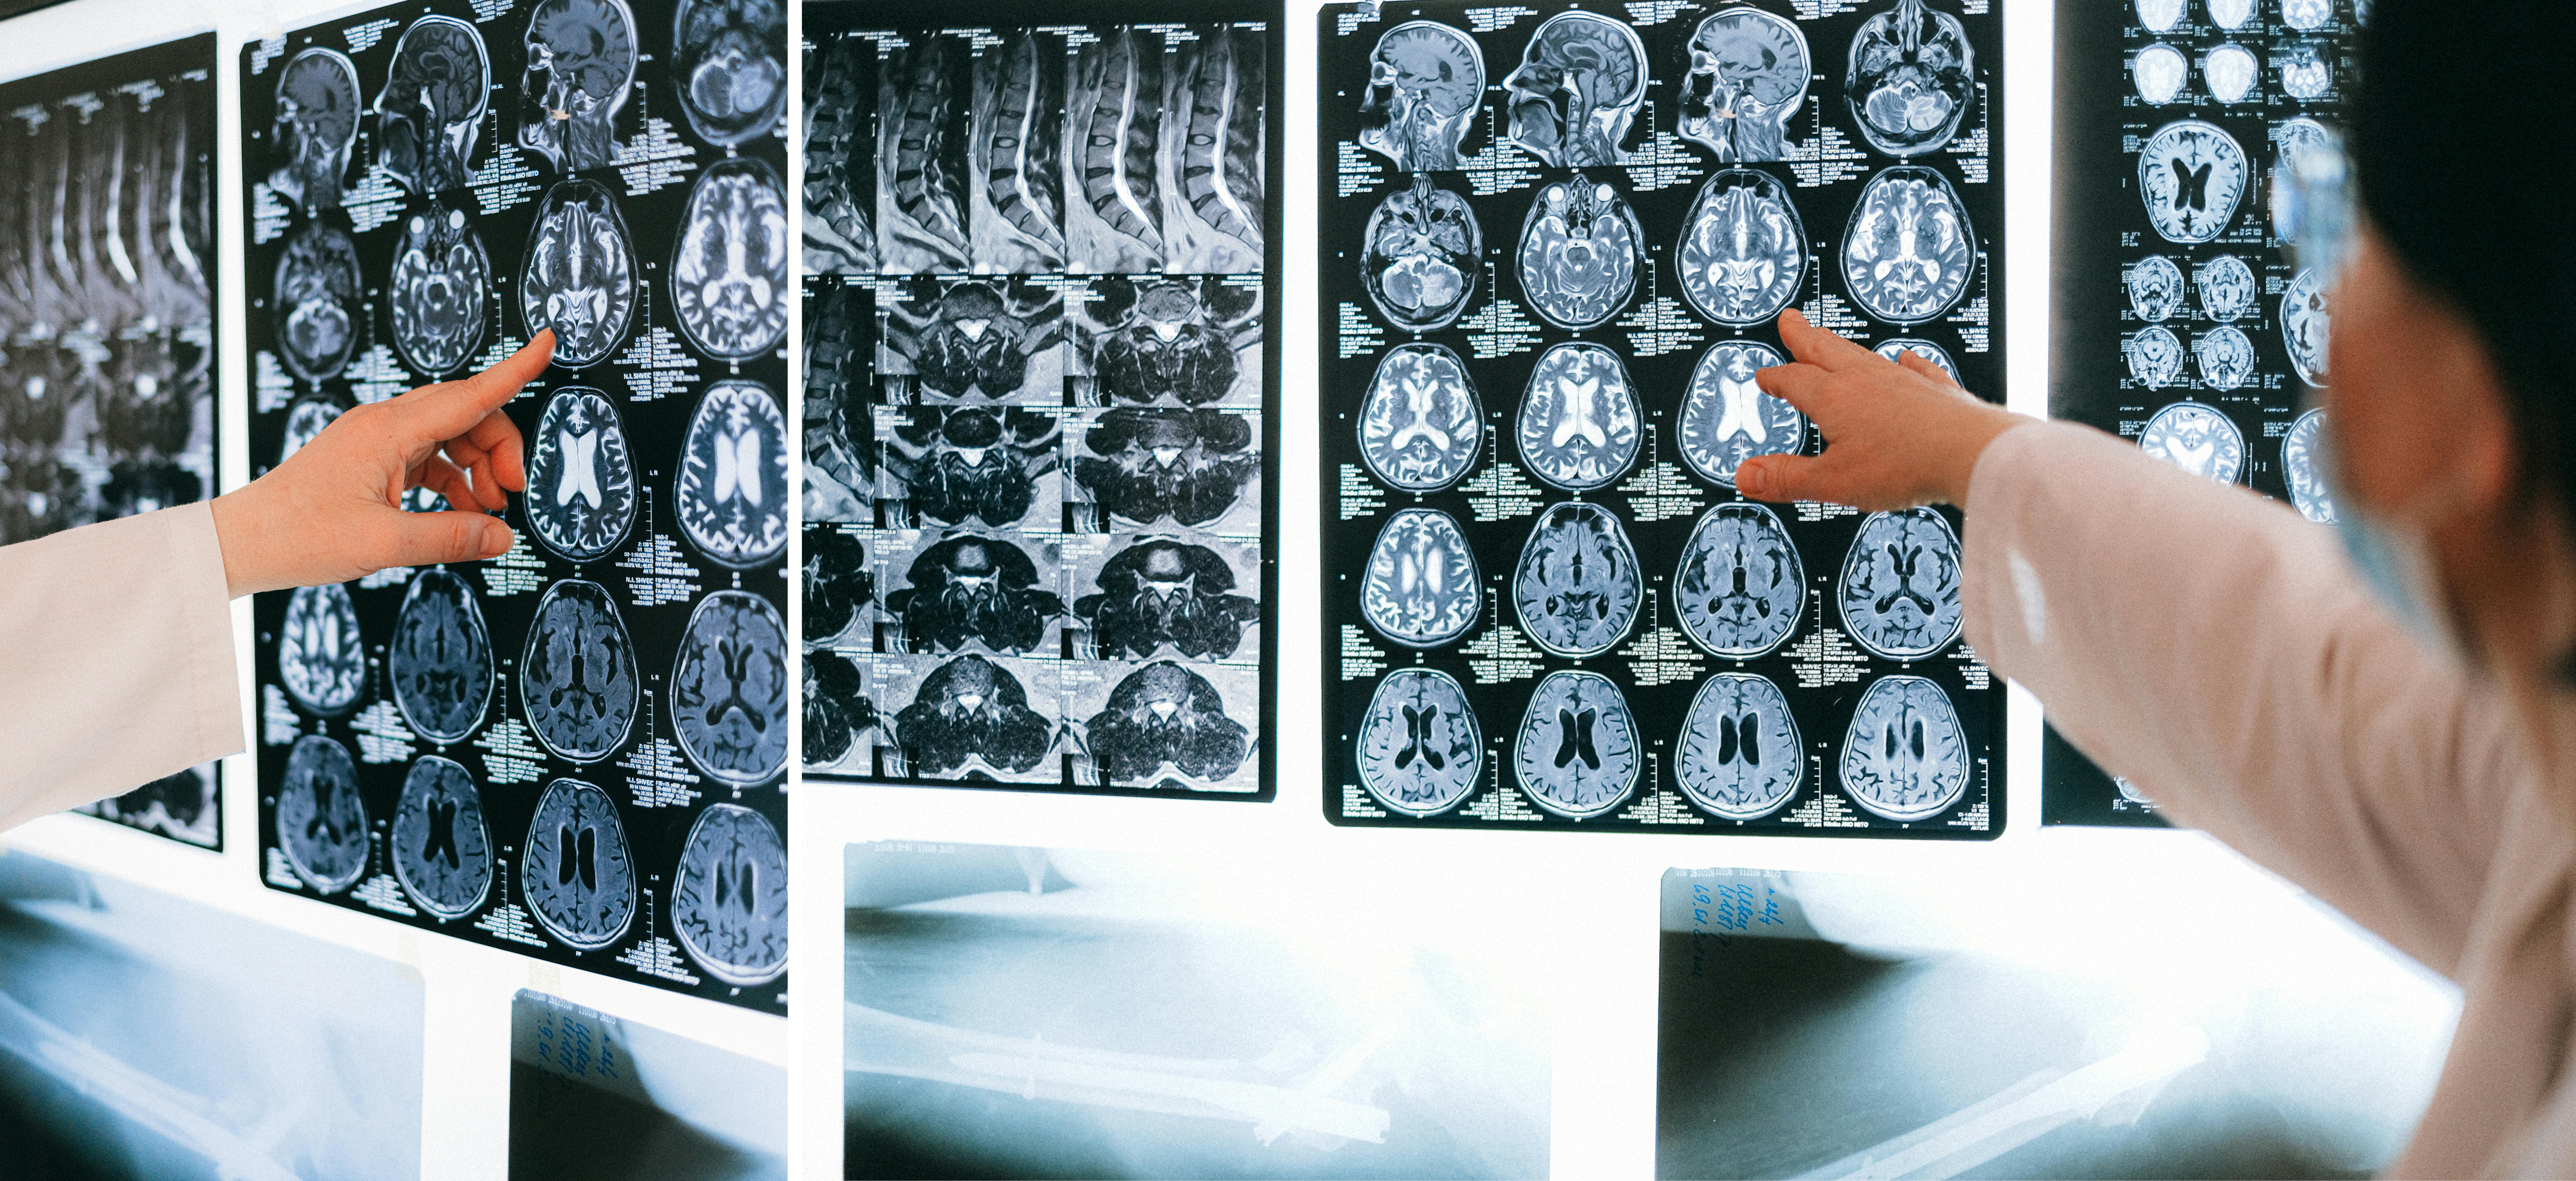
\includegraphics[width=\linewidth]{Chapter1/Images/pexels-shvetsa-MedicalFilms.png}
    \caption[Images of \gls{ct} and \gls{mri} films being utilized in a medical setting.]
    {
        Images of \gls{ct} and \gls{mri} films being utilized in a medical setting. 
        Anna Shvets took the photos shown here, which were licensed under a Creative Commons \DIFdelbeginFL \DIFdelFL{Attribuation }\DIFdelendFL \DIFaddbeginFL \DIFaddFL{Attribution }\DIFaddendFL licence~\footnotemark
    }
    \label{fig:MedicalFilms}
\end{figure}

Medical visualizations are commonly designed with 2D data in mind, as these tend to be viewed on desktop displays or tablets, or by more traditional display methods like placing films on light boxes and lit boards.  
2D visualizations require training in order to understand them, however experienced users can make more confident decisions with them due to understanding the structure of the human body~\cite{Jurgaitis2008}. 
Traditionally, \gls{mri} and \gls{ct} scans are printed onto transparent films and placed on adjustable light displays as shown in \autoref{fig:MedicalFilms}.~\footnotetext{\url{https://www.pexels.com/cs-cz/foto/ruka-doktor-ukazovani-lekar-4226264/}}
These adjustable light displays allow different scan slices to be visible in the film. 
These films are not easy to interpret for people without proper training.


Display technology employed to view tomographic data in radiology and related fields can significantly impact data interpretation.
Most medical visualizations displayed on a desktop typically represent 2D slices through the body.
Desktop and tablet interfaces will normally display this data in three different axesΓÇöone each for depth, width, or breadthΓÇöwith an additional display presenting a 3D model for spatial awareness~\cite{Mandalika2018, Mast2019}.
This limitation may lead to solutions that only consider the primary axis.
This would allow surgeons to perform surgeries with more flexibility than they would currently be comfortable with~\cite{Dicken2005}.
3D visualizations in some situations have been observed to be easier to understand, like identifying the distance between the operating area and high-risk areas or different methods to access the infected area~\cite{Dicken2005, Rieder2009, Cheung2021}.
This indicates that surgical planning could be further optimized and enhanced if 3D visualizations were displayed in a technically correct manner which is also contextually appropriate rendering and presentation. on their given displays and in the representative display environment. 

\begin{figure}
    \centering
    \includegraphics[width=\columnwidth]{Chapter1/Images/CTandMRIScan.png}
    \caption[Two similar slices of different human heads.]
    {
        Two similar slices of different human heads: on the left, one a Magnetic Resonance Imaging (MRI) scan\footnotemark[1]; and on the right a Computed Tomography (CT) scan\footnotemark[2]. Both these images are licensed under a Creative Commons Attribution license.
    }
    \label{fig:CTAndMRI}
\end{figure}







On desktop displays, 2D visualizations can present shapes more clearly than 3D visualizations~\cite{Abbey2021, Zhou2022}. 
However, stereoscopic 3D displays (\gls{ar} and \gls{vr}) have been shown to represent 3D medical data as effectively as, or even better than, 2D visualizations~\cite{McIntire2012}.
Surgeons can navigate data from any angle, leading to a more intuitive presentation and greater precision~\cite{Ahlberg2007, Zhang2016a, Akpan2019}. 
These findings suggest that stereoscopic immersive \glspl{hmd} allow users to perceive 3D data naturally and intuitively~\cite{Vetter2002, Merino2018, Cecotti2021}. 
Most research on medical \gls{ar} has focused on 2D visualizations~\cite{Asadi2024}, likely due to the challenges that still need to be addressed in using immersive \gls{ar} devices for medical applications.


\footnotetext[1]{\url{https://www.flickr.com/photos/reighleblanc/3854685038}}
\footnotetext[2]{\url{https://pixabay.com/photos/head-magnetic-resonance-imaging-mrt-254863/}}
The use cases for \gls{ar} in medicine are inspiring, but there is a range of limitations that need to be addressed before \gls{ar} becomes common practice~\cite{Jha2021, Beams2022}. 
Firstly, medical practitioners may not risk losing sight of the real world~\cite{Beams2022}. 
This can happen by placing any camera-based or occlusive display over the user's eyes. 
This makes a \gls{vst} \gls{ar} \glspl{hmd} solution difficult because these systems have the potential to partially blind the user if they are unplugged or disconnected~\cite{Beams2022}.
Systems that are designed for robotic surgery that utilize a video-based surgery tend to use a robotic arm with inbuilt measures for removing any apparatus from the patient where a well-trained expert can aid the situation~\cite{Rosen2011}, preventing any issues that can occur from minor distortions of the input images. 
\gls{ar} \glspl{hmd} currently show a distorted view of reality, which can negatively influence depth perception and mislead users when performing precise interactions depending on the real world environment~\cite{Bichlmeier2007, Sielhorst2006}.
\gls{ost} \gls{ar} avoids the limitation of superimposing the real world with the virtual world. However, because this technology simply overlays information over the screen and covers the user's eyes, it still faces limitations in how the virtual world is perceived in comparison to the real world.

\gls{ost} \gls{ar} devices misrepresent users' depth perception compared to real-world vision, even under ideal conditions. 
These devices are not designed to fully align the virtual world with the user's perception, offering a view of the real world that is 'good enough' for most applications. 
Some \gls{ar} displays, such as \gls{ost} \gls{ar}, and sensors, like infrared cameras, struggle under bright lighting conditions. 
This causes inconsistent sensor readings and may reduce display visibility due to the \gls{ost} \gls{ar}'s shaded lens used to reflect light as a display~\cite{Geng2013, Xiong2021}. 
This shaded lens struggles to render transparent objects and can mandate a limited color gamut~\cite{Geng2013, Xiong2021}.
This lack of visibility and distortions caused by the display diminish users' spatial awareness of the \gls{ar} graphics~\cite{Jamiy2019, Rosales2019, Al-Kalbani2019, Armbruster2008}. 
These issues are less pronounced with mobile \gls{ar} and \gls{vst} \gls{ar} displays~\cite{Krevelen2010, Martin-Gomez2021}. 

\gls{ost} \gls{ar} devices all misrepresent their users' real depth perception compared to their real-world vision, even under ideal circumstances.
\gls{ar} devices are not designed to fully align the virtual world with the user's vision; they provide a good enough world viewpoint into the real world.
Some \gls{ar} displays (like \gls{ost} \gls{ar} displays) and sensors (such as infrared cameras) do not work under bright lighting conditions as they dim the colors shown in the display and introduce inconsistent sensor readings. 
Users' spatial awareness is also lessened when viewing graphics using \gls{ar}~\cite{Jamiy2019, Rosales2019, Al-Kalbani2019, Armbruster2008}. 
\gls{ost} \gls{ar} require a shaded lens to properly reflect light back at the users~\cite{Geng2013, Xiong2021}. 
These issues do not exist as much with mobile AR~\cite{Krevelen2010}. 
\gls{ost} \gls{ar} displays also have difficulties when rendering transparency due to their limited color gamut and how it is used to inform brightness~\cite{Geng2013, Xiong2021}.

This dissertation explores methods for visualizing spatial data to ensure AR-rendered graphics seamlessly integrate with physical-world objects, such as the human body. 
A key challenge for any AR system is accurately presenting objects located within or behind other objects~\cite{Bajura1992, Avery2009, Kalkofen2013, Parsons2021}.
To understand the data's location, humans typically need specific cues to perceive an object inside another, such as occlusion or a real-world metaphor like a hole. Without these cues, the data often appears to hover in front of the occluding object, giving the impression that it is positioned incorrectly.

This research utilizes volume data as a medium, a 3D representation of space representing a set of samples from a given position relating to a given value in this area of the given voxel~\cite{Kaufman1999}.
volumes data allows this dissertation to move beyond traditional research by creating visualizations that utilize \gls{dvr}, allowing dynamic adjustments based on spatial and occlusion cues. 
This will enhance depth perception and improve integration with the physical environment. 
\gls{dvr} still allows for the same functionality as other graphical formats but provides new stereoscopic challenges that need to be overcome.
This dissertation also employs an off-the-shelf optical see-through (OST) AR device, the HoloLens 2~\footnote{\url{https://www.microsoft.com/en-au/hololens}}, which uses a lightly shaded lens and a waveform display to render images to ensure repeatability and consistency in testing these visualization techniques.





\section{Motivations} \label{sec:IntroMotivations}


Augmenting the real world using wearable devices (esp. \glspl{hmd}) is a promising field that has received much attention recently. Augmenting can take many forms, but seeing through or inside objects is particularly interesting in several domains.
It is common for immersive medical visualizations to present volume data as a 3D model so that it can be viewed from any direction. 
\glspl{hmd} allow for a natural way to view 3D data as users change their perspective by moving around the volume~\cite{Kasprzak2019, Pratt2018}.
\glspl{hmd} can be integrated with current systems to extend current working practices like cardiography~\cite{Kasprzak2019} and pathology~\cite{Hanna2018}. 

Hanna et al.~\cite{Hanna2018} looked into the potential of \gls{mr} within \gls{pathological} use cases, for example, enabling remote communication for autopsies for guidance and instruction using a 3D overlay and sharing scanned copies of specimens. 
\Glspl{pathologist}, like many medical professionals, are required to be able to keep a sterile environment. 
\gls{ar} \glspl{hmd}, like the HoloLens, utilize gesture commands that can keep an environment sterile and avoid with a keyboard and mouse which may contaminate the space.
This hands-free interaction is particularly beneficial in medical situations where sterility is paramount.



\begin{figure}
    \centering
    \includegraphics[width=0.8\textwidth]{Chapter1/Images/HannaEtAlAutopsyHoloLensExample.PNG}
    \caption[A image of Hanna et al.'s~\cite{Hanna2018} sterile system for \glspl{pathologist}]{A image of Hanna et al.'s~\cite{Hanna2018} sterile system for \glspl{pathologist}. Used with permission from the College of American Pathologists}
    \label{fig:HannaEtAlAutopsyHoloLensExample}
\end{figure}

A wide range of medical visualizations fall outside the scope of volumetric data
but benefit from 3D medical visualizations by using \gls{gui} in conjunction with \gls{ar}. Endoscopies use a long flexible tube with a camera and light at one end to examine the inside of the body. Immersive approaches have created visualizations that hover above the body to provide medical practitioners with an indication of where inside of the body they are looking~\cite{Garcia-Vazquez2020}. Other visualizations have focused on guiding the practitioner with a Graphical User Interface (GUI) so they can either instruct people on what to expect in a given situation, like explaining to a nurse what tools she might be expected to use next~\cite{Unger2019}, or they could be used to try to communicate the angle and direction an incision should be performed using a 2D GUI projected on the area around the patient~\cite{Mewes2018}.
These applications could benefit from better in situ visualizations at a single point, providing a more natural interface and a more intuitive sense of data. 

Research has explored overlaying a visualization for instructing a practitioner on using a syringe~\cite{Agten2018, Li2019a}.
Overlaying a \gls{mri} or \gls{ct} visualization has also been attempted on several occasions where it was found to to ensure that the medical practitioner can focus on what they are doing while observing the patient spontaneously and also the practitioner with annotations and instructions~\cite{Pratt2018, Si2018, Pratt2018, Blum2012}.
Visualizations can also educate the internal anatomy to less experienced practitioners or novices~\cite{Bajura1992}.

\subsection{Siemens Internship: Holographic Overlay System}

\begin{figure}
    \centering
    \includegraphics[width=0.8\textwidth]{Chapter1/Images/HolographicOverlaySystem.png}
    \caption{The Holographic Overlay system in use with a CT scanner.
}
    \label{fig:HolographicOverlaySystem}
\end{figure}

Enabling medical practitioners to more intuitively understand their patients and helping to ease the education of medical data are intuitive benefits to companies specializing in creating machines to produce this data. 
The benefits of data overlay formed the basis of an early internship I undertook at Siemens in Forchheim, Germany, where I explored the challenges still present in using scan data overlaid on patients' bodies.
At the commencement of this Ph.D. I was supported to travel to Siemens Forchheim, Bavaria, Germany, as an intern in the School of Health Sciences Digital Imaging \gls{ct} Research and Development Circulating Tumor Cells \gls{ai} department
I was asked to create a system capable of overlaying the volumetric data from a CT scanner and calibrating it to the bed of a \gls{ct} scanner so it could be overlaid on the patient.
This allows radiologists to view the patient data as it is overlaid onto the patient and communicate with the current status of the \gls{ct} machine to track the patient.


I was tasked with bringing the Booij et al.~\cite{Booij2019} research, which focused on a 2D interface that used a Kinect to collect a patient's anatomical data to aid radiologists in placing electrodes in the correct position on the patient's body utilizing a 3D reconstruction of the patient's body. 
The correct placement of electrodes on a patientΓÇÖs body can be a difficult procedure to learn as it requires knowledge of where certain organs exist.
It is possible to determine where to place an electrode by evaluating the shape of the patient's body. 
An issue with the Booij et al.~\cite{Booij2019} system is that a 2D representation of a human is not always an accurate guide for varying body types since organs, muscles, and other body parts may be misplaced causing significantly different results~\cite{Kania2014,Hadjiantoni2021}.
By using a 3D \gls{hmd}, \gls{ar} display (HoloLens1), a 3D overlay could be made to instruct any operator of the \gls{ct} machine on how to use the system. 

After the CT scan had been completed, the system would replace the electrode guidance functionality with a visualization slice on a Sagittal Plane of the radiological data. 
This was replaced in the 3D system with an iso-surface or a \gls{dvr} visualization that was to be superimposed over the patient's body to better guide and inform the operator of the quality of the \gls{ct} scan.
This was aimed at lowering the required learning for \gls{ct} operators. 

The gantry bed would need to be tracked, and its position known relative to the patient and the \gls{gantry} to provide the radiologist with instructions on where to place electrodes~\cite{Booij2019}. 
This allowed the volume to be visualized wherever the patient was, and it also provided flexibility for the operator to apply the electrodes. 
The final results of this system can be seen in \autoref{fig:HolographicOverlaySystem}.
The technical details of this system are described in more detail in \autoref{App:HolographicOverlaySystemDetails}.

Porting \gls{dvr} to a \gls{hmd} \gls{ar} display revealed more challenges than anticipated, primarily due to the high processing cost and the resulting visualization appearing slightly distorted in comparison to the surrounding environment.
This distortion was likely caused by the limited depth cues provided by \gls{ost} \gls{ar} displays, which made it difficult for users to determine the correct spatial position of virtual objects when physical objects were already present in the same location~\cite{Petri2018}.

One issue that was noted with the system was that the visualization was not dynamic and was only able to show a subset of a single range of the data before requiring to reload the information.
What was \DIFdelbegin \DIFdel{disired }\DIFdelend \DIFaddbegin \DIFadd{desired }\DIFaddend was the ability to view all of the data in a dynamic manner such as \gls{dvr}.  
For medical imaging, this capability is critical because important diagnostic features may not be confined to a single slice or range but distributed throughout the entire scan volume.
Being able to see the whole volume at once allows users to explore the data more intuitively and avoid missing relevant anatomical details or pathologies.
Particularly those with less specialized radiology training.

A prototype visualization of this can be seen in \autoref{fig:SiemensVolumeRendering} which presents a cube rendered with \gls{dvr}, showing the same inflated abdomen dataset as in \autoref{fig:HolographicOverlaySystem}, developed at Siemens Healthineers.
This visualization has several issues when viewed through an \gls{ar} display (Microsoft HoloLens), the visualization initially appeared to be in the correct spatial position. However, the stereoscopic properties of the \gls{hmd} made it evident that the visualization was rendered as a cube rather than a volumetric structure.
As a result, this method was ultimately excluded from the final version of the product.

\begin{figure}
    \centering
    \includegraphics[width=0.8\textwidth]{Chapter1/Images/VolumeRendering.png}
    \caption[This is a image of a cube rendered to show the same data shown in \autoref{fig:HolographicOverlaySystem} but using \gls{dvr}.]
    {
        This is a image of a cube rendered to show the same data of an inflated abdomen shown in \autoref{fig:HolographicOverlaySystem} but using \gls{dvr} which was developed at Siemens Healthineers.
    }
    \label{fig:SiemensVolumeRendering}
\end{figure}

\autoref{fig:HolographicOverlaySystem} depicts a challenge with the Holographic overlay system.
All of the visualizations that were supposed to be inside of the patient appeared smaller and outside of them. 
With enough time, users learned to orient themselves around this issue. 
This presentation of the data via \gls{ar} \gls{hmd} in this format seemed to cause more confusion about anatomy than simply displaying it on an external monitor or sitting above the patient.


Overall, my Internship at Siemens highlighted that the current AR technologies were limited, including:
\begin{enumerate}
    \item When placing virtual objects behind or within real-world objects, there is a visual mismatch that occurs, causing the virtual object to appear misaligned. This issue is due to the difficulty in judging depth due to the lack of depth cues~\cite{Petri2018}.
    \item Sub-centimetre precision poses a general challenge for visualization and perception using \gls{mr} devices. The effect of \gls{ost} \gls{ar} visualizations on the user's depth perception requires further investigation.
    \item There currently exists no standard method to present frequently changing volumetric data inside an object.
\item Medical information is often represented as volumetric data with continuously varying properties, rather than as discrete surface objects.
    Allowing for more direct contextual customization of the visualizations in real time paired with the ability to see the entire volume at once not just the given surfaces of a set range.
    Conventional polygonal rendering methods struggle to represent this type of data in a complete and integrated way.
\end{enumerate}










\section{Research Goal} \label{sec:IntroReserachGoal}


This research seeks to investigate the use of \gls{dvr} within physical objects when using \gls{ost} \gls{ar} \gls{hmd}s. 
The holographic overlay system displayed this data out of place.
\autoref{fig:DiagramX-rayVision} shows that the visualization is positioned correctly compared to the camera. However, because it is superimposed, it appears much larger and closer to the viewer. 
This was identified as a challenge to be addressed before systems become practical.


X-ray vision has been shown to repair this issue using virtual holes~\cite{Bajura1992}. 
However, this solution is not perfect. 
X-ray vision focused on medical situations, and many of the solutions were designed to accommodate \gls{vst} display technology rather than \gls{ost} \glspl{hmd}, which is not practical in a medical situation~\cite{Wang2017a}.
The solutions appeared to restrict the users' view of the data, making tasks like determining the \gls {ct} scan quality more challenging than needed.
The visualizations also utilized static geometry to generate the X-ray visualization while preventing the required level of flexibility.





\begin{figure}
    \centering
    \includegraphics[width=1\linewidth]{Chapter1/Images/DiagramX-rayVisionMoreDetail.png}
    \caption{
        An example of where it is difficult to interpret depth due to the absence of depth cues. The circular object is a virtual object displayed against the wall in the next room. 
        \textbf{Left}) shows the room with no X-ray vision; \textbf{center}) shows the same room with X-ray vision enabled. However, the lack of depth cues makes it impossible to determine where the circular object in the next room is located. 
        \textbf{Right}) shows the same rooms as on the left, displayed using an isometric perspective to illustrate where the items are actually located.
    }
    \label{fig:DiagramX-rayVision}
\end{figure}

The high-stress occupations found in medicine demand a level of predictability from the tools that they use. 
The influence on X-ray vision's ability to hinder perception has previously been tested~\cite{Santos2015}, but how it obscures spatial understanding is still unknown. 
There are also many unknowns about the ecological effects of X-ray vision, as most research in this area has mainly focused on perceptual tasks. 



\gls{dvr} itself has not been utilized on \gls{ost} \gls{ar} devices, despite having many applications in the medical domain alone. 
This, in turn, indicates there are a plethora of unknown consequences that may arise from its utility. 
While creating X-ray visualizations that are designed to suit the \gls{ost} \gls{ar} display, it is important to note that these visualizations need to both suit the tasks they are required for and simultaneously function regardless of the use case. 
Ensuring these visualizations should suit the purposes where viewing \gls{dvr} information within the object itself is relevant, regardless if they are referring to manufacturing~\cite{Kanodia2005}, biological~\cite{Guo2012} or surgical tasks~\cite{Bajura1992}. 
These visualizations should be designed to allow users to view surfaces of any shape. 
X-ray visualizations should improve depth perception while allowing users to gain insight into the volume quickly.


















The following factors motivate this research to focus on investigating:
\begin{itemize}
    \item How DVR techniques can be developed for OST AR, particularly for X-ray vision;
    \item If visual cues may aid in understanding spatial arrangement and relative depth perception;
    \item Observing the effects of visual cues and the accuracy that can be achieved on an \gls{ost} \gls{ar} \gls{hmd} display.
\end{itemize}

















\section{Research Questions}
To address the research goals listed in \autoref{sec:IntroReserachGoal} focusing on creating \gls{X-ray Vision} methods for \gls{dvr}. 
This thesis will explore the following questions:

\begin{enumerate}[label=R.\arabic*]
\item How do X-ray visualization effects influence how accurately users can perceive the spatial alignment of a virtual object embedded within a real-world object? (Chapter 3);
\item Can \glspl{virt} aid a personΓÇÖs comprehension of a volume when determining individual objects using direct volume rendering?  (Chapter 6);
    \item What is the minimum difference in depth that participants can reliably distinguish between volumetric objects, independent of any given \gls{virt}? (Chapter 7);
\end{enumerate}

\section{Contributions}
This thesis contributes the following:
\begin{enumerate}[label=C.\arabic*]
    \item A systematic literature review of \gls{X-ray Vision} describing the work to date. Presents an overview of the studies performed and an analysis of the use cases. (presented in Chapter 2, published in P.3);
    \item An algorithm that allows VST AR x-ray visualizations to be displayed on an OST AR device. (described in Chapter 3, published in P.4);
    \item Adapting X-ray techniques from \gls{vst} \gls{ar} to \gls{ost} \gls{ar}. (Presented in Chapter 4, published in P.6);
    \item A study comparing \gls{X-ray Vision} effects that had only previously been used on \gls{vst} \gls{ar} to be viewed on OST AR device. Showing that geometry-based \gls{X-ray Vision} techniques were better suited to OST AR devices (presented in Chapter 3, published in P.4);
    \item implementation of Volumetric \gls{X-ray Vision} utilizing Volumetric Illustrative Rendering \DIFdelbegin \DIFdel{Technqiues }\DIFdelend \DIFaddbegin \DIFadd{Techniques }\DIFaddend (VIRTs). (described in Chapter 4, published in P.6);
    \item The Random Volume Generation System. A tool to randomly generate volumes that allow for controlled user studies in \gls{X-ray Vision}. (presented in Chapter 5, published in P.5); 
    \item A perception-based counting study to determine how well users could see the three VIRTs created. Findings show that different VIRTs could negatively and positively impact a user's ability to perceive accurately and determine what elements were in a volume. (presented in Chapter 6);
    \item A study to determine the different perceivable depth thresholds that the Hatching Stippling and Halo VIRTs can have between each other and a baseline condition by utilizing a 2FCA psychophysical study design. (presented in chapter 7);
\end{enumerate}

\section{List Of Publications} \label{section:Publications}
\begin{enumerate}[label=P.\arabic*]
    \item \textbf{Clarke, T. J.} (2021). Depth Perception using X-Ray Visualizations. 2021 IEEE International Symposium on Mixed and Augmented Reality Adjunct (ISMAR-Adjunct), 483ΓÇô486. https://doi.org/10.1109/ISMAR-Adjunct54149.2021.00114
    \newline
    Contributed To: 
    \begin{itemize}
        \item Chapter 1;
    \end{itemize}

    \item Smith, R. T., \textbf{Clarke, T. J.}, Mayer, W., Cunningham, A., Matthews, B., \& Zucco, J. E. (2020). Mixed Reality Interaction and Presentation Techniques for Medical Visualisations. In P. M. Rea (Ed.), Biomedical Visualisation: Volume 8 (pp. 123ΓÇô139). Springer International Publishing. https://doi.org/10.1007/$978-3-030-47483-6_7$
    \\
    Contributed To: 
    \begin{itemize}
        \item Chapter 1;
        \item Chapter 2;
    \end{itemize}

    \item \textbf{Clarke, T. J.}, Gwilt, I., Zucco, J., Mayer, W., and Smith, R T. (2024) Superpowers in the Metaverse: Augmented Reality Enabled X-Ray Vision in Immersive Environments. In Geroimenko V., Augmented and Virtual Reality in the Metaverse.
    \newline
    Contributed To: 
    \begin{itemize}
        \item Chapter 2;
    \end{itemize}

    \item \textbf{Clarke, T. J.}, Mayer, W., Zucco, J. E., Matthews, B. J., \& Smith, R. T. (2022). Adapting VST AR X-Ray Vision Techniques to OST AR. Proceedings - 2022 IEEE International Symposium on Mixed and Augmented Reality Adjunct, ISMAR-Adjunct 2022, 495ΓÇô500. https://doi.org/10.1109/ISMAR-Adjunct57072.2022.00104
    \newline
    Contributed To: 
    \begin{itemize}
        \item Chapter 3;
    \end{itemize}

    \item \textbf{T. J. Clarke}, W. Mayer, J. E. Zucco and R. T. Smith, "Generating Pseudo Random Volumes for Volumetric Research," 2023 IEEE International Symposium on Mixed and Augmented Reality Adjunct (ISMAR-Adjunct), Sydney, Australia, 2023, pp. 266-270, doi: 10.1109/ISMAR-Adjunct60411.2023.00061.
    \newline
    Contributed To: 
    \begin{itemize}
        \item Chapter 4;
    \end{itemize}

    \item \textbf{T. J. Clarke}, W. Mayer, J. E. Zucco, A. Drogemuller and R. T. Smith, "Volumetric X-ray Vision Using Illustrative Visual Effects," 2023 IEEE International Symposium on Mixed and Augmented Reality Adjunct (ISMAR-Adjunct), Sydney, Australia, 2023, pp. 769-771, doi: 10.1109/ISMAR-Adjunct60411.2023.00168.
    \newline
    Contributed To: 
    \begin{itemize}
        \item Chapter 5;
    \end{itemize}



\end{enumerate}

\section{Dissertation Structure}
Following this chapter is the literature review (Chapter 2), which will focus on all the related research done on \gls{mr} with a focus on medical applications, followed by a look into the research done on \gls{hci} regarding volumetric data and finished with a systematic literature review on \gls{X-ray Vision} covering all of the previous work done over the past 31 years in this field. 



The results from the literature review were used to inform the study in Chapter 3, which looks at a variety of popular \gls{X-ray Vision} effects that are designed to utilize a range of different \gls{ar} \gls{hmd}s. 
To achieve this, a system was developed that allows \gls{vst} \gls{ar} techniques to be used on \gls{ost} \gls{ar} devices. 
This system was then used to perform a spatial estimation task, enabling an in-depth evaluation of how these effects function across different augmented reality hardware configurations.

Chapter 4 investigates the technical work involved in volume rendering and details the complexities involved in creating \gls{dvr} techniques for X-ray vision, concluding in the creation of the Volumetric Illustrative Rendering Techniques (VIRTs). 
This was followed by a modular method to create random volumes and details, the Random Volume Generation system. The Random Volume Generation system allows controlled studies to be conducted with volumes to access the VIRTs (described in Chapter 5).
The combination of the Random Volume Generation system and the VIRTs is then utilized in Chapter 6 to run a perception-based user study designed to determine how well a user can count regions within a volume. 
The chapter (Chapter 7) then took the VIRTs and tested the degree of depth thresholds users could reliably distinguish depth by utilizing a 2FCA psychophysical study.
The final chapter draws together the results and findings of this dissertation (Chapter 8).

\clearpage{}
\glsresetall
    \clearpage{}\chapter{Background} \label{chap:Background}
This section begins by exploring the history of human vision research, tracing its development to our current understanding of human perception and its integration with \gls{mr} hardware.
We then look at the research behind how depth perception and perception can be considered with \gls{mr} \glspl{hmd}.
Followed by a systematic literature review of \gls{ar} enabled \gls{X-ray Vision}.
The discussion then shifts to volume rendering, emphasizing human-centered research using \gls{dvr}, and concludes with an analysis of illustrative effects and their applications within \gls{dvr}.



\section{Human Perception and Depth Perception}
\begin{figure}
    \centering
    \includegraphics[width=\textwidth]{Chapter2/Images/CuttingDepthGraph.png}
    \caption[This graph of depth cues and distance provides guidelines for depth perception in relation to the distance and key perception parameters.]{
    This graph of depth cues and distance provides guidelines for depth perception in relation to the distance and key perception parameters. Used with permission from Cutting and Vishton~\cite{Vishton1995}.
    }
    \label{fig:CuttingDepthGraph}
\end{figure}

Understanding the mechanisms of how perception works has been a goal for humans long before computing or \gls{mr} devices.
Perception has been studied since Democritus conceived that sight was formed from small indivisible particles (460-371 BC). 
Since then, we have learned the anatomical structures of eyes and that sight is processed in the mind rather than the eye (1011 - 1021).
During the 18th century, we started to gain a more modern view of how people see light (based on the reflection of light off of other objects), and we began to learn about how we observe beauty, aesthetics, and apparent deceptions. 
Newton's particle theory in \DIFdelbegin \DIFdel{Opticks }\DIFdelend \DIFaddbegin \DIFadd{Optics }\DIFaddend (1704) proposed that light is composed of small particles that travel in straight lines. These particles change direction and speed when they hit a reflective surface, dispersing into different colors. 
This started a revolutionary shift in our perception of light. Later findings disproved the belief in pure white light despite Goethe's defense of Aristotle's theory (1810).
This understanding of vision enabled technologies like motion images (developed in 1932), leading to the first motion picture projector (the Phantoscope) in 1895. 

In 1889, Gustav Fechner~\cite{alma9911190913502466} coined psycho-physical, and we developed a metric for quantitatively determining changes in people's perception.
Their study involved seeing at what point a user could no longer determine if more or fewer dots were in a pair of images. 
All pairs of images had ten more or fewer dots than the other one. 
This study showed that the more dots placed on a page, the harder it is for someone to determine the difference, creating the foundation of psychophysics analytics~\cite{alma9911190913502466}. 
From this point, qualitative experiments on perception began to run, and it became possible to understand precisely how human perception functioned.
Leading to our current understanding of topics like depth perception.

\subsection{Depth Perception Fundamentals}
Throughout the late 19\textsuperscript{th} century and the 20\textsuperscript{th} century, psychologists began to study depth perception and came up with many factors to describe it.
Most of these findings believed that depth perception was created by utilizing accommodation, convergence, motion perspective, binocular disparities, height of the visual field, aerial perspective, occlusion, and the relative size and density of objects~\cite{Vishton1995}.
In 1995, Cutting and Vishton took over a century's worth of research and concluded that the human ability to determine what parameters of depth perception are required to be effective.
Notably, not all depth cues are equal, and many are situational.
\autoref{fig:CuttingDepthGraph} shows a breakdown of how these depth cues can be contrasted based on how far away they are from each other. The obvious difference between the depth of two objects is shown using the virtual axis, while the horizontal axis shows the distance or the depth away from the viewer's vision they are effective. 

\begin{figure}[tb]
    \centering
    \includegraphics[width=\columnwidth]{Chapter2/Images/ThesisDepthPerceptionImage.png}
    \caption[Several images showing various cases of Monoscopic forms of depth perception]{Depth cues and placements:
    Several images showing various cases of monoscopic forms of depth perception
    a) Shows an example of Occlusion trees that are occluded behind the main tree;
    b) An example of relative size where the larger trees a tree is the further in the foreground it seems to be;
    c) The field's height where the trees are located higher up in the image will seem farther away from the user. 
    }
    \label{fig:ThesisDepthPerceptionImage}
\end{figure}

Different forms of depth perception can be described by their utility in other spaces (Illustrated in \autoref{fig:CuttingDepthGraph}). 
Personal space refers to anywhere within 2m of the viewer, giving the viewer the required depth perception to interact with objects.
The action space relates to any distance between 2 and 25m where depth perception functions by using the optical relationship between different objects.
The vista space works by utilizing the changes of color in the horizon~\cite{Vishton1995}. 

Occlusion is considered to have the most influence over any depth perception technique~\cite{Vishton1995} and is effective as long as both the occluder and the occluded are in sight. 
The user can tell what object is closer to them~\cite{Vishton1995}.
However, occlusion itself only reveals the order of these functions~\cite{Vishton1995}.
Occlusion power comes from it being such an obvious depth cue~\cite{Boring1942}, requiring only contrast, the opacity of objects, and the assumption that the object is not changing its shape without the viewer knowing about it. 

Relative size and density are based on the user's current knowledge of the world and only noticed a deduction in accuracy at distances past 5km away from the viewer~\cite{Bajura1992}. 
Relative size refers to someone's ability to determine depth based on how small it looks to them. 
Relative density refers to how densely these objects seem to be clustered together. 
\autoref{fig:RelativeDensityAndAerialPerspectiveExample} illustrates how together, these techniques discern the depth of field away from an object. 
If the users are familiar with an object, they can determine how far away it is. However, this is much more powerful when there is more than one object in the distance.
This depth cue, unlike occlusion, can be used to gain a more granular idea of depth. 

When looking off into the distance, objects may appear visibly lower the further away they are from the viewer.
This is the Height in the Visual Field shown in \autoref{fig:RelativeDensityAndAerialPerspectiveExample}.
This cue relies on the objects touching the ground, so things like airplanes are no good. 
This cue tends to work very well when an object is within several meters of a user (depending on its scale) and still works well up to about 1,000m away.

\begin{figure}[bt]
    \centering
    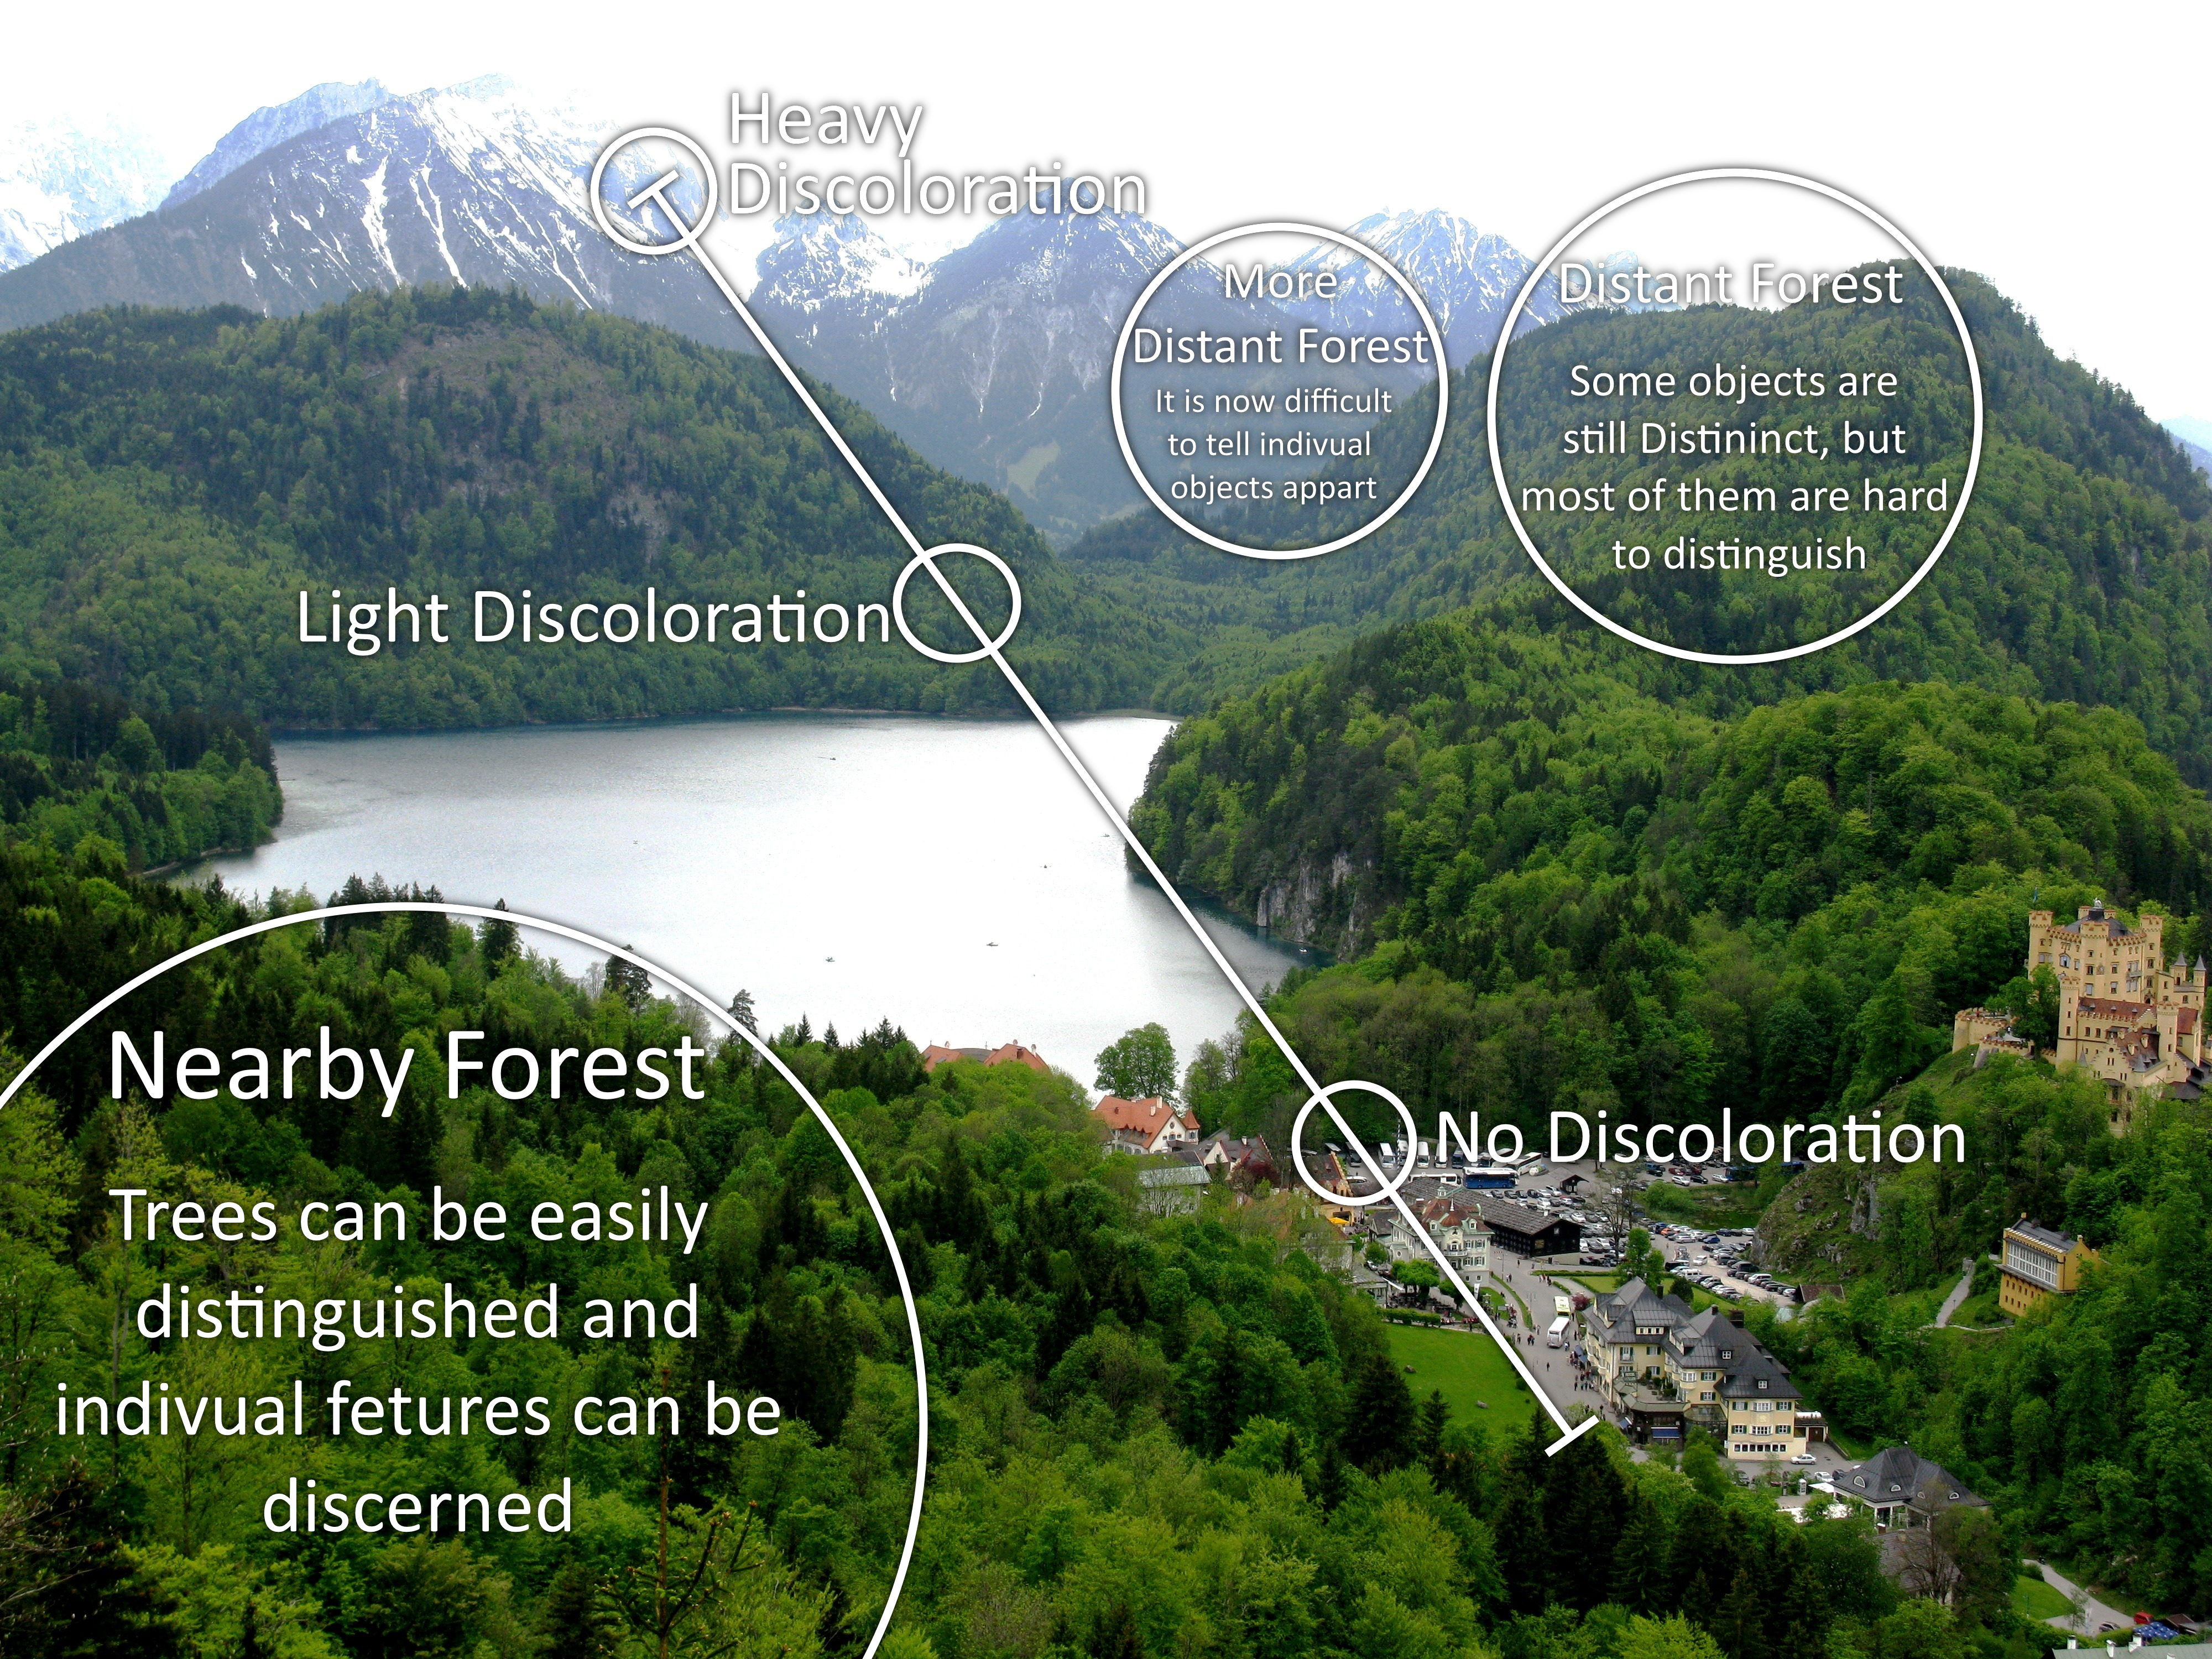
\includegraphics[width=\columnwidth]{Chapter2/Images/RelativeDensityAndAerialPerspectiveExample.png}
    \caption[Aerial Perspective, Relative Size, and Relative Density: An Image of a mountain view in Bavaria, Germany, with indicators to explain how monoscopic depth perception functions]{
        Aerial Perspective, Relative Size, and Relative Density: An Image of a mountain view in Bavaria, Germany. Several circles whose depths indicate how forests are viewed at various depths are shown. A line showing the gradual effects of the aerial perspective is also shown, indicating how it can be utilized to determine depth.
        The background image is licensed under a Creative Commons Attribution Universal 1.0 International license. 
        \footnotemark
    }
    \label{fig:RelativeDensityAndAerialPerspectiveExample}
\end{figure}

Aerial Perspective Refers to our ability to look through transparent objects. Generally, this refers to one's ability to look through the water in the air, making mountains look blue, and is also applicable underwater and when viewing gas-like elements~\cite{Vishton1995}.
Transparent objects can be pretty rare, so most of these elements will naturally be seen from a distance in \autoref{fig:RelativeDensityAndAerialPerspectiveExample}. 
This, however, may not be the need to be the case when using computer graphics~\cite{Vishton1995}.

\begin{figure}[tb]
    \centering
    \includegraphics[width=\columnwidth]{Chapter2/Images/Frenchetal.png}
    \caption[Depth Cues and Motion: Schematic illustration of motion components arising from observer translation and scene-relative object motion.]{Depth Cues and Motion: Schematic illustration of motion components arising from observer translation and scene-relative object motion~\cite{French2022}. (a) An observer fixates on a traffic light while moving to the right, as a car independently moves left. (bΓÇôd) Depiction of the car's image motion components related to self-motion and object motion. (d) accounts for image inversion by the eye's lens. (b) If the car is stationary, it shows a leftward image motion due to the observer's movement. (c) If the car moves left while the observer moves right, the car's image motion also includes an object motion component. (d) The net image motion of the car, vret, is to the right. This figure is licensed under a Creative Commons Attribution license and was produced by French and Deangelis~\cite{French2022}.}
    \label{fig:FrenchEtAl}
\end{figure}

\footnotetext{\url{https://pxhere.com/en/photo/965104}}
Motion parallax is considered the depth cue relating to how we perceive motion. 
This seems foundational to how we perceive depth~\cite{Lee1980}.
As seen in \autoref{fig:FrenchEtAl}, the motion perspective normally relies on the user viewer focusing on an object that is moving concerning them~\cite{French2022}. 
This could be looking at a ball they are about to catch or a house in the distance while a user passes it in a car or some other form of transport~\cite{French2022}.
Motion is an effective depth cue within 15 meters, but as \autoref{fig:CuttingDepthGraph} illustrates, the effectiveness lessens when the objects are further away from the viewer and declines when an object is within 2m of a viewer as they can't fully perceive the object~\cite{Shojiro1991}. 

People determine the depth perception of objects based on how their eyes are focused, which can also be a useful depth cue~\cite{Zannoli2016}.
\autoref{fig:AccomodationAndConvergenceInRealAndVirtualWorlds} illustrates how changing the accommodation and convergence allows us to focus on a given object.
Humans can change the disposition between their eyes~\cite{Berkeley1948}. 
Accommodation relates to the ability to change the shape for focus. 
Of the eye to see an object clearly and at different distances. 
Whereas convergence relates to the ability to turn the eyes to focus on nearby objects inwardly. 
These eye movement behaviours have a limited range, \autoref{fig:CuttingDepthGraph} shows at closer distances to us, this depth cue works the most effectively together, but it also shows as the eyes move farther apart, objects positioned further in front of or behind the focal point become increasingly blurred~\cite{Bajura1992}.

\begin{figure}[tb]
    \centering
    \includegraphics[width=\textwidth]{Chapter2/Images/AccomodationAndConvergenceInRealAndVirtualWorlds.png}
    \caption[A depiction of how convergence and accommodation work in the real world using Mixed Reality and OST AR.]{Convergence and Accommodation:
        A depiction of how convergence and accommodation work in the real world using Mixed Reality and OST AR. It consists of 4 diagrams showing how accommodation and convergence work together to better perception. The \DIFdelbeginFL \DIFdelFL{blured }\DIFdelendFL \DIFaddbeginFL \DIFaddFL{blurred }\DIFaddendFL ducks indicate a point where a duck would not be in focus to the viewer based on the position sitting in this position due to the effect of convergence and accommodation. The frames below show examples of the resulting perceived images of the objects in each diagram. Each of the four diagrams showcases a human eye (the circular object) viewing some ducks. The point where the eyes meet is their vergence or the point of convergence (depicted by the line). The cone represents the accommodation, which focuses on the physical distance the viewer is from the display. This image was inspired by work by Rosedaler. This is licensed under a Creative Commons Attribution licence~\footnotemark.
    }
    \label{fig:AccomodationAndConvergenceInRealAndVirtualWorlds}
\end{figure}

Since both eyes have a different view of the real world, the image each eyes perceive is inherently different.
This enables humans with several different abilities that are processed in the brain: 
\begin{itemize}
    \item \textbf{Stereopsis :} Refers to our human ability to assemble a 3D image from two 2D images from each eye. Giving us the ability to see the world in 3D. 
    \item \textbf{Diplopia :} Also called double vision. This is what occurs with binocular disparity, which can't be completely fixed by Stereopsis, leaving the viewer with two images that are not correctly aligned.
\end{itemize}
These cues give viewers a clear indication of how the world is around them and are referred to in combination as binocular disparities. 
Binocular disparities are more effective when viewed closer to the viewer as the further they are away from each eye, the similar position they are in each eye~\cite{Vishton1995}. 

Other cues can give a viewer a better sense of depth. 
For example, it is possible to directly tell the viewer how far things are by presenting them with a neat grid texture. Explaining to a user exactly how big a world is can obviously present a high level of depth perception. 
Objects with a high amount of contrast can also be clearer to see; however, this can be seen as improving the relief size and density.
Finally, humans may process depth perception in ways we have yet to understand fully; it is quite possible there is an aspect to living on earth, like gravity, that may even have an effect on our sense of depth perception~\cite{Vishton1995, Watson1992}.

\footnotetext{\url{https://commons.wikimedia.org/wiki/User:Rosedaler}}

\subsection{Research into the Depth Perception of Color}
This dissertation utilizes several colorful objects in its evaluations and creates two studies that directly utilize someone's ability to discern color from a specified area. 
This particular section highlights the papers of note that researched the impact of colors on depth perception.
By understanding this research, the changes in depth perception that various colors can provide were mitigated across this dissertation. 

Ping et al.~\cite{Ping2020a} highlight the impact that colors can have on depth perception.
When talking about medical visualization in general, it is very common to have several transparent layers in a single visualization.
Some research has found that people tend to \DIFdelbegin \DIFdel{precive }\DIFdelend \DIFaddbegin \DIFadd{perceive }\DIFaddend different colors as being closer or further away than others~\cite{Aoi2020, Ping2020a}.
This section of the thesis discusses the research that has been factored into considerations regarding how color influences depth perception. 

\begin{figure}[bt]
    \centering
    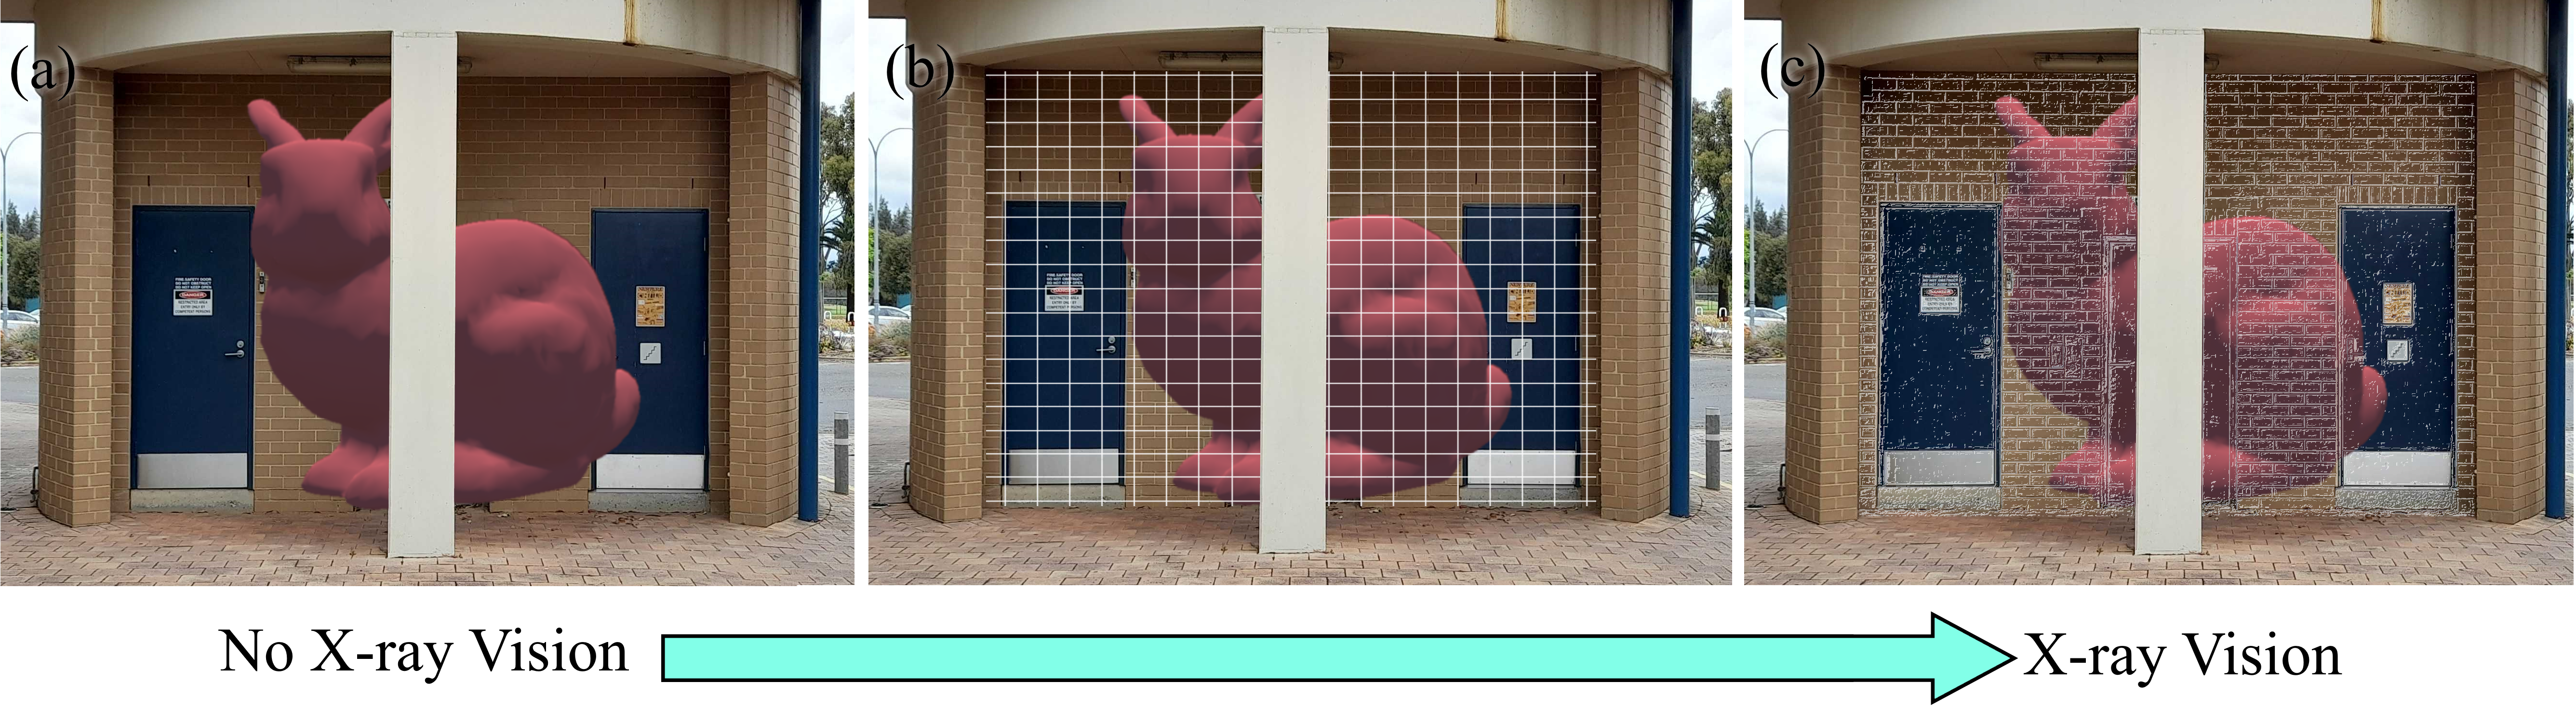
\includegraphics[width=\columnwidth]{Chapter2/Images/ARToXrayVision.png}
    \caption[Three images of the Stanford bunny sitting behind a wall, each using a different \gls{X-ray Vision} effect.]{Three images of the Stanford bunny sitting behind a wall, each using a different \gls{X-ray Vision} effect. To the left, a simple depth cue by placing the bunny behind a column. In the center, a virtual grid is placed over the physical wall to explain to the viewer that the bunny is behind the wall. On the right is highlighting the edge of the bricks with \gls{ar} using edge detection to indicate that the bunny is behind the wall.}
    \label{fig:ARToXrayVision}
\end{figure}

Aio and Li~\cite{Aoi2020} wanted to test how the luminance and Contrast affected the depth perception of transparent plans when viewed on a computer monitor.
The goal was to determine what methods could be utilized to make it more obvious which object was behind the other. 
They had two conditions to achieve this. They utilized luminance contact, testing the difference between changing the gradient between light and dark to dark to light.
They utilized four planes of different sizes to distinguish depth perception. 
This study was conducted using an autoscopic display, which allowed for the presence and absence of motion parallax and no binocular parallax, giving the participants extra depth cues.  
Throughout this study, Aoi and Li~\cite{Aoi2020} noticed participants underestimated depth perception but it could be improved by using either (or both) binocular parallax and \DIFdelbegin \DIFdel{motiion }\DIFdelend \DIFaddbegin \DIFadd{motion }\DIFaddend parallax. 
They also noted that occluding darker or lighter colors did not make much difference.
Aio and Li~\cite{Aoi2020} next utilized the information from their prior study to test this data on medical data and less difference between the choices of different colors. 

\section{Illustrative Rendering Techniques}
Cutting and Vishton~\cite{Vishton1995} claim there are several real-world elements to create depth perception, which then need to be adapted for virtual displays~\cite{Cutting1997}.
However, artists have been able to establish depth perception even when illustrating non-realistic environments by using "Just Enough Reality"~\cite{Siegel2000} to determine depth accurately.

The latter part of this thesis looks at using \glspl{virt} as a method of \gls{X-ray Vision}. 
Building on these perceptual foundations, the challenge in computer graphicsΓÇöand particularly in advanced visualization domains such as X-ray or mixed reality displaysΓÇöis not just to replicate the cues found in natural vision, but to enhance and adapt them for clarity and insight. 
While perceptual mechanisms like stereopsis and texture gradients provide a basis for spatial understanding, there are scenarios where simply mimicking the real world is insufficient. 
Here, artistic illustrative effects become invaluable: by deliberately emphasizing, abstracting, or revealing underlying structures, these techniques enable viewers to "see" information that might otherwise remain obscured. 
In this way, the migration from perception-driven rendering toward illustrative approaches is not only a technical evolution, but also a creative one, leveraging artistic conventions to extend the capabilities of visual communication in graphics.


This section is going to look at how these effects have previously been used, what their impact has been on computer science, and what their utility has been when using \gls{mr} devices.
While this thesis only looks into a subsection of illustrative techniques, limiting itself to either Hatching, Stippling, or Halos, the actual definition of this is broader~\cite{Lawonn2018}.
Illustrative techniques can also include the scope of non-photorealistic rendering, like using \DIFdelbegin \DIFdel{cel-shading }\DIFdelend \DIFaddbegin \DIFadd{cell-shading }\DIFaddend and the deformation of video footage to look like it was produced by a pencil or paintbrush~\cite{Lawonn2018}. 
This section will also examine some user studies that have investigated this effectiveness~\cite{Lawonn2018}. 

The largest examples of illustrative effects being used can be seen in scientific textbooks like Gray's anatomy~\cite{gray1877anatomy}.
This textbook utilized hatching's ability to communicate texture and depth using a black-and-white image.
These images were collected over years of diagramming the human body by directing unclaimed bodies from workhouses and mortuaries. Due to their clarity and accuracy, they are still widely used today. 

Early work in the field by Interrante et al.~\cite{Interrante1995, Interrante1997, Interrante1997a} looked at how illustrative effects can aid the perception of transparent objects.
Transparent objects make it difficult to understand the exact surface of the shape that a transparent object is formed as. 
This was done by pre-computing textures that used transparent and opaque regions.
The first work was done by creating several different textures, including multiple methods that depict valleys and ridges, grids, and curvature information~\cite{Interrante1995}. 

To improve the on \DIFdelbegin \DIFdel{thier piror }\DIFdelend \DIFaddbegin \DIFadd{their prior }\DIFaddend work~\cite{Interrante1995}, Interrante~\cite{Interrante1997a} created a visualization that utilized valleys, ridges, and curvature to explain the objects' flow. 
This texture was calculated by drawing lines around the parts of the mesh with the highest curvature and having them move toward the ridges and valleys of the shapes. 
This dissertation extends this \DIFdelbegin \DIFdel{resarch }\DIFdelend \DIFaddbegin \DIFadd{research }\DIFaddend by creating a texture that could be viewed from all sides, requiring less computation when the object is viewed from different angles. 

The textures mentioned in Interrante et al.'s~\cite{Interrante1997} work were later tested with a tipping and a grid-based pattern on each. 
A user study was done to determine if the direction of the lines or opacity affected users' ability to determine the shape of the surface.
At the same time, the participant viewed the graphics on a stereoscopic display. 
This study tested whether participants could accurately determine the closest surface of one noisy sphere to another inside of it. 
The analysis did show that texturing the object improved depth perception compared to a base line condition of having no texturing effect, but there was no significant difference if participants could determine which shell was the closer to themselves. 

\subsubsection{Hatching}

The hatching which was developed in Interrante et al.~\cite{Interrante1997} was later extended by Hertzmann and Zorin~\cite{Hertzmann2000}.
Hertzmann and Zorin~\cite{Hertzmann2000} developed an algorithm that could translate hatching over to smooth surfaces by using a piecewise smooth subdivision to reconstruct a smooth surface from the mesh to compute the necessary qualities.
This allowed for a surface-based rendering technique that worked much like a shadow but also thinned the lines to the point of being invisible when they were in the direct view of the camera. 
They then used a combination of noise generation and denoising functions to create human errors that would be seen in a work of art. 

The system that Hertzmann and Zorin~\cite{Hertzmann2000} created was not designed for real-time interactions.
This means that even simple actions like rotating around the model are not possible. 
Praun et al.~\cite{Praun2001} pre-generated a tonal art map based on different levels and then used these tonal art maps to determine the direction of the hashes before drawing them on the objects themselves. 
This system allowed for a wide variety of different configurations.

This method of hatching was then furthered by Pelt et al.~\cite{Pelt2008} and applied to an iso-surface representing \gls{ct} data.
Their algorithm was modified to consist of just a geometry shader rather than a fragment shader, removing the need for preprocessing the hatching. 
Rather, this system is able to compute the curvature of the iso-surface and an appropriate direction for the hashing in real time while providing a relatively fast frame rate, which would then create a textured striped pattern over a 3D object.

Another system was created by Lawonn et al.\cite{Lawonn2013}, which could run at even faster rates than Pelt et al.'s~\cite{Pelt2008} work as long as it receives extensive pre-processing.
It first identifies key regions: contours, defined by surface normal and view vector perpendicularity, and feature regions, identified by maxima and minima in the mean curvature field.
Then, the direction of the lines is calculated directly from the direction of the curvature.

Hatching effects are also closely tied to brush-like effects, as they require the system to understand brush direction and stroke size. 
Gerl and Isenberg~\cite{Gerl2012} then furthered the possible interactions of hatching and painterly effects. 
This technique preprocessed a \gls{classifier_g} to segment areas of the 3D mesh, then it used a \gls{regression_analysis} to choose the most appropriate direction of the stroke directions.
To aid the AI methods, users were also given several interactions that allowed them to reconfigure the angle and direction of the effect~\cite{Gerl2012}. 

Lawonn et al.~\cite{Lawonn2017} furthered this technique and paired it with a visualization of a cylinder, making the illustrative effects inside of it more apparent than the effects outside. 
The cylinder gave a similar impression to \gls{X-ray Vision}, where the illustrative effects in the cylinder were clear and easy to see, while the effects outside the cylinder were duller. 
The hatching was modified to work on a set of vessels, and the caps of all the vessels and each location where the vessels split were identified so the vessels could be rendered differently.

Lawonn et al.~\cite{Lawonn2017} then ran a study comparing their version of hatching to the same cylinder from \DIFdelbegin \DIFdel{thier }\DIFdelend \DIFaddbegin \DIFadd{their }\DIFaddend previous study~\cite{Lawonn2017} with pseudo-chroma depth rendering and Phong shading.
Users were asked to define the model's depth tips of two vessels. 
pseudo-chroma depth rendering used the chroma colors to indicate depth, with more saturated colors being closer to the viewer and less saturated colors being further away where as Phong shading used light and dark to indicate depth.
This study showed that while participants performed faster with the pseudo-chroma depth performed, they were more accurate at assessing the distances and felt more confident in their answers using the hatching condition. 
This shows that hatching may allow for better depth perception. 

\subsubsection{Stippling}
Lu et al.~\cite{Lu2002} furthered the stippling techniques shown by Interrante et al.~\cite{Interrante1997}. 
By looking at the curvature of the model, finding localized curvature of 3D models, and spacing out the dots between the various pixels on the screen. This effect created a realistic stippling effect for 2D images.

\begin{figure}[tb]
    \centering
    \includegraphics[width=\columnwidth]{Chapter2/Images/ImagesFromOtherWorks/PasterAndStrotthote.png}
    \caption[Examples detailing the stippling algorithm created by Pastor and Strotthote~\cite{Pastor2004}.]{Examples detailing the stippling algorithm created by Pastor and Strotthote~\cite{Pastor2004}. The top of this image shows how the stippling subdivision is implemented using a graph function. The bottom image shows an example of how this stippling appears when it is applied to the target object (The bones representing a human hand). A small amount of stipple can be seen on the left of the image where the stipple was evenly and sparsely placed, but there is more depth perception in the center and right images where stippling is more frequent and varied. 
    Used with permission from IEEE \textcopyright{} 2004.}
    \label{fig:PasterAndStrotthote}
\end{figure}

An issue with drawing the dots for stippling was that Lu et al.'s~\cite{Lu2002, Lu20} found that the distance between the dots requires to be randomly placed using a noise-based function rather than just at random. 
It was important space stippling randomly but evenly distributed. 
One solution for this was created by Pastor and Strothotte~\cite{Pastor2004}.
Their version of stippling created a 3D Voronoi pattern over the 3D model, then a graph would be created linking the starting point of all of the dots which shared a boundary. 
This allowed for a seamless decline in the number of \glspl{voxel_g} shown as they would be separated into groups based on the parent-child relationship seen in the upper part of \autoref{fig:PasterAndStrotthote}. 
This enabled the even stippling thresholds seen in the lower part of \autoref{fig:PasterAndStrotthote} creating a sense of depth and shape of the objects it was applied to.

Another way of creating even stippling while allowing for different angles is to utilize a geometry shader to further subdivide the mesh. 
This technique was initially proposed by Meruvia and Pastor\cite{MeruviaPastor2002}.
By doing this, you can subdivide each polygon to give each polygon a set number of dots within it and evenly distribute the dots inside of each polygon.
This system operates under the assumption that areas with more polygons will require a higher density of dots, whereas flat areas will not~\cite{MeruviaPastor2002}.

This method of stippling was later extended by Ma et al.~\cite{Ma2018} to allow for the stippling to be applied to a 3D model in real time that \DIFdelbegin \DIFdel{utalized }\DIFdelend \DIFaddbegin \DIFadd{utilized }\DIFaddend pre-computation to speed up the process rather than a more complex shader.
The dot was placed using blue noise inside the Voronoi, adjusted in size to varying levels, and adjusted in tones based on where they appeared in parallel on the GPU.
This type of stippling allowed for the effect to be placed realistically onto 3D models even as they were changing their shapes. 

\subsubsection{Halo}
Outlines~\cite{Bui2015}, Boundary Enhancements~\cite{Svakhine2003}, feature lines~\cite{Lum2002, Lawonn2015}, and Halos~\cite{Ozgur2017} go by many other names, but they all relate to outlining either individual objects or highlighting areas of very high curvature from the perspective of the viewer. 
With traditional rendering, this tends to be done by viewing the distance between various pixels on the depth map~\cite{Ozgur2017, Lawonn2017} or by calculating the local curvature of the surrounding fragments~\cite{Bui2015, Svakhine2003}. However, this can be very different when working with \gls{dvr} in part to the lack of a defined surface making any surface based calculations challenging.

\subsection{Volumetric Illustrative Rendering Techniques}
In more recent years, many papers have been striving to take volumetric data and present it as illustrative images, with the belief that these images will be easier to communicate and understand in a 2D format.


Initially Interrante et al.'s~\cite{Interrante1997} proposed two methods to convert their illustrative techniques to \gls{dvr}:
\begin{itemize}
    \item \textbf{Scan-Conversion Method: }Converts texture slabs into a grayscale volume. This method is efficient for generating multiple views but compromises stroke crispness due to volume data resolution limitations~\cite{Interrante1997}.
    \item \textbf{Geometric Definition Method: }Directly applies geometrical definitions of strokes during ray casting. This method maintains fine detail but is computationally expensive, requiring repeated intersection tests for each view~\cite{Interrante1997}.
\end{itemize}
Since this thesis is focused on real-time volume rendering for immersive \gls{mr} devices, a new volume was required to be generated each frame. This section will have more of a focus on papers that utilize the Geometric Definition Method. Which has since been heaver extended by other to now \DIFdelbegin \DIFdel{utalize }\DIFdelend \DIFaddbegin \DIFadd{utilize }\DIFaddend more modern \gls{gpu} techniques like fragment shaders.

Rheingans et al.~\cite{Rheingans2001} developed a method that was able to separately compute the expected color and the transparency.
This allowed the lighting to react to certain elements and allow different textures within the volume to have a different appearance even if the \DIFdelbegin \DIFdel{Hounsfueild }\DIFdelend \DIFaddbegin \DIFadd{Hounsfield }\DIFaddend unit was similar at that \gls{voxel_g}. 
Rheingans et al.~\cite{Rheingans2001} \gls{dvr} algorithm was able to present an accurate texture representation of the various surfaces of the volume and allowed for objects to be presented without regard to density or realism.

Lu et al.\cite{Lu20} created a system that was able to apply \DIFdelbegin \DIFdel{stipping }\DIFdelend \DIFaddbegin \DIFadd{stippling }\DIFaddend to a complete volume. 
This system used algorithms like ray marching similar to \gls{dvr} to perform this calculation.
Visualization focused on rendering the various surfaces to make their curvatures clear but also took into account the amount of density it would have required to reach a given surface. 
Surfaces that were facing the camera were faded out, and the lighting algorithm mentioned in Lu et al.~\cite{Lu20} allowed for shading to become an option to be utilized by the final \DIFdelbegin \DIFdel{visulization}\DIFdelend \DIFaddbegin \DIFadd{visualization}\DIFaddend .

Work done by Bruckner et al.~\cite{Bruckner2007, Bruckner2006} proposed that one method to get around some unwanted details that are an issue with \gls{dvr} would be to utilize non-photo-realistic rendering.
This style of rendering utilized on the surfaces of different objects and rendered them based on their curvature~\cite{Bruckner2006}. 
From this, they developed a simple cartoon-like shading algorithm~\cite{Bruckner2006}, Stippling~\cite{Bruckner2006}, and Halos~\cite{Bruckner2007}.

When volume rendering is utilized in microscopy, it can be difficult to tell the difference between the different boundaries and the elements being visualized. 
Guo et al.~\cite{Guo2012} used a halo visualization to separate the different molecules that can be viewed, as well as two new techniques for promoting contrast in regions of the volume called  Phase Contrast Volume Rendering (PCVR) and Difference Interference Contrast Volume Rendering (DICVR).
PCVR enhances the contrast of almost visible parts of the volume, allowing for a higher contrast.
DICVR tries to extend PCVR further by using interference contrast based on microscopy principles.
They simplified the equation required to create these effects each time by performing multiple rendering passes. 
This work by Bruckner et al.~\cite{Bruckner2007, Bruckner2006} aimed at providing a more simplistic method for creating \gls{dvr} and extending its functionality in biology.

\section{Direct Volume Rendering (DVR)}
The other focus of this thesis is volume rendering. 
Volume rendering relates to the visualization of a volume of data, which is typically created using a \gls{ct} or \gls{mri} machine. However, it can also be used for other scientific visualizations, such as fluid simulations, meteorological data, and geological data. 
Preprocessed Volume Rendering will generally present surfaces of the volumes using polygonal structures utilizing iso-surfaces~\cite{Lorensen:1987:MCA}, but DVR does not require explicit surfaces to be precisely stated. \gls{dvr} can present the data within the natural format as a 3D image~\cite{Drebin1988}.
This allows the system to dynamically represent the volumes from within the system.
However, it does highlight the need for techniques like \gls{ct} and \gls{mri} to be directly aligned with the physical data source. An \gls{X-ray Vision} technique needs to be developed to meet this criterion. 
This section highlights the prior work in this area that influenced the research in this dissertation. 

\subsection{Visualizing Volumetric Data}
Generally, medical volumetric data is viewed using 2D slices of a human body.
After years of training, medical practitioners can be very precise when using these slices, but they are not intuitive to use or to learn how to use~\cite{Cheung2021}. 
Like other forms of 3D data visualizations, converting this data into a 3D version makes it more intuitive to read and interact with~\cite{Jurgaitis2008}. 
This process involves reconstructing 3D models from volumetric data, enabling more intuitive visualization and interaction compared to traditional 2D slice-based approaches.


\begin{figure}
    \centering
    \includegraphics[width=\linewidth]{Chapter2/Images/Cubrillies.png}
    \caption[A example of Cuberilles.]{A example of Cuberilles. The left side shows the armadillo in its original form. On the right, the same model is rendered using Cuberilles.}
    \label{fig:Cubrillies}
\end{figure}

Early methods to visualize volumes would focus on calculating the surface contours and calculating the exterior surface to match~\cite{Keppel1975}, which was problematic as it created ambiguity when there were irregularities on the slice data such as those caused by noise~\cite{Fuchs1977}, requiring user intervention to overcome~\cite{Christiansen1978}.
Herman et al.~\cite{Herman1981} tried creating a more automated surface by creating Cuberilles, which functioned similarly to Minecraft blocks~\autoref{fig:Cubrillies}. This was useful as it allowed for varying resolution~\cite{MEAGHER1982129}.
The continuation of this work was marching cubes~\cite{Lorensen:1987:MCA}. Unlike the rough surface afforded by utilizing Cuberilles, this algorithm made a smooth surface.
Marching Cubes utilized the fact that any six \glspl{voxel_g} neighboring \glspl{voxel_g} could be paired into 14 different symmetrical orientations if they were either inside or outside of the threshold.
This made it possible to create a 3D model of a \gls{ct} or \gls{mri} scan with a manageable polygon count that looked similar to the real volume.



W├╝nsche~\cite{Wunsche2003} introduced a visualization toolkit designed for the exploration of complex biomedical data, with a particular focus on curvilinear finite element data sets. Unlike conventional volume visualization approaches that assume regularly gridded data, curvilinear finite element models define geometry in material space, where grid lines are curved when mapped into world coordinates. The system derives iso-surfaces in material space and then renders them in world space, enabling accurate visualization of organs modelled  using FE techniques, such as the left ventricle of the heart. The toolkit provides several novel features: a modular design for comparing multiple models simultaneously, a generalized field structure allowing the creation and manipulation of scalar, vector, and tensor fields, and boolean filters for segmentation and icon placement. Additional innovations include global color map controls for consistent interpretation across models, and flexible element, plane, and point selection mechanisms. This framework allowed researchers to integrate and explore biomedical data ranging from scalar tissue properties to tensor fields derived from MRI, supporting both quantitative analysis and interactive visualization.

Liu et al.~\cite{Liu2010} extended this line of work by introducing a novel interface for \gls{dvr} aimed at making transfer function design more intuitive and accessible, particularly for non-expert users. Traditional DVR requires carefully crafted transfer functions to map volume data values to color and opacity, a task that can be challenging without specialized visualization knowledge. To address this, Liu and colleagues proposed a spreadsheet-style, constructive visual component-based interface that follows a ΓÇ£programming-by-exampleΓÇ¥ paradigm. Their system automatically analyzes the DouglasΓÇôPeucker algorithm~\cite{DouglasΓÇôPeucker1973} \DIFdelbegin \DIFdel{istograms }\DIFdelend \DIFaddbegin \DIFadd{histograms }\DIFaddend of the volume data using \DIFdelbegin \DIFdel{theto }\DIFdelend \DIFaddbegin \DIFadd{to }\DIFaddend detect meaningful structures, from which it generates ΓÇ£unit transfer functionsΓÇ¥ representing simple, recognizable features. Users can then combine, refine, and merge these units interactively to build more complex transfer functions. Preliminary evaluations demonstrated that even novice users were able to produce meaningful visualizations significantly faster and with less guidance than when using traditional transfer function editors, highlighting the potential of example-based interfaces for democratizing DVR in biomedical applications.

Iso-surfaces are still used widely today as they provide the most efficient means of displaying a shell; however, tasks like diagnostic exploration and interactive tasks are better enabled by \gls{dvr}~\cite{Meissner2000}.
Farrell~\cite{Farrell1983} found a method of using ray casting to create a surface method showcasing one of the first attempts at \gls{dvr}.
However, many of the concepts for this would later be formed by \gls{dvr}, which was initially developed in 1988 by Drebin et al.~\cite{Drebin1988}, who designed this type of visualization as a fix for the all-or-nothing approach that is possible when using an iso-surface. 
Drebin et al.'s\cite{Drebin1988} approach allowed for a realistic, transparent representation of the volume collected from a \gls{mri} or gls{ct} scanner~\cite{Ney1990, Kaufman2000}.
\gls{dvr} functionality was further refined by Engel et al.~\cite{Engel2001} to work with modern equipment. 
Allowing all of the models to be viewed with minimal issues. 
\gls{dvr} rendering was initially only designed for \gls{ct} and \gls{mri} data~\cite{Ney1990, Kaufman2000}, but it was later utilized in other fields.

\subsection{Use Cases for Direct Volume Rendering}

As with many fields, \gls{dvr} can be utilized for education.
MacDougall et al.~\cite{MacDougall2016} provide an example using a large 3D display wall of molecules for chemistry research and education.
These models used the traditional ball on a stick model and \gls{dvr}, which better represented depth and provided a more realistic or cloudy model of the quantum world. 
MacDougall et al.~\cite{MacDougall2016} found that elements of this system could help create new drugs for the future and proposed use cases that would encourage students to become more hands-on.

Hibbard~\cite{HibbardL.1986} talked about how the data from 2D plots is easier to view in 3D when using volume rendering. 
Hibbard~\cite{HibbardL.1986} then also conferred this data could be used to allow this data to be manipulated by using a time-variant, allowing phenomena like the wind to be simple to examine.
These techniques were then extended by Riley et al. ~\cite{Riley2003} to allow for realistic visualizations of cloud maps.
This was impossible using iso-surfaces, which tended to require a form of lighting that clouds did not utilize~\cite {Riley2003}.
~\gls{dvr} allows climate scientists to explore the internal patterns of the effect of time and space on weather phenomena~\cite{Wang2018}.

\gls{dvr} is also used while testing the quality of materials to \DIFdelbegin \DIFdel{visulize }\DIFdelend \DIFaddbegin \DIFadd{visualize }\DIFaddend them. These materials can \DIFdelbegin \DIFdel{constis }\DIFdelend \DIFaddbegin \DIFadd{consist }\DIFaddend of metals alloys~\cite{Okuyan2014}, minerals~\cite{Okuyan2014} concrete~\cite{Okuyan2014}, resins~\cite{Nguyen2016}, and combinations of different materials used to create a single one~\cite{Groger2022, Okuyan2014}. 
Material science requires understanding materials' internal structures formed under different circumstances~\cite{Groger2022}.
This could be done in the way of running CT scans of being dented or folded, allowing for structural analysis of how different conditions can affect different materials~\cite{Groger2022}.
This can also be applied to the creation of different materials, like sponge-like materials that need to move in certain ways or quantum materials that will arrange atoms, creating some highly precise and gas-like materials~\cite{Okuyan2014, Grottel2012}.
Volume rendering can also be used to show how conducive liquids like resins are moving through non-conductive ones~\cite{Nguyen2016}, allowing for real-time testing of how to develop products using these materials and presenting communication methods with end users~\cite{Nguyen2016}.

Molecular Sciences also use volume rendering to visualize the output gathered from electronic microscopes~\cite{Nguyen2022, Goodsell1989}.
This allows the user to view the contents of a sample collected in 3D based on the different densities, much like \gls{ct} and \gls{mri} data.
Nguyen et al.'s~\cite{Nguyen2022} DiffTEM system adds to this by allowing denoising that utilizes many images of the data collected from different orientations before the data is rendered. 

Geologists can utilize \gls{dvr} to represent the values of radar data~\cite{Baker2007}.
They tend to do this by using ground-penetrating radar~\cite{Baker2007}.
Unlike the previous examples of use cases for \gls{dvr}, radar has many blank areas; Zehner~\cite{Zehner2021} states that \gls{dvr} can be used to both present a more full view of the area but to also better represent the level of uncertainty that can be viewed from this viewpoint.

\subsection{Human Computer Interaction (HCI) Experiments Using Direct Volume Rendering (DVR)}
Understanding how people visualize or interact with \gls{dvr} is important to this research.
While being able to visualize various data using DVR is one thing, the user experience is more important than the act of being able to display the content because the content rendered by the \gls{dvr} needs to be a more pleasant experience than the alternative situations for it to have utility.
The following section looks at how various studies over time have evaluated systems using \gls{dvr}.

\begin{figure}
    \centering
    \includegraphics[width=\linewidth]{Chapter2/Images/Hui1993.png}
    \caption[Examples of  Hui et al.'s cursors on 3D planes.]{Examples of  Hui et al.'s~\cite{Hui1993} cursors on 3D planes. Right) Nail on plane, where the cursor has the ability to rotate around the volume; Left) Venetain blind, a non-flat plane, which allows the user to navigate easier on all dimensions using the cursor. Used with permission from IEEE \textcopyright{} 1993.}
    \label{fig:Hui1993}
\end{figure}

One of the first instances of human interaction being a concept using \gls{dvr} is the work by Hui et al.~\cite{Hui1993} on a cursor for these interactions.
This cursor is displayed in \autoref{fig:Hui1993} and works similarly to how a mouse works on a 2D plane, but it had the ability to be rotated on another plane using another 1D input, like the scroll wheel on a mouse, to rotate the plane the mouse cursor was sitting on.
To inform the user of the depth of the plane was highlighted on the outside of the volume, and a variation blind effect would be used to prevent the cursor from moving too much while still being able to get everywhere~\cite{Hui1993}. 

Kersten et al.~\cite{Kersten2006} performed one of the first studies ever to be done using \gls{dvr} using a 3D display.
This study was focused on how transparency affected depth perception when using \gls{dvr} on a stereoscopic display.
The type of transparency used was commonly associated with direct volume rendering. 
The study design would slowly rotate a cylinder filled with Perlin noise~\cite{Perlin1989} and then rotate it slowly in one direction.
To tell what direction a cylinder was rotating, users would have to understand the approximate position of elements in the noise.
Participants of this study had to do this when using a mono and stereoscopic display and between various amounts levels of opacity. 
Kersten et al.'s~\cite{Kersten2006} findings showed that \gls{dvr} is much more effective on stereoscopic displays.
This shows that the real use case for these techniques may be within the use of stereoscopic devices. 

Several years later, Kersten-Oertel et al.~\cite{Kersten-Oertel2014} looked at methods to tell depth within a sparse volume rather than an occluded one.
This was in the form of a set of Cerebral vascular volumes. 
Five different depth cues and a baseline were utilized throughout this study: Edge Detection (Halos), Pseudo-Chromadepth, Fog, Kinetic depth, and Stereo Vision.
Kersten-Oertel et al.~\cite{Kersten-Oertel2014} tested a combination of experts and novices separately on two different studies.
All of the studies utilized the same procedure, where two vessels were highlighted, and the participants guessed which one was closer to the participant.
One of these studies utilized each depth cue individually, while the other focused on their different combinations.
Individual Chromadepth, Fog, and Stereo were shown to be much more beneficial than the other cues when shown individually. 
While chroma depth and stereo seem to have showcased the most substantial values for the combination, Kersten-Oertel et al.~\cite{Kersten-Oertel2014} study again shows why Stereo-vision of \gls{dvr} is such a strong depth cue.

Another user study looking into the transparency created by using \gls{dvr} was done by Corcoran and Dingliana~\cite{Corcoran2012}. 
This system used two layers of volume rendering: an outer transparent layer and an inner occluded layer.
By having occluded surfaces, Corcoran and Dingliana~\cite{Corcoran2012} could provide lighting to parts of the volume that were occluded by rendering the image throughout multiple passes.


To evaluate the effectiveness of placing shadows in \gls{dvr} Corcoran and Dingliana~\cite{Corcoran2012} ran a series of studies using a computer monitor running at approximately 20fps, each consisting of less than 20 participants.
The first one was designed to test the users' preferences. This was done by having the participants view the same object side by side. Participants were asked to say whether the shadowed-enabled or non-shadowed versions told them more about the volume. 
The next study looked at shape perception, which had participants arrange two images of similar body parts from two different datasets.
This shape perception study showed that raycasted shadows were not essential for shape perception, but instead, the \gls{ui} was because partcipants were able to orientate their depth perception by with the \DIFdelbegin \DIFdel{abiltiy }\DIFdelend \DIFaddbegin \DIFadd{ability }\DIFaddend to rotate the object.
The next study looked at relative depth perception. One user chose a point on the screen that was closest to themselves, and they found that showing shadows significantly increased depth perception.
They note here that it was uncommon for participants to answer this incorrectly. 
The final experiment had users determine how far into a volume the point was by having them estimate the location of an artifact inside of the volume. 
This task found that depth perception was not affected by the distance or the presence of shadows inside of the volume; rather, it may hinder the absolute depth perception. 
Overall, Corcoran and Dingliana~\cite{Corcoran2012} show that shadows can help detail information in a Volume, but they don't necessarily improve perception if there are other depth cues present like motion.

Three studies to use \gls{dvr} with \gls{mr} were done by Laha et al.~\cite{Laha2013, Laha2012, Laha2012a, Laha2014} who looked at studies which were focused on determining the immersion of different \gls{mr} devices displaying volumetric information.
To best determine the amount of immersion when using \gls{mr} devices, they enabled and disabled head tracking and limited the area that was displayed to the user to $360^{\circ}$, $270^{\circ}$, $180^{\circ}$, $90^{\circ}$. 
These conditions allowed them to determine the required or appropriate level of immersion that was preferable for each task. 
All of their studies utilized a selection of open-source real-world data to do their studies and utilized a range of different tasks suited for each dataset on each one.
The first study was focused on testing if there was any noticeable benefit to \gls{mr} when needing to utilize a \gls{cave} using the restricted motion tracking~\cite{Laha2012}. 
This study which was focused on \DIFdelbegin \DIFdel{resticted }\DIFdelend \DIFaddbegin \DIFadd{restricted }\DIFaddend head motion caused them to notice that any combination of the two conditions was able to grant better results.
Laha et al.'s~\cite{Laha2013} next study utilized the NVisor SX111 a (\gls{vst} \gls{ar} display) under similar circumstances. 
This study found that the performance of their participants was improved by providing the most immersion possible~\cite{Laha2013}.
The final study ran by Laha et al.~\cite{Laha2014} looked at what happened when iso-surfaces were used as the data set, requiring them to change the tasks required and also had them reintroduce stereo vision back to the conditions. 
This study observed that the combination of all of the results was the most suitable for the tasks required to interact with volumetric data visualizations. 

Afterward, Laha et al.~\cite{Laha2016} created a taxonomy of the different types of tasks that are possible when using \gls{mr}, with the goal of remove the domain dependency that exists with empirical studies.
This was done by consulting 167 people using a questionnaire regarding how this taxonomy should be shaped. 
This was done with the aim to allow basic types of interactions to be considered similar to other types of interactions for different fields. 
These different types were classified as:
\begin{itemize}
    \item \textbf{Searching:} Searching for the presence or absence of an object, or counting the amount of a given object.
    \item \textbf{Pattern Recognition:} Looking for trends like what side of the data set are there more blood vessels or repetition and asking the participant how many times certain items appear.
    \item \textbf{Spatial Understanding:} This section is for tasks that require the participant to understand the orientation or position of a feature in the dataset. 
\item \textbf{Quantitative Estimation:} These focus on tasks that have the users estimate the properties of a feature of the dataset. 
    \item \textbf{Shape Description:} Requires the user to describe a shape they are viewing. 
\end{itemize}
They also note two possible viewing styles: Egocentric and exocentric. They also note how the different dimensionality of the data should be considered.
Overall, this study paper has informed the design process of the later studies. 

Sketch-based interactions allow for an easy interaction with volumes.
Shen et al.'s~\cite{Shen2014} split the various use cases this technique could be used into seven different categories: selection, cutting, segmentation, matching, coloring, augmentation, and illustration. 

An early version of volumetric hatching used in this \DIFdelbegin \DIFdel{diseration }\DIFdelend \DIFaddbegin \DIFadd{dissertation }\DIFaddend was inspired by research from Feng et al.~\cite{Feng20152548}, which helped establish fundamental approaches to illustrative rendering.
Feng et al.~\cite{Feng20152548} created a system that projected a grid over the area of the volumetric area.
This was chosen to help highlight objects and clearly present the depth to different areas when faced with users who do not understand the depth of objects within the volume.
This system worked by projecting a 2D grid on the first available \gls{voxel_g} in the ray marching algorithm when it was in the range of the grid texture. 
They note in their findings that chroma color could be utilized to highlight depth perception.

\begin{figure}
    \centering
    \includegraphics[width=\columnwidth]{Chapter2/Images/ImagesFromOtherWorks/Grosset.png}
    \caption[
            The 6 datasets used in Grosset et al.'s~\cite{Grosset2013} research.
        ]
        {
            The 6 datasets used in Grosset et al.'s~\cite{Grosset2013} research: (a) \DIFdelbeginFL \DIFdelFL{aneurism}\DIFdelendFL \DIFaddbeginFL \DIFaddFL{aneurysm}\DIFaddendFL , (b) backpack, (c) bonsai, (d) flame, (e) Richtmyer-Meshkov instability \& (f) thorax. Used with permission from IEEE \textcopyright{} 2013.
        }
    \label{fig:Grosset}
\end{figure}

Almost all interactions with \gls{dvr} require good depth perception, even when they are using a 2D display. 
Grosset et al.~\cite{Grosset2013} created a user study that aimed to test if the depth of field could be utilized with \gls{dvr}. 
This study looked at replicating a person's ability to focus on an element based on how deep it was in the volume that they were focused on.
This was tested using a Dynamic and a Static experiment. 
The static experiment asked participants to judged which of two circled features in still images was closer in depth, testing whether Depth of Field and projection type affected speed and accuracy.
The Dynamic Experiment required participants to watch short videos where the focal plane swept through the scene and then judged which circled feature was closer, testing whether dynamic focusing improved depth accuracy.
The Dynamic Experiment allowed the user to control the depth of field by tracking their eyes. 
The other experiment by Grosset et al.~\cite{Grosset2013} set the focal points at the most optimal place.
While there was not much difference between the different conditions, both studies provided similar answers.
Whether this technique was static or dynamic didn't make much difference between various conditions. 
However, they did notice a difference between the different sets of data shown in \autoref{fig:Grosset}.
Each different dataset which was \DIFdelbegin \DIFdel{visulized }\DIFdelend \DIFaddbegin \DIFadd{visualized }\DIFaddend had a different amount of depth perception, with the bonsai and thorax datasets being the easiest to determine depth, while the flame and Richtmyer-Meshkov instability datasets were the hardest to determine depth.
This was likely because each dataset they utilized presented a vastly different type of visualization, which utilized different depth cues to various levels~\cite{Grosset2013}.

Roberts et al.~\cite{Roberts2016} investigated the impact of different types of reconstruction filters for \gls{dvr} graphics using a questionnaire.
These reconstruction filters included B-spline, Trilinear, CatMull-Rom, Int B-spline, and Welch filters.
Participants were asked to view several open-source datasets and rate their depth quality, layout, sharpness, and jaggedness. 
This paper did not have many major findings. B-spline was preferable for the tasks they suggested but not to a significant amount. 
What was interesting about this research was that the datasets seemed to have more of an impact than the conditions themselves did, much like Grosset et al.'s~\cite{Grosset2013} study.

\begin{figure}
    \centering
    \includegraphics[width=\columnwidth]{Chapter2/Images/ImagesFromOtherWorks/Englund2018.jpg}
    \caption[Conditions used in Englund et al.'s~\cite{Englund2016, Englund2018} studies.]{Conditions used in Englund et al.'s~\cite{Englund2016, Englund2018} studies.
    (a) Direct Volume Rendering (DVR), (b) Depth of Field, (c) Depth Darkening, (d) Volumetric Halos, (e) Volume Illustration, and (f) Volumetric Line Drawings. Used with permission from John Wiley and Sons \textcopyright{} 2016}
    \label{fig:Englund2018}
\end{figure}

To get around the issue of not being able to create a sated by Roberts et al.~\cite{Roberts2016} and Grosset et al.'s~\cite{Grosset2013}, Englund et al.~\cite{Englund2016, Englund2018} created 15 volumetric images in the shape of a cube and took photos of each of the sides these volumes, which allowed them to take 90 images of different volumes, which they then utilized in a questionnaire.
They then took these images with six different \gls{dvr} visualization techniques seen in \autoref{fig:Englund2018}
~\footnote{The descriptions used in Englund et al.'s~\cite{Englund2016, Englund2018} may be \DIFdelbegin \DIFdel{missleading }\DIFdelend \DIFaddbegin \DIFadd{misleading }\DIFaddend when compared to other research. So the names they have used are in parenthesis.} : Depth Darkening (Depth Darkening),
Depth of Field (Depth of Field), 
Subtractive Color Blending (Volumetric Halos), 
Additive Color Blending (DVR), 
White Outlines(Volumetric Lines), 
Toon Shading (Depth Darkening), 
Black Outlines(Volume Illustration).
This questionnaire had participants perform \gls{twofc} questionnaire for multiple depth perception studies if participants could visually orient the images in the same positions and how attractive the different conditions they presented were~\cite{Englund2016}.
This study found that depth darkening and Halo's gave the best sense of depth perception out of all the conditions, and the occlusion cue-in seems to be the most effective way to determine depth perception based on it. Orienting the shapes was easiest to determine using the toon shading, as that method highlighted the shapes of the foreground objects the best. Most users preferred depth darkening~\cite{Englund2016}. 

The Englund et al.'s~\cite{Englund2018} study design and conditions were later consulted on by three experts. 
This clearly explains both the Subtractive Color Blending and Black Outlines. 
One main issue an expert noted was that as these sources of data only represented a single image, they didn't accurately represent the interaction that people would have with volume data, as this was expected to be utilized to properly view the data, like being able to rotate the volume. 
The same expert noted that the Toon shading hid aspects of the volume due to its high opacity.
One expert noted that the outlines would be better suited if they could react to the surfaces's outline.
Some of the most important expert findings from Englund et al.'s research~\cite{Englund2018} was that by highlighting the edges of the objects, depth perception was most improved by communicating to the user where the front and back of the objects were. 
These factors likely were likely why the black outlines performed as well as they did.


\section{An introduction to Augmented Reality (AR) and Virtual Reality (VR)}
Augmented Reality or \gls{ar} refers to the ability to bring virtual objects into the real world \cite{Milgram1994}.
\gls{ar} technologies are part of Milgram et al.'s~\cite{Milgram1994} Mixed Reality Continuum (seen in \autoref{fig:MillgirmsMixedReality}), which represents the spectrum of technology that can augment the visual world. 
The more of the world that is the viewer's perception is moved towards only being able to sense the virtual world the more \DIFdelbegin \DIFdel{futher }\DIFdelend \DIFaddbegin \DIFadd{further }\DIFaddend along the scale it becomes until a user is fully \DIFdelbegin \DIFdel{immesered }\DIFdelend \DIFaddbegin \DIFadd{immersed }\DIFaddend in a virtual world. 
\gls{mr} talks about the spectrum between the real and virtual worlds, not including them. 
Resulting in \gls{mr} to include many different types of displays, given the types of interactions ranging from \gls{hmd}s, \gls{cave}s, Handheld Devices, \gls{sar} displays, and even some large monitors can be used as mixed reality devices. 

\begin{figure}
    \centering
    \includegraphics[width=\textwidth]{Chapter1/MillgirmsMixedReality.pdf}
    \caption{A simple view of Milgram et al.'s Mixed Reality Continuum~\cite{Milgram1994}.}
    \label{fig:MillgirmsMixedReality}
\end{figure}

\subsection{Mixed Reality (MR) Hardware}
This section covers the relevant hardware for this dissertation, focusing on devices that provide an \gls{mr} experience to gain an understanding of the experiences that are relevant and that combine real-world interactions with computer graphics.
These devices have been designed for different applications and, as such, have different strengths and weaknesses across Milgram 's~\cite{Milgram1994} Mixed Reality Continuum.
This section focuses on the advantages and disadvantages of the hardware used in the relevant research for this dissertation. 

The first \gls{ar} system (seen in \autoref{fig:TheSwordOfDamaclies}) was created by Ivan Sutherland in 1968 "The Sword of Damocles"~\cite{Sutherland1968}. 
This modified a person's sight by adding computer graphics to it. 
By tracking where the user moved their head every 10ms, the system would update the images that the system presented to them within 3D space.
The position of the user's eyes in each lens would determine the direction of the 3D object, which was tracked by a collection of exterior sensors placed around the space users could walk around~\cite{Sutherland1968}.

\begin{figure}
    \centering
    \includegraphics[width=\columnwidth]{Chapter2/Images/TheSwordOfDamaclies.PNG}
    \caption[Ivan Sutherland's~\cite{Sutherland1968} "The Sword of Damocles" one of the first head-mounted \gls{ar} systems.]{Ivan Sutherland's~\cite{Sutherland1968} "The Sword of Damocles" one of the first head-mounted \gls{ar} systems. This image is a reprint published by~\cite{Baus2014} licensed under a Creative Commons Attribution licence. Permission of the original image is granted to make digital or hard copies of all or part of this work for personal or classroom use is granted without fee, provided that copies are not made or distributed for profit or commercial advantage.}
    \label{fig:TheSwordOfDamaclies}
\end{figure}

Sutherland's~\cite{Sutherland1968} Sword of Damocles became the progenitor of all modern \gls{ar} and \gls{vr} \glspl{hmd}. 
In the following decades, researchers developed methods to interact with computers using hand gestures~\cite{Pizer1986} to interact with 3D desktop displays and found cheaper and more ergonomic ways to present this information~\cite{Wang1990}.
Research was done to shrink the size of these displays into a more portable size~\cite{Mann1997}.

\gls{ar} can be found in many different industries~\cite{Park2021}.
Entertainment and gaming use \gls{ar} to create an experience that is based on navigation like Ingress or Pokemon Go~\footnote{\url{https://pokemongolive.com/}}, also first-person shooters, puzzle games, and board games~\cite{Park2021, Marto2022}.
Industrial maintenance uses \gls{ar} to instruct people on the maintenance of complex machinery~\cite{Kim2018}, 
Tour Guides use \gls{ar} to guide users around cities and buildings and to explain the contextual information to the end user ~\cite{Kim2018}.
\gls{ar} is also being used to extend existing telecommunications technologies, allowing volumetric communications to be possible between different groups of people~\cite{Kim2018}.

Modern smartphones and tablets provide a suitable platform for presenting video see-through mixed reality experiences that use the smartphone's camera to capture the physical world, which is augmented with digital content. The wide availability of smartphones has also made them a popular choice for \gls{mr} experiences. 
One advantage of this approach is the display's brightness, which often outperforms head-worn displays that can appear washed out compared to head-worn displays.  
Mobile devices don't provide an immersive experience; smartphones need to be held by the user, and they can allow for an \gls{ar} experience or require a stand during the operation. A use case that has been gaining popularity is for training or education applications where 3D content is presented as an adjunct to a paper-based medium.

Projector-based mixed reality systems, also known as \gls{sar}, employ projectors to alter the appearance of physical objects that can be highly organic in shape instead of a typical projector screen. This form of augmented reality has received less attention compared to head-worn and hand-held solutions. However, projected information provides some unique features that have the potential for several applications. An advantage of projected information overlaid on physical objects is that multiple observers can be perceived as the same projection simultaneously and from multiple points of view. For example, visualizations of internal anatomical details directly projected onto the human body~\cite{Hoang2017}.

\glspl{cave} environments are another instance of \gls{sar}. Caves are three-dimensional cubicles that use several projected images to simulate an immersive 3D environment without users needing to wear a headset. As such, caves can provide a collaborative \gls{ar} experience for one or more medical professionals who wish to explore vast amounts of information collaboratively. For example, medical data can be visualized in the form of three-dimensional models that can be viewed collaboratively in a cave environment for diagnosis~\cite{Knodel2018}. \gls{dicom} files were processed into 3D models using an algorithm that converts voxels to polygons that are refined into visualizations to be viewed using 3D glasses in a collaborative environment.

\glspl{hmd} rely on placing the display of the headset as close to the user's line of sight as possible. 
They allow users to move around the virtual content and interact with it naturally through head movement. This offers a means of presenting mixed or virtual reality content suitable for medical visualizations, training, step-by-step guidance, and many other applications~\cite{Park2021, Ding2022}. 
Since Ivan Sutherland's \gls{hmd} in 1968~\cite{Sutherland1968}, it has been iterated on since, especially in the last several years since VR headsets have drastically lowered in price and become a consumer commodity~\cite{Xie2021, Ding2022}. 

\gls{vr} \glspl{hmd} are available in many different forms. They are accompanied by supporting technologies such as position tracking, front-facing cameras, eye tracking, EEG sensors, and hand controllers to deliver compelling virtual experiences~\cite{Lee2008}. 
Desktop systems such as the Oculus Rift S and HTC Vive Pro offer high-quality display systems that, coupled with a high-end PC, present immersive 3D environments in real time. They also incorporate tracking systems that enable hand-held controllers to support interactions in virtual worlds. Standalone hardware options such as the Oculus Quest and Vive Focus have also become available, removing the need to be tethered to a PC and allowing for wide-area virtual environments to be configured. One of the advantages of head-worn displays is that they leave the operatorsΓÇÖ hands free to perform other tasks, unlike hand-held technologies, such as smartphones, which require the user to hold the device during operation.

\textbf{\gls{ar} \glspl{hmd}} tend to come in two distinct types: 
\gls{vst}, and \gls{ost} \gls{hmd}s. 
\gls{vst} \gls{hmd}s use exterior sensors (usually a camera) and an occlusive headset (typically a VR headset)~\cite{Zhan2020, Geng2013, Xiong2021}. 
While \gls{ost} \gls{ar} use a range of different transparent displays.

There have been ongoing improvements in these devices' quality, ergonomic design, resolution, and capability. Early consumer-level displays, such as the Sony Glasstron (1996), provided an augmented reality display solution connecting to a desktop computer. 
This has since been taken to utilizing a Mobile platform with the Microsoft HoloLens (2016).
The HoloLens allowed the user to move around untethered and interact with the virtual environment. 
The system was able to react to the real-world environment, and it allowed for precise (~1.5 cm) spatial tracking.

\gls{ost} \gls{ar} \gls{hmd}s like the Microsoft HoloLens~\cite{microsofthololens} can also be used to display \gls{ar} content within the user's field of sight.
Objects should be locked into place in the real world, allowing users to move around the 3D virtual content while being able to view the real-world content. 
The HoloLens uses environmental information to locate the real world and brings virtual objects into the user's field of view. 

\subsection{Designing Applications for Stereoscopic Displays} \label{sec:ApplicationsForStereoscopicDisplays}
\gls{ar} devices require different types of interfaces based on the required context and functionality~\cite{Karambakhsh2019, Kim2022}.
This section presents design considerations that are important to understand when creating a display that accommodates \gls{X-ray Vision} in a medical setting, which is a key use case for this thesis. 

In their review by Akpan and Shanker~\cite{Akpan2019}, they investigated 3D data visualizations displayed on \gls{vr} headsets compared to 2D displays. 
This review presented studies that tested 3D visualizations identifying key performance elements:
\begin{itemize}
    \item Data can be easier to analyze with visualizations and promotes more experimentation with data sets in the correct situations. 
    \textit{This can be seen in Cordil et al.'s~\cite{Cordeil2017} work where users are encouraged to move around the different axes of graphs to create new ones, encouraging data analysis on a different level. Allowing for a rapid visual analysis with clear results};
    \item Aiding users in understanding the data at a faster rate. \textit{Tanagho et al.~\cite{Tanagho2012} has found that when guiding people using 2D and 3D interfaces for performing a Laparoscopic surgery, participants were faster and more accurate when using a 3D interface compared to a 2D one};
    \item Verifying data using a 3D format can help users to more rapidly verify models. \textit{Majber et al.~\cite{Mujber2004} found this to be the presenting simulation data to stakeholders for factory designs and layouts. The Interface and data visualized by the \gls{vr} device were understandable even to people who were not knowledgeable about the products or factories};
    \item The overall presentation of 3D data tends to be able \DIFdelbegin \DIFdel{interperted }\DIFdelend \DIFaddbegin \DIFadd{interpreted }\DIFaddend more intuitively than 2D models such as graphs or slices. \textit{Qu et al.~\cite{Qu2010} found this when they were simulating the growth of an eggplant, where they found the simulations were made much easier to understand when the user was presented with a 3D graphic of an approximation of the predicted growth of the plant rather than 2D graphs}.
\end{itemize}
Similar findings can also be found in McIntire et al.'s ~\cite{McIntire2012} literature review on the utility of stereoscopic displays compared to conventional monoscopic displays.
McIntire et al.'s ~\cite{McIntire2012} found that stereoscopic display either improved or made no difference in spatial awareness, spatial understanding, classifying objects, spatial manipulation, navigation, and educational activities. 
There is evidence that 3D information made sense when viewed via a stereoscopic display.


Guo et al.\cite{Guo2019} noted that even if a \gls{vst} \gls{ar} \gls{hmd} could be perfectly calibrated to the real world, it still made surgeons nervous to really on an external device connected to the \gls{hmd} via a wired or wireless connection, because it could lose its calibration making the system inaccurate, or it could turn off and occlude the surgeon's vision altogether.
Andrews et al.~\cite{Andrews2021} note in their literature review that due to the HoloLens's gesture controls allow for operations within sterile environments. 
Making the headset functional in a clinical or surgical setting. 
When Rodrigues et al.~\cite{Rodrigues2017} asked two surgeons how best to create an \gls{mr} sweet of tools. 
Rodrigues et al.~\cite{Rodrigues2017} spent several months talking with two surgeons to choose the best hardware. 
Both opted to use the HoloLens over all other hardware choices.
Pratt et al.~\cite{Pratt2018} utilized the HoloLens to perform several surgeries where the patients \gls{ct} and \gls{mri} data was laid over the top of the patients. 
It is for these reasons that the research in this dissertation chose to use an \gls{ost} \gls{ar} \gls{hmd} (a HoloLens2) for this research.

\subsection{Volume Rendering In Mixed Reality}
Graphical capabilities on \gls{mr} \glspl{hmd} require more simultaneous processes than on traditional displays as they as they require the rendering of multiple \DIFdelbegin \DIFdel{dispalys }\DIFdelend \DIFaddbegin \DIFadd{displays }\DIFaddend which need to be redrawn from a slightly different angle each frame, \DIFdelbegin \DIFdel{elimiating current hardware accelleration }\DIFdelend \DIFaddbegin \DIFadd{eliminating current hardware acceleration }\DIFaddend approaches~\cite{Geng2013}.
This is made much harder as many modern \gls{ost} \gls{ar} headsets utilize mobile hardware even to produce the most simple 3D visualization~\cite{Zari2023}, resulting in only a few papers on this topic.
Authors have, however, found ways of getting this technique to function on \gls{mr} \glspl{hmd} by utilizing external devices and optimizing rendering through specialized GPU pipeline~\cite{Mejias2025,Gao2025}.
This has made possible research that spans gamification, medical assistance, collaboration, and high-fidelity graphics interaction, resulting in some interesting features.



\begin{figure}
    \centering
    \includegraphics[width = \columnwidth]{Chapter2/Images/ImagesFromOtherWorks/Cecottietal.png}
    \caption[The virtual scene created by Cecotti et al.]{The virtual scene created by Cecotti et al.~\cite{Cecotti2021} (a) the 3D data, (b) the sagittal (y-z), (c) coronal (x-y), (d): transaxial (x-z) planes. Used with permission from IEEE \textcopyright{} 2021.}
    \label{fig:Cecottietal}
\end{figure}

Gamification is often used to increase student retention in education. 
One system created by Cecotti et al.~\cite{Cecotti2021} allowed students to learn how to read medical images using 3D spaces as well as 2D ones. 
The scene shown in \autoref{fig:Cecottietal} shows the information presented to the students and how it allows them to map individual planes to a 3D object, allowing them to learn how various organs are seen using 2D planes.
This is currently integrated into their institution's anatomy curriculum.

Pelanis et al.~\cite{Pelanis2020} asked a series of surgeons to compare how using a 3D rendering of \gls{ct} data compared to a more traditional 2D representation of the same \gls{ct} data when using an \gls{ost} \gls{ar} \gls{hmd}.
The \gls{ct} data consisted of images of 150 different legions. 
The medical practitioners correctly accessed 89 of the 150 legions using both formats, and there was no real difference in the accuracy of the visualizations.
There was a difference between the time required, where MRI scans required an average time of 23.5 sections, while the \gls{ost} \gls{ar} \gls{hmd} only took practitioners an average of 6 sections to diagnose.
Pelanis et al.~\cite{Pelanis2020} highlights that there is still an advantage to using 3D graphics even when a person is highly trained. 

Cinematic Rendering is generally a costly method of viewing Volumetric data. It cannot be run in real time and requires a very powerful computer. 
Stadlinger et al.~\cite{stadlinger2021cinematic, Stadlinger2019} utilized a workaround for this method where they took many images of the volume and rendered them on 2D planes for the user to see.
This allowed this technique to be viewed using a lowered-powered machine. 
This made the processing so efficient that Steffen et al.~\cite{Steffen2022} could display cinematic rendering on the \gls{vr} headset.

Steffen et al.'s~\cite{Steffen2022} research had ten trained medical investigators look at ten patient cases using both a desktop display and \gls{vr} \gls{hmd}. 
When these users were asked to assess the volume details, they were more accurate when using a desktop. 
They also noted that desktop displays offered better depth perception when viewing cinematic rendering.

Heinrich et al.~\cite{Heinrich2021} performed a series of tests looking at the difference between depth perception between \gls{ar} and \gls{vr} when looking at volumetric vascular structures rendered as an iso-surface.
They then utilized three different depth cues: Phong Shading, pseudo-chroma depth shading, and surrounding the volume with a Fog.
Users would be presented with a set of spheres located at the ends of all of the blood vessels and asked if they could sort them from nearest to farthest.
Using Pseudo-Chromadepth shading or Fog techniques clearly improved desktops, as these showed the z-axis. 
However, VR users rarely make any errors. 
This was because they could freely use an array of other depth perception cues, such as Convergence, Binocular Disparities, Motion Perspective, and even, in the case of Fog and Aerial Perspective. In contrast, the desktop was limited to Occlusion, Real Size, and Density, which any display could also use.
However, this does show that just using a \gls{ar} device will improve the depth perception of a task using volume data, but it also indicated that the need limits required for testing medical data needed to become much more precise than before to enable the type of accuracy required by the medical field.

\section{Augmented Reality Enabled X-ray Vision} \label{sec:BackXRayVision}
One important aspect of \gls{ar} enabled \gls{xray} vision relates to the field of research looking at aligning the depth mismatch when virtual objects are placed inside of physical objects in \gls{ar}. 
As is shown in \autoref{fig:ARToXrayVision} since \gls{ar} superimposes the virtual objects over the real world it is difficult to make them look like they are behind an occlusive surface. 
It is to this end that many \gls{X-ray Vision} effects have been developed for different devices to solve these issues. 

The goal of this research is to determine methods where \gls{X-ray Vision} effects can work with \gls{dvr} on \gls{ost} \gls{ar} \glspl{hmd}. 
To ensure that this research in this dissertation has a solid basis for the lessons learned by the previous works, a systematic literature review was conducted. This literature review was inspired by the PRIMA 2020 SRC (Page et al. 2021) protocols checklist. It utilized five databases: 
ACM Digital Library~\footnote{\url{https://dl.acm.org/}}, 
IEEE Xplore~\footnote{\url{https://ieeexplore.ieee.org/Xplore/home.jsp}}, 
Pub Med~\footnote{\url{https://pubmed.ncbi.nlm.nih.gov/}}, 
Web of Science~\footnote{\url{https://www.webofscience.com/wos/}}, 
and Scopus~\footnote{\url{https://www.scopus.com/}} 
using the search terms:
\textit{ΓÇ£("X-ray vision" OR "X-ray visualization" OR ("occlusion" AND "perception") OR (visualization AND x-ray) OR "see-through vision" OR "ghosted views" OR "augmented reality x-ray") AND ("AR" OR "Augmented Reality" OR "Mixed Reality")ΓÇ¥}
These terms were filtered by the paperΓÇÖs Abstract, Title, and Keywords. A backwards and forwards snowball was conducted where each papers citations and \DIFdelbegin \DIFdel{refences }\DIFdelend \DIFaddbegin \DIFadd{references }\DIFaddend where each checked for overlaps on to the existing papers selected for the study which then produced either caused the final search to be adjusted (to the one mentioned \DIFdelbegin \DIFdel{ealier}\DIFdelend \DIFaddbegin \DIFadd{earlier}\DIFaddend ). Each time the search \DIFdelbegin \DIFdel{critia }\DIFdelend \DIFaddbegin \DIFadd{criteria }\DIFaddend was changed the search would begin again. If the papers were not located in the databases listed (grey literature) would be added if they passed all \DIFdelbegin \DIFdel{critia }\DIFdelend \DIFaddbegin \DIFadd{criteria }\DIFaddend and where papers cited by more than five papers were also considered for entry into this database (2 papers found and accepted). For a paper to be accepted, it needed to meet the eligibility criteria outlined below as determined by the single reviewer. The process and results of this review as depicted in \autoref{fig:X-LItReviewMethodology}

\begin{figure}
    \centering
    \includegraphics[width=\textwidth]{Chapter2/Images/LItReviewMethodology.pdf}
    \caption{The protocol utilized for this literature review with the matching results. }
    \label{fig:X-LItReviewMethodology}
\end{figure}

\subsubsection{Eligibility Criteria}
All papers in this review needed to meet the following criteria:
\begin{itemize}
    \item X-ray vision (XRV) needed to be explored in the research, placing virtual objects behind real-world objects.
    \item Mixed Reality Technologies other than VR must have been used.
    \item Papers that simply superimposed data over the real world and papers that did not focus on making the content appear on the other side of or within the real-world object were not included.
    \item Studies included in multiple papers were only recorded once all papers that highlighted the same research had been included in this review, as the content between both articles provides different amounts of information.
    \item If the focus on XRV was light compared to other study elements and two or more reviewers agreed on it, then the work would not be included in favor of more focused research. 
\end{itemize}

These criteria ensured that the X-ray visualization was more than superimposing a medical image onto a human subject. Any paper that did not utilize \gls{ar} was removed. This meant that some documents that utilized Virtual Reality technologies to test \gls{ar} in a completely virtual environment were not included.


\subsection{Observations from Systematic Literature Review}

\begin{figure}[bt]
    \centering
    \includegraphics[width=\textwidth]{Chapter2/Images/XRayResearchDoneOverTime.png}
    \caption[A bar graph representing the number of papers that were published between 1990 and 2023 focusing on \gls{X-ray Vision}.]{A bar graph representing the number of papers that were published between 1990 and 2023 focusing on \gls{X-ray Vision}, each categorized by the type of research undertaken.}
    \label{fig:XRayResearchDoneOverTime}
\end{figure}

This section presents the complete findings of all the \gls{X-ray Vision} papers that were found as of October 30, 2023. It discusses all the devices on which \gls{X-ray Vision} techniques have been used, along with the techniques for \gls{X-ray Vision}, their functional mechanism, and the research focus. Following this, I looked at how each user study was conducted and the parameters utilized for the various experiments. 

Of all the selected papers that were longer than two pages, 27 Technical papers were found (3 of which also included a case study), and another 29 papers were found that presented a user study. Three demonstrations have been showcased at conferences. Ten short papers have highlighted several methods of research, including a proposal, many of which detail pilot studies for some of the 29 user studies. Every task that required its own set of results was considered a study, and if no results were published for a given study, it was not included in our analysis. 

In recent years, peer-reviewed research proposals have become increasingly common compared to technical papers. Prior to 2010, the literature was predominantly technical in nature. This shift may reflect an evolving trend in the field, where research is expected to address a broader range of topics or where purely technical contributions are less frequently regarded as sufficient on their own. Importantly, research proposals continue to play a valuable role by introducing new ideas and approaches, guiding future investigations, and helping to shape the direction of the field. Over the past decade, our understanding of \gls{X-ray Vision} has advanced through a combination of user studies and research proposals that explore and refine emerging techniques. As shown in \autoref{fig:XRayResearchDoneOverTime}, the field has steadily matured, with a growing emphasis on evaluating the impact of these techniques and improving their effectiveness.



\subsection{Research Exploring X-ray Vision}

Creating an effective \gls{X-ray Vision} solution for a task requires careful design, construction, and system validation to discover an appropriate balance among the possible solutions to address the challenges related to \gls{ar} and \gls{X-ray Vision} technologies. The literature contains research studies investigating depth perception, spatial awareness, interaction techniques, and usability of \gls{X-ray Vision} systems. \autoref{fig:LitReviewTypesOfResearchVsDevices} shows the prevalence of the different topics in the surveyed literature.

The effectiveness of visualizations and interactions for a given task may depend on the distance of the physical and virtual object(s) from the user. The human eyeΓÇÖs ability to perceive depth and fine detail may vary as a function of distance, and a humanΓÇÖs reach to manipulate physical (and sometimes virtual) objects is constrained by human anatomy. Perception and interaction have been studied in several settings, ranging from within armsΓÇÖ reach distance to scenarios where distant objects are interrogated and manipulated. Depth perception \gls{ar} and \gls{vr} tend to look at methods of improving the userΓÇÖs sense of space in an environment. Research into the depth perception of \gls{X-ray Vision} focuses on how to influence the impact on depth perception when looking through an object.

Depth perception and perception, more broadly, have received considerable attention in the research community since accurate depth perception is vital for \gls{X-ray Vision} user experience. 
A key focus of research has explored depth perception in \gls{X-ray Vision} as related to fixing the depth/distance offset caused by trying to place a virtual object on the other side of a real-world object in \DIFdelbegin \DIFdel{refernce }\DIFdelend \DIFaddbegin \DIFadd{reference }\DIFaddend to the user's view point~\cite{Furmanski2002, Ghasemi2018, Sandor2010}. This makes the work in this field done with depth perception different from other forms of research on depth perception. Some works are looking into methods to enhance the depth perception of visualization~\cite{Martin-Gomez2021, Fischer2023}. The major finding that seems prevalent in this field is that partial occlusion is an effective tool to improve depth perception.

\begin{figure}[tb]
    \centering
    \includegraphics[width=\columnwidth]{Chapter2/Images/LitReviewTypesOfResearchVsDevices.png}
    \caption{A plot showing the studies that have been run on \gls{X-ray Vision} by device type.}
    \label{fig:LitReviewTypesOfResearchVsDevices}
\end{figure}

Spatial awareness concerns a userΓÇÖs understanding of and ability to operate effectively in a physical environment augmented through \gls{X-ray Vision}. Findings in this field generally look at the impacts of using these visualizations on aspects like the general placement of an object or attempt to navigate around a foreign environment~\cite{Heinrich2021, Li2016}. \gls{X-ray Vision} can orient people using exterior landmarks across large buildings~\cite{Dey2012}.

Effective mechanisms to interact with and control an \gls{X-ray Vision} visualization are essential to the effectiveness and usability of an \gls{X-ray Vision} system. Making usability the second largest topic of research in \gls{X-ray Vision}. Creating interaction mechanisms that cater to the combined characteristics of physical and virtual elements in \gls{X-ray Vision} can be challenging. Interaction mechanisms, including gestures, button and menu commands, and eye tracking, have been proposed by Wang et al.~\cite{Wang2022, Wang2023} and Liao et al.~\cite{Liao2023}. 


\subsection{X-ray Vision Techniques}
Partial occlusion is a very depth perception cue, while other techniques rely on other depth cues to allow the user to look through real-world objects such as stereopsis.
There are many variations of these effects; very similar effects have been categorized together in this section and will be discussed as a collection of work.

There are two main categories for \gls{X-ray Vision} effects: ones that typically utilize visualization to present occlusion techniques and others that utilize other cues.
There has been much more research within the visualization category, so this has been split into three different sections: Hole in the World-Based \glspl{X-ray Visualization}, Real-World Overlays, and Computer Vision Techniques.
Splitting the visualizations into these groups allows for a more explicit discussion of how they function in their current form.

\begin{figure}[bt]
    \centering
    \includegraphics[width = \columnwidth]{Chapter2/Images/MiscXRayVision.png}
    \caption[Examples of \gls{X-ray Vision} techniques that don't function using traditional techniques but rather label or indicate where objects should be located.]{
    Examples of \gls{X-ray Vision} techniques that don't function using traditional techniques but rather label or indicate where objects should be located.
    a \& b ) Cote and Mercier's~\cite{Cote2018} underground schematics visualized on the ground;
    c ) Eren et al.'s~\cite{Eren2013} labels designed to tell the user if a objects is above or below the ground;
    d ) Muthalif et al.'s~\cite{Muthalif2022} showcases the labels indicating how far below the ground an object is.
    Permission was granted for images a \textcopyright{} 2018, b \textcopyright{} 2018, and c \textcopyright{} 2022 from IEEE. Figure (d) is licensed under a Creative Commons Attribution licence.
    }
    \label{fig:MiscXRayVision}
\end{figure}

Graphs in this section will note an "other" \gls{X-ray Vision} category. 
These effects are used as baselines for various experiments but do provide an understanding that an object is supposed to be rendered underground. 
These effects include things like presenting a written definition of the location of an object displayed like a sign~\cite{Eren2013}.
Other options are a line between the user and the object~\cite{Gruenefeld2020} or a line between the ground and the object~\cite{Muthalif2022}.
Options that were not included but can give a similar form of information could be considered overlaying the ground with the schematics~\cite{Cote2018}. 
These solutions were not included as even though they gave a clear indication of where the user was, they were all complicated for the user, adding steps beyond looking at a 3D object and determining its location. These solutions make great base conditions as they are flawed and complicated, but they are robust. 

\subsubsection{\gls{X-ray Vision} Effects}
\gls{X-ray Vision} can also be achieved by utilizing other depth cues, such as accommodation convergence, relative scale, and density. 

\paragraph{Auxiliary Augmentation} utilizes the relationship between two objects, employing the depth cues of relative size and density and the effect of motion. 
Using another occlusive \gls{X-ray Vision} technique on one object provides enough information to inform the user of the position of the other object~\cite{Kyto2013}.
Auxiliary Augmentation effect should be possible on a 2D display as it uses relive scale and density as its primary depth cues. Still, it is also made more potent on a stereoscopic display like a \gls{hmd}. 


\paragraph{Vergence} 
\gls{X-ray Vision} is designed to have people change and move their focus away from the foreground to focus on the background image. 
This method simulates binocular distortion. By tracking a user's eyes, it is possible to tell when they are trying to look past an object. 
This can advise what should and should not be kept in view whilst creating and placing objects approximately where the users expect them to be. 
By taking advantage of that, it is possible to blur virtual objects when a user is not looking at them to present a viewing experience similar to real life using Accommodation and Convergence~\cite{Kitajima2015, Dunn2018}.

This effect has not seen widespread use only being \DIFdelbegin \DIFdel{utalized }\DIFdelend \DIFaddbegin \DIFadd{utilized }\DIFaddend by Kitajima et al.~\cite{Kitajima2015} who manually created a depth based AR system where the plans were moved so a user could only focus on one to \DIFdelbegin \DIFdel{detemine }\DIFdelend \DIFaddbegin \DIFadd{determine }\DIFaddend if they could regain tell if what was \DIFdelbegin \DIFdel{infront }\DIFdelend \DIFaddbegin \DIFadd{in front }\DIFaddend or behind.
This study did not find any significant difference in the depth perception of the objects, but they did note that the users found it easier to focus on one object at a time. 
One possible reason is that Accommodation and Convergence are difficult to track, and off-the-shelf \gls{ar} solutions do not provide this capability. 
It makes it a difficult version of \gls{X-ray Vision} to use fully~\cite{Kitajima2015}. 


\subsubsection{Transparency Based X-ray Visualizations}
One form of \gls{X-ray Vision} used is the ability to adjust the transparency of a part of an image (as seen in \autoref{fig:ComputerVisionEffectsAndTransperency}). 
By configuring the transparency according to the current view, a user can be given the impression that the object is either in the foreground or that the transparency is low enough to feel as if they are looking inside the object.
This form of \gls{X-ray Vision} is called Alpha Blending. 

Three papers~\cite{Kameda2004, Ohta2010, Tsuda2005} have explored Alpha Blending and its possible applications when adapting it to security cameras, allowing for one line of sight to combine the information of several security cameras at once. Rather than having each security camera link to a single screen, their \gls{X-ray Vision} method makes the foreground object more transparent, presenting the content behind them. Early observations of this technique presented better information and insight when looking through buildings. Tsuda et al.~\cite{Tsuda2005} found that this technique works best when paired with another visualization technique. 
The inverse of this has also been used as a visualization technique by making the virtual object less visible when compared to the real world~\cite{Aaskov2019}.

Making the virtual world more transparent can help the user focus on the real world using the \gls{ar} system as a guide. 
This method is commonly used in medicine where users want to use \gls{X-ray Visualization} as a guide while still being able to concentrate on their work since they are not distinct~\cite{DePaolis2019, Erat2013, Pauly2012}.
However, when used from a stereoscopic viewpoint, these transparent effects don't seem to address the depth perception mismatch as they don't provide a clear depth cue to the user. 

\subsubsection{``Hole in the World'' X-ray Visualizations} \label{sec:HoleInTheWorld}
Hole-based \glspl{X-ray Visualization} focus on creating a sense of partial occlusion by allowing a user to look through an object. \autoref{fig:VirtualHoleAndVirtualWindowExamples} depicts the three ways this can has been achieved. 
These methods may use partial occlusion by simply having a user look through a 2D window (\autoref{fig:VirtualHoleAndVirtualWindowExamples} virtual window), while others use tunnelling~\cite{Avery2009} or cutaways~\cite{DePaolis2019, Feiner1992}. 
The most popular of these techniques is creating an open box for people to look into, allowing a sense of how far away the virtual object is placed in a real-life object. 
This provides the impression that the virtual object is inside a real-life object. 
This can be seen in \autoref{fig:VirtualHoleAndVirtualWindowExamples} where the armadillos seem to be sitting inside boxes inside the wall rather than superimposed in front of the wall. 

\begin{figure}
    \centering
    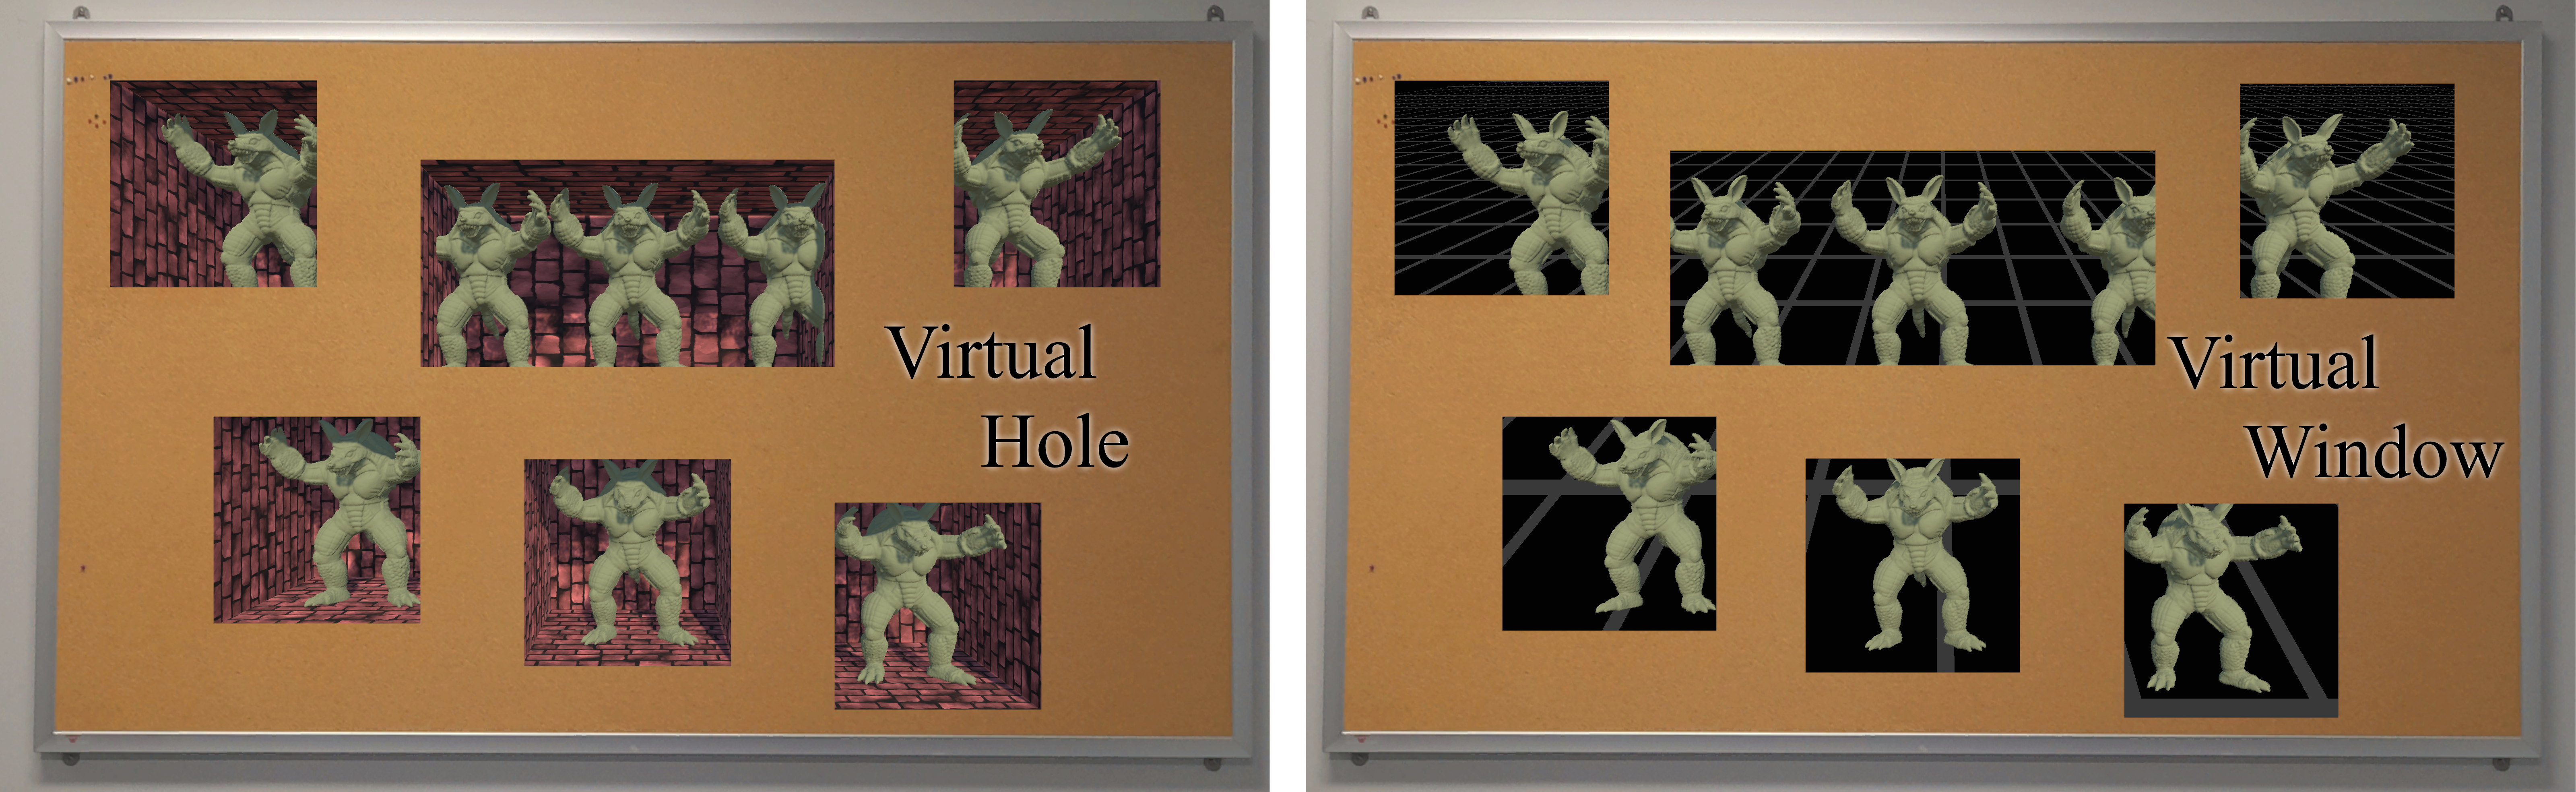
\includegraphics[width=\columnwidth]{Chapter2/Images/VirtualHoleAndVirtualWindowExamples.png}
    \caption[Armadillos sitting behind a corkboard in \gls{ar} with the same orientation using hole-in-the-worlds effects to function.]{Armadillos sitting behind a corkboard in \gls{ar} with the same orientation using hole-in-the-worlds effects to function. On the left are virtual holes, and on the right are virtual windows. }
    \label{fig:VirtualHoleAndVirtualWindowExamples}
\end{figure}

Although hole-in-the-world visualizations work quite effectively utilizing any \gls{ar} display~\cite{Bajura1992, DePaolis2019, Feiner1992, Avery2009, Muthalif2022, Habert2015}, they have a few limitations. Firstly, the visualization needs to be in a static position. 
It cannot rotate or change size relative to the userΓÇÖs motions, so the hole should not react to the user's position. 
The user could choose to make the hole larger or smaller without breaking the effect. There is a limited field of view into the hole. 
Although the limited view creates the \gls{X-ray Vision} effect, it restricts the user's view of the data. 
One advantage of this \gls{X-ray Vision} method is that it can be viewed using any display.

\paragraph{Virtual Box/Hole:}

\begin{figure}[t]
    \centering
    \includegraphics[width=0.6\columnwidth]{Chapter2/Images/BajuraetalX-ray.png}
    \caption[A image of Bajura et al.'s~\cite{Bajura1992} \gls{X-ray Vision} technique.]{A image of Bajura et al.'s~\cite{Bajura1992} \gls{X-ray Vision} technique. Used with permission from ACM \textcopyright{} 1992. Permission to make digital or hard copies of all or part of this work for personal or classroom use is granted without fee, provided that copies are not made or distributed for profit or commercial advantage}
    \label{fig:BajuraetalX-ray}
\end{figure}

The Virtual hole \gls{X-ray Visualization} was the first type of \gls{X-ray Vision} to be implemented and was designed by Bajura et al.~\cite{Bajura1992} (seen in \autoref{fig:BajuraetalX-ray}). 
Who aimed to visualize a baby fetus inside of its mother's womb.
They accomplished this by presenting a box for the baby to be seen in, which would allow for some level of occlusion.
It is still one of the most used \glspl{X-ray Visualization} and is still being researched in modern studies due to their effectiveness and versatility~\cite{Blum2012, DePaolis2019, Phillips2021}. 
Virtual holes have been found to provide a relationship between virtual objects and the real world. 


Research has also observed that introducing some particle occlusion alone may aid depth perception~\cite{Kyto2013}.
It has been observed by Kyt├╢ et al.~\cite{Kyto2013} that users could better determine distance if they had a partially occluded object in the scene for users to use as a reference or even using other virtual objects as a reference.
This was demonstrated in a study that partially occluded the edges of other objects and found that as long as some of the \gls{X-ray Vision} effects were covering part of the virtual scene, then it was possible to make smaller objects behind it appear to be a given depth behind as there was another object sitting in the front\cite{Kyto2013}.

\begin{figure}[tb]
    \centering
    \includegraphics[width=\columnwidth]{Chapter2/Images/AvvedutoEtAl.png}
    \caption[This image contains the \gls{X-ray Vision} study environment from Avveduto et al.~\cite{Avveduto2017}.]{This image contains the \gls{X-ray Vision} study environment from Avveduto et al.~\cite{Avveduto2017}. 
    a) shows a study setup that was utilized throughout this study, with the virtual objects present.
    b) shows the no \gls{X-ray Vision} condition used for this experiment from the participant's view.
    c) shows the \gls{X-ray Vision} conditions used for this experiment from the participant's view. 
    Used with Permission from Avveduto et al.~\cite{Avveduto2017}.
    }
    \label{fig:AvvedutoEtAl}
\end{figure}

\gls{sar} \gls{X-ray Vision} techniques papers utilize virtual holes as they work well with \gls{perspective_corrected_projection}~\cite{Avveduto2017, Heinrich2019, Heinrich2022}. 
The initial research in this space looks at what is required for a \gls{sar} based \gls{X-ray Vision} system. 
This was done by Avveduto et al.~\cite{Avveduto2017}, who asked participants to perform a mock biopsy like the one shown in \autoref{fig:AvvedutoEtAl}. 
Participants were then asked to attempt this procedure using either an image of a leathery surface or an image of buttons, which provided two different levels of contrast as backdrops for the virtual hole.
A virtual hole to a virtual hole with an occlusion mask against a baseline.
The authors found that using the occlusion mask and the virtual hole provided accurate results, with participants only being off by approximately 2.5cm (sd = 0.5), whereas in tasks where the participants used no \gls{X-ray Vision} 3cm (sd = 0.5). 


Heinrich et al.~\cite{Heinrich2019} later used virtual holes with \gls{sar} using \gls{perspective_corrected_projection} tested methods to illustrate depth perception with and without stereo vision. 
They compared using the conditions shown in \autoref{fig:Heinrich2019} (Phong Shading, Virtual Mirror, Depth-Encoding Silhouettes, Pseudo-Chromadepth, and Supporting Lines). 
This task asked participants to correctly identify the depth order of the cubes that can be seen in \autoref{fig:Heinrich2019}. 
This research found that the stereoscopic representation of SAR improved all conditions regarding time required and perceived difficulty. 
Pseudo-Chromadepth and Support Lines were the most effective \glspl{X-ray Visualization}, whereas Phong and the Virtual Mirror conditions were the most challenging. 

\paragraph{Cutaways and Tunnelling:}

\begin{figure}[!b]
    \centering
    \includegraphics[width=\columnwidth]{Chapter2/Images/ImagesFromOtherWorks/Heinrich2019.jpg}
    \caption[The conditions used in Heinrich et al.'s~\cite{Heinrich2019} investigation in to \gls{sar} based virtual holes.]{The conditions used in Heinrich et al.'s~\cite{Heinrich2019} investigation in to \gls{sar} based virtual holes. a) Phong Shading. b) Virtual Mirror. c) Depth-Encoding Silhouettes. d) Pseudo-Chromadepth. e) Supporting Lines. Used with permission from IEEE \textcopyright{} 2019.}
    \label{fig:Heinrich2019}
\end{figure}

Cutaways and Tunnelling present a hole through an object, revealing an object on the other side of the object~\cite{Avery2008, Avery2009, Feiner1992}. 
Both these techniques can be seen in \autoref{fig:JustTunneling}. They appear as a box with no back. 
The point of these visualizations is to give the sense of going through a real-world object.
These visualizations focus more on indicating where the data is in the real world rather than giving the user a better sense of depth when looking through a particular piece of data~\cite{Avery2009}.


Avery et al.~\cite{Avery2009} observed a slight offset to the perception of depth when tunneling is used on its own~\cite{Avery2009}. 
This can be improved by combining this technique with either a real-world overlay~\cite{Lerotic2007} or any Computer Vision-Enabled Technique~\cite{Avery2009} on either the front or back to help ground the visualization.
This allowed Avery et al.~\cite{Avery2009} and Lerotic et al.~\cite{Lerotic2007} to give their users the perspective of looking through a wall, whereas~\cite{Erat2018} used a smaller form of this to look through an individual wall. This smaller attempt would be considered a cutaway~\cite{Feiner1992}. 

Cutaways don't appear much in \gls{ar} literature however some notable works exist~\cite{Zollmann2012}. The smaller size of the effect means they may require another visualization to repair the depth offset. However, no research has been done to test whether this could be an issue.
Research from Erat et al.~\cite{Erat2018} did find that cutaways make for a very natural way to look through a wall to interact with something like a drone on the other side when compared to looking at the drone from a first-person's viewpoint, but little else is understood about using cutaways in \gls{ar} for \gls{X-ray Vision}.
When testing this use case, they found that technological limitations still held users back from utilizing \gls{X-ray Vision} to render objects underneath the ground~\cite{Erat2018}.

\begin{figure}[tb]
    \centering
    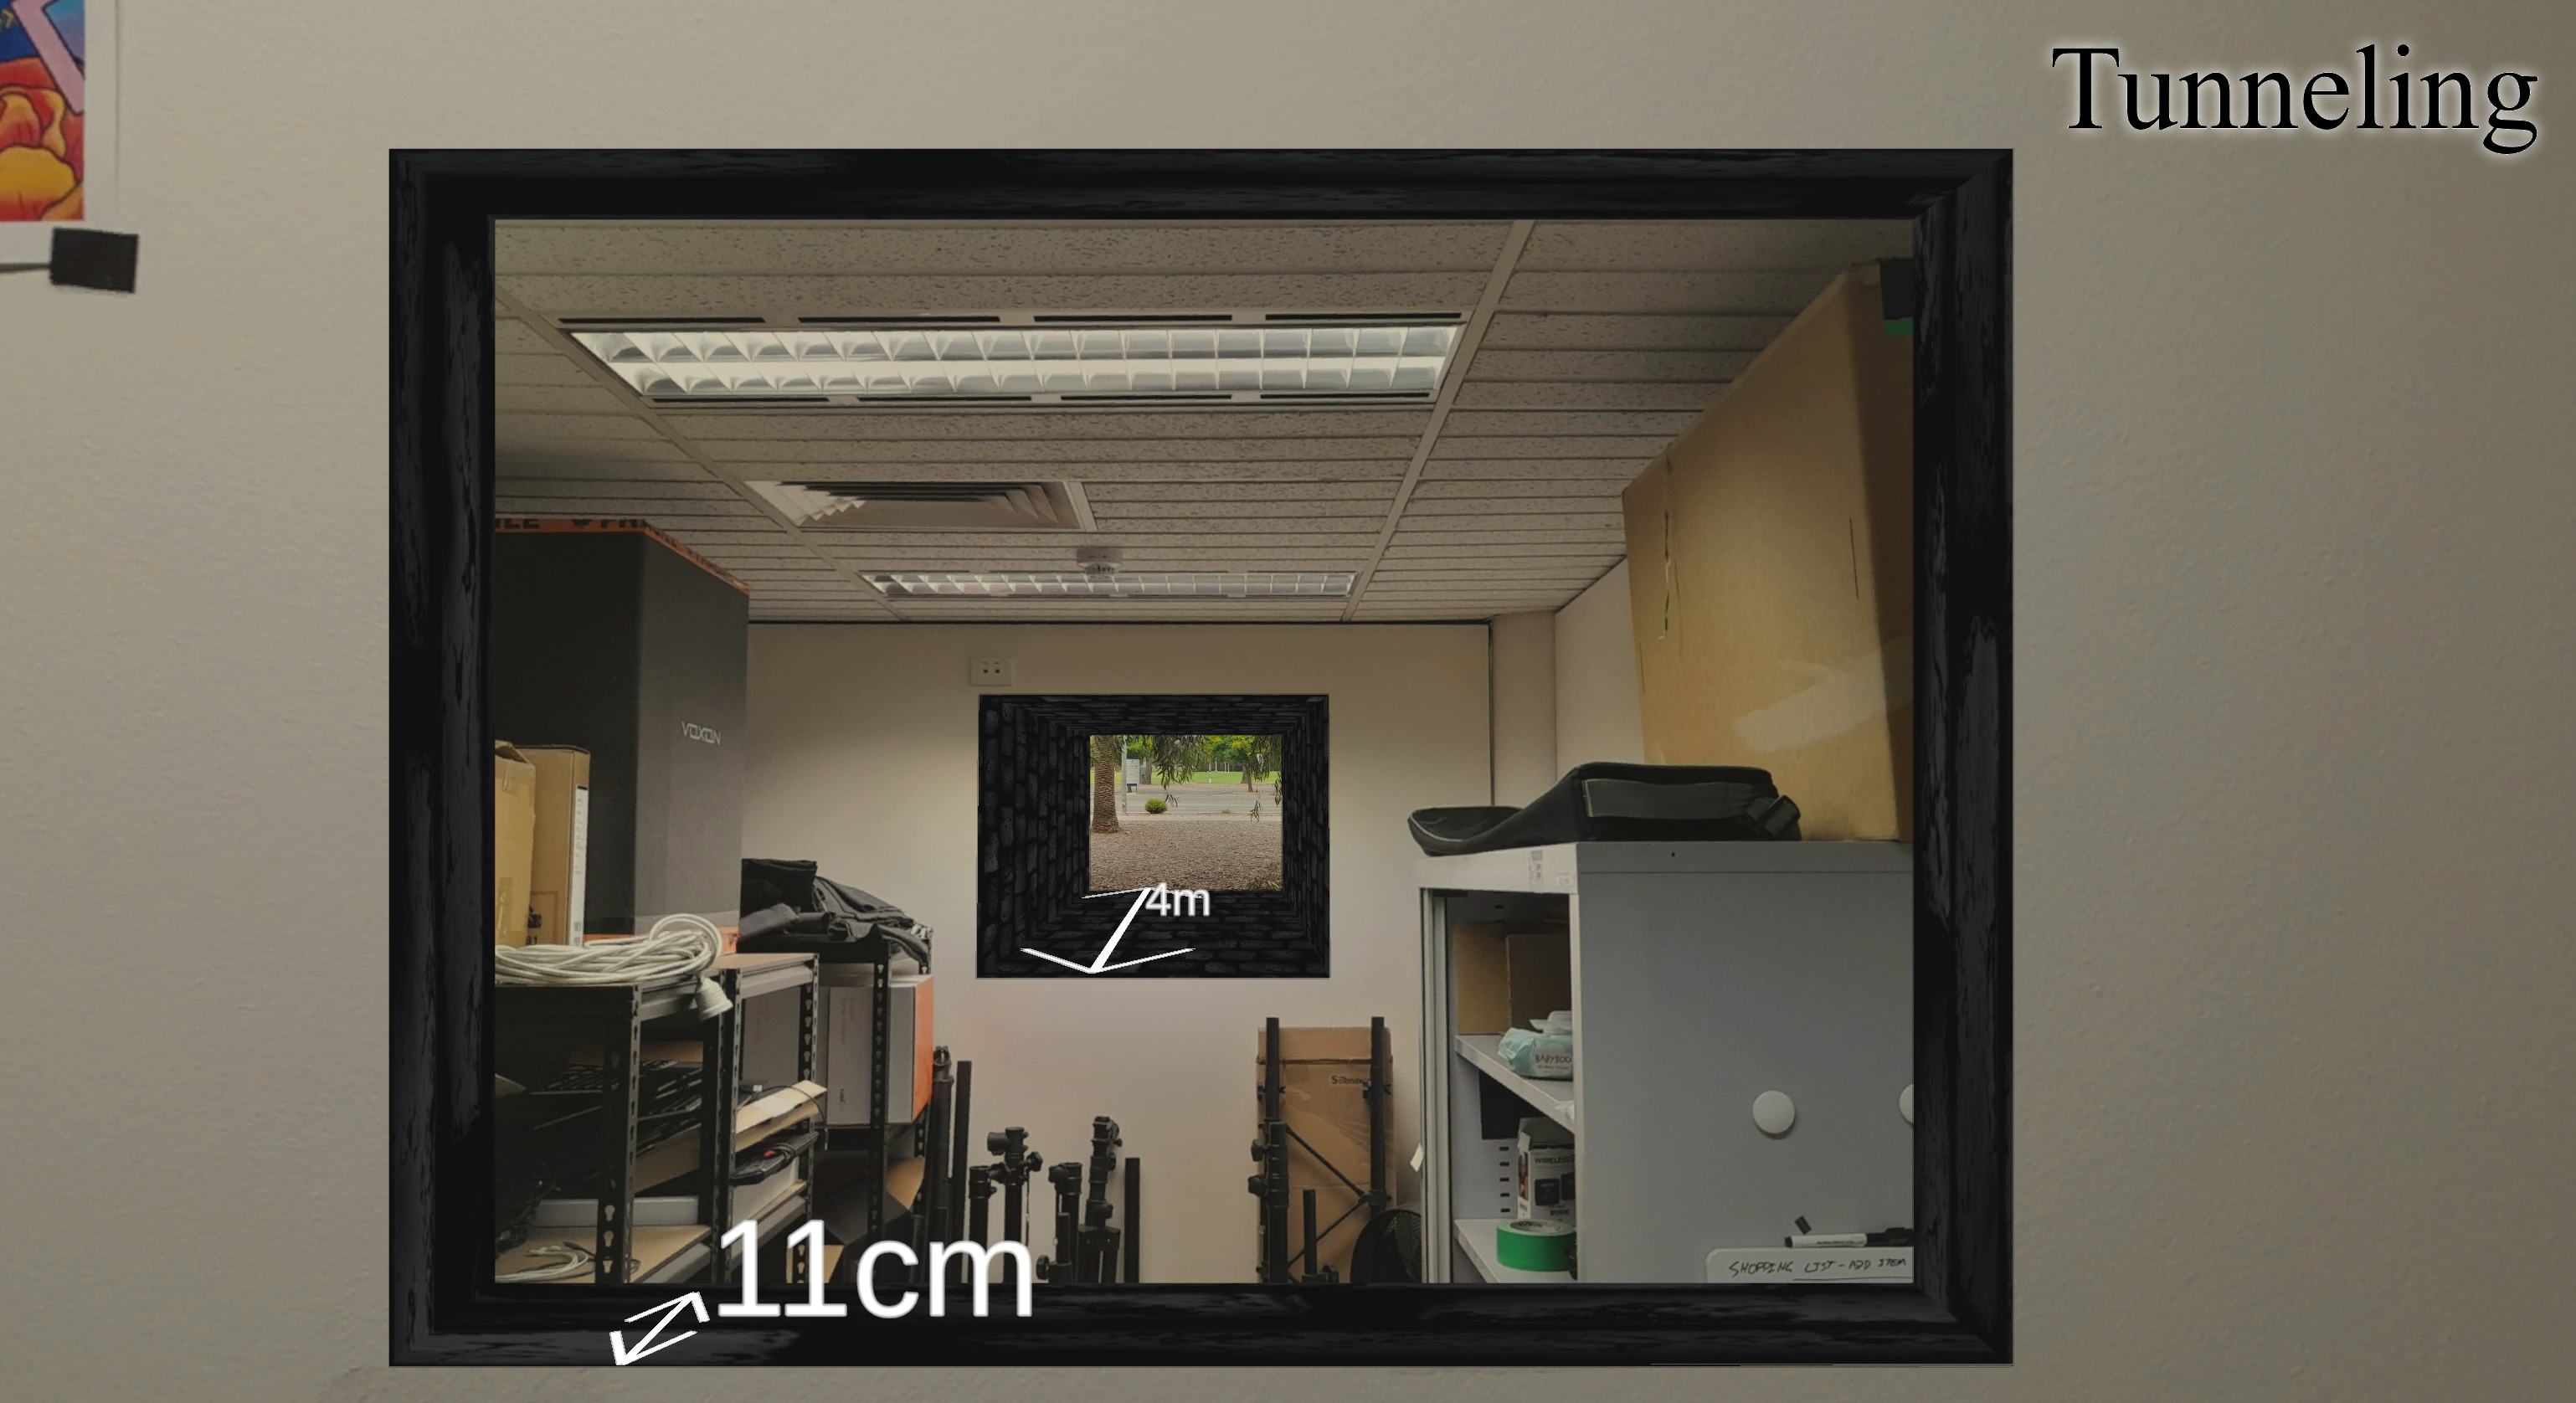
\includegraphics[width=\columnwidth]{Chapter2/Images/JustTunneling.png}
    \caption[A image of the tunneling x-ray visualization used to look through multiple walls.]{A image of the tunneling x-ray visualization used to look through multiple walls. The first arrow looks into a storeroom, whereas the second arrow looks out to the outside. White arrows showcase the depth of the tunnel.}
    \label{fig:JustTunneling}
\end{figure}

\paragraph{Virtual Windows:} 
Virtual Windows shows the user a perspective of a 2D hole in the wall. 
These are sometimes presented as a crack in the wall~\cite{Feiner1992} or will have a slight frame, but what separates this visualization from cutaways is that they ignore the content that is not known and start the virtual space immediately after the real-world surface~\cite{Phillips2022}.
This can be seen in \autoref{fig:VirtualHoleAndVirtualWindowExamples} , merging with the surface of a given material~\cite{Bichlmeier2007, Guo2022}. 

Guo et al.~\cite{Guo2022} utilized virtual holes to enable video games to take place in a \gls{non_euclidean_space}. 
The authors aimed to look at methods where \gls{X-ray Vision} could be made to be more interactive. 
Enabling people to play a game together regardless of their spatial requirements. 
Their experiment had them tag virtual objects that were to tag objects behind the physical walls, which showed to be almost as useful as giving the participants a virtual mini-map with the targets located on it.

Another form of \DIFdelbegin \DIFdel{virual }\DIFdelend \DIFaddbegin \DIFadd{visual }\DIFaddend windows has been titled "Contextual Anatomic Mimesis" by Bichlmeier et al.~\cite{Bichlmeier2007}. This is one of these windows designed to work autonomously with medical applications. 
The technique that blends virtual anatomical structures with the appearance of real tissue, gradually transitioning from realistic skin to virtual content.
It gradually moves from having the appearance of skin to looking more like the virtual content while still presenting a slight overlay based on the roughness of the skin~\cite{Bichlmeier2007}. 
The effects of Contextual Anatomic Mimesis were furthered by Martin-Gomez et al.~\cite{Martin-Gomez2021}, who have shown a significant improvement when paired with a another second effect to help represent the depth of an object.
Noting that using more than 1 depth cue is beneficial.
These effects ranged from hatching to applying shading to show shadows to the effect where it was found that hatching outperformed the other conditions (hole, ghosted mask, constant, shaded, black, chromatic, and bright)~\cite{Martin-Gomez2021}.
These results have led us to the understanding that illustrative effects may have a slight advantage when providing an understanding of the positioning of data for medical diagrams as they can not only provide a sense of depth perception but are also easy to understand for a general user. 

\subsubsection{Real-World Overlays} \label{sec:realWorldOverlay}
Another way of providing \gls{X-ray Vision} effects is to represent the physical environment using a virtual pattern such as a wireframe or a grid. 
This is typically done in two ways. One way is to place a pattern on the ground, allowing users to retain some knowledge of depth by using a constant geometric cue~\cite{Gruenefeld2020}. The other method utilizes overlaying the real-world object with a pattern of some sort. 
The second method is used when viewing virtual objects in stereoscopic displays, as it requires a level of geometric saliency to be perceptible. 
Binocular disparities are required for these types of visualizations to function~\cite{Otsuki2015}.

\begin{figure}
    \centering
    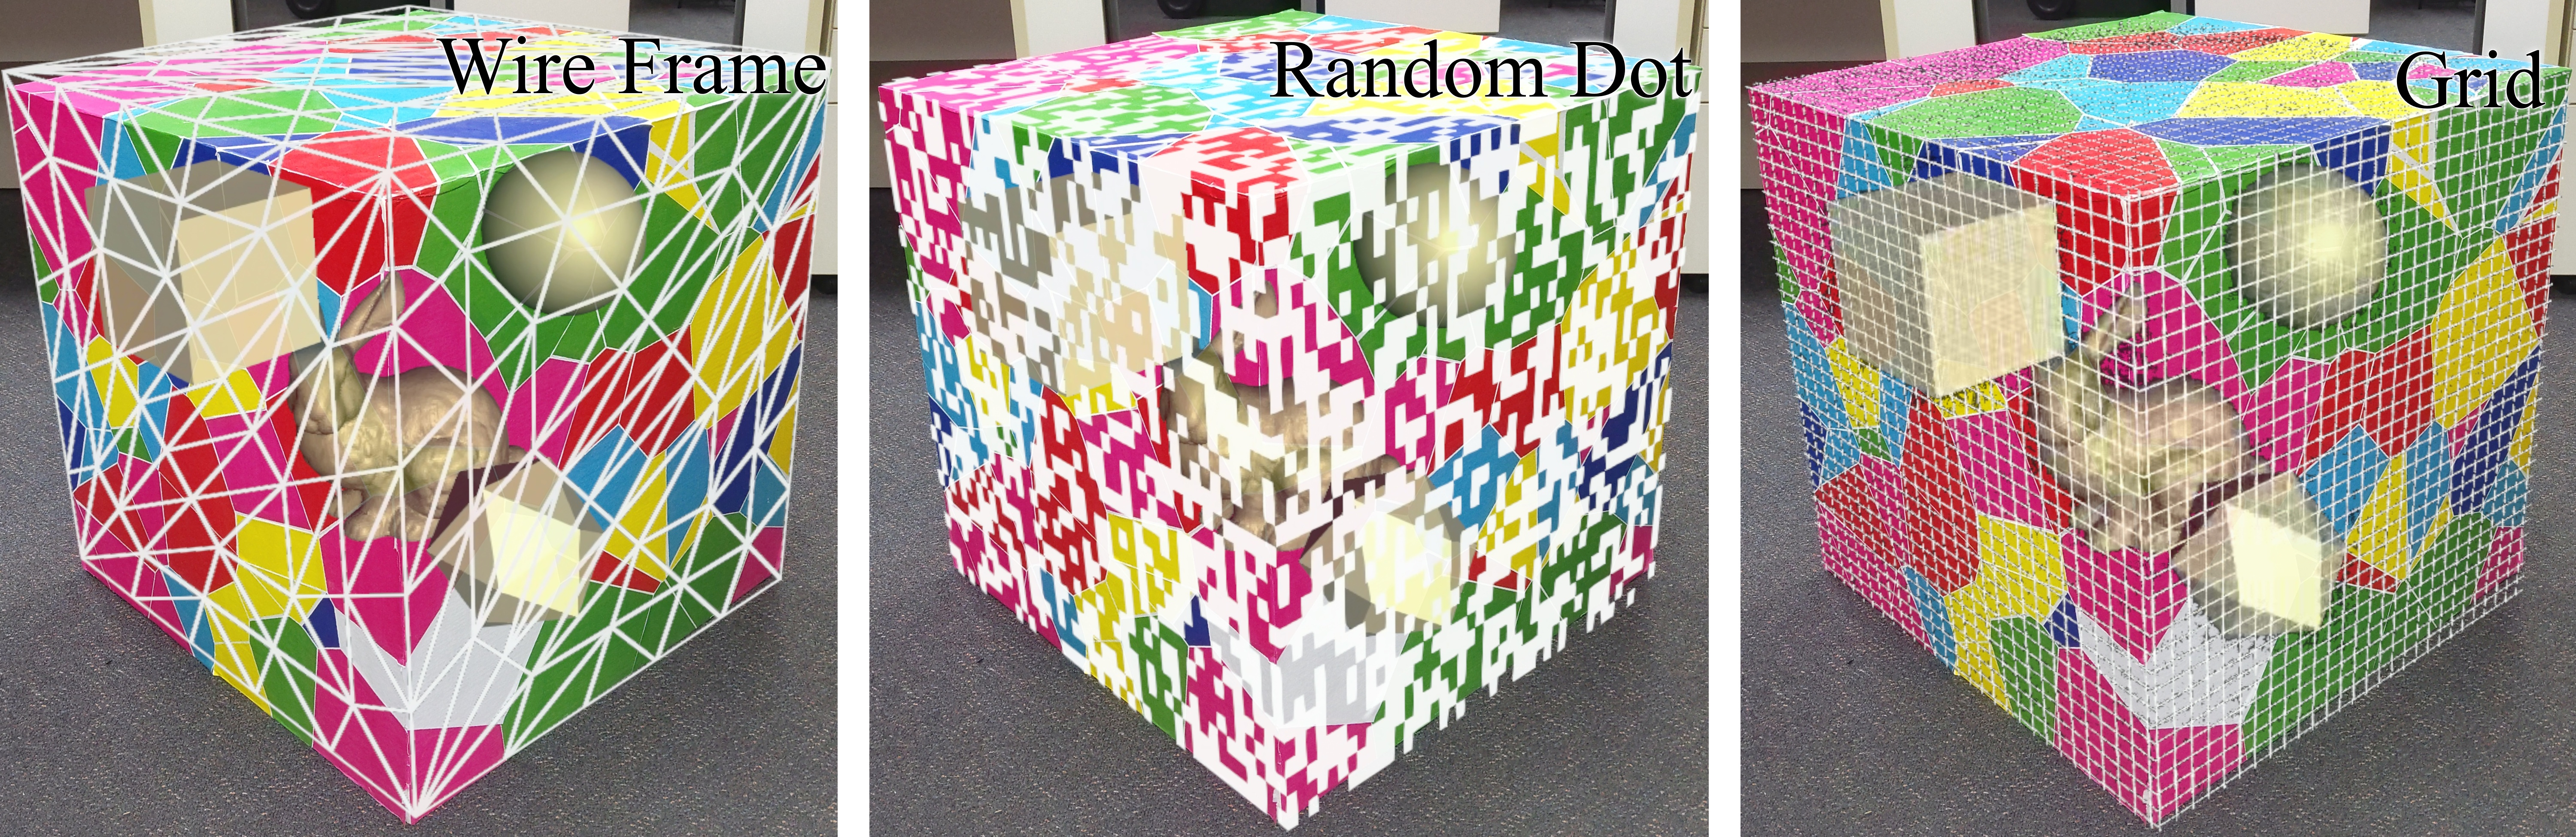
\includegraphics[width=\columnwidth]{Chapter2/Images/RealWorldOverlays.jpg}
    \caption[Wireframe, Random Dot, and Grid \gls{X-ray Visualization} over colorful patterned box with a virtual cube, sphere icosahedron, and a Stanford bunny rendered inside.]{This is a demonstration of real world overlay's and how they are \DIFdelbeginFL \DIFdelFL{utalized }\DIFdelendFL \DIFaddbeginFL \DIFaddFL{utilized }\DIFaddendFL as forms of X-ray vision. the \glspl{X-ray Visualization} Wireframe, Random Dot, and Grid and are placed over colorful patterned box with a virtual cube, sphere icosahedron, and a Stanford bunny rendered inside. The image was taken using the HoloLens' screen view. }
    \label{fig:RealWorldOverlays}
\end{figure}

Overlaying a real-world overlay as a guide over the ground does not require any specific device since as long as the overlay is able to interact with the real world environment. 
It will perform better, however, when it is used with a binocular \gls{hmd} as this can better represent the surface~\cite{Otsuki2016}.
While they do provide a good occlusive cue, the main role they serve is to help the user locate the position of an object with reference to a real world object. 
The additional cues provided from that point moving forward should take note of what is required from that point moving forward. 

\autoref{fig:RealWorldOverlays} illustrates forms real-world overlays can take, for example overlaying grids~\cite{Becher2021, Heinrich2022, Heinrich2019, Johnson2014}, Wireframes~\cite{Chen2020, Gruenefeld2020, Tsuda2005} and Random Dots~\cite{Ghasemi2018, Otsuki2015, Otsuki2016, Otsuki2017}. All of these effects are designed to utilize partial occlusion to highlight the shape of the object and to help the user understand the orientation of the wall. This gives the user a better comprehension of the distance between themselves and the objects they are looking inside of. 

\paragraph{Grids:}
Grids allow for a persistent barrier between a given surface and provide a guide on where a surface is in an augmented world~\cite{Johnson2014, Heinrich2022}. 
Johnson et al.~\cite{Johnson2014} developed a surgical system that utilized a grid-based visualization to allow for \gls{ct} data to be viewed at the correct position within the patient when using a wearing an \gls{ar} \gls{hmd}.
A grid was utilized to represent different types of flesh and a 3D object. 
They had surgical students utilize this system with laparoscopic video to evaluate it, where it was received with a positive reception from the subjective study which was conducted~\cite{Johnson2014}. 

\begin{figure}
    \centering
    \includegraphics[width=\columnwidth]{Chapter2/Images/ImagesFromOtherWorks/Heinrich2022.png}
    \caption[The conditions utilized for Heinrich et al.'s~\cite{Heinrich2022}  research.]{The conditions utilized for Heinrich et al.'s~\cite{Heinrich2022} research. The first row shows how they were visualized using the HoloLens, while the second line shows the output from the \gls{sar} display. The columns represent the three visualizations they used in their study, which were then split into three, showing the difference between their visualizations for guiding the angle and depth required for the needle. Used with permission from IEEE \textcopyright{} 2022.}
    \label{fig:Heinrich2022}
\end{figure}

Grids also tend to be utilized to explain to the user where the background of the \gls{X-ray Visualization} can be seen. 
\autoref{fig:Heinrich2022} shows how Heinrich et al.~\cite{Heinrich2022} utilized a grid overlaying a virtual hole and tested how accurate a biopsy would be using this as visualizations between an \gls{ost} \gls{ar} and \gls{sar}. 
This required testing the accuracy of the initial insertion angle and the depth to which the user placed the device. 
Heinrich et al.~\cite{Heinrich2022} utilized two conditions without \gls{X-ray Visualization}. 
One was a target that showed and would change in color when the needle approached the target, and the other was a virtual needle for the users to match. 
This method demonstrated that the glyph visualization was more effective than the \gls{X-ray Visualization}, as it provided participants with a more intuitive \gls{X-ray Vision} \DIFdelbegin \DIFdel{experiance}\DIFdelend \DIFaddbegin \DIFadd{experience}\DIFaddend .
However, both of them performed better than showing the visualization of the desired entry of the needle~\cite{Heinrich2022}. 

\paragraph{Random Dot:}
Random dot is another way of expressing more occlusion than other geometric pattern effects typically employed~\cite{Ghasemi2018, Otsuki2015}. This effect provides a partial sense of occlusion by providing a semi-occlusive layer over real-world objects~\cite{Otsuki2015}. 
This effect is one of the least computationally expensive but requires an immersive environment with flat surfaces. 
Highlighting various pixels on the surface of objects provides a stereoscopic effect of occlusion for the user and should technically allow for a better sense of depth. 

Ghasemi et al.~\cite{Ghasemi2018} conducted two studies to evaluate Random Dot visualizations. A psycho-physical depth perception experiment, which consisted of a series of thin circles, was run to determine the effectiveness of this \gls{X-ray Visualization}. 
Participants were given six different distances that ranged from 5mm in front and behind the visualization/wall.
The results study found that this effect is most effective when around 50\% of the space is filled using a random dot.
The amount of dots and their size could be altered, but it was most effective when more small dots were used up close and fewer larger ones up close and more remote. 
This distance could be increased if objects are further away from the wall, allowing for more depth perception. 

\paragraph{Halo and the Silhouette:}

\begin{figure}[t]
    \centering
    \includegraphics[width=\linewidth]{Chapter2/Images/OzgurEtAl.png}
    \caption[Ozgur et al.'s~\cite{Ozgur2017} \gls{X-ray Vision} system using Halos.]{
    Ozgur et al.'s~\cite{Ozgur2017} \gls{X-ray Vision} system using Halos.
    The silhouettes are generated through orthographic projection onto the front and back planes, which are oriented based on the sight line passing through the tumor's center of mass. These planes are positioned at the points where the organ's surface intersects the sight line.
    Used with permission from IEEE \textcopyright{} 2017 and Ozgur et al.~\cite{Ozgur2017}
    }
    \label{fig:JustHalo}
\end{figure}

This effect goes by many names but is most commonly called Halo or Silhouette as it creates an outline of the virtual objects.
It will be referred to as the Halo visualization in this dissertation for simplicity.
The Halo \glspl{X-ray Visualization} as stated in Ozgur et al.'s~\cite{Ozgur2017} paper presents the effect as a bright light around the edges of the object of interest and use alpha blending to communicate depth~\cite{Ozgur2017}. 
This effect is very similar to what is referred to as the "silhouette" effect in medical visualization~\cite{Rheingans2001}. 
However, terminology varies across fields, and in this thesis, I will consistently use the term "Halo visualization" to describe this effect for clarity. 
\autoref{fig:JustHalo} show how the the halo is set to leverage the depth perception cue of relative size.
This \gls{X-ray Vision} effect is unique due to its lack of occlusion, making it effective for surgical situations~\cite{Ozgur2017}. 
It has been tested using a monoscopic display in a study designed for minimally invasive surgeries. It can also exploit a color-based effect, applying visual language to communicate depth to the user~\cite{Ozgur2017}.

\subsubsection{Computer Vision-Enabled Techniques} \label{sec:ComputerVisionEnabledTechnqiue}
In computer vision, several methods are used to highlight salient features in an image. This is normally done by highlighting various salient factors within an image. 
These techniques are commonly used on monoscopic \gls{vst} devices as they provide a good sense of where an object is positioned relative to another in 2D. 
This is separate from the Halo technique as these do not generally \DIFdelbegin \DIFdel{utalize }\DIFdelend \DIFaddbegin \DIFadd{utilize }\DIFaddend the image of the real world while the halo technique \DIFdelbegin \DIFdel{utalizes }\DIFdelend \DIFaddbegin \DIFadd{utilizes }\DIFaddend the shape of the object that has been inserted. 
To this date, the results lack the performance of Computer Vision-Enabled Techniques in stereo, with most of the publications found in this space either being demos or research proposals~\cite{Rompapas2014, Phillips2021}.

\begin{figure}[!b]
    \centering
    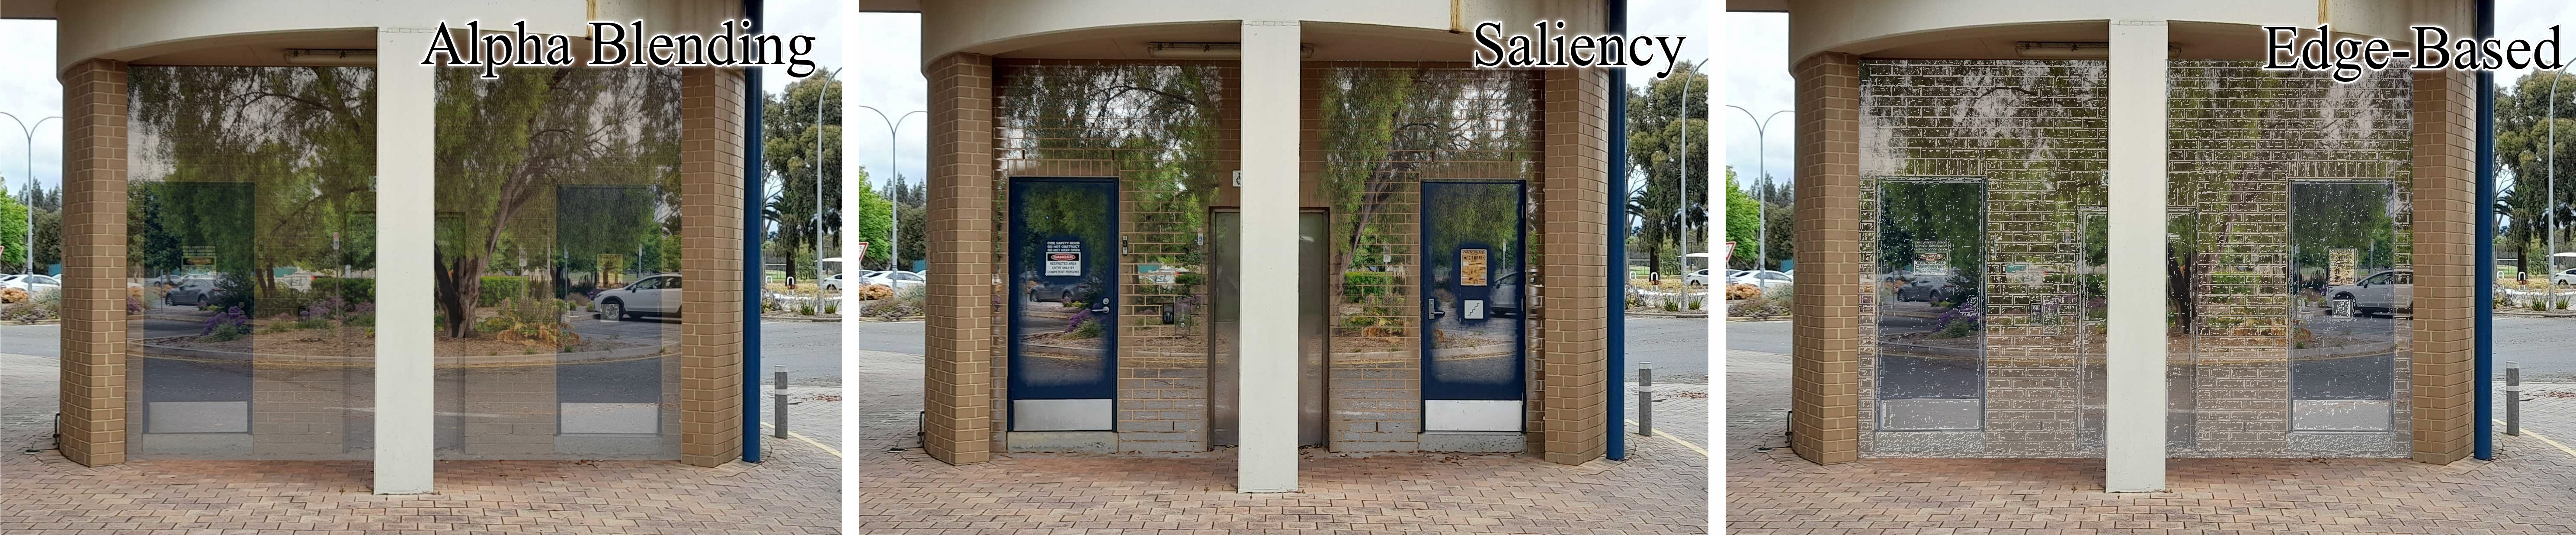
\includegraphics[width=\columnwidth]{Chapter2/Images/ComputerVisionEffectsAndTransperency.jpg}
    \caption{\gls{X-ray Vision} showing alpha blending, Saliency, and edge-based Visualizations (Shown left to right) looking through a building.}
    \label{fig:ComputerVisionEffectsAndTransperency}
\end{figure}

\paragraph{Edge-Based:}
Edge-based \glspl{X-ray Visualization} (depicted in \autoref{fig:ComputerVisionEffectsAndTransperency}) identify areas in the userΓÇÖs view that contrast highly between neighboring pixels and highlight them. 
This high contrast effect tends to be regarded by most humans as salient, making it a reliable method for determining salient artifacts~\cite{Avery2009}. 
Created initially by Kalkofen et al.~\cite{Kalkofen2007} to allow for better image-based \gls{X-ray Vision}.
This visualization creates a predictable method for highlighting areas on an image (given that the surface has a high level of contrast) and makes it a popular way of showcasing \gls{X-ray Vision} on a monoscopic \gls{ar} device~\cite{Avery2009, Chen2010, Kalkofen2007, Sandor2010}. 
By highlighting the visible edges of an object, it is possible to create the appearance that an object is behind the object either through partial occlusion~\cite{Avery2009, Kalkofen2007} or by cutting out elements of the X-rayed object~\cite{Dey2012, Dey2014}.

\paragraph{Saliency:}
Saliency highlights areas of the real world that are likely to be of interest and makes the areas that are unlikely to be less apparent. 
\autoref{fig:ComputerVisionEffectsAndTransperency} shows one method of using saliency as an \gls{X-ray Visualization}. 
The visualization technique can vary between implementations because it can be done algorithmically~\cite{Sandor2010} or by training an AI model to detect the features a human is more or less likely to look at~\cite{Cong2019}. 
A user could naturally peer through objects using the saliency method, given that the camera could find some salient and non-salient areas of the image~\cite{Sandor2010}. 
As of the beginning of this thesis, Saliency has only been utilized with \gls{vst} \gls{ar}.

\paragraph{Ghosting:}
Ghosting utilizes the effects of visual saliency and focuses on allowing artistic approaches to partial occlusion~\cite{1238308, Zollmann2010}. Adaptive Ghosting is an extension that combines the salient effect of ghosting and edge-based \gls{X-ray Vision} effects. 

\begin{figure}[tb]
    \centering
    \includegraphics[width=1\linewidth]{Chapter2/Images/KalkofenEtAlSystem.png}
    \caption[A description of the \gls{X-ray Vision} system used by Kalkofen et al.~\cite{Kalkofen2013}]{A description of the \gls{X-ray Vision} system used by Kalkofen et al.~\cite{Kalkofen2013}. This image shows the various components of the graphics pipeline \DIFdelbeginFL \DIFdelFL{requried }\DIFdelendFL \DIFaddbeginFL \DIFaddFL{required }\DIFaddendFL to create the adaptive ghosting effect.
    (a) The occluder and occluded elements are combined into a ghosted view using state-of-the-art transparency mapping based on the importance map of the occluder. However, this initial ghosted view lacks is difficult to \DIFdelbeginFL \DIFdelFL{intergrate }\DIFdelendFL \DIFaddbeginFL \DIFaddFL{integrate }\DIFaddendFL into the real world seamlessly as it is either used to cover a area or it is not. To address this, a new importance map is generated for the resulting ghosted view which looks at area's of high contrast and places the \DIFdelbeginFL \DIFdelFL{visulisation }\DIFdelendFL \DIFaddbeginFL \DIFaddFL{visualisation }\DIFaddendFL on to them as well as over the rest of any are's close to virtual elements that need to be seen within the physical objects.
    (b) This new importance map is then compared to the original importance map of the occluder. Features that were marked as important in the occluder but are no longer prominent in the ghosted view are identified for enhancement.
    (c) By applying these enhancements to the adaptive ghosted view, the previously obscured important structures become clearly visible again.
    Used with permission from IEEE \textcopyright{} 2013.
    }
    \label{fig:KalkofenEtAlSystem}
\end{figure}

Zollman et al.~\cite{Zollmann2014} tested the effectiveness of Edge-Based, Ghosting, and Randomly occluding underground pipes.
Participants were asked to identify the depth of the pipes, which were located underground, based on a series of Images they received.
This study found that ghosting was better equipped than edge-based \gls{X-ray Vision} at identifying depth underground and noted that it was easy to use, but it did observe the details of the shape. 

Adaptive Ghosting technique to the current environment makes it less varied when viewing it from different directions~\cite{Kalkofen2013}.
\autoref{fig:KalkofenEtAlSystem} presents Kalkofen et al.'s~\cite{Kalkofen2013} system for Adaptive Ghosting, which normalizes the contrast of the input image to allow this effect to maintain a similar effect even in different lighting. 
This system combats one major issue with computer vision-enabled \gls{X-ray Vision} techniques: their inconsistency depending on changes to the scene and lighting. 
Adaptive Ghosting can cause unexpected artifacts and misleading visualizations, but it is still possible to notice this effect even when using Adaptive Ghosting.

\subsubsection{Comparisons Of X-ray Vision Effects}


\begin{figure}[tb]
    \centering
\includegraphics[width=\columnwidth]{Chapter2/Images/ComparisionsOFVisionInTheLiturature.pdf}
    \caption[A heat map illustrating how often different \gls{X-ray Vision} effects are compared to each other in the literature.]{
        A heat map illustrating how often different \gls{X-ray Vision} effects are compared to each other in the literature. The diagonal cells (from lower left to upper right) show the total number of studies for each effect, while the center row indicates studies that examined each effect individually without comparison.

}
    \label{fig:ComparisionsOFVisionInTheLiturature}
\end{figure}

Given all these methods of \gls{X-ray Vision}, it is quite common for people to try to compare them to determine the positive and negative aspects. 
Studies in this area have investigated:
\begin{itemize}
    \item The amount of occlusion density required for visualizations to create the \gls{X-ray Vision} \DIFdelbegin \DIFdel{visulisations  }\DIFdelend \DIFaddbegin \DIFadd{visualisations  }\DIFaddend and effective limits to the practicality of these effects~\cite{Santos2016};
    \item How different displays react to \glspl{X-ray Visualization} on Mobile Devices~\cite{Dey2012, Dey2014}.
    \item What is the impact of \gls{X-ray Vision} between different visualizations~\cite{Sandor2010, Zollmann2014, Martin-Gomez2021, Gruenefeld2020}.
\end{itemize}
These comparisons are detailed in \autoref{fig:ComparisionsOFVisionInTheLiturature}.

Partial occlusion is important to most \glspl{X-ray Visualization}. It shows how much occlusion is needed for a given technique and how much occlusion makes interactions impossible.
This was the question that Santos et al.~\cite{Santos2016} addressed for mobile \gls{ar} \gls{X-ray Vision} when using edge-based or saliency \gls{X-ray Vision} effects.
This study had participants look at a box wrapped in either wrapping paper or crumpled foil.
This study utilized two tasks: One looking at what thresholds were required to allow participants to see 2D objects using \gls{X-ray Vision} effects, and the other looking at the maximum allowable alpha values these effects could have~\cite{Santos2016}. 

Santos et al.'s~\cite{Santos2016} first tested how the user could see four objects placed inside the box and asked them to reveal the maximum decision cutoff (threshold).
The next task was to lower the alpha value of the visualization until participants could clearly see the object hidden behind it. 
Inside the box would be visualized an image of an object they were asked to see, which could either be a small or a large object about the box. 
Each second, the transparency of the visualization would decrease, asking them to press a button on the display to stop the visualization when they could identify the item.
The combination of Santos et al.'s~\cite{Santos2016} results indicates the clarity of the object was dependent on the size, color, and texture of the box rather than the visualization used. 
The study noted Saliency was slightly harder to see through but not to a significant level. 
This dissertation treats these results as a guideline and has based its use of transparency and contrast with \gls{X-ray Vision} on these results. 

Sandor et al.~\cite{Sandor2010} Compared Edge-based visualizations to their newer Saliency visualization by having participants try to find a target in four scenes. 
This study found little difference between saliency and edge-based visualizations, but participants preferred the edge overlay. 
After this, both these conditions were tested using an online survey where participants would look at images presenting the information where saliency was seen to be better for providing \gls{X-ray Vision} for images. 

Dey et al.~\cite{Dey2012, Dey2014} compared \gls{X-ray Vision} on different-sized mobile devices to determine the display size could impact the visualizations required for Mobile devices.
Firstly, they developed an \gls{X-ray Visualization} called Melt, which showed a part of the foreground and a part of the background together.
Their first experiment tested the Edge-based technique against the Melt X-ray technique from far distances using a 7-inch display.
This study found that Melt was a more accurate in-depth estimation but took the participants longer to judge, which was likely used to overcome the drawbacks of the visualization~\cite{Dey2012, Dey2014}.

Dey et al.~\cite{Dey2014} ran a user study comparing Edge-based and Saliency using a Mobile \gls{ar} display. 
They created three levels of each \gls{X-ray Visualization}, where they were more or less sensitive to environmental concerns.
These results indicated that users struggled to use \gls{X-ray Visualization} when the edges were too thick for the edge-based variable, and saliency struggled in bright environments. 

All of the comparisons explained in this section utilized similar \gls{X-ray Vision} visualizations and most focused on how \glspl{X-ray Visualization} worked in different areas.
All these examples utilize mobile devices, so how these would affect \glspl{hmd} in general is a question that is yet to be answered. 
Also, most of these comparisons have utilized various forms of computer vision techniques (except for one use of the Melt visualization). 
Currently, there are many unknowns that exist in this space.


\subsection{Applications of X-ray Vision}

\begin{figure}[tb]
    \centering
    \includegraphics[width=\columnwidth]{Chapter2/Images/ImagesFromOtherWorks/Eren2018.png}
    \caption[Eren et al.'s~\cite{Eren2013} different visualizations of underground pipe networks using \gls{X-ray Vision} techniques.]{Eren et al.'s~\cite{Eren2013} different visualizations of underground pipe networks using \gls{X-ray Vision} techniques. a) baseline, b) edge-based, c) virtual hole, and d) cross-sectional techniques. Used with permission from Springer Nature \textcopyright{} 2018.}
    \label{fig:Eren2013}
\end{figure}

X-ray vision has been applied across a wide range of domains where visualizing hidden or internal structures is valuable. Medical research has been a central focus, where overlays of anatomical structures can support diagnosis and guide surgical procedures by allowing clinicians to perceive organs, tissues, and bones in situ~\cite{Bichlmeier2007, Blum2012, Bajura1992}. While demonstrations have shown promise, challenges remain around depth perception and real-time performance, as highlighted in comparative evaluations of iso-surfaces, direct volume rendering, and alternative rendering effects~\cite{Sielhorst2006, Bichlmeier2007}. Outside of medicine, construction and maintenance tasks also benefit, with researchers exploring techniques for seeing into walls or underground pipe networks. Early work by Feiner et al.~\cite{Feiner1995} focused on gradually revealing occluded structures, and more recent studies (e.g., Eren et al.~\cite{Eren2013,Eren2018}, shown in \autoref{fig:Eren2013}) have evaluated different visualization methods for accurately perceiving underground utilities.

Beyond these domains, X-ray vision concepts have been investigated in security, navigation, and education. In security, transparency effects and perspective-corrected projections have been used to augment situational awareness, though evaluations suggest togglable, more occlusive effects may be most effective~\cite{Kameda2004, Tsuda2005, Ohta2010}. Navigation and tourism applications demonstrate how seeing through structures or into the past can improve wayfinding and enrich cultural experiences, with evaluations showing reduced cognitive load compared to traditional maps~\cite{Dey2011, Maia2016, Yamamoto2014}. In education, while the effects of X-ray vision itself remain underexplored, augmented reality has been shown to increase engagement and may support long-term retention in domains like anatomy~\cite{Akpan2019, Santos2015}.

Entertainment provides a final but growing space for X-ray vision. While formal research is limited~\cite{Guo2023}, several commercial AR games such as MicrosoftΓÇÖs RoboRaid and Dr. Grordborts Invaders (shown in \autoref{fig:DrGrordbortsInvaders}) have experimented with the concept, using it to merge real and virtual environments in playful, interactive ways. These applications highlight both the versatility of X-ray vision across domains and the ongoing challenges of designing visualization techniques that are perceptually effective, intuitive, and computationally feasible.

\begin{figure}[tb]
    \centering
    \includegraphics[width=\columnwidth]{Chapter2/Images/ImagesFromOtherWorks/DrGrordbortsInvaders.jpg}
    \caption[A promotional Image from Dr Grordborts Invaders made by Weta Workshop for the Magic Leap.]{A promotional Image from Dr Grordborts Invaders made by Weta Workshop for the Magic Leap. Used with permission from Weta Workshop.}
    \label{fig:DrGrordbortsInvaders}
\end{figure}


\subsection{Hardware For X-ray Vision}
\glspl{X-ray Visualization} can be split into two key components to enable \gls{X-ray Vision}: A display to view the visualization and sensors to collect the data for \gls{X-ray Vision}.
While many studies have utilized collected information, allowing them to require only devices to collect pre-rendered devices, others have utilized a display. 


\glspl{X-ray Visualization} rely on two essential aspects: the availability of data representing the internal or hidden structures, and the means to visualize this data effectively. While many studies utilize pre-existing or independently collected datasets, others focus on the development and evaluation of display technologies for presenting \gls{X-ray Vision}. It is important to note that data acquisition is typically a separate process from visualization, and in most cases, data is gathered without a specific visualization method in mind.
However, the choice of data acquisition can limit the types of visualizations that can be effectively employed. For instance, real-time data acquisition methods may restrict the complexity of visualizations due to processing constraints, while pre-collected datasets allow for more intricate and computationally intensive visualization techniques.

\begin{figure}[tb]
    \centering
    \includegraphics[width=\columnwidth]{Chapter2/Images/DispalyModesUsedForXRayVis.png}
    \caption{A bar graph of the type of display used to visualize the various \gls{X-ray Vision} effects.}
    \label{fig:DispalyModesUsedForXRayVis}
\end{figure}

\subsubsection{Displays}
\gls{ar} displays come in different variations, each with its own benefits.
These different types of displays can be generalized as \gls{ost} \gls{ar}, \gls{vst} \gls{ar}, and \gls{sar}.
\gls{ost} \gls{ar} works by projecting the image on a transparent reflective display, creating a transparent display which is generally used for \glspl{hmd}.
\gls{vst} \gls{ar} displays utilize one or more cameras and display them with graphics overlaid on them. 
\gls{sar} uses projectors to place computer graphics to overlaid onto reality.
\autoref{fig:DispalyModesUsedForXRayVis} shows there are preferences between different types of \gls{X-ray Vision} devices to an extent due to the individual benefits and \DIFdelbegin \DIFdel{disbenefits }\DIFdelend \DIFaddbegin \DIFadd{drawbacks }\DIFaddend caused by these displays which have been laid out in \autoref{tab:XRayVisionDeviceComparison}.
\autoref{fig:ARTypesAndVisUsage}, shows real-world overlays are much more common than computer vision techniques, but real-world visual techniques are less common on monoscopic displays. 



\newlist{titemize}{itemize}{3}
\setlist[titemize,1]{label=--, left=0pt, itemsep=1pt, topsep=2pt, parsep=0pt}
\setlist[titemize,2]{label=$\ast$, left=1.5em, itemsep=1pt, topsep=1pt, parsep=0pt}
\setlist[titemize,3]{label=$\circ$, left=3em, itemsep=1pt, topsep=1pt, parsep=0pt}


\begin{table}[ht]
    \small
    \centering
    \caption{Advantages and Disadvantages of Devices Used for X-ray Vision}
    \label{tab:XRayVisionDeviceComparison}

\begin{tabular}{p{0.45\linewidth}|p{0.45\linewidth}}
        \hline
        \multicolumn{2}{c}{\textbf{OST AR Head-Mounted Displays (Optical See-Through)}} \\
        \hline
        \textbf{Advantages} & \textbf{Disadvantages} \\
        \hline
        \begin{titemize}
            \item Direct view of real world with overlays
            \item Maintains natural depth cues and peripheral vision
            \item Good for tasks needing situational awareness (e.g., surgery)
            \item Hands-free operation
        \end{titemize}
        &
        \begin{titemize}
            \item Limited brightness and contrast
            \item Smaller field of view vs. VST
            \item Alignment/calibration issues
            \item Optical distortion of virtual content
            \item Lower graphical fidelity
        \end{titemize} \\
    \end{tabular}
    \vspace{1em}

\begin{tabular}{p{0.45\linewidth}|p{0.45\linewidth}}
        \hline
        \multicolumn{2}{c}{\textbf{VST AR Head-Mounted Displays (Video See-Through)}} \\
        \hline
        \textbf{Advantages} & \textbf{Disadvantages} \\
        \hline
        \begin{titemize}
            \item High graphical fidelity and brightness
            \item Easier integration of computer vision
            \item Wider field of view possible
            \item Flexible virtual content manipulation
        \end{titemize}
        &
        \begin{titemize}
            \item Camera-mediated view
            \begin{titemize}
                \item Latency
                \item Distortion
            \end{titemize}
            \item Lower situational awareness
            \item Reduced situational awareness
            \item Can cause motion sickness
            \item Heavier, bulkier hardware
        \end{titemize} \\
    \end{tabular}
    \vspace{1em}

\begin{tabular}{p{0.45\linewidth}|p{0.45\linewidth}}
        \hline
        \multicolumn{2}{c}{\textbf{Mobile Devices (Phones/Tablets)}} \\
        \hline
        \textbf{Advantages} & \textbf{Disadvantages} \\
        \hline
        \begin{titemize}
            \item Widely available, easy to use
            \item Bright displays
            \item Portable for quick tasks
            \item Stable, high-quality graphics
        \end{titemize}
        &
        \begin{titemize}
            \item Less immersive
            \item Must be handheld
            \item Smaller screens limit detail
            \item Hardware fragmentation
            \item Limited spatial interaction
        \end{titemize} \\
    \end{tabular}
    \vspace{1em}

\begin{tabular}{p{0.45\linewidth}|p{0.45\linewidth}}
        \hline
        \multicolumn{2}{c}{\textbf{Spatial Augmented Reality (SAR) / Projectors}} \\
        \hline
        \textbf{Advantages} & \textbf{Disadvantages} \\
        \hline
        \begin{titemize}
            \item Projects info directly on objects
            \item Multiple users at once
            \item No wearables needed
            \item Limited multi-user suitability
        \end{titemize}
        &
        \begin{titemize}
            \item Needs precise calibration/tracking
            \item Works best in controlled environments
            \item Sensitive to lighting/surface
            \item Limited multi-user suitability
        \end{titemize} \\
    \end{tabular}
    \vspace{1em}

\begin{tabular}{p{0.45\linewidth}|p{0.45\linewidth}}
        \hline
        \multicolumn{2}{c}{\textbf{Desktop/Fixed Screens}} \\
        \hline
        \textbf{Advantages} & \textbf{Disadvantages} \\
        \hline
        \begin{titemize}
            \item High computational power
            \item Stable, high-quality graphics
            \item Large display for detail
            \item Comfortable for long use
            \item Good for collaboration
            \item Easy integration with systems
        \end{titemize}
        &
        \begin{titemize}
            \item Not immersive
            \item Stationary, low spatial interaction
            \item Requires looking away from real world
            \item Limited field of view
            \item Not mobile-friendly
        \end{titemize} \\
    \end{tabular}

\end{table}

\renewlist{titemize}{itemize}{1}
\setlist[titemize,1]{}




\gls{X-ray Vision} systems can be supported by display devices, including mobile phones, head-mounted displays, computer screens, and projectors~\cite{Kim2018}. Devices range from traditional computer screens and mobile personal devices, head-mounted displays to projectors. 
Most earlier devices only accommodate monocular vision, while recent head-mounted displays can support stereoscopic vision. \autoref{fig:LitRevewDeviceFrequencyPlot} shows that the choice of technology is often a result of technological advances and emerging products. It can be observed that mobile screen-based displays were most popular following the release of powerful mobile phones in 2007, underpinned by emerging computer vision techniques for tracking and the generation of visualizations. Similarly, stereoscopic head-mounted displays have gained popularity because of increased capabilities, technology maturity, and general availability in recent years.

Recently, research utilizing Microsoft HoloLens 1 and 2 has been widely used in \gls{X-ray Vision} research because of their advanced display tech and gesture recognition, making them a useful device for security and medical operations~\cite{Phillips2020, Martin-Gomez2021, Rodrigues2017, AlJanabi2020}. \glspl{hmd} shine in medical settings, offering a sterile work environment. Medical applications use screens for remote interactions, like controlling robotic arms in minimally invasive surgery~\cite{Kalia2019}. In contrast, the construction and maintenance industries employ diverse devices due to their varied environments~\cite{Muthalif2022, Eren2013, Eren2018, Becher2021}.

\begin{figure}[bt]
    \centering
    \includegraphics[width=\columnwidth]{Chapter2/Images/ARTypesAndVisUsage.png}
    \caption{A bar graph displaying The types of \gls{ar} that was used to visualize the different types of \gls{X-ray Vision} effects.}
    \label{fig:ARTypesAndVisUsage}
\end{figure}




\subsubsection{Comparison of Displays} \label{sec:ComparisionOfDisplays}
Comparing the effectiveness of different displays seems to be a relatively new area of study for \gls{ar} enabled \gls{X-ray Vision}.
Prior to starting this dissertation in 2019, our review found no studies that compared \glspl{X-ray Visualization} between different papers.
Since then, several studies have published their results on comparing \gls{vst} \gls{ar} devices against \gls{ost} \gls{ar} devices.

Gruenefeld et al.~\cite{Gruenefeld2020} performed depth perception studies using an OST headset utilizing \gls{X-ray Vision}, including Grid, Cut-out effects. 
The grid effect, placed on the ground within the X-ray able space and a perpendicular wall facing the viewer, could be used to approximate a relationship between the wall and the object. In contrast, the cut-out visualization provided a hole in the wall, which the user could look through to see where the object was on the other side, against a baseline that pointed participants to the object with a red arrow and displayed a perpendicular line going from the far point of the arrow to the bottom of the visualization. 
Gruenefeld et al.'s~\cite{Gruenefeld2020} found that the weakest of the depth cues were the cut-out. This was because the cues did not convey a clear depth indications to the user~\cite{Gruenefeld2020}, because the grid effect provided a clear indication of depth, allowing the users to count the amount of grid squares between the object and the wall they had a better sense of depth.

Another set of studies published by Martin-Gomez et al.~\cite{MartinGomez2021} studied the difference between four \glspl{X-ray Visualization} (None (Superimposition), virtual hole, ghosting, and Random Dot) on both \gls{vst} \gls{ar} and \gls{ost} \gls{ar} devices in the near field. 
They found that users better utilized \gls{X-ray Vision} on a \gls{vst} \gls{ar} headset than on an \gls{ost} \gls{ar} device.
This prompted another study investigating different rendering techniques for \gls{X-ray Vision} (shading, hatching, ghosting) and brightness levels, finding that bright, clear objects work best in \gls{ost} \gls{ar}.

Heinrich et al.'s~\cite{Heinrich2022} research comparing \gls{ost} \gls{ar} displays to \gls{sar} displays (previously mentioned in \autoref{sec:realWorldOverlay}) presented findings that both \gls{ost} \gls{ar} and \gls{sar} displays functioned in a similar fashion. 
However, they found that \gls{X-ray Vision} works better with \gls{ost} \gls{ar} displays, while \gls{ui} elements (see \autoref{fig:Heinrich2022}, Glyph Vis) tend to function better when using projectors.
These different conditions can be seen and compared in \autoref{fig:Heinrich2022}.


\begin{figure}
    \centering
    \includegraphics[width=\columnwidth]{Chapter2/Images/LitRevewDeviceFrequencyPlotBar.pdf}
    \caption[Devices examined for X-ray vision across the literature over time.]{Devices examined for X-ray vision across the literature over time. Each point represents a publication, categorized by device type (vertical axis) and year of appearance (horizontal axis). The distribution highlights how research interest has shifted across different device categories, with increased attention to head-mounted displays and mobile devices in more recent years.}
    \label{fig:LitRevewDeviceFrequencyPlot}
\end{figure}

\subsubsection{Sensors Utilized}



The information used in \gls{X-ray Vision} applications may possess different characteristics, such as the nature of the data, its temporal characteristics, and its realism. Three-dimensional models, point clouds, video feeds and photos, medical data, and depth maps are examples of the diversity of data visualized in \gls{X-ray Vision}. Moreover, one can distinguish static information, which remains unchanged for a task, from dynamic information, which may change during a task. Finally, the degree of realism of the data can vary. 

\autoref{fig:LitReviewDevicesBeingUsed} illustrates that static information prevails as the most common virtual element in \gls{X-ray Vision}, constituting 65\% of the 54 papers examined. Examples include 3D models, medical images, and building schematics, predominantly found in medical, construction, and maintenance domains. Virtual objects range from simple geometric shapes to intricate representations of real objects~\cite{Becher2021, Eren2013, Eren2018, Muthalif2022, Zollmann2014}.



Dynamic data, as shown in \autoref{fig:LitReviewDevicesBeingUsed}, typically consists of video feeds from static or mobile cameras. By providing multiple perspectives in real time, these feeds allow users to perceive distant or hidden details while still observing the actual environment, a capability that has proven valuable in domains such as security and robotic system control~\cite{Erat2018, Phillips2021}. In contrast, non-dynamic data is often employed in construction, where pre-recorded or modelled information is used to represent underground pipes and other hidden infrastructure~\cite{Becher2021, Eren2018, Eren2013, Muthalif2022, Zollmann2014}. Within this context, \gls{X-ray Vision} studies in construction have relied primarily on simulated data to approximate real-world conditions and to address the challenge of clearly communicating the location of underground structures to end users.

Most of the research that utilizes live recordings in this review employed cameras or medical equipment (shown in \autoref{fig:LitReviewDevicesBeingUsed}). No studies were found that visualized radar and other sensor data in a 3D manner to create an \gls{X-ray Vision} effectΓÇölimiting the types of visualizations that people were viewing. Techniques like photogrammetry were not found either which would be able to recreate images from several views into a 3D scene~\cite{Nguyen2013, Pereira2019}. This suggests that, so far, \gls{X-ray Vision} has primarily focused on presenting users with visualizations of the known world. In contrast, little work has explored systems that could reveal entirely unknown or hidden environments in real time, effectively giving users access to true X-ray vision.

\begin{figure}
    \centering
    \includegraphics[width=\columnwidth]{Chapter2/Images/LitReviewDevicesBeingUsed.png}
    \caption[A plot showing nine devices found in the literature.]{A plot showing nine devices found in the literature. Head-mounted displays used as display devices are grouped. Portable screens like phones and tablets, larger screens, and magic mirrors fall under the 'Screens' category. Additionally, three user studies utilized Images and \gls{sar}.}
    \label{fig:LitReviewDevicesBeingUsed}
\end{figure}


\section{Perception and Depth Perception tasks in Augmented Reality (AR) and Virtual Reality (VR) Head Mounted Displays}


Depth perception on \gls{mr} \glspl{hmd} has been a goal for over 25 years~\cite{Cutting1997}.
Several common methods of testing depth perception in the real world. These include 
\begin{itemize}
    \item \textbf{Blind Walking or Blind reaching:} Asking a participant to place their hands or to walk to a location where a virtual artifact was previously~\cite{Jamiy2019, Jamiy2019b};
    \item \textbf{Verbal Reporting:} Requesting the participant tell you how far away the virtual object is from them~\cite{Jamiy2019, Jamiy2019b};
    \item \textbf{Matching Protocols: } Placing a virtual object relive to where the virtual object is (or was)~\cite{Jamiy2019, Jamiy2019b};
    \item \textbf{\gls{twofc_g}:} Giving the participant where there is one correct and wrong answer on a set of conditions that will get closer to being equal to determine at what point can participants no longer determine proper depth perception~\cite{Otsuki2017, Fan1996}.
\end{itemize}
Early work in this field focused on testing how seeing graphics rendered using virtual reality headsets may have changed, and how real-world factors impact the depth perception of the environment~\cite{Ellis1998}.
Ellis et al.~\cite{Ellis1998} Evaluated the difference between monocular vision, binocular vision, and a stereoscopic display utilizing a rotating display where participants were asked to judge the depths they saw different virtual objects. 
To do this, they had participants place and verbally estimate positions in which real or virtual objects were away from them.
Overall, Ellis et al.'s~\cite{Ellis1998} study found a high amount of work stating that both binocular and stereoscopic displays provided excellent depth perception when compared to monocular displays. 
They also noted that when virtual content was displayed behind a real-world object, it created the same mismatch, about 6cm closer to the viewer/participant than it was displayed. 
Most depth estimations were within 2cm of the actual position~\cite{Ellis1998}.

McCandless et al.~\cite{McCanless2000} followed up this study by adding both motion and a time delay on \glspl{hmd}.
People moving their heads causes motion parallax, which allows for a sense of depth between objects. 
McCandless et al.~\cite{McCanless2000} control study found that when the virtual object was moved over a meter away, movements caused a noticeable drop in depth perception, which was shown to be understated compared to their motion parallax study.
This demonstrated that the worse the experience was, the more users moved around and noted 
 an increase in the large time delay between their head movements and the interaction time.

Rolland et al.~\cite{Rolland2002} looked into the perception of different shapes (cubes, octahedrons, and cylinders) when viewed from a \gls{hmd}.
They did this by presenting these shapes in several different sizes and testing if participants could determine what shapes were closer to them using a \gls{twofc} study design.
This study design only found a little change between different designed shapes.

Later on, Mather and Smith.~\cite{Mather2004} investigated a method to determine if using multiple depth cues could improve depth perception.
The depth cues investigated in this experiment were Contrast, Blur, and Interpolation. 
All possible different combinations of these conditions were used. 
This experiment was done using a computer monitor. Participants saw many different textures displayed on four planes partially overlapping each other, each with a different depth cue that could be used as an aid. 
Participants would click on all the different textures from nearest to furthest to determine where an item should be placed. 
This experiment showed that participants could most easily tell where objects were with all three cues, but they struggled with the other cues, especially interpolation. 

While a lot of work happening at this time was focused on the far-plane, Wither et al.~\cite{Wither2005} looked at methods that make virtual objects appear further away rather than just smaller.
A \DIFdelbegin \DIFdel{sony }\DIFdelend \DIFaddbegin \DIFadd{Sony }\DIFaddend Glassatron was used which was a common monoscopic \gls{hmd} of the time, but they lacked basic depth cues. 
Their study utilized flat planes as showdowns in the virtual world, Giving users an on-screen map to view items with and coloring the markers so they appeared in the correct positions.  
They would have users view objects that were 38, 55, and 65 meters away, and users would have to guess their location. 
This was done using a group of objects and using individual objects. 
This study showed that shadows and size were the best indicators while changing the color was the worst depth cue Wither et al.\cite{Wither2005} tested. 

Armbr├╝ster et al.~\cite{Armbruster2008} worked on determining what elements the virtual reality headset displayed that affected the participants' depth perception. 
This included: 
\begin{itemize}
    \item The virtual environment would change between three different environments: one had no graphics shown as part of the world, one showed the world as a meadow, and the final one was a large but enclosed gray room. 
    \item participants were asked to guess a total of ten different distances. Four of these were in the near-field space, and six of these were in the action space.
    \item They would also toggle a ruler on the ground that would showcase the distance from themselves in meters.
\end{itemize}
They also had two tasks, one where participants would either need to be able to see spheres located at all of the different distances, or they could only see a single sphere at a time.
This research did not provide any clear indication of whether any of these conditions were able to be observed, but they did note that participants underestimated the distances of the objects they were viewing and that users had a better sense of depth when objects were closer to them.

Another study that examined the virtual environment's effect on participants was performed by Murgia and Sharkey~\cite{Murgia2009}. 
This study looked solely into how people perceive depth within the virtual space. 
To do this, they created a life-sized virtual environment using a \gls{cave}, designed to work with stereoscopic glasses and react to users moving within the virtual environment. 
They tested a range of conditions, including two levels of graphical quality, one where the environment was bland and one where 1-meter objects would appear. 
They introduced real-world reference objects to help the participants understand the correct depth at which their virtual counterparts would be located. 
This study found that the clearer the virtual environment was at displaying depth, the easier the user could determine depth within it. 


\subsection{Depth Perception User Studies on Ocular See Through (OST) Augmented Reality (AR) displays}
\gls{ost} \gls{ar} displays allow users to view the real world while graphics are overlaid on the real world, which makes them useful for a range of stress-inducing professions.
This creates a different dynamic for depth perception as the whole environment is the real world. 
This can lead to increased stress levels when performing precise tasks, making depth perception a critical element of any augmented reality system using \gls{ost} \gls{ar} displays. 


\begin{figure}
    \centering
    \includegraphics[width= \textwidth]{Chapter2/Images/ImagesFromOtherWorks/Swan2007ExperimentalSetup.png}
    \caption[The \gls{ost} \gls{ar} display was utilized for Swan et al.'s~\cite{Swan2007} study.]{
    The \gls{ost} \gls{ar} display was utilized for Swan et al.'s~\cite{Swan2007} study.
    These images show how the \gls{ost} \gls{ar} \gls{hmd} was mounted for people to view.
    Used with permission from IEEE \textcopyright 2007.
    }
    \label{fig:Swan2007ExperimentalSetup}
\end{figure}

Swan et al.~\cite{Swan2007} performed the first depth perception study using an \gls{ost} \gls{ar} devices.
Participants were asked to either verbally report or blindly walk to a point displayed using the headset while viewing real-world objects with and without a real-world headset. The world was rendered virtually, or only the marker was rendered. 
The headset was mounted on an apparatus shown in \autoref{fig:Swan2007ExperimentalSetup} that was not able to move.
Forcing users to move to the position of the stimuli that they saw.
The users were asked to turn as the examiners removed the real-world object.
This study found that the \gls{ar} conditions were more accurate than the \gls{vr} conditions.
They also found that blind walking is performed more accurately than verbally guessing where an object is positioned.

Later on from this, Jones et al.~\cite{Jones2011, Jones2008} ran a series of studies that looked into several different methods of depth perception. 
Their first study ran a similar process to Swan et al.'s~\cite{Swan2007} compare \gls{vst} \gls{ar} to \gls{ost} \gls{ar}. 
However, this time, the \gls{hmd} was mounted to their head instead of being fixed, allowing for depth cues involving stereopsis~\cite{Jones2008, Jones2011}.
These results showed that the \gls{ost} \gls{ar} conditions did better than the prior ones. 

One issue that was possible with the previous three experiments was that users may have been estimating the location based on aspects in the environment~\cite{Jones2008, Jones2011}.
To get around this, Jones et al.~\cite{Jones2011} ran another study where they did not just occlude the area behind the \gls{ost} \gls{ar} \gls{hmd}, but they occluded the participant's complete vision.
This indicated that users were using the real-world environment to assist their depth perception. 
These results were further confirmed when users only had their vision partially occluded.

The prior work by Swan et al.~\cite{Swan2007} and Jones et al.~\cite{Jones2008, Jones2011} explained that when in the action space \gls{ar} depth perception is more limited when compared to \gls{vr}.
However, two key questions remained before \gls{ost} \gls{ar} devices could see widespread use: 
first, how accurate are these devices; and second, how tasks performed in the near field influence the effectiveness of \gls{ost} \gls{ar} techniques.
The latter was investigated by Singh et al.~\cite{Singh2011} who created a study design based on blindly reaching where they found that off-the-shelf hardware could present depth accurate to 2cm to 4cm to the point~\cite{Singh2011, Singh2012a}.

\begin{figure}
    \centering
    \includegraphics[width=\columnwidth]{Chapter2/Images/ImagesFromOtherWorks/swan2015.png}
    \caption[Swan et al.'s~\cite{Swan2015} study design.]{Swan et al.'s~\cite{Swan2015} study design, detailing the apparatus used for the two different types of experiments they ran utilizing reaching tasks. Used with permission from IEEE \textcopyright{} 2015.}
    \label{fig:Swan2015}
\end{figure}

Previous studies by Jones et al.~\cite{Jones2008, Jones2011} Swan et al.~\cite{Swan2007} utilized a Sony Glassatron. This was changed for the nVisor ST60 \gls{ost} \gls{ar} \gls{hmd} seen in \autoref{fig:Swan2015}~\cite{Swan2015}.
This research consisted of three separate studies: one of these was done having participants move another virtual object to the exact location as a physical one by moving a slider underneath the desk (shown in \autoref{fig:Swan2015} (a)); the other two had participants placing a virtual object in the same position as the one they were looking at (shown in \autoref{fig:Swan2015} (b)).
One of these placement studies was used to determine whether corrective feedback from graphical elements could aid participants.
All of these studies showed that there was approximately a 1cm difference between placing virtual objects using an \gls{ost} \gls{ar} \gls{hmd} than in real life when in this task environment.
These experiments with the newer headsets showed that the results were accurate to within 1ΓÇô2 cm. This demonstrates that the type of display technology used in different headsets can significantly impact the accuracy achievable with \gls{ost} \gls{ar} \glspl{hmd}.
The \DIFdelbegin \DIFdel{bais }\DIFdelend \DIFaddbegin \DIFadd{bias }\DIFaddend seen in this study's graphs shows was higher than this as it was common for people move the object too far away from them rather than closer to them when trying to match the position of physical objects~\cite{Swan2015}.


Many years after Swan et al.'s~\cite{Swan2007} initial research, Medeiros et al.~\cite{Medeiros2016} ran a slightly different experiment that also tried to learn what the impact was between depth perception between \gls{vst} and an \gls{ost} \gls{ar} \glspl{hmd}.
The infrastructure to create \gls{vst} and \gls{ost} \gls{ar} \glspl{hmd} was, at this point, quite different, and they began to have different pros and cons. 
The Oculus \gls{vr} \gls{hmd}~\footnote{\url{https://en.wikipedia.org/wiki/Reality_Labs}} (now owned by Meta (previously Facebook)) had recently been publicly released, which used a Fresnel lens~\cite{Cheng2022}. 
Meanwhile, the Meta lens (made by the company meta which is now insolvent insolvent) \gls{ost} \gls{ar} \gls{hmd}~\footnote{\url{https://en.wikipedia.org/wiki/Meta_\% 28augmented_reality_company\%29}} utilized a distorted reflection of a screen's projection.
Medeiros et al.'s~\cite{Medeiros2016} study design asked users to draw a line between two spheres in the virtual space. 
The findings from Medeiros et al.~\cite{Medeiros2016} study showed that the \gls{ost} \gls{ar} headset was less accurate in drawing lines between two points.
Participant comments indicated this was due to the difference in view windows between the Oculus and the Meta \glspl{hmd}.
Participants using the Meta headset struggled to keep both objects in view at once, while when they were wearing the Oculus, participants seemed to have no issues. 
This study highlighted the importance of a field of view when comparing activities between two headsets, as a smaller field of view could impact the ease with which a given participant can react to certain stimuli. 

\begin{figure}
    \centering
    \includegraphics[width=\columnwidth]{Chapter2/Images/ImagesFromOtherWorks/Singh2018_Modified.png}
    \caption[\gls{ost} \gls{ar} \gls{hmd} which was utilized in Singh et al.~\cite{Singh2018} experiments.]{
    \gls{ost} \gls{ar} \gls{hmd} which was utilized in Singh et al.~\cite{Singh2018} experiments. 
    (a) Details the utility of each lens and how they distort the user's view.
    (b) Details how these participants see through this lens, allowing for the \gls{hmd} to function.
    (c) The real-life implementation of the custom \gls{hmd}. This image has been modified and is used with permission from IEEE \textcopyright{} 2018.
} 
    \label{fig:Singh2018}
\end{figure}

The work that was started by Swan et al.~\cite{Swan2007} was later finalized by Singh et al.~\cite{Singh2018} who developed the \gls{ost} \gls{ar} \gls{hmd} detailed in \autoref{fig:Singh2018} which was able to react to five different focal cues allowing for highly accurate visualizations. 
Due to its large weight, this headset was placed on a desk whose height could be adjusted to match the participants'. 
The near field depth perception of this headset was tested by a series of matching the graphical cue-like tasks similar to what was done prior in Swan et al.'s~\cite{Swan2015}.
The first study tested the same conditions as Swan et al.'s previous study~\cite{Swan2015}.
This type of \gls{ost} \gls{ar} device was shown to be able to improve depth perception to about 1 cm accuracy in the near field, regardless of the user's age.
The second study evaluated how people of different ages performed the task, which showed that people's depth perception of \gls{ar} seemed to function fine regardless of age.
The final study changed the brightness of the graphical content, which showed no difference~\cite{Singh2018}.

Hua and Swan~\cite{Hua2014} utilized the same apparatus and ran a study that asked users to tell the depth of an occluded object.
This was done by allowing for the option of a temporary occlusion barrier. 
The authors found this headset was able to reduce the errors from a previous 4cm~\cite{Edwards2004} on \gls{vst} \gls{ar} \glspl{hmd}.

Whitlock et al.~\cite{Whitlock2018} later looked at the difference between using controller gestures and voice commands to aid the placement of objects using a HoloLens.
Participants were asked to complete a series of precision tasks, including selecting, rotating, and translating virtual objects placed at different distances from each type of control interface.
Whitlock et al.~\cite{Whitlock2018} found that participants perceived embodied freehand gestures as the most efficient and usable interaction compared to device-mediated interactions. 
Voice interactions demonstrated robustness across distances, while embodied gestures and handheld remotes became slower and less accurate when the distance was increased. 
These findings emphasize the importance of selecting appropriate interaction modalities based on distance when designing the studies in this thesis.

\begin{figure}[tb]
    \centering
    \includegraphics[width=\columnwidth]{Chapter2/Images/ImagesFromOtherWorks/AlKalbani2019.png}
    \caption[Several images from Al-Kalbani et al.'s~\cite{Al-Kalbani2019} study set up. ]{
    Several images from Al-Kalbani et al.'s~\cite{Al-Kalbani2019} study set up. 
    (a) displays grasp measurements required for Grasp Aperture (GAp) and grasp middle point (gmp)
    (b - m) images of participants completing the task, (b - g) without shadows, (h-m) with shadows.
    (n) the interaction space in reference to the Kinect. Used with permission from IEEE \textcopyright{} 2019}
    \label{fig:AlKalbani2019}
\end{figure}

Many previous papers showcased how the depth perception of computer graphics can be realized when they are placed in the real world. However, very few of these focused on what happens if these graphical objects react to the real world, such as having them leave a shadow over the ground.
Using \gls{ost} \gls{ar} devices is difficult as they cannot display darker shades of colors.
Al-Kalbani et al.~\cite{Al-Kalbani2019} ran a study that looked at the accuracy of participants trying to grab hold of virtual 3D shapes using a HoloLens2 as shown in \autoref{fig:AlKalbani2019} (b - m).
To do this the placement of their hands was situated around the virtual cube as shown in \autoref{fig:AlKalbani2019} (a) using a remote sensor (a Kinect 2~\footnote{\url{https://en.wikipedia.org/wiki/Kinect}}) placed just over 2 meters away as shown in \autoref{fig:AlKalbani2019} (n). 
The results from this study showed that participants tended to overestimate the area they had to grasp.
Drop shadows were appreciated when they were visible to the participants and increased the amount of time required to grasp the object, but they did not improve the participant's accuracy.
Users also underestimated the depth required by 2cm. 

It is common in \gls{ar} experiments to display objects as if they are hovering in reality; however, since this itself is not a natural appearance of the virtual object, it may be misleading the end user. 
This is even more relevant when using \gls{ost} \gls{ar} \glspl{hmd} as they show virtual objects superimposed over the participants' vision. 
Rosales et al.~\cite{Rosales2019} set out to test this hypothesis by testing if a participant's depth perception was more accurate by having participants blindly walk to a position where they believed they saw a virtual cube that was either hovering or on the ground. 
Whether an object was on or off the ground, participants tended to underestimate the depth they needed to move towards, but targets off the ground they judged to be closer to them. 

Adams et al.~\cite{Adams2022} also ran a study looking at how depth perception could be influenced by having the graphics respond to the real world by investigating depth perception with virtual objects placed on and off the ground. 
This study design utilized a 3 x 2 x 2 x 2 design looking at three distances in the action space (3m, 4.5m, and 6m), the presence of shadows, causing the virtual object to hover off the ground, and if it was being viewed by a \gls{vst} or an \gls{ost} \gls{ar} display. 
The results from Adams et al.~\cite{Adams2022} showed an underestimation of the values of over 17\%. 
There was a small increase in accuracy regarding the presence of shadows, showing a significant improvement of 2\%.

Similar to Swan et al.~\cite{Swan2007}, Medeiros et al.~\cite{Medeiros2016}, and Adams et al.~\cite{Adams2022}, Ping et al.~\cite{Ping2020} aimed to determine what differences in depth perception can be observed between \gls{ar} and \gls{vr}, and whether different depth cues have varying impacts.
This study used three different depth cues (points, lines, and boxes) as conditions and four different illumination ranges which to change the \DIFdelbegin \DIFdel{texure }\DIFdelend \DIFaddbegin \DIFadd{texture }\DIFaddend of the surface (Ambient, Half-Lamber, Blinn-Phong, Cook-Torrane). 
Participants were asked to use these depth cues to align differently sized objects while they were between 1.75m and 7.35 m away from the shapes they were being asked to align.
Participants would control one of the shapes using a keyboard input, allowing them to move the virtual objects forward or backward.
Ping et al.'s~\cite{Ping2020} results showed that there was little difference in the depth cues that improved depth perception between the \gls{ost} and \gls{vst} \gls{ar} \glspl{hmd}, but they did note that illumination of the objects made a larger effect on a participants depth perception.
This effect was likely caused due to \DIFdelbegin \DIFdel{particpants perciving }\DIFdelend \DIFaddbegin \DIFadd{partcipants perceiving }\DIFaddend the objects were the same shape regardless of their size, they would all look alike unless and having more details on the shape may have given them more \DIFdelbegin \DIFdel{attibutes }\DIFdelend \DIFaddbegin \DIFadd{attributes }\DIFaddend they could match. 

This finding caused Ping et al.~\cite{Ping2020a} to investigate how different shaders could influence depth perception.
This study had a similar physical setup as their previous study but only used a \DIFdelbegin \DIFdel{holoLens}\DIFdelend \DIFaddbegin \DIFadd{HoloLens}\DIFaddend ~\cite{Ping2020}.
The conditions were split into a 3 x 3 study setup using three different shaders: Half-Lambert, Blinn-Phong, and Cook Torrance, each colored as blue, yellow, or green, and displayed at either 25cm, 30cm, 35cm, or 40cm.
This study showed that participants seemed to be more accurate with the brighter-colored virtual objects (yellow or green).
Participants struggled to place larger objects, and both the shaders that had more pronounced specular highlights were found to aid depth perception the most. 


\section{Research Gap}
This thesis looks at methods that can be used to allow a user to view \gls{dvr} visualizations within the real-life objects they have been created from when using an \gls{ost} Device. 
This first required a better understanding of how \gls{X-ray Vision} worked on \gls{ost} \gls{ar} \glspl{hmd}.
Then, it required taking the learnings from that and placing and implementing them in a way that could be utilized with \gls{dvr}. 
We would aim to test our findings to determine if these \glspl{X-ray Visualization} impact the user's experience.

At the time of starting the research (2020) for this thesis, there was little research on how \gls{X-ray Vision} within the near field functions when using \gls{ost} \gls{ar} \glspl{hmd}.
Some work was done using early versions of the technology within the action field prior~\cite{Blum2012, Rompapas2014, Erat2018}, but no research had been done in the near field. 
Around the same time as our own research, several other papers came out trying to solve this issue, highlighting the need to fill this gap~\cite{Gruenefeld2020, Martin-Gomez2021}.
These papers looked at methods and presented scenarios using static graphics overlaid onto the real world while having users test out various methods while constraining the users' actions by having them stand in one place and controlling how they interacted with the task~\cite{Gruenefeld2020, Martin-Gomez2021}. 
The research in this dissertation differs from these because these visualizations were in an environment that allowed for a more ecologically relevant scenario with few constraints on the user's freedom, presenting less biased results in favor of more realistic conditions. 
The difference between Geometrical Saliency and Visual Saliency was also compared to determine what makes the most appropriate \gls{X-ray Visualization} for an \gls{ost} \gls{ar} \gls{hmd}.
This was done by creating an algorithm that allowed for the calibration of a camera image over the view of the use of an \gls{ost} \gls{ar} \gls{hmd}.

Then, taking the lessons learned from our research on \gls{X-ray Vision} of \gls{ost} \gls{ar} devices, a range of \glspl{X-ray Visualization} was created and analyzed utilizing illustrative effects.
These were then tested using two separate studies; one of these was aimed at testing the user's ability to analyze the data, and the other tested how accurate the user's sense of depth was when looking at these objects.
As previously stated by Grosset et al.~\cite{Grosset2013}, the large range of distinct differences in publicly available data sets can cause wildly different results across methods that utilize the same condition.
So, in a bid to allow our datasets to be utilized in HCI studies, this type of visualization allowed us to perform tasks that could be repeated in a \DIFdelbegin \DIFdel{numerious }\DIFdelend \DIFaddbegin \DIFadd{numerous }\DIFaddend (over a septillion) different ways and modified for many different studies.  

To clarify the main research gap addressed by this thesis, the key points are summarized as follows:
\begin{itemize}
    \item Lack of research on near-field X-ray vision in OST AR HMDs: Prior work (e.g., Blum~\cite{Blum2012}, Rompapas~\cite{Rompapas2014}, Erat~\cite{Erat2018}) focused on the action field or static overlays, but little was known about how X-ray vision functions in the \emph{near field}.
    \item Limitations of prior studies: Contemporary work (Gruenefeld~\cite{Gruenefeld2020}, Martin-Gomez~\cite{Martin-Gomez2021}) constrained user freedom (static standing positions, restricted interactions), limiting ecological validity.  
    \item Need for ecologically relevant scenarios: Few studies tested X-ray vision in realistic, less constrained conditions, which may produce more representative user experiences.  
    \item Unclear best method for X-ray visualization: No prior comparative analysis between geometrical saliency and visual saliency for OST AR HMDs.  
    \item Lack of integration with Direct Volume Rendering (DVR): Previous AR visualization studies used static or simplified graphics; the use of DVR-based X-ray visualization in OST AR remains largely unexplored.  
    \item Dataset challenge: Public datasets vary widely, making reproducibility difficult; this research proposes repeatable tasks using DVR-based X-ray visualizations adaptable across many conditions.  
\end{itemize}


The end product of this thesis is several new \glspl{X-ray Visualization}. 
That can be used to overlay over the original object, person, or animal that had been scanned by a \gls{ct} or \gls{mri} scanner to provide the illusion of looking into the object.































































































































\clearpage{}
\glsresetall
\clearpage{}\chapter{Spatial Estimation In Augmented Reality Aided X-Ray Vision} \label{Chap:X-ray Implemntion}

This chapter explores the parts of \gls{X-ray Vision} that are functional or essential to providing the illusion of looking through an object with the aim of understanding how the visualization can support improved spatial estimation accuracy.
While limiting it's self of OSTAR devices, and \DIFdelbegin \DIFdel{utalizing technques from piror }\DIFdelend \DIFaddbegin \DIFadd{utilizing techniques from prior }\DIFaddend research on other devices this research is able to draw knowledge from some of the most cited \glspl{X-ray Visualization} from \autoref{sec:BackXRayVision} and looks at how users experience placing virtual objects behind or inside a physical world object.
The study presented in this chapter aims to understand the depth and spatial perception challenges and their spatial relationships when using \gls{ost} \gls{ar} \gls{X-ray Vision} by \DIFdelbegin \DIFdel{utlaizing }\DIFdelend \DIFaddbegin \DIFadd{utilizing }\DIFaddend a method to migrate video footage over and \DIFdelbegin \DIFdel{recalrate it to thier }\DIFdelend \DIFaddbegin \DIFadd{recalibrate it to their }\DIFaddend real world vision.
Using the findings from this research informs the \glspl{X-ray Visualization} that should be made for \gls{dvr} using \gls{ost} \gls{ar} presented in \autoref{Chap:VolumetricX-rayVision}.



Overlaying three-dimensional virtual content on the physical world can be problematic in terms of aligning the perceived depth of the virtual and physical information in AR. 
This is due to AR devices' limitations to present data to people intuitively, and misalignment between the physical and virtual world will present this information as being further away~\cite{Fischer2020a}. 
This is made worse when virtual objects are placed beyond the physical object's bounds~\cite{Bajura1992} as the user's sense of depth is influenced by their ability to recognize visual relationships. When visual cues in AR are not carefully designed, the user may perceive virtual objects to be smaller instead of further away~\cite{Berning2014a}. 
X-ray vision is one approach explored to address some of the challenges of correctly perceiving where virtual objects are positioned in the physical world.

\glspl{X-ray Visualization} have utilized a form of visual saliency~\cite{Kalkofen2007, Sandor2010, Zollmann2010, Kalkofen2013} that was possible by using a \gls{vst} \gls{ar} display that would render the world again from the perspective of a camera.
\gls{ost} devices make this difficult since the user can dynamically see the world through the display. The system does not have a strong picture of the visual saliency the users are looking at. 
This is challenging as there are many different shapes of human heads with eyes placed at different positions; the position that visual objects appear in using an \gls{ost} \gls{ar} \gls{hmd} is it little better than a guess. 
Little focus is on research merging physical and virtual objects with \gls{ost} \gls{ar}, considering depth has been explored.

To make a system more accessible, a system was designed that took \gls{ost} \gls{ar} sensor calibration pipeline that can translate camera footage to a person's sight. 
\gls{ost} \gls{ar} \glspl{X-ray Visualization} benefit from better adapting to changes in the real world and adjusting the visualization to suit what the user is perceiving and is helpful outside of \gls{X-ray Vision} as it allows creation of visualizations or to make virtual objects react to actual world virtual stimuli that any computer vision technology can create.
\gls{ost} \gls{ar} is necessary for several tasks that require the user's vision to be unobstructed, like driving\cite{Gabbard2014}, Surgery\cite{Rolland2000}, and Security operations\cite{Phillips2020} where VST AR HMDs are not suited. \gls{vst} technologies suffer latency issues and are vulnerable to hardware failure, which could be catastrophic for mission-critical tasks like surgery.
\gls{ost} does not suffer from these limitations and may be better suited to the applied tasks above, motivating to investigate further the use of \gls{X-ray Vision} techniques on \gls{ost} technologies.
To adapt \gls{vst} \gls{ar} \glspl{X-ray Visualization}, this research had to overcome several challenges, such as representing the visualization within the correct depth of field and in the appropriate shape the user perceives it to be, which will be explained in depth in this Chapter.


\section{Updates Since Running This Study}





Since running this study, several similar studies have published their results as are detailed in \autoref{sec:ComparisionOfDisplays}. 
This research maintained its novelty by evaluating the effects of various VST AR effects, such as Saliency and Edge-Based techniques.
These techniques have not been compared against \textit{Random Dot} and wire-frame \glspl{X-ray Visualization}.
Moreover, previous studies commonly restricted the user's movement while investigating the different approaches to depth cues. 
Rather, This work focuses on a more natural interaction with these effects, looking at a less restrictive solution to test the uses of various \glspl{X-ray Visualization} to understand better users' natural processes for dealing with different types of occlusion.


\section{Adopting X-ray Visualizations for Augmented Reality} \label{sec:X-ray Vis}

This research chose to focus on auxiliary effects (using groups of objects) and \glspl{X-ray Visualization}. 
many medical applications will likely cause some auxiliary effects in the data, because most medical applications will require the user to look through a large amount of data to find a small part of interest. 
Auxiliary effects work by introducing additional reference objects or visual cues into the scene, helping users to better judge spatial relationships and depth.
In the context of volume rendering, auxiliary effects can include the placement of markers, or anatomical landmarks within or around the volume. 
These added elements provide extra context, making it easier for users to locate, interpret, and interact with regions of interest within complex volumetric data. 
By enriching the visualization with supplementary information, auxiliary effects help users navigate dense or ambiguous data, reduce cognitive load, and enhance overall spatial understanding.

The \glspl{X-ray Visualization}s chosen for this study were:
\begin{enumerate}
    \item Edge and Saliency techniques occluded large amounts of the data behind the objects, while the other two drew lines over the object you were trying to look through. Creating a High Occlusion Model and a Low Occlusion Model for dynamic effects.
    \item The other consideration was using geometric saliency vs. visual saliency (or Real-world Overlays vs. Computer Vision Enabled \gls{X-ray Vision} techniques). Since there is no record of using Computer Vision Enabled \gls{X-ray Vision} techniques on stereoscopic \gls{ar} devices.
\end{enumerate}
Hole-in-the-world visualizations were ruled out as limiting the view of the visualization, requiring more volume data to be produced. Four visualizations were chosen due to the differences in their designs.
Instead, a back face to this was applied to the cube, which has been shown to improve depth perception~\cite{Lerotic2007}.

Four types of \gls{X-ray Visualization} techniques are utilized for use with \gls{ost} \gls{ar} displays: \textit{Random Dot}, \textit{Tessellation} (similar to wireframe), \textit{Edge-Based}, and \textit{Saliency}.
These visualizations were chosen because they were all only utilized up to this point for \gls{vst} \gls{ar} \gls{X-ray Vision} Papers.
\textit{Edge} and \textit{Saliency} used Computer Vision-Enabled Techniques, while the other two utilized a Real-world overlay (\textit{Random-Dot} and \textit{Wireframe}). This could then further be split as one from each of these groups blocked out a large portion of the user's vision (\textit{Random Dot} and \textit{Saliency}), while the other used thin lines to show contrast to the world via the display (\textit{Edge} and \textit{Wireframe}).

\begin{figure}[tb]
    \centering
    \includegraphics[width = \textwidth]{Chapter3/Images/Visualizations/OtsukiRandomDot.png}
    \caption[a) Otuski et al.'s~\cite{Otsuki2015} version Random Dot b) A image of the \textit{Random Dot} visualization used in this chapter.]{a) Otuski et al.'s~\cite{Otsuki2015} version Random Dot b) A image of the \textit{Random Dot} visualization used in this chapter. Taken using a HoloLens2 under study conditions. a) Was produced by By Otuski et al.~\cite{Otsuki2015} and is licensed under a Creative Commons Attribution licence}
    \label{fig:RandomDotImage}
\end{figure}

Any virtual object that is partially occluded by another virtual object is in front of a given object~\cite{Bajura1992, Vishton1995}. 
However, to make this a seamless experience, it is required to experience this.
Research on all these techniques has shown the importance of partial occlusion, but no work has been done comparing their ego-centric constraints to this point~\cite{Sandor2010, Dey2012, Dey2014, Zollmann2014, Tsuda2005}.
While other studies have researched the impact of the amount of occlusion, these forms of \gls{X-ray Vision} can bring~\cite{Santos2016}, which have been used and considered when designing the parameters used when adapting these visualizations.
However, all these studies were much more controlled than ours and were run using a range of \gls{vst} devices. 

Regardless, some of the technical considerations for each of these visualizations have been adapted around the same environmental considerations to ensure the visualizations are as fair as possible.
Firstly every visualization utilized a back face to the cube, because it has been shown to improve depth perception~\cite{Lerotic2007}.
The back face was a contrasting pink color that contrasted with the virtual objects and the large Voronoi cube (shown in \autoref{fig:Basic image of setup}).
Placing a plane on any face of the cube that is facing away from the user that is visible in AR. 
Once a virtual object goes past the back face, it will begin to clip behind this object until it is no longer visible to the user.

The X-rayable area was the 0.6m x 0.6m x 0.6m area within the cube between the backface of the effect and all the \glspl{X-ray Visualization} except for the baseline No \gls{X-ray Visualization} (referred to as \textit{None}).
\textit{None}  which provided no occlusion over any part of the virtual objects within the x-rayable space. 
Simply, it superimposes the visualization of the objects.
To the user \textit{None} would likely appear to the user to seem as if the back plate of the X-rayable area was in front of the x-rayable area even though it is technically in the same area for each condition.

\subsection{Random Dot X-ray Visualization}

\textit{Random Dot} appears as a grid of square dots that can be turned on or off. 
Generally, these are colored a slightly translucent shade of black \autoref{fig:RandomDotImage}. 
The instance of \textit{Random Dot} used in this study uses the translucent shade of white \autoref{fig:RandomDotImage} b, since \gls{ost} \gls{ar} headsets can not render black.
Random Dot was a \textit{real world overlay \gls{X-ray Vision} technique} was used because it relied on \gls{slam}~\cite{Karlsson2005, Klein2007} for positioning and obscured some of the user's vision into the X-rayable space and geometrical saliency, akin to \textit{Saliency}. 
The implementation of this visualization followed the published description of the visualization by Otsuki et al.~\cite{Otsuki2016, Otsuki2017}, with a scale for different-sized dots and density, 
a low-resolution texture (50 x 75 px), and randomly made half of the pixels either transparent white or clear.


\begin{figure}
    \centering
    \includegraphics[width=\textwidth]{Chapter3/Images/Visualizations/livingstoneWireframe.png}
    \caption[a) Livingston et al.'s~\cite{Livingston2003} initial version of the wireframe \gls{X-ray Vision} effect b) A image of the \textit{Tessellation} visualization used in this chapter.]{a) Livingston et al.'s~\cite{Livingston2003} initial version of the wireframe \gls{X-ray Vision} effect b) A image of the \textit{Tessellation} visualization used in this chapter. Taken using a HoloLens2 under study conditions. a) Was used with permission from IEEE \textcopyright{} 2003}
    \label{fig:TesselationImage}
\end{figure}

\subsection{Tessellation X-ray Visualization}

Wireframes have long been used as \glspl{X-ray Visualization}, giving the user some identification of where the real world is compared to the virtual world and being able to provide some identification of minor occlusion~\cite{Tsuda2005, Webster1996}.
The \textit{Tessellation} visualization shown in \autoref{fig:TesselationImage} shows a similar but different take on the same properties as a wireframe visualization but is using a geometry shader and \DIFdelbegin \DIFdel{calcuating a uniform dimention }\DIFdelend \DIFaddbegin \DIFadd{calculating a uniform dimension }\DIFaddend for each of the tiles to become between each edge of the shape. 
This allowed for flexibility~\cite{Hettinga2018} by allowing geometrically salient patterns without needing to add any extra polygons.

\textit{Tessellation} subdivides a wireframe into more triangles, covering more area. 
Generally, this is done to increase the quality of a virtual object by creating increasing the polygon count without adding extra geometry~\cite{Hettinga2018}, but in this case, it was used to create a wireframe-like effect that could be adjusted to cover more or less of the cube.
This visualization subdivided an existing wireframe further and would normally be designed to allow for a dynamic range of quality to be applied to a virtual object~\cite{Hettinga2018}.

A uniform Tessellation algorithm was used to ensure the triangles were placed in an even and logical manner. 
The uniform triangular tessellation using fractional-odd partitioning on triangle patches where each original triangle gets subdivided into smaller triangles. This was set to produce five regular and evenly distributed across the entire surface~\cite{flick_2017}.
Allowing complete flexibility to manually manipulate the size of the effect to choose the amount of the cube covered by the effect.
For this application, a uniform \textit{Tessellation} was utilized to keep the quality increased amount and aimed to create five new lines coming out of each edge~\cite{flick_2017}. This allowed a visualization seen in \autoref{fig:TesselationImage} like a Wireframe and retained geographical sense while maintaining realistic and continuous while also manipulating the total number of lines, allowing for more partial occlusion. 

\subsection{Edge-based}

The \textit{Edge-Based} visualization places a white line over all areas that show contrast between sets of neighbouring pixels. 
This visualization was selected, since as seen in \autoref{fig:edgeBasedImage}, the \textit{Edge-Based} visualization occludes very little of the userΓÇÖs vision and uses salient points of interest in the user's own point of view to provide the visualization.
Designed initially by Kalkofen et al.~\cite{Kalkofen2007}, this visualization provides just enough occlusion to show virtual objects as opposed to the visually salient parts of real-world objects, effectively guiding users to discern the presence and location of virtual entities.
The Sobel algorithm was utilized for this implementation with a delta X and delta Y of 5 (performing the algorithm over a 5 by 5 grid).
The Sobel algorithm was chosen over other edge-based detection algorithms due to how well it performed in parallel, using only a single step, unlike other edge detection algorithms, such as the canny edge detection. 

\begin{figure}[tb]
    \centering
    \includegraphics[width=\textwidth]{Chapter3/Images/Visualizations/KalkofenSaliency.png}
    \caption[a) Kalkofen et al.'s~\cite{Kalkofen2007} version of \gls{X-ray Vision} b) A image of the \textit{Edge-Based} Visualization used in this study.]{a)Kalkofen et al.'s~\cite{Kalkofen2007} version of \gls{X-ray Vision} b)A image of the \textit{Edge-Based} Visualization used in this study. Taken using a HoloLens2 under study conditions. a) Was produced by Kalkofen et al.'s~\cite{Kalkofen2007} and was used with permission from IEEE \textcopyright{} 2007}
    \label{fig:edgeBasedImage}
\end{figure}

\subsection{Saliency}

Visual saliency describes how much a given object or region in a scene may stand out or attract attention to the viewer. 
As mentioned in previous chapters, Sandor et al.~\cite{Sandor2010} found that by using by showing attention-grabbing objects in the foreground, you could create an \gls{X-ray Vision} visualization that communicates to users with a good level of depth perception where an object exists. 
\textit{Saliency} was chosen for this study because it partially occludes some of the user's vision, like \textit{Random Dot}, and uses the visually salient regions in the user's own point of view, similar to the ~\textit{Edge-based} visualization.
Tian et al.'s~\cite{Tian2009} Saliency algorithm was adapted to run in parallel on a GPU.
This first required the HSL (Hue Saturation and Intensity) value~\cite{Valensi1945} to be extracted from the RGB color using a similar method to Saravanan et al.~\cite{Saravanan2016}.
The values of the individual Hue, Saturation, and Intensity Contrast were then calculated along with the Dominance of both the warm colors and the Saturation and Intensity.
These methods were then normalized and weighted by utilizing a static set of values that were calculated prior based on the lighting of the study environment. 
The study environment provided consistent lighting and colors to ensure these values remained consistent.

Unlike the other visualizations, the \textit{Saliency} algorithm would utilize salient features from the real world to occlude the virtual objects~\cite{Sandor2010}.
VST AR devices normally do this by rendering the real world partially on top of the virtual world. 
In VST AR, depth is reconstructed from a stereoscopic camera feed, but in OST AR the user sees the real world directly through transparent optics.
Making it difficult to know what the user is looking at and how to occlude the virtual objects over users vision of the real world. 
To get around this issue, the visualization used in \autoref{fig:saliencyImage} was used. 
Instead of producing saliency over the top of real-world constraints, this version of saliency would make more salient areas of real-world objects more opaque and others less opaque by rendering a black area over the x-rayable area. 
Rendering the salient areas as black enabled the system to interpolate between fully occluding the object and being completely transparent without the user being able to view these abilities. 

\begin{figure}[tb]
    \centering
    \includegraphics[width=\textwidth]{Chapter3/Images/Visualizations/SandorSaliency.png}
    \caption[Two images that use saliency detection. a) Sandor et al.'s~\cite{Sandor2010} version of Saliency. b) An image of the \textit{Saliency} Visualization used in this study]
    {
        Two images that use image saliency detection to find area's of human interest within the images to occlude virtual objects.
        a) Sandor et al.'s~\cite{Sandor2010} version of Saliency which changes the opacity of objects in the foreground to reveal another video image in the background. b) An image of the \textit{Saliency} Visualization used in this study which increases the occlusion of the real world objects by creating a transparent mask over the top of the objects from drawing back in the screen a color that the HoloLens is unable to display at varying angles. b) Was taken using a HoloLens2 under study conditions.
        In this setup, the large cube was decorated with a Voronoi pattern of brightly coloured tiles.
        These coloured tiles acted as salient features: the irregular edges, strong contrasts, and varied hues provided multiple points of visual interest that the saliency algorithm could reliably identify. This ensured consistent saliency detection across the cubeΓÇÖs surface, while also preventing participants from relying on simple geometric cues such as uniform grids.
        a) Was produced by Sandor et al.'s~\cite{Sandor2010} and was used with permission from IEEE \textcopyright{} 2010
    }
    \label{fig:saliencyImage}
\end{figure}

\textit{Edge-Based} and \textit{Saliency} \glspl{X-ray Visualization} required major additions to their calibration to make them work with OST AR devices are described in detail in the next section (\autoref{sec:X-ray VST Overlay}).

\section{Rendering Considerations} \label{sec:X-ray VST Overlay}
To take advantage of \glspl{X-ray Visualization} that were traditionally designed for VST AR systems, A system that could transmit camera data over to an OST AR display was required. 
The following system was designed to display the output of a video feed over a user's vision for x-ray vision, allowing the system to highlight areas of interest in the user's vision. However, its potential uses are not limited to this.

\subsection{Video Image Overlay Method} \label{sec:X-ray VST Overlay Method}
Calibrating video see-through techniques, such as \textit{Saliency} or \textit{Edge-Based} visualizations for see-through video headsets and mobile devices~\cite{Avery2009, Sandor2010}, presents the need for a change in calibration as a 2D image will need to be able to respond to the user's depth cues to present the correct affect~\cite{Li2012}. 
This system would need to accommodate the difference between the distortion of human sight~\cite{Peek2014}, reacting to their movements as fast as possible~\cite{Wang2023, Li2012} while understanding the depth of field.
To date, no algorithms for \textit{Saliency} or \textit{Edge-Based} visualizations were found that made use of bifocal vision\cite{Otsuki2016, Otsuki2017}, with each eye requiring its display that would not overlay onto a video feed but the participantsΓÇÖ view of the real world. 
The closest method previously used was Hamadouch's~\cite {Hamadouche2018} method, which displayed \textit{Edge-Based} \gls{X-ray Vision} using projectors in collaboration with the HoloLens2. 
Our technique extended this concept by applying \gls{X-ray Vision} visualization to a virtual projector, creating the illusion of depth within the augmented world and aligning the virtual objects with the view of the physical world through the headset. 

As illustrated by \autoref{fig:FrameByFrameGuide}, each time a new image from the video feed was received, the image was filtered to represent either a \textit{Saliency} or \textit{Edge-Based} map and then distorted to align with the users' vision. 
This image was then used as input into a virtual projector from the user's perspective but only interacting with the X-rayable object.
Outputting either a color-based saliency map for the \textit{Saliency} condition or a Sobel edge detection for the \textit{Edge-Based} visualization, 
This was then distorted for each of the user's eyes. 
For \textit{Saliency}, a shadow occludes the graphics rendered within the cube, while a white light was projected for an \textit{Edge-Based} visualization.

\begin{figure}
    \centering
\includegraphics[width=\columnwidth]{Chapter3/Images/ViewPerspectivesBetterNoDepthPlane (1).png}
    \caption[This image illustrates how different fields of view (FOV) were managed to work with each other.]{This image illustrates how different fields of view (FOV) were managed to work with each other. 
    The yellow line indicates the user's entire bifocal field of view ($130^\circ$ vertically).
    The red lines show the Field of View (FOV) of the HoloLens2 from the user's point of view ($29^\circ$ vertically).
    The blue lines show the FOV of the ZED Mini from the position it was mounted ($54^\circ$ vertically).}
    \label{fig:ViewPerspectives}
\end{figure}

The HoloLens2 was used as the OST AR device, and a ZED Mini stereo camera~\footnote{\url{https://www.stereolabs.com/en-au/store/products/zed-mini}} was used to capture the video feed.
The ZED Mini was chosen due to its small size, stereoscopic video feed however this this use the inbuilt \DIFdelbegin \DIFdel{funciationlity }\DIFdelend \DIFaddbegin \DIFadd{functionality }\DIFaddend of the was not required as the hovermap was able to provide this and the distortion algorithm is incorrect for this use case.
The ZED Mini was mounted on the front of the HoloLens2, as close to the user's eyes as possible, as shown in \autoref{fig:ViewPerspectives} using a custom 3D printed mount described in \autoref{sec:X-rayAddionalSensors}.


On an OST AR display, it is impossible to mount a camera that will see the world from the same perspective as the user, so these cameras need to be placed away from the user's view. 
First, the offset needs to be applied to the virtual world to overlay the image from the camera.
Radial distortion is required to match the virtual representation of the real world so that the virtual content the camera produced is accurately aligned with the user's vision~\cite{Brown1966, Zhang1998, DeVilliers2008}. 
By applying this to the visualization frame, the edges of the display were matched to the userΓÇÖs vision of the real world. 
Since the eye movements of the user required some input from their bifocal cues, the distance-based distortion algorithm~\ref{alg:distortionAlgorithm}) was applied to the visualization from the headset. 
This required the distance from the user and the visualization to be tracked, as the difference in perspective between the camera and the headset would need to be compensated for. 
Influencing the value along the input camera image's vertical axis (height position).
Linear interpolation was used to estimate any unrecorded values between the known ones.
This gave the user the impression that the projection was aligned appropriately on the box.

The used parameters used to correct the distortion and the perspective offset calculated from the participants subjective feedback during a short test after the pilot study.
Each of the participants used in the pilot study was asked to view the visualizations overlaid on the box from 3 different distances (0.5m, 1m, and 1.5m) at three different orientations on the box with the request provide feedback on the alignment of the visualization.
This feedback was used to adjust the distortion values for the given depth away from the camera was positioned repairing the offset between the camera and the HoloLens display as well as translating the image distortion to from the camera to match the user's vision.

\begin{algorithm}
    \caption[Algorithm for the radial distortion used by the camera.]{Algorithm for the radial distortion used by the camera. This is a standard GPU \DIFdelbegin \DIFdel{varient }\DIFdelend \DIFaddbegin \DIFadd{variant }\DIFaddend of the Radial Distortion Algorithm~\cite{Kang2001, Liu2025, Brown1971}. All variable values are Vector2s, except for D, which is the distortion value and indicates the level of distortion required at a given pixel. To correctly distort the image to resemble human sight, outlet areas of the viewing area, depending on the viewpoint of the user, will need to use barrel distortion, while other inner areas will use pincushion distortion.}
    \label{alg:distortionAlgorithm}
    \begin{algorithmic}[1]
        \State $uv \gets (uv - 0.5) \times (D_z + 0.5)$
        \State $ruv \gets {DScale_x}_y \times (uv - 0.5 - {DCenter_x}_y)$
        \State $ru \gets \text{length}(ruv)$

        \If{$Pincushion\_Distortion$} 
        \State $uv \gets uv + ruv \times ((\tan(ru \times D_x) \times (1.0 / (ru \times D_y))) - 1.0)$
        \Else 
        \State $uv \gets uv + ruv \times (((1.0 / ru) \times D_x \times \arctan(ru \times D_y))) - 1.0)$
        \EndIf
        \State $return \gets uv$
    \end{algorithmic}
\end{algorithm}

In order to make the visualization appear as if it were being projected from the user's perspective, the system needed to understand where the user was looking and how far away they were from the box however since the \DIFdelbegin \DIFdel{pipline }\DIFdelend \DIFaddbegin \DIFadd{pipeline }\DIFaddend took approximately 50ms to reach the \DIFdelbegin \DIFdel{dispaly }\DIFdelend \DIFaddbegin \DIFadd{display }\DIFaddend it was important that the system could \DIFdelbegin \DIFdel{precict }\DIFdelend \DIFaddbegin \DIFadd{predict }\DIFaddend the closest point the user would have been looking at when the image was taken.
to accomplish this the camera output is then rendered based on the location where the image was taken, invisible to the user for the first frame until it is projected on the next frame in the same place the image was taken.
This allows the user to see the image from the camera as if it were being projected from the user's perspective.
\autoref{fig:ViewPerspectives} illustrates that the Camera had a wider field of view than the HoloLens2, so the user could move around within the FOV of the camera without losing the visualization.
One issue to this \DIFdelbegin \DIFdel{methodolgy }\DIFdelend \DIFaddbegin \DIFadd{methodology }\DIFaddend is that the \DIFdelbegin \DIFdel{feild }\DIFdelend \DIFaddbegin \DIFadd{field }\DIFaddend of view of the \gls{X-ray Visualization} is limited to interactions that are approximately within 10 cm from he box past this point the \DIFdelbegin \DIFdel{visulization }\DIFdelend \DIFaddbegin \DIFadd{visualization }\DIFaddend will be cut off by the edge of the camera's \DIFdelbegin \DIFdel{feild }\DIFdelend \DIFaddbegin \DIFadd{field }\DIFaddend of view.

\begin{figure}
    \centering
    \includegraphics[width=\columnwidth]{Chapter3/Images/FrameByFrameGuide.png}
    \caption[This diagram explains the frame-by-frame process that the system used to process images]{This diagram explains the frame-by-frame process that the system used to process images; each frame away from receiving the first images is labeled up the top of the diagram. Each system task is listed in a square box. ZED Mini describes the process where the ZED Mini provides the system with the image. Filter explains whether the Sobel edge-based filters are applied. The render state is when the final scene is distorted and rendered to be overlaid onto the user's vision.}
    \label{fig:FrameByFrameGuide}
\end{figure}

The \gls{ost} \gls{ar} \gls{hmd} used for this experiment (a HoloLens2) required a tethered connection to receive a video feed from the camera as initial testing from the inbuilt camera showed several issues: The battery life of the devices decreased dramatically. The performance of the system dropped to a maximum frame rate of 30\gls{fps}; the image had a low quality, and it had been extensively processed. 
A tethered connection would inevitably cause a delay in when the system would need to be known.

The delay between the camera to the computational server and the display was tested using a system similar to Gruen et al.'s\cite{Gruen2020} system and found the camera (the ZED mini) produced a video lag of approximately 50ms from when the image was captured to being displayed by the OST AR Headset (HoloLens2). 
The lag is noticeable when viewing within an OST AR headset. 
To overcome this, a 5 Gbit/s USB connection between the OST AR Headset and the PC was used to render the visualization, enabling a rapid and stable visualization between the system and the OST AR Headset.
Most of the lag occurred between when the picture was taken and when the system could process it.

To compensate for this lag, the asynchronous re-projection algorithm was implemented, which recorded the position the user was looking at each frame using the manner seen in \autoref{fig:FrameByFrameGuide}, and used the position recorded three frames before the picture was acquired in the systems calculations~\cite{VanWaveren2016,  Landvoigt2017}. 
This approach enabled the system to place the image at the approximate position it was taken since the re-projection accounted for ~48ms (3 frames) of the delay.

This system also introduced noise created from a) the difference between the estimated and actual positions of where the picture was taken and b) the user's involuntary head movements (e.g., \Gls{microsaccades}~\cite{Martinez-Conde2013}). 
To repair the damage done by the difference between the estimated and actual positions, the position and orientation where each image frame should have been were rendered, and the image was distorted to match that position. 
The system would then render the frame it received at the position where the user was looking four frames ago.
This would give the system a frame to apply the Sobel or saliency filter and apply the distortion mentioned earlier.

To help with the \gls{microsaccades}, the position of the output image was first sent into a one euro filter~\cite{Casiez2012}. 
The filter provided the flexibility to allow large sweeping head movements to appear as if they had no latency but filtered values when the user stopped moving. 
This kept the image where the participant expected it without restricting their movement. 

A preliminary study of 5 participants was used to determine the correct parameters for the filter. 
Each participant used the system for 5 to 10 minutes and was able to set the parameters. 
This resulted in the following parameters being selected:
One euro filterΓÇÖs frequency was set to 60, with a min cut-off set to 1, the beta was set to 200, and the D cut-off was set to 1.
These settings would turn off the filter when the user was making large motions like turning but would keep the image stable when they were standing relatively still. 

The system was sent a new image every frame that corresponded to the position the user was in approximately 50ms prior. 
The \textit{Edge-Based} and \textit{Saliency} visualizations had an approximately 50ms slower start-up time than the wireframe and \textit{Random Dot} visualizations. 
The system ran on the HoloLens with a constant frame rate of 60 frames per second. 
Our system could achieve this consistently across all visualizations, which was consistent with the camera, allowing for a close match to the user's perceived real-world view and the input video feed.

\section{Pilot Study} \label{sec:X-ray Pilot}
A pilot study was conducted prior to the main study to test the viability of the \glspl{X-ray Visualization} running on an \gls{ost} \gls{ar} \gls{hmd} on a cohort of 5 participants to test depth perception. 
This was done by comparing the participants' performance of a \gls{vst} \gls{ar} \gls{hmd} against their performance using an \gls{ost} \gls{ar} \gls{hmd} to determine if there were any distinct differences between the implementations on a given headset.
Similar to the design of studies done by Otsuki et al.\cite{Otsuki2017} and Martin-Gomez et al.\cite{MartinGomez2021} using the large Voronoi cube (shown in \autoref{fig:Basic image of setup}) where the participants were asked to guess what geometric shapes where inside or outside of the box if they could determine it.

The participant sat in a chair 1.5 meters away from the cube and was required to say if any of the three provided objects (a sphere, a cube, and a star) were inside it.
No object would appear to be partially inside of the cube
The answers they could give were to say if they were certain it was inside the cube, they were certain it was outside the cube, or they were unsure if it was inside or outside the cube. 
These objects were randomly placed either inside or outside of the object.

Both the \gls{vst} and \gls{ost} systems used a ZED mini~\footnote{\url{https://store.stereolabs.com/en-au/products/zed-mini}} to provide the system with visual information.
The \gls{vst} \gls{ar} \gls{hmd} was built from a Vive pro~\footnote{\url{https://www.vive.com/au/}} using a ZED Mini to provide \gls{ar} support.
The \gls{ost} \gls{ar} \gls{hmd} was a HoloLens2~\footnote{\url{https://www.microsoft.com/en-au/HoloLens}} using a ZED Mini as the system's visual input. 

The pilot study was tested using a Friedman test with a post-hoc Wilcoxon signed-rank test with a Bonferroni correction to determine if there were any significant differences between the different visualizations and devices.
The results of the pilot study are to remain confidential due to the ethics agreement; however we did find that Saliency and Random Dot were the most effective visualizations for depth perception.
Regarding the differences between the displays this pilot had similar results to Martin-Gomez et al.'s\cite{MartinGomez2021} test regarding both devices, where both devices produced a significantly different effect in regard to depth-based accuracy, with VST AR being more accurate but having many more uncertain answers.
\textit{Saliency} proved the most effective \gls{X-ray Visualization} for depth perception, with \textit{None} being the worst. 
A System Usability Scale (SUS) showed that people preferred to use the Computer Vision-Enabled Techniques (\autoref{sec:ComputerVisionEnabledTechnqiue}).
Possibly due to the small amount of participants these results showed very few significant differences(p-value $>$ 0.05).

\section{User Study} \label{sec:X-ray User Study}



\begin{figure}
    \centering
    \includegraphics{Chapter3/Images/Visualizations/None.png}
    \caption{A image of the Baseline (\textit{None}) condition}
    \label{fig:BaselineImage}
\end{figure}

A placement task assessed how well participants could place virtual objects within a large physical cube decorated with a colorful Voronoi pattern (shown in \autoref{fig:Basic image of setup} and \autoref{fig:BaselineImage}). Users could walk freely within a prescribed area in the study environment detailed in \autoref{fig:Study One Set up}.
This allowed for a more natural interaction with the virtual objects and the environment and provided a more realistic scenario for how these visualizations would be used in practice than testing depth based alignment tasks.
Allowing movement was essential because depth judgments in AR rely heavily on motion parallax and viewpoint changes, which cannot be experienced in a seated, fixed-position setup. Furthermore, in practical AR applications users naturally move around objects to inspect them from multiple perspectives, so incorporating movement provided both stronger perceptual cues and a more ecologically valid evaluation of the visualization techniques than a purely seated, static study.
In order to ensure that participant specific skills like hand-eye coordination, spatial reasoning, and motor skills did not affect the results of the study, a within-subjects design was used where each participant experienced all conditions of the study, along with a random effects style analysis to control for individual participant bias.

The pilot study described in \autoref{sec:X-ray Pilot} which was used informed the design of this study and to provide a comparison between the two types of \gls{ar} devices.
Since for this \DIFdelbegin \DIFdel{Diseration }\DIFdelend \DIFaddbegin \DIFadd{Dissertation }\DIFaddend there was a requirement to use an \gls{ost} \gls{ar} device to enable these visualizations, it was decided that the main study would only use an \gls{ost} \gls{ar} device so the all that was required was to compare the different \gls{X-ray Visualization} techniques.
While alignment tasks or comparisons to \gls{vst} \glspl{hmd} could provide baseline performance measures, they would not isolate the contribution of visualization techniques.
The study therefore focused on comparing alternative visualizations within \gls{ost} \gls{ar}, as this directly addressed the research question of how X-ray visualizations perform in see-through displays.


Participants were either assisted with one of the four \gls{X-ray Visualization} techniques \textit{Random Dot} (\autoref{fig:RandomDotImage}), \textit{Tessellation}, \textit{Edge-Based} (\autoref{fig:edgeBasedImage}), and \textit{Saliency} (\autoref{fig:saliencyImage}) as described in the \autoref{sec:X-ray Vis}, or they saw no augmented visualization(\autoref{fig:BaselineImage}).
Moreover, additional virtual reference objects were placed in the cube to assess their impact on placement accuracy. Additional measures included the participant's cognitive load, usability indicators, and rate of movement. 



\subsection{Research Questions}
Our research questions were as follows:
\begin{enumerate}[label=RQ.\arabic*]
    \item Is there a difference in accuracy when placing a virtual object when different \gls{X-ray Visualization} effects are used?
        \begin{enumerate}[label=RQ.1.\arabic*]
            \item Do different \gls{X-ray Visualization}s affect the various axes (vertical, horizontal, and depth) differently?
        \end{enumerate}
    \item What effect does adding more reference objects within an object have on this task?
    \item Do participants move differently when they are presented with different \gls{X-ray Visualization}s?
    \item What are the participants' perceived differences of the \gls{X-ray Visualization}s on an OST headset?
\end{enumerate}

\subsection{Hypotheses} \label{sec:X-ray Hypotheses}
The hypotheses of the study were as follows:
\begin{enumerate}[label=H.\arabic*]
    \item Participants will place the virtual icosahedron closer to the correct target position when they are using the \textit{Saliency} visualization (\textbf{R.1}).
        \textit{
            Rationale: Both Sandor et al.~\cite{Sandor2010} and Dey et al.~\cite{Dey2014} found that \textit{Saliency} was the most effective \gls{X-ray Visualization} for depth perception in their study, and it performed the best in our preliminary tests.
        }
     \item Participants' vertical and horizontal placement of the virtual icosahedron will be further from the correct target position when using the \textit{Saliency} visualization (\textbf{R.1.1}).
        \textit{
            Rationale: \textit{Saliency} has the most potential occlusion, and I hypothesize that users may struggle to place the object accurately on the X and Y axis.
        }
     \item Participants' depth axis of the virtual icosahedron closer to the correct target position when they are using the \textit{Saliency} visualization (\textbf{R.1.1}).
        \textit{
            Rationale: \textit{Saliency} provides a powerful depth cue that is able to assist with more accurate placement of objects~\cite{Sandor2010, Dey2014}.
        }
     \item Participants will place the virtual icosahedron closer to the correct target when reference objects and any \gls{X-ray Visualization} are present (\textbf{R.2}).
\item Participants will take less time when the reference objects are added to the virtual scene (\textbf{R.3}).
        \textit{
            Rationale: The introduction of the virtual objects should result in an overall improvement in efficiency from the users as they have a better set of references to view the position of the study environment~\cite{Vishton1995}.
        }
     \item Participants will move less when the reference objects are present (\textbf{R.3}).
        \textit{
            Rationale: Embodied cognition suggests that participants should more less when they have more information to complete a task~\cite{Wilson2002}.
        }
     \item Participants will stand farther back from the Voronoi cube when more reference objects are present (\textbf{R.3}).
        \textit{
            Rationale: Participants will likely want to concentrate on more than one detail at a time. They will need to view the box more as a whole.
        }
     \item Participants will find \textit{Saliency} subjectively difficult to use and require a higher cognitive load than other \gls{X-ray Vision} effects (\textbf{R.4}).
        \textit{
            Rationale: Although \textit{Saliency} may provide a powerful depth cue that is able to assist with more accurate placement of objects, I suspect it requires much more attention, which may result in greater cognitive effort~\cite{Sandor2010, Zollmann2014, Santos2015}.
        }
     \item Participants will prefer \gls{X-ray Vision} effects which occlude less of their vision (\textbf{R.4}).
        \textit{
            Rationale: It is likely that since participants are required to be in close proximity to the large physical cube with a Voronoi pattern, they will prefer to either use \textit{Tessellation} or possibly \textit{Edge Based} conditions.
        }
\end{enumerate}

\subsubsection{Placement of the Object}
I hypothesize that users can place the object better using \textit{Saliency} similar to Sandor et al.'s~\cite{Sandor2010} results compared to the \textit{Edge-Based} visualization on \gls{vst} \gls{ar}, and because it performed the best in the preliminary tests that focused on depth perception. 
I expect to get similar results from the position of objects using \textit{Saliency} when placing objects (\textbf{H.1}). 
Due to \textit{Saliency} having the most potential occlusion, I hypothesize that users may struggle to place the object accurately on the X and Y axis (\textbf{H.2}) but will be able to place the object accurately along the depth (z) axis (\textbf{H.3}).
\textit{Saliency} and \textit{Random Dot} may yield similar results since they have very similar opacity levels. 
I expect an improvement in depth perception due to the impact the reference objects would have on relative size and density because of findings shown by Cutting et al.~\cite{Vishton1995} showing the benefits regarding relative size and density to depth perception and Kyto et al.~\cite{Kyto2014} finding showing that this was enough to create a \gls{X-ray Visualization} using only the depth cues of relative size and density (\textbf{H.4}).
The benefits of \gls{X-ray Vision} have been seen to be highly effective at any distance~\cite{Sandor2010, Dey2014, MartinGomez2021}. 
Overall, all of the  \gls{X-ray Vision} visualizations should perform better than the baseline visualization (\textit{None}).

\subsubsection{User Movement and Task Completion}
Introducing the virtual objects should result in an overall improvement in efficiency from the users as they have a better set of references to view the position of the study environment~\cite{Vishton1995}. 
Therefore, participants will likely have improved depth perception when they have fewer objects to look at (\textbf{H.6}).
Moving less should enable them to complete tasks faster (\textbf{H.5}).
However, I hypothesize that this will also cause the users to want to stand further away from the object (\textbf{H.7}) as they try to concentrate on more than one detail at a time. They will need to view the box more as a whole. 

\subsubsection{Subjective Analysis}
Although \textit{Saliency} may provide a powerful depth cue that is able to assist with more accurate placement of objects, I suspect it requires much more attention, which may result in greater cognitive effort (\textbf{H.8})~\cite{Sandor2010, Zollmann2014, Santos2015}. 
Results from other devices show \textit{Saliency} utilizes depth cues in a powerful manner that should lead to more accurate placements~\cite{Sandor2010, Zollmann2014, Santos2015, Kalkofen2013}. Still, the higher occlusion it produces will likely require in the near field will require much more attention to use as it relies on the user's understanding of \textit{Saliency} will need to match the output from a given algorithm~\cite{Bruce2009, VanDyck2021}.
It is likely that since participants are required to be in close proximity to the large physical cube with a Voronoi pattern, they will prefer to either use \textit{Tessellation} or possibly \textit{Edge Based} conditions (\textbf{H.9}).


\subsection{Participants} \label{sec:X-ray Participants}
The study recruited 22 participants between the ages of 22-44 ($mean = 29.35, \sigma = 6.43964$).
Two of the participants were female, and 20 were male. All participants were required to have a normal or correct vision regarding depth perception. 
This was determined by user self-reporting before the study.
This was verified by visually examining their final placements against all other participants to look for outliers where the task was not performed correctly.
Two male participants were removed from the study as their data showed they either did not understand the study procedure or their sight was impaired.

\subsection{Study Design}  \label{sec:X-ray Design And Implemention}
The Zed mini allowed the system to observe the local environment to produce the \glspl{X-ray Visualization} (\textit{Edge-Based} and \textit{Saliency}). At the same time, a Vive controller was used to give users better control over the placement of the virtual icosahedron inside the large colorful box.
All the additional sensors were attached using 3D-printed mounts (described in \autoref{sec:X-rayAddionalSensors}) to ensure repeatability and reliability.


Rather than creating a new AR device to work, this study aimed to use off-the-shelf components best. 
This meant that this study required the use of several consumer-level components that needed to work together.
The HoloLens2 was used as the AR device in this study because it allowed additional sensors positioned relative to the display (to allow for more precise controls and a faster image input), the refresh rate on the device when running \textit{Saliency} and \textit{Edge-Based} algorithms was adequate (approximately 30 \gls{fps}), it was possible to offload GPU processing to a tethered machine (increasing the frame rate to 60 \gls{fps}).
This slower performance is due to the processing the HoloLens requires for each frame before the image can be displayed on the HoloLens2. 
Instead, a Zed Mini was used, which could be processed concurrently on a remote device in less time.

\begin{figure}
    \centering
    \includegraphics[width=0.9\columnwidth]{Chapter3/Images/HeadsetWithSensors.png}
    \caption{A image of the hardware used for this study on a glass mannequin head from three different angles.}
    \label{fig:X-ray Headset}
\end{figure}

The choice of off-the-shelf devices for this study meant that it was not possible to take full advantage of some possible depth cues, specifically accommodation and convergence, since very few of the available headsets provide adequate accommodation.
I did consider the Magic Leap~\footnote{\url{https://www.magicleap.com}} as an alternative because it utilizes two focal planes, which would allow for some use of the accommodation depth cue. 
However, the two focal planes would have greatly complicated the setup this system would have required.
While the two depth planes of the Magic Leap were potentially useful, this technology would have complicated the camera pass-through to the user's vision and reduced the available frame rate, potentially causing issues for the study~\cite{Wang2023}.

\subsubsection{Vive Controller Set Up}
The HoloLens 2 has an intuitive interaction design but has limited accuracy, especially at a distance.
MRTK utilizes Interpolation to create a smoother sense of motion within AR, making objects feel like they are drifting through the air. 
This works well for placing items in an approximate location but does not allow the participant to make precise controls, which is challenging. 
Generally, when using HoloLens2 to do this, it is recommended that you use long-distance motions for precise controls, but you would rather grab objects and place them. 
This was not an option, as participants could not touch the physical objects. 
So, a new system was built to view the participants' interactions. 

Rather than use the MRTK controls for this study, a Vive controller was utilized that controlled a ray out of the end of the controller, allowing participants to interact with the inside of the cube.
Using controllers enabled a more precise and predictable interaction than the default controls from MRTK. 
A separate VR system would be used to track the position of the Vive puck and controller.
It would then correct this position and transform it to be relative to where the puck should be relative to the HoloLens2, and send it to the main system as the position and rotation of the main controller.
The system would then portray a ray coming out of the end of this controller. 
To lower the sensitivity of the Vive sensors and the HoloLens2 connection, a one-euro filter~\cite{Casiez2012} was used to remove any noise caused by the Vive's hardware that may be transmitted to the HoloLens2. 

\subsubsection{3D printed mounts} \label{sec:X-rayAddionalSensors}
To attach the sensors to the HoloLens2, 3D-printed mounts were required to fit comfortably onto the HoloLens2 with minimal movement due to head motions. This allowed the system to know where the camera was for each frame and where the controllers were located. Compared to the headset. Allowing for the controllers to be tracked in relation to the \gls{hmd}.

\begin{figure}[bt]
    \centering
    \includegraphics[width=0.9\columnwidth]{Chapter3/Images/RapidPrototypeing.jpg}
    \caption{A image of the prototype models developed to prototype the final ZED MINI camera mount}
    \label{fig:RapidPrototypeingZedHeadMount}
\end{figure}

The Zed mini was required to capture as much of the participants' view as possible to locate it as close as possible to the users' eyes.
This meant the zed camera needed to be placed on top of the front of the HoloLens2, where two slots allow for the small items to be mounted.
To make this work, a keyhole-fit mechanism was utilized to hold these items in the same place without any chance of movement.
This required precise knowledge of the physical parameters of the HoloLens2. 
To be able to detect both the holes of the headset to establish that rapid prototyping was enacted, the development of a series of 3D printed models is required to try to determine the parameters of the HoloLens2 headset, which can be seen in figure \autoref{fig:HoloLens2Dimentions}.
The final version of this mount can is available open source~\footnote{\url{https://www.thingiverse.com/thing:4561113}}\textsuperscript{,}\footnote{\url{https://github.com/tomishninja/HoloLens2-Sensor-Mount-Repository}}

\begin{figure}[tb]
    \centering
    \includegraphics[width=0.9\columnwidth]{Chapter3/Images/HoloLens2Dimentions.png}
    \caption{A diagram of the base dimensions for the HoloLens2 calculated utilizing 3D prototyping. The top of the HoloLens2 Mount can be seen shaded in yellow.}
    \label{fig:HoloLens2Dimentions}
\end{figure}

The 3D-printed back Vive puck mount sat on the back of the HoloLens2 in \autoref{fig:X-ray Headset} was used to keep the Vive Puck visible and in the same place relative to the user.
This model was made open source to allow others to utilize this system~\footnote{\url{https://www.thingiverse.com/thing:4657299}}.
This design was created using photogrammetry. This version did not require such a complex design, and it acquired as many points of reference as possible to ensure the design's accuracy. 
This design utilized a two-piece system that could pressure clamp the mount if necessary to allow for more flexibility.
The areas of the design this would work with where could be found with the screw that could connect to a Vive puck as well as the top and bottom.


\subsubsection{Environment and Apparatus}  \label{sec:X-ray Implmention Task And Reference}

\begin{figure}[tbp]
    \centering
    \includegraphics[width=0.9\columnwidth]{Chapter3/Images/UserStudyRunning (1).png}
    \caption[The study environment used for spatial estimation experiment.]{The study environment used for the spatial estimation experiment. Left is the large physical cube with a Voronoi pattern (for tracking) where \gls{X-ray Vision} techniques are performed. Right is a reference scene with movable 3D-printed objects that need replicating during the task.}
    \label{fig:Basic image of setup}
\end{figure}

The physical study environment consisted of two cubes placed in an area where the participant could freely walk. The area where the participant could walk was constrained so that they were at most 1m from either of the physical scenes. The study area arrangement is depicted in \autoref{fig:Study One Set up}.

The large Voronoi cube and reference scene, shown in \autoref{fig:Basic image of setup}, were very distinct in appearance, measuring 60cm along each axis.
The reference scene on the right-hand side of \autoref{fig:Basic image of setup} was the reference scene with a felt base. 
Smaller objects held up by stilts were placed in the cube that the participant would use as a reference.
The other large Voronoi cube was a brightly colored cube decorated in a Voronoi pattern designed to support \textit{Edge-Based} and \textit{Saliency} effects. 
This cube held the virtual objects displayed by the HoloLens2 that the user could interact with.

The large physical cube with a Voronoi pattern was designed to be a 1:1 physical representation of the virtual world displayed in the brightly colored Voronoi cube. 
These cubes were designed to hold three geometric objects: a cube, a sphere, and an icosahedron.
The 3D-printed objects within the reference scene were ivory-colored to ensure that the shadows on the objects would be similar to the virtual ones displayed by the HoloLens2 and presented in the same orientation as the virtual objects. 
During the preliminary tests, no participant noted that the bright colors on the Voronoi cube were distracting.
Each stilt featured a square base measuring 100cm$^2$, which ensured that the center of each object was positioned at least 5cm away from any other object.
This enforced a minimum distance of 4 cm from any other object (except cube boundaries), ensuring that some spatial estimation was required to place the object.

The geometric objects were identical in the physical reference scene and the virtual space. 
Each object had similar dimensions. 
The sphere (113.3cm$^3$) and the icosahedron (109.9cm$^3$) were made to be the largest size possible that would fit into the dimensions of the cube-shaped object (216cm$^3$).
The placement of each reference object was decided randomly along all axes while accounting for collisions and ensuring that each object was wholly within the cube.

\subsection{Study Variables} \label{sec:X-ray Design}
This section details the variables considered in this study. The independent variables are used to create each condition that will be tested throughout this study. The dependent variables will state the metrics that were required to track to answer the prior research questions. 

\subsubsection{Independent Variables} \label{sec:X-ray Design IV}


This study utilized a 2 by 5 design, with two separate baselines. 
The first baseline related to the presence of reference objects: participants either had no reference objects or two reference objects (a cube and a sphere) available in the scene (see \autoref{fig:Basic image of setup}). 
The second baseline related to visualization: participants either viewed the scene with one of four \gls{X-ray Visualization} techniques (\textit{Random Dot}, \textit{Tessellation}, \textit{Saliency}, \textit{Edge-Based}) or with no visualization at all (the baseline condition for this factor, \textit{None}).

Thus, the design contained two orthogonal baselines:
\begin{itemize}
    \item Reference baseline: no cube or sphere present.
    \item Visualization baseline: no \gls{X-ray Visualization} applied.
\end{itemize}

The conditions tested in this design are as follows:
\begin{itemize}
    \item (2) The presence of the reference objects: two reference objects (a cube and a sphere) and no reference objects (Shown in \autoref{fig:Basic image of setup}). 
    \item (5) X-ray visualization: \textit{Random Dot}, \textit{Tessellation}, \textit{Saliency}, \textit{Edge-Based} and \textit{None}. These were all previously mentioned and described in \autoref{sec:X-ray Vis}
\end{itemize}
\textbf{H.1} to \textbf{H.7} utilize both of these conditions, while \textbf{H.8} \& \textbf{H.9} only uses the \glspl{X-ray Visualization}.

\subsubsection{Dependent Variables}  \label{sec:X-ray Design DV}
The dependent variables state the different tracked measures utilized to confirm this research's hypotheses. 

\paragraph{Quantitative Variables}
\begin{itemize}
    \item \textbf{Accuracy}: Accuracy was measured as the distance between the center of the actual placement position and the center of the target position (\textbf{H.1}, \textbf{H.2}, \textbf{H.3} \& \textbf{H.4}).
    \item \textbf{Perspective Accuracy by axis}: Perspective accuracy was measured as the distance between the actual placement position (along the horizontal, vertical, and depth axes) and the target position from the participant's perspective at the time of placement (\textbf{H.2}, \textbf{H.3} \& \textbf{H.4}).
    \item \textbf{Time}: Overall time taken between the user starting the condition and the time the user chose to end the condition. The time the user spent holding the object for each condition was recorded (\textbf{H.5}). 
    \item \textbf{Distance Moved}: Throughout each task, data was gathered from the headset regarding the distance the headset was moved every frame. The total sum of this was used to determine how much various users felt the need to move around to get an understanding of various scenes (\textbf{H.6} \& \textbf{H.7}). 
    \item \textbf{Distance Icosahedron Was Moved}: For each task, users would be given as many opportunities to move the icosahedron as they felt necessary. Whenever the user moves the icosahedron, the distance it moves will be tracked similarly to its movement. Allowing for an assessment of the movement required to place the shape in every instance.
\end{itemize}

\paragraph{Subjective Variables}
\begin{itemize}
    \item \textbf{PAAS Questionnaire}: To gain an understanding of the possible cognitive loads undertaken via the various \gls{X-ray Visualization}s, the PAAS mental effort scale\cite{Paas1992} was utilized (\textbf{H.8}).
    \item \textbf{\gls{sus}}: A \gls{sus} questionnaire was utilized to determine how easy the various \gls{X-ray Visualization}s where to use (\textbf{H.8}).
    \item \textbf{Favorite \gls{X-ray Visualization}}: At the end of each study, users were asked to state what \gls{X-ray Visualization} was their favorite (\textbf{H.9}).
    \item \textbf{Comments and Feedback}: At the end of each study, users were asked to give feedback in the form of written text after completing the study  (\textbf{H.9}). 
\end{itemize}

\subsection{Task} \label{sec:X-ray User Study Procdedure}

\begin{figure}
    \centering
    \includegraphics[width=0.9\columnwidth]{Chapter3/Images/SkectchOfStudyAreaForStudy1.png}
    \caption[A top down view of the study setup for the spatial estimation experiment color coded in to the different areas of note]{A top down view of the study setup for the spatial estimation experiment color coded in to the different areas of note: a) Colourful Voronoi Cube; b) Black Inverse Reference  Cube; c) Area the participant could traverse; d) Examiner area; e) Main Processing Server; f) Projector setup; g) Vive sensors}
    \label{fig:Study One Set up}
\end{figure}

Participants were asked to perform a demographics survey at the start of each session. Then, they were asked to wear a HoloLens2 with an HTC Vive puck and a Zed mini mounted on it and given an HTC Vive controller for hand interactions with the study.
Allowing a pointer to come out of the controller to interact with the box's interior.
Participants were given a tutorial on how to use the controller for the task. 
This explanation included:
\begin{itemize}
    \itemsep-0.15em 
    \item When the pointer interacts with the icosahedron, it changes its color and surrounds the object with a transparent bubble.
    \item Using the touchpad on the controller, the ray cast could be grown (up to 1 meter in length) and shrunk as necessary. \item Participants could start and end each iteration by pressing the menu button on the Vive controller.
\end{itemize}

Participants were instructed to place the virtual icosahedron in the same position in the Voronoi cube as the physical icosahedron was positioned in the physical reference scene. 
The other reference objects and their physical counterparts in the inverse cube were also pointed out to them. 
In each iteration of the study, one of four different \glspl{X-ray Visualization} or no visualization would be randomly chosen and shown on the outside of the cube. 
The initial position of the virtual icosahedron was at 5cm along all axes measured from the bottom front corner of the target Voronoi cube. 
If virtual reference objects were present for the iteration, they would be located at the correct relative position indicated by their physical counterparts.
All positions of the geometrical objects were generated before the study using a pseudo-random selection. 

A randomized order of conditions was used instead of a Latin balanced square. This choice was made to maintain flexibility in participant scheduling and accommodate uncertainty in recruitment numbers. Balanced Latin squares require fixed multiples of participants to achieve complete counterbalancing, which can become problematic when participant availability is unpredictable or when demographic representation is uneven. Randomization ensured that order effects were distributed across the sample while allowing the study to adapt to potential imbalances in participant demographics caused by pandemic-related constraints.

A \gls{sar} calibration guidance tool was used to position the physical objects in 3D space by the examiner within the reference scene~\cite{Bimber2004}.
The desired height position of each object was indicated using a wireframe representation of these models to ensure that they were in the correct position and facing the correct way.

During each task, the participants could freely move around the area shown in \autoref{fig:Study One Set up} but were not allowed to step outside the area.
Participants could reposition the icosahedron as often and as far as they wanted and had no time limit to complete the task.
This was aimed to reduce any pressure on the participants to complete the task quickly and allow them to focus on accuracy while also allowing them to move around the cube as much as they felt necessary focusing on how well they could perform the task with no \DIFdelbegin \DIFdel{restictions}\DIFdelend \DIFaddbegin \DIFadd{restrictions}\DIFaddend , creating a more realistic experience.

Participants were given three practice iterations of each task before data collection began.
Participants were given instructions and guidance during these practice iterations. 
Following the practice iterations, participants were presented with 10 iterations for each \gls{X-ray Visualization} effect. 
This would then be split into two randomly interleaved groups: one with two reference objects and one without any reference objects.
After completing the ten iterations, the participant answered a visualization technique questionnaire, including a System Usability Survey~\cite{Brooke1996SUSA}, the PAAS subjective rating scale~\cite{Paas1992}, and several other custom questions. 
This procedure was repeated randomly for each \gls{X-ray Visualization} and the baseline condition.
In total, each participant spent an average of approximately 96 minutes ($\pm 61.52$) doing in this study, with the fastest participant spending about 31 minutes in the study and the slowest taking almost 4 hours and 21 minutes to complete this task. 

\section{Results}  \label{sec:X-ray Results}

\begin{figure*}[bt]
    \centering
\includegraphics[width=\textwidth]{Chapter3/Images/Impact of X-ray Visualization on Placement Accuracy.pdf}
    \caption[A graph representing the accuracy of participants' placement based on the distance the object was placed from the goal position within the large physical cube with a Voronoi pattern using the \glspl{X-ray Visualization}.]{
    A graph representing the accuracy of participants' placement based on the distance the object was placed from the goal position within the large physical cube with a Voronoi pattern using the \glspl{X-ray Visualization}. 
    The error bars indicate each condition's confidence levels (CL = 95\%).
    Significance differences are displayed as the lines on the top of the graph stars indicate significance (* = p $<$ 0.05; ** = p $<$ 0.01; *** = p $<$ 0.001).
    }
    \label{fig:X-ray Distance To Goal X-ray vision effect plot}
\end{figure*}


The analyses followed a within-group design, with a single group of participants completing all conditions (presence of reference objects and \glspl{X-ray Visualization}) to answer hypotheses \textbf{H.1} to \textbf{H.7}. 
\gls{lmm} was used to analyze the data, with participants as a random effect and the presence of reference objects and \glspl{X-ray Visualization} as fixed effects while allowing for repeated measures.
This allowed for the differences between each participant to be accounted for while still being able to analyze the effects of the independent variables


All results with a p-value $< 0.1$ are reported in this section. 
Any p-value $< 0.05$ is considered significant.
All results from the post hoc analysis in this section can be found in the appendix of this thesis. 

\subsection{Quantitative Results} \label{sec:X-ray Quantitative Results}
\begin{table*}[!b]
  \centering
  \scriptsize
  \addtolength{\tabcolsep}{-2.75pt}
  \caption[Table of \glspl{X-ray Visualization} used in this study. Showing the mean ($\mu$), standard deviation ($\sigma$), and the median (M) of the distance from the correct target position of all the \glspl{X-ray Visualization} from the user's sight.]{
  Table of \glspl{X-ray Visualization} used in this study. Showing the mean ($\mu$), standard deviation ($\sigma$), and the median (M) of the distance from the correct target position of all the \glspl{X-ray Visualization} from the user's sight (x, y, and z) and the distance to the goal (*). All measurements are in cm.
The second column from the left indicates the presence of the reference objects (T indicates the presence of reference objects, while F indicates the absence of all reference objects in the scene).
  }


  \begin{tabular}{"c|c"c|c|c"c|c|c"c|c|c"c|c|c"c|c|c"}
    \cline{3-17}
    \multicolumn{2}{c"}{} & 
    \multicolumn{3}{c"}{Random Dot} & 
    \multicolumn{3}{c"}{Tessellation} &
    \multicolumn{3}{c"}{Edge-Based} & 
    \multicolumn{3}{c"}{Saliency} & 
    \multicolumn{3}{c"}{None} \\ 
    \cline{3-17}
    \multicolumn{2}{c"}{} & 
    $\mu$ & $\sigma$ & M & 
    $\mu$ & $\sigma$ & M & 
    $\mu$ & $\sigma$ & M & 
    $\mu$ & $\sigma$ & M & 
    $\mu$ & $\sigma$ & M \\ 
    \hline 
    \multirow{2}{*}{*)} & F 
    & 5.82 & 2.84 & 5.09
    & 5.47 & 2.38 & 5.25
    & 6.19 & 2.99 & 5.68 
    & 6.09 & 2.40 & 5.75 
    & 5.78 & 2.57 & 5.65  \\ 
    \cline{2-17} & T 
    & 4.24 & 1.97 & 4.09 
    & 4.58 & 2.18 & 4.30
    & 4.46 & 2.15 & 4.17 
    & 4.86 & 2.76 & 4.41 
    & 4.27 & 2.02 & 3.90  \\ 
    \hline 
    \multirow{2}{*}{x)} & F 
    & -0.69 & 3.19 & -0.88 
    & -0.08 & 3.34 & -0.24
    & -0.04 & 3.64 & 0.02 
    & -0.21 & 3.49 & -0.68 
    & -0.26 & 3.40 & -0.37  \\ 
    \cline{2-17} & T 
    & -0.19 & 2.86 & -0.16 
    & 0.07 & 3.35 & -0.31
    & 0.00 & 2.85 & -0.15 
    & 0.05 & 3.22 & -0.04 
    & 0.39 & 2.54 & 0.36  \\ 
    \hline 
    \multirow{2}{*}{y)} & F 
    & -0.98 & 2.90 & -0.98 
    & 0.03 & 3.05 & 0.09
    & -0.93 & 2.66 & -1.13 
    & -0.89 & 3.01 & -0.83 
    & -0.34 & 2.56 & -0.55  \\ 
    \cline{2-17} & T 
    & -0.46 & 2.22 & -0.21
    & -0.49 & 2.25 & -0.14
    & -0.26 & 2.36 & -0.03 
    & -0.79 & 2.36 & -0.56 
    & -0.07 & 2.56 & -0.12  \\ 
    \hline 
    \multirow{2}{*}{z)} & F 
    & 0.15 & 2.55 & 0.25 
    & -0.33 & 2.84 & -0.65
    & -0.76 & 3.21 & -0.84 
    & 0.00 & 3.18 & 0.24 
    & -0.48 & 2.84 & -0.89  \\ 
    \cline{2-17}  & T 
    & 0.02 & 2.32 & 0.27 
    & 0.17 & 2.13 & 0.15 
    & -0.59 & 2.35 & -1.15 
    & -0.08 & 2.96 & -0.61 
    & -0.00 & 2.37 & -0.04  \\ 
    \hline 
  \end{tabular}
  \label{tab:MeanAndMedianAccuracyValues}
\end{table*}



\begin{figure}[bt]
    \centering
    \includegraphics[width=\textwidth]{Chapter3/Images/Impact of X-ray Visualization on Placement Accuracy on the X axis.pdf}
    \caption[A Graphs representing the accuracy of participants' placement based on the distance they are from the goal position on the X-axis within the large, physical cube with a Voronoi pattern]{
    A Graphs representing the accuracy of participants' placement based on the distance they are from the goal position on the X-axis within the large, physical cube with a Voronoi pattern using the presence of the reference objects.
    Positions were obtained from the final placement of the object.
    The error bars indicate each condition's confidence levels (CL = 95\%).
    }
    \label{fig:X-ray AccuracyPlotXAxis plot}
\end{figure}

A \gls{lmm} was used to examine the differences across all variables measured within this section. 
\glspl{lmm} are now standard for analyzing repeatedΓÇÉmeasures data in behavioral and cognitive experiments, because they allow for both fixed effects of experimental manipulations and random effects (e.g. subjectΓÇÉlevel variability). 
This approach has several advantages over traditional methods such as ANOVA, including the ability to handle unbalanced data, account for individual differences, and model complex hierarchical structures~\cite{Meteyard2020, Bell2019, Singmann2019}.
Unlike traditional repeated-measures ANOVA, \glspl{lmm} are flexible to unbalanced data and missing observations, which was advantageous in this study context~\cite{Li2012a}.

\glspl{lmm} uses a similar method to linear regression ($y = X\beta + \varepsilon$) that is given fixed and random effects. Fixed Effects may not vary per condition; and random effects are estimated using $\beta \sim \mathcal{N} (\mu, \sigma^2)$, allowing the system to account for different variances between results of the random effect (mixed effects)~\cite{Models2006, Singmann2019}.
Overall, the model predicts the outcome variable (y) using a matrix of predictor variables (X) against a single column of fixed effects regression coefficients ($\beta$); The effect from the random effects (Z) is then multiplied to the random effect of a given fixed effect ($\gamma$), this value is then added against a vector column of the residuals values ($\varepsilon$) for each fixed effect. 
\[y = X\beta + Z\gamma + \varepsilon\]
This approach accounts for individual differences between participants in repeated measures on both normally distributed and non-normally distributed data and enables the examination of the effect of the number of objects~\cite{Kaptein2016, Adams2022, Cameron2005}.
The model was specified with the factors of the presence of virtual reference objects and \gls{X-ray Visualization} effect techniques, the dependent variable of the accuracy, viewpoint accuracy, distance moved, distance away, or time. 
The model was specified with fixed effects of x-ray visualization, the presence of reference objects, and an interaction effect between them, with a random effect of participants on the intercept. 
Significance values were extracted using Type II Wald chi-square tests using the following algorithm: 
\[ W = g(\hat{\theta})^{ \intercal } \left[ G V(\hat{\theta}) G^{\intercal} \right]^{-1} g(\hat{\theta})
\]
Here, \( G \) denotes the Jacobian matrix of \( g(\theta) \) with respect to \( \theta \).
Each element of \( G \) represents the partial derivative of one component of \( g(\theta) \)
with respect to a corresponding parameter in \( \theta \), that is,
\[
G_{ij} = \frac{\partial g_i(\theta)}{\partial \theta_j}.
\]

pairwise post-hoc comparisons were conducted using TukeyΓÇÖs \gls{hsd} for multiple comparisons to further validate p-values which is shown below:
\[ q = \frac{\bar{X}_i - \bar{X}_j}{\sqrt{\frac{MS_{\text{e}}}{n_{\text{t}}}}} \]
$q$ is the test statistic,
$\bar{X}_i - \bar{X}_j$ are the two groups being compared,
$MS_{\text{e}}$ is the mean square error from the groups calculated from the \gls{lmm},
$n_{\text{t}}$ is the total number of observations.



\begin{figure}[bt]
    \centering
    \includegraphics[width=\textwidth]{Chapter3/Images/Impact of X-ray Visualization on Placement Accuracy on the Y axis.pdf}
    \caption[Graphs representing the accuracy of participants' placement based on the distance they are from the goal position on the Y-axis within the large physical cube with a Voronoi pattern.]{
        Graphs representing the accuracy of participants' placement based on the distance they are from the goal position on the Y-axis within the large physical cube with a Voronoi pattern using either different (Right) \glspl{X-ray Visualization} or (Left) the presence of the reference objects.
        Positions were obtained from the final placement of the object.
        The error bars indicate each condition's confidence levels (CL = 95\%).}
    \label{fig:X-ray Reference Objects AccuracyPlotYAxis plot}
\end{figure}

\begin{figure*}[tb]
    \centering
\includegraphics[width=\textwidth]{Chapter3/Images/Impact of X-ray Visualization on Placement Accuracy on the Z axis.pdf}
    \caption[Graphs representing the accuracy of participants' placement based on the distance the object was placed from the goal position on the Z-axis within the large physical cube with a Voronoi pattern]{
        Graphs representing the accuracy of participants' placement based on the distance the object was placed from the goal position on the Z-axis within the large physical cube with a Voronoi pattern using either different (Right) \glspl{X-ray Visualization} or (Left) the presence of the reference objects.
        The error bars indicate each X-ray visualization's confidence levels (CL = 95\%).
        Significance differences are displayed as the lines on the right side of the graph stars indicate significance (* = p $<$ 0.05; ** = p $<$ 0.01; *** = p $<$ 0.001).
    }
    \label{fig:X-ray AccuracyPlotZAxis plot}
\end{figure*}



\subsubsection{Accuracy of Placement (H.1)} \label{sec:X-ray Quantitative Results Placement Accuracy}


Analysis of the accuracy of the user's placement of the virtual icosahedron object as compared to the target shape's position
showed a significant fixed effect of the \gls{X-ray Visualization} effects ($\chi$2(4, N= 20) = 13.897, p  = 0.007) and the presence of the additional reference objects ($\chi$2(1, N= 20) = 77.641, p $<$ 0.0001), with no significant interaction effect. 

Post-hoc pairwise comparisons showed significantly improved accuracy when additional reference objects were present (p $<$ 0.0001, df = 989, t = 8.771), which can be seen on the right side of \autoref{fig:X-ray Distance To Goal X-ray vision effect plot}.
\textit{Saliency} showed significantly lower accuracy than \textit{None} (p = 0.0358, df = 989, t = -2.853), and \textit{Saliency} was also significantly less accurate than \textit{Tessellation} (p = 0.0414, df = 989, t = 2.8). 
The differences in placement accuracy using of different \gls{X-ray Vision} effects can be viewed in the left side of \autoref{fig:X-ray Distance To Goal X-ray vision effect plot}

\paragraph{Placement Accuracy from User Viewpoint by Axis (H.2 \& H.3):}
The placement accuracy of the virtual icosahedron object was also analyzed in relation to the participant's viewpoint at the time of placement.
The initial placement provides insight into how accurately an object can be positioned within a given space, allowing for measuring distance along each axis. This enables the determination of how precisely actions were perceived at the final moments of placement and helps isolate the areas most affected by different visualizations.

Positions were transformed into the relative space of the headset using its position and orientation matrix just after the user placed the object to compute the actual and correct final placement. The distance was then calculated along the three axes of the user's headset: the x-axis (horizontal) and y-axis (vertical) are the horizontal and vertical axis of the participant's view, respectively, and the z-axis was the direction the participant was looking.

The viewpoint accuracy on the x-axis, the \gls{lmm} showed users were significantly more accurate when the reference objects were present ($\chi$2(1, N= 20) = 5.6295, p  = 0.0184), while the \gls{X-ray Vision} effect ($\chi$2(4, N= 20) = 5.8363, p  = 0.2117) and the interaction effect ($\chi$2(4, N= 20) = 0.4646, p  = 0.9768) was not found to be significant.
The post-hoc comparison for the presence of reference objects showed a significant improvement in accuracy with reference objects present (p $=$ 0.0184, df = 989, t = -2.362). All these results can be seen in \autoref{fig:X-ray AccuracyPlotXAxis plot}. 

Regarding the viewpoint accuracy on the y-axis, the \gls{lmm} showed a significant difference between different \gls{X-ray Vision} effects ($\chi$2(4, N= 20) = 13.8972, p  = 0.0076) and no significance for the presence of reference objects($\chi$2(1, N= 20) = 77.6411, p  < 0.0001) and the interaction effect ($\chi$2(1, N= 20) = 5.1383, p  = 0.27340). 
The post-hoc comparisons between all of the \gls{X-ray Vision} effects showed no significant values.
There was some variability between \textit{None} and \textit{Saliency} (p = 0.0551, df = 989, t = 2.697) and \textit{Saliency} and \textit{Tessellation} (p = 0.0985, df = 989, t = -2.469). 
The left-hand side of \autoref{fig:X-ray Reference Objects AccuracyPlotYAxis plot} shows that where Saliency was slightly less accurate, but it was not significantly different.
Whereas, the right side of \autoref{fig:X-ray Reference Objects AccuracyPlotYAxis plot} does present some benefits to having reference objects in a scene. 

The viewpoint accuracy on the z-axis model showed a significant fixed effect of the \gls{X-ray Visualization} effects ($\chi$2(4, N= 20) = 11.9119, p $=$ 0.0066). The presence of the reference objects showed no significant effect ($\chi$2(1, N= 20) = 0.0002, p = 0.9878).
The interaction effect ($\chi$2(4, N= 20) = 2.5402, p = 0.6374) showed not significantly different.
The post-hoc effect showed that the \textit{Edge-Based} visualization was significantly less accurate at presenting depth than \textit{None} (p = 0.0499, df = 989, t = -2.734) and \textit{Saliency}(p = 0.0048, df = 989, t = -3.476).
Some variation could also be found when comparing \textit{Edge-Based} to \textit{Random Dot} (p = 0.0661, df = 989, t = -2.628) and \textit{Tessellation} (p = 0.0782, df = 989, t = -2.563). All these effects can be seen in \autoref{fig:X-ray AccuracyPlotZAxis plot}.

\begin{figure}[bt]
    \centering
\includegraphics[width=\columnwidth]{Chapter3/Images/Effect of the Time Required for Participants to Move the Icosahedron.pdf}
    \caption[Two box plots analyzing the time it took to complete the task compared between different (Right) \glspl{X-ray Visualization} and (Left) with and without the reference objects.]{
    Two box plots analyzing the time it took to complete the task compared between different (Right) \glspl{X-ray Visualization} and (Left) with and without the reference objects.
    The error bars indicate each condition's confidence levels (CL = 95\%).
    Significance differences are displayed as the lines on the right side of the graph stars indicate significance (* = p $<$ 0.05; ** = p $<$ 0.01; *** = p $<$ 0.001).
    }
    \label{fig:TimeRequiredToCompleteReferenceObjects}
\end{figure}

\subsection {Time Required (H.5)}
This section focuses on answering \textbf{H.5} in detail by looking at how long this task took between the different conditions and if this changed the quantity of time they spent moving the icosahedron around. 

\paragraph{Time Required for task completion (H.5): } \label{sec:X-ray Quantitative Results Placement Time}



The completion time for each iteration was measured from the time the participant pressed the start button until the time they pressed the end button. The model of completion time showed significant fixed effects of both the \gls{X-ray Visualization} effects ($\chi$2(4, N= 20) = 24.441, p $<$ 0.0001) and the presence of the reference objects ($\chi$2(1, N= 20) = 14.2427, p = 0.0002).
No significant interaction effect between \gls{X-ray Visualization} and the presence of the reference objects was found ($\chi$2(4, N= 20) = 2.4244, p = 0.6582).

Post-hoc pairwise comparisons of the \glspl{X-ray Visualization} showed \textit{None} was significantly faster than Edge (p $<$ 0.0001, df = 983, t = -4.693), \textit{Saliency} (p = 0.0039 df = 983, t = -3.536) and \textit{Tessellation} (p = 0.0396 df = 983, t = -2.817). Comparisons of the presence of reference objects showed participants were significantly slower with reference objects present (p = 0.0002, df = 989, t = -3.757).
These results and \autoref{fig:TimeRequiredToCompleteReferenceObjects} indicate that these \glspl{X-ray Visualization} may slow down the user slightly to allow them to achieve a similar level of accuracy. 

\paragraph{Time Participants Spent Moving the Object (H.5)} 
\begin{figure}
    \centering
    \includegraphics[width=\linewidth]{Chapter3/Images/Effect of Reference Objects onthe Participant's Movements.pdf}
    \caption[Graphs representing the percentage of time participants spent moving the icosahedron for each task for each \gls{X-ray Vision} effect.]{Graphs representing the percentage of time participants spent moving the icosahedron for each task for each \gls{X-ray Vision} effect and (Right) the percentage of time required to move the icosahedron that participants moved the icosahedron using either different (Right) \glspl{X-ray Visualization} or (Left) the presence of the reference objects.
    The error bars indicate each X-ray visualization's confidence levels (CL = 95\%).
    Significance differences are displayed as the lines on the right side of the graph stars indicate significance (* = p $<$ 0.05; ** = p $<$ 0.01; *** = p $<$ 0.001).}
    \label{fig:SpeedUserMovedObject}
\end{figure}



All of the times when a user would press the button to pick up an object and put the same object down were recorded and summarised across each task to record the time spent on each task.
This was calculated as a percentage of the time the participants moved the icosahedron each time.
This enabled the identification of which aspects of the task posed greater challenges for participants: placing the icosahedron or viewing and confirming its correctness.
The \gls{lmm} showed a significant fixed effect on the \gls{X-ray Visualization} condition ($\chi$2(4, N= 20) = 36.4188, p $<$ 0.0001) and the presence of the reference objects ($\chi$2(1, N= 20) = 7.7862, p = 0.005). No significant interaction effect was found. ($\chi$2(4, N= 20) = 4.9161, p = 0.296).



Post-hoc pairwise comparison of the \glspl{X-ray Visualization} showed participants held the object for significantly less time for \textit{Random Dot} than \textit{Edge} (p $=$ 0.0130, df = 989, t = -3.183), \textit{Tessellation} (p = 0.0364, df = 989, t = 2.847), and \textit{Saliency} (p $< 0.0001$, df = 989, t = 5.475), \textit{Edge} than for \textit{Saliency} (p = 0.0012, df = 983, t = 3.847), and \textit{None} than for \textit{Saliency} (p = 0.0012, df = 983, t = 3.847).
\autoref{fig:SpeedUserMovedObject} shows that the more occlusion a 
visualization had caused, the longer the participants were holding the icosahedron. Post-hoc comparisons of the presence of reference objects showed participants were significantly slower without reference objects present (p = 0.0056, df = 989, t = 2.778).





















\begin{figure}[!bt]
    \centering
    \includegraphics[width=\columnwidth]{Chapter3/Images/Effect of Reference Objects onthe Participant's Movements V1.pdf}
    \caption[The distance participants walked for each when (Left) different \glspl{X-ray Visualization} were displayed to them or (Right) the differences when reference objects were or were not available.]{
        The distance participants walked for each when (Left) different \glspl{X-ray Visualization} were displayed to them or (Right) the differences when reference objects were or were not available.
        The error bars indicate each X-ray visualization's confidence levels (CL = 95\%).
        Significance differences are displayed as the lines on the right side of the graph stars indicate significance (* = p $<$ 0.05; ** = p $<$ 0.01; *** = p $<$ 0.001).
    }
    \label{fig:DistanceMoved}
\end{figure}

\subsubsection{User Behaviour Results (H.6 \& H.7)} \label{sec:UserBehaviourResults}
This section is focused on how the different conditions affected the participant's ability to move around the environment and where they felt comfortable standing. 


\paragraph{Distance Moved (H.6):} \label{sec:X-ray Quantitative Results DistanceMoved}

The \gls{lmm} for the distance moved throughout each iteration by the participants showed a significant fixed effect between the \gls{X-ray Visualization} effects ($\chi$2(4, N= 20) = 52.8212, p $= 0.0043$) and a significant difference between the presence of the virtual reference objects ($\chi$2(1, N= 20) = 7.8110, p = 0.0052). Still, no significant interaction effect between the \gls{X-ray Visualization} effect and the presence of the reference objects was found $\chi$2(4, N= 20) = 0.4301, p = 0.9799.
Post-hoc pairwise comparisons found that users moved significantly more when the reference objects were present (p = 0.0055, df = 989, t = -2.782).
Comparisons of the combined \gls{X-ray Visualization} effects and the presence of the reference objects showed significance between the \textit{Edge-Based} and \textit{Saliency} Visualizations (p $=$ 0.003, df = 989, t $=$ 3.610) as well as some variance between \textit{Edge-Based} and \textit{Saliency} (p $<$ 0.0806, df = 989, t $=$ 2.550), and \textit{Random Dot} and \textit{Saliency} (p $<$ 0.0957, df = 989, t $<$ 2.481) but no significance.
Plots illustrating these effects can be seen in \autoref{fig:DistanceMoved}.



\paragraph{Distance from Box (H.7)} \label{sec:X-ray Quantitative Results Distance Stood Away From the Box}
\begin{figure}[!btp]
    \centering
\includegraphics[width=\columnwidth]{Chapter3/Images/Impact of Reference Objects on Participant Distance from Colorful Voronoi Box.pdf}
    \caption[Box plots represent the distance participants walked for each iteration.]{
        The distance participants walked for each iteration was based on the differences between (Right) each \gls{X-ray Visualization} they expressed or (Left) when reference objects were unavailable.
        The error bars indicate each condition's confidence levels (CL = 95\%).
        Significance differences are displayed as the lines on the right side of the graph stars indicate significance (* = p $<$ 0.05; ** = p $<$ 0.01; *** = p $<$ 0.001).
    }
    \label{fig:DistanceAwayFromBox}
\end{figure}

The \gls{lmm} of the distance the participants stood away from the large physical cube throughout the task on average showed a significant fixed effect of the \gls{X-ray Visualization} effects ($\chi$2(1, N= 20) = 14.1305, p $=$ 0.0067). Both the presence of reference objects ($\chi$2(4, N= 20) = 0.5301, p $=$ 0.4666) and the interaction effects these ($\chi$2(4, N= 20) = 0.5013, p $=$ 0.9733) showed no significance.
Post-hoc pairwise comparisons of the \gls{X-ray Visualization} effects showed a significant result between \textit{Random Dot} and \textit{saliency} (p $=$ 0.0217, df = 989, t $=$ 3.021). 
Some variation was found between \textit{Edge-Based} and \textit{Random Dot} (p $=$ 0.0875, df = 989, t $=$ -2.716) and \textit{None} and \textit{Saliency}  (p $=$ 0.0652, df = 989, t $=$ 2.633) but no significance. Comparisons between \gls{X-ray Vision} effects can be seen on the right side of \autoref{fig:DistanceAwayFromBox}.



\paragraph{Speed Object Was Moved (H.6)}\label{Sec: speed user move the object}



The speed at which the users moved the item was also measured by the sum of the times the user moved the object divided by the amount of distance the icosahedron would have been moved.
Understanding this provides insights into when participants felt confident in selecting a location for the icosahedron or whether the visualization enhanced their spatial awareness.
The \gls{lmm} showed a significant fixed effect between the \gls{X-ray Vision} effects ($\chi$2(1, N= 20) = 18.2724, p $=$ 0.0015) and a significant fixed effect was shown regarding the reference objects ($\chi$2(4, N= 20) = 8.9925, p = 0.0097). No significant interaction effect was found. ($\chi$2(4, N= 20) = 1.8465, p = 0.764). 

Post-hoc pairwise comparisons found users movement was both significantly different and faster when reference objects were present (p = 0.0102, df = 989, t = 2.574), which can be seen in \autoref{fig:WithReferenceObjects}.
The post-hoc comparisons for the \gls{X-ray Vision} effects show that \textit{Random Dot} was significantly faster both than \textit{Saliency} (p = 0.0017, df = 989, t = -3.754) and \textit{Tessellation} (p = 0.0088, df = 989, t = -3.303), which can be seen in \autoref{fig:WithReferenceObjects}.

\begin{figure}[bt]
    \centering
    \includegraphics[width=\columnwidth]{Chapter3/Images/Impact of Reference Objects on the Velocity Participants Moved the Icosahedron.pdf}
    \caption[Box plots representing the speed/velocity in which the object was moved based on the icosahedron.]{
        Box plots representing the speed/velocity in which the object was moved based on the icosahedron: (Left) between each \gls{X-ray Visualization} they were experiencing or (Right) whether reference objects were present.
        The error bars indicate each condition's confidence levels (CL = 95\%).
        Significance differences are displayed as the lines on the right side of the graph stars indicate significance (* = p $<$ 0.05; ** = p $<$ 0.01; *** = p $<$ 0.001).
    }
    \label{fig:WithReferenceObjects}
\end{figure}

\subsection{Subjective  Results (H.8 \& H.9)} \label{sec:X-ray Subjective Results}


This section focuses on answering \textbf{H.8} and \textbf{H.9} in detail by looking at the subjective data collected throughout the study.
All subjective data was found to be non-normally distributed using a Shapiro-Wilk test (p $<$ 0.05). 
Therefore, a non-parametric Friedman test was used to determine if there were any significant differences between the various conditions.
Mixed Effect Models were not used since the data was represents the participant's subjective opinion of each condition rather than a measurable quantity as such treatment of the participant as a random effect was not necessary.

The PAAS results (shown in the upper left plot of \autoref{fig:SubjectivePlots}) showed a significant difference between the \glspl{X-ray Visualization} using a Friedman rank sum test
($\chi$2(4, N= 20) = 41.185, p $<$ 0.0001).
Post-hoc analysis with pairwise Wilcoxon signed-rank tests was conducted with a Bonferroni correction applied. 
Comparisons showed significantly increased cognitive load between 
\textit{Saliency} and \textit{Edge-Based} (p = 0.0208),
\textit{Saliency} and \textit{None} (p $<$ 0.0001),
\textit{Saliency} and \textit{Random Dot} (p = 0.0003),
\textit{Saliency} and \textit{Tessellation} (p $<$ 0.0001).

\begin{figure}[htp]
    \centering
    \includegraphics[width=\linewidth]{Chapter3/Images/SubjectiveGraphs.pdf}
    \caption[Three plots displaying the subjective results collected throughout the course of this study.]{Three plots displaying the subjective results collected throughout the course of this study. 
    (Upper Left) PAAS cognitive load results were acquired after each participant finished using an \gls{X-ray Visualization} in the study. Higher scores indicate a higher cognitive load required.
    (Lower Left) The System Usability Scale (SUS) results were acquired after each participant finished using an \gls{X-ray Visualization} in the study. Higher scores indicate better usability.
    (Right) A tally of participants' favorite visualizations was totaled by having them choose their favorite ones. Error bars show standard error values.
    Error bars indicate $\pm$ standard deviation. Significance differences are displayed as the lines on the right side of the graph stars indicate significance (* = p $<$ 0.05; ** = p $<$ 0.01; *** = p $<$ 0.001).
    }
    \label{fig:SubjectivePlots}
\end{figure}



The System Usability Scale results (shown in the lower left of \autoref{fig:SubjectivePlots}) showed a significant difference between the \glspl{X-ray Visualization} using a Friedman rank sum test
$\chi$2(4, N= 20) = 45.234, p $<$ 0.0001.
Post-hoc analysis with pairwise Wilcoxon signed-rank tests was conducted with a Bonferroni correction applied, resulting in a significantly lower usability score for \textit{Saliency} than \textit{Edge-Based} ($p = 0.0012$), \textit{None} ($p = 0.0002$), \textit{Random Dot} ($p = 0.0002$), and \textit{Tessellation} ($p = 0.0002$).



At the end of each study, users were asked if they could state their favorite visualization and explain why. The results are tallied and displayed the results in the right-hand side plot in \autoref{fig:SubjectivePlots}. 
No significant difference was found between the \gls{X-ray Vision} effects when using a Chi-Square Test $\chi$2(4, N= 20) = 2.5, p $=$ 0.6446 when participants where asked why this visualization seems to have been their favorite. The results can be seen in \Cref{app:Chapter3Comments}. 

Participants would seem to have picked \textit{Tessellation} and \textit{None} more often as they were less occlusive and did not interfere with the task. \textit{\DIFdelbegin \DIFdel{Tessleation}\DIFdelend \DIFaddbegin \DIFadd{Tessellation}\DIFaddend } seems to have provided users with enough visual cues to be able to navigate with it easily, making it the second most preferred method of visualizing the internal structures of an element. Users also reported liking \textit{Random Dot} since its design matched the shape of the box the most. User comments found in \Cref{app:Chapter3Comments} show that \textit{Saliency} was criticized for blocking out too much of the object underneath. At the same time, several participants liked how unobtrusive the edge-based visualization was, but some participants noticed a slight delay while using both it and \textit{Saliency}.




\section {Discussion}  \label{sec:X-ray Discussion}
The findings from \autoref{sec:X-ray Results} present a broad spectrum of findings, which this section discusses in detail.
Notably, it was found that while \textit{Saliency} was beneficial for depth perception, it hindered the general placement of objects and was generally found to be the hardest to use when evaluating its usability and participants' cognitive loads.

\subsection{Accuracy of Placement (H.1)}
The results shown in \autoref{sec:X-ray Quantitative Results Placement Accuracy} from this study did not support hypothesis one but partially supported hypothesis three. The right-hand side of \autoref{fig:X-ray AccuracyPlotZAxis plot} shows \textit{Saliency} positively affected depth perception compared to the edge-based visualization.
\autoref{tab:MeanAndMedianAccuracyValues} shows that while there seems to be a lot of difference between \textit{Saliency's} median and mean values being over 3 cm different, whereas other conditions throughout this study were relatively consistent.
This shows that users were very inconsistent with saliency, with their results sometimes being very accurate and sometimes being very inaccurate. 
This is likely because the occlusion created by the saliency covered larger areas of the visualization, showing that more occlusion can lead to better depth perception.

\subsection{Placement Accuracy from User Viewpoint by Axis (H.2 \& H.3)}
The right-hand side of \autoref{fig:X-ray AccuracyPlotXAxis plot} shows that \textit{Saliency} was the least accurate visualization on the horizontal axis. 
This can be explained better in-depth when looking at insignificant trends on the vertical axis (shown in \autoref{fig:X-ray Reference Objects AccuracyPlotYAxis plot}) and the values for x and y in \autoref{tab:MeanAndMedianAccuracyValues} where both random dot and saliency show a worse mean and standard deviation values.
This is likely due to the high occlusion in this X-ray visualization.
The effects that occluded the least gave the user a better understanding of space, where the shapes were inside the large physical cube with a Voronoi pattern. 
Still, the results from \autoref{fig:X-ray AccuracyPlotXAxis plot} and \autoref{fig:X-ray Reference Objects AccuracyPlotYAxis plot} lacked the significance to support hypothesis two. 

The results in \autoref{sec:X-ray Quantitative Results Placement Accuracy} and \autoref{tab:MeanAndMedianAccuracyValues} indicate that, on an \gls{ost} \gls{ar} device, the edge-based visualization produced the poorest depth perception, particularly when no reference objects were present.
This could be due to two reasons: as mentioned previously, prior work has shown that more occlusion allows for better depth perception~\cite{Otsuki2017}, provided the visualization does not occlude too much~\cite{Santos2016}; the other reason may be due to the edge-based visualization in this instance doesnΓÇÖt represent the shape of the cube well due to the mosaic nature of the pattern~\cite{Avery2009}. 
For this research, a Voronoi effect was chosen to be used on the large physical cube, as I hypothesized to aid both the \textit{Saliency} and \textit{Edge-Based} \gls{X-ray Vision} effects by creating more areas for them to highlight; however, due to the non-uniform pattern on the box, the fact participants were looking down at it and within the box and rather all may show a weakness in this format when compared to a brick wall~\cite{Avery2009, Sandor2010}. 
Previous studies indicate \textit{Edge-Based} visualization can tell a user if an object is in front of or behind another object quite well~\cite{Kalkofen2007, Avery2009, Zollmann2014}. Still, the results from this study indicate the impact on depth perception can be slightly misleading. 
These findings may also be true for the \textit{Saliency} visualization; however, the improvement which can be seen in \autoref{fig:X-ray AccuracyPlotZAxis plot} and lowest mean accuracy showed in \autoref{tab:MeanAndMedianAccuracyValues} illustrates that the depth perception \textit{Saliency} presents may make it more viable for certain situations.

\autoref{sec:X-ray Quantitative Results Placement Accuracy} shows that users did perform significantly better with reference objects, supporting the fourth hypothesis. 
Overall, it seems that introducing the reference objects may have allowed participants to place the icosahedron about 1 cm closer to the target position. 
Interestingly, though, it seems to have much more to do with the placement of all three axes, especially the user's horizontal axis, which can be seen in \autoref{fig:X-ray Reference Objects AccuracyPlotYAxis plot} where a significant difference is less accurate than \textit{None} and \textit{Tessellation}. 
Still, it does seem clear that users can more accurately place objects when they have more than one reference in the static state. 

\subsection{Time Required (H.5)}
\autoref{sec:UserBehaviourResults} showed that all the fifth, sixth, and seventh hypotheses were not supported as \autoref{fig:TimeRequiredToCompleteReferenceObjects} shows that users seemed to take slightly longer (about 3 seconds) to complete each task when reference objects were present. They seemed to have moved somewhat less and were closer to the large physical cube with a Voronoi pattern. 
Due to the relatively similar results, they seem to indicate that participants were not utilizing the depth cues of relative size and density because they were either ineffective or not being used. 
Participants primarily used the visualizations to improve their spatial awareness of the object. In some cases, this seemed to involve treating the visualizations as implicit measuring aids rather than relying on them directly as depth cues. This observation, while not systematically verified, suggests that users may appropriate visualization features in ways that were not originally intended.


\subsection{User Behaviour Results (H.6 \& H.7)}
There was no significant effect on the differences that participants moved between when using different \gls{X-ray Vision} effects. 
Still, no effect was found, which indicated that when a more occlusive \gls{X-ray Vision} effect was used (\textit{Saliency} and \textit{Random Dot}), participants did get slightly closer to the large physical cube with a Voronoi pattern. 
This was likely because it allowed them to look into the box easier, not because it encouraged them to stand closer to the box. 

Other behavioral findings which were observed in \autoref{sec:UserBehaviourResults} were that users were significantly faster when using no \gls{X-ray Vision} effect (shown in \autoref{fig:TimeRequiredToCompleteReferenceObjects}). 
It seems that viewing the \gls{X-ray Vision} effect slightly delays users' movement as they comprehend the layout of the various visualizations, making more straightforward visualizations like that have a predictable pattern like \textit{Random Dot} and \textit{Tessellation} easier to use. 
This could also be seen with the speed they moved the icosahedron faster while using \textit{Random Dot} (shown in \autoref{fig:WithReferenceObjects}). 
Since \autoref{fig:SpeedUserMovedObject} showed participants held the virtual objects for the least amount of time with no \gls{X-ray Visualization} effect and \textit{Tessellation}, it seems that \textit{Random Dot} effect may have been as a guideline to determine where to place the object much like the reference objects.

\subsection{Subjective Results (H.8 \& H.9)}
The results from the qualitative data (reported in \autoref{sec:UserBehaviourResults}) seem to show that participants would find \textit{Saliency} hard to use (\textbf{H.8}). 
The upper left plot of \autoref{fig:SubjectivePlots} illustrated how the PAAS scores varied between all conditions
which was also reflected in the SUS score shown in the lower left plot in \autoref{fig:SubjectivePlots}. 

All conditions showed a significant difference between them and \textit{Saliency}, indicating they tended to dislike the \textit{Saliency} visualization on the \gls{ost} \gls{ar} device when they were close to the visualization tracking smaller objects. 
Feedback from this visualization noted that the occlusive nature of this visualization led them to lose track of various virtual objects during the study and possibly caused some frustration (\textbf{H.9}). 
It should be noted that this observation was not universal, as one participant stated, "It was easier to position the objects accurately as opposed to the others" about \textit{Saliency}. 
Our participants reported that \textit{Random Dot} and \textit{Saliency} blocked their vision too much, which may have been the reason for its lack of popularity. 
\textit{Random Dot} may be improved if the number of dots was increased and their size decreased depending on the participant's distance from the object. 

The questionnaires and user comments showed \textit{the None} or baseline condition was viewed as the most preferred visualization next to \textit{Tessellation}. This further indicates that \glspl{X-ray Visualization} that occlude less would be preferred. 
However, the visualizations occluded the most improved depth perception the most. 
It would seem that moving forward to research these visualizations that it would make sense not just to consider depth perception but also other tasks that may be incorporated into these studies. 

\subsection{Summary of Discussion}


What was unexpected but interesting about this study is that having no \gls{X-ray Visualization} did not do poorly at this task. 
Unexpectedly, participants with no \gls{X-ray Visualization} seemed to have performed fine throughout the study.
No participants commented that the objects felt like they were in the wrong place, which did not prevent anyone from performing the task. While it did not aid people in the task they were given, it was never a detriment.
It seems like the stereoscopic effects from the display may have fixed a major issue with \glspl{X-ray Visualization} by providing more depth perception cues than other devices showing that indeed that just enough reality may be enough in some instances.
Showing that depth cues other than occlusion may be just as important as occlusion for \gls{X-ray Vision}.

A plausible explanation for the \textit{None} conditionΓÇÖs success lies in how participants processed spatial information.
Those exposed to the \glspl{X-ray Visualization} may have experienced divided attention between the virtual and physical environments, while those without overlays could focus on the more consistent depth cues provided by the stereoscopic display.
For instance, motion parallax and binocular disparity are potent depth cues that can be effectively utilized in the absence of occlusive overlays.
Display brightness may also have played a role, as the reduced contrast between virtual and real content could have created a natural ΓÇ£transparency effect,ΓÇ¥ partially replicating the purpose of an X-ray view.
This might explain why some users still valued the X-ray representations even though they were not strictly necessary for task completion.



The proposal here is that the AR effect for \glspl{X-ray Visualization} effects should be designed to be as unobtrusive as possible.
Rather than trying to create a perfect \gls{X-ray Visualization} effect, the goal should be to create an effect that is just good enough to provide the necessary information to the user without overwhelming them or blocking their view of the real world.
Using occlusion only to illustrate where an item is compared to the physical object. It does not need to observe it, although that would provide better depth perception.

\section{Future Considerations}

This study has several limitations that may have impacted this work. 
The gender gap among participants may have influenced some of the findings however there is no evidence of this.
The large physical cube with a Voronoi pattern and the \glspl{X-ray Visualization} were designed with heavy consideration from Otsuki et al.\cite{Otsuki2017} and Santos et al.\cite{Santos2016}.
Experiments with different implementations and settings for these conditions could result in different results, and it would be interesting to see if research like the work from Santos et al.\cite{Santos2015} on illumination and opacity has the same results on other devices.

In future studies, I would consider restricting movement around the larger cube. 
For this study, it was valuable to see how well a participant could place a virtual object in an augmented world using \gls{X-ray Vision} while being able to move in the physical space, which mimics real-world settings.
Although this allowed the participants to employ their own problem-solving techniques,
this made analysis difficult as each participant undertook their own strategies, resulting in a wide range of results. 
This was a benefit to this research as it showcases data that could easily be translated to a real-world setting. Still, it would have been possible to obtain more consistent and statistically stronger results by restricting the users' movement to a smaller space.

Great steps were taken to reduce latency for this study by developing a system that presented a video feed where it was captured with a assumption this will not be at real time (as presented in in \autoref{sec:X-rayAddionalSensors}), but it did not eliminate it completely.
Mounting a camera to the head of the participants was a useful attempt to transfer VST AR effects to an \gls{ost} \gls{ar} headset, but it was not without difficulties as several participants commented that they noticed some latency between \DIFdelbegin \DIFdel{thier }\DIFdelend \DIFaddbegin \DIFadd{their }\DIFaddend vision and the camera.
Camera technology is not yet on par with the precision you can gain from using an \gls{imu} like the one found on the HoloLens (approx. 1000 fps)~\cite{Guo2022, Matyash2021}, and relying on cameras creates a noticeable lag between the augmented world and the physical objects as participants move about. 
To some extent, a lag of less than 16ms was purposeful since the experiment tested these visualizations as they would need to run in a real-world environment.
I could have used a pre-generated texture that applied the effect to the outside of the box.
This would allow for these methods to be tested but would not be applicable to any real world scenarios in the near future~\cite{Geng2013}. 

A system that allowed direct access to the \gls{imu} would have been ideal.
If it was possible to know the exact millisecond or better when a photo was taken, the system could have placed the image in the exact right spot rather than being several milliseconds late. 
Further corrections could also be made if more information was utilized between each frame by taking into account velocity or advanced machine learning techniques for predicting user movements like the work from Gamage et al.\cite{Gamage2021} and Lee et al.\cite{Lee2021}.
This allows the system to place the overlay texture in almost the exact place for the appropriate millisecond. 
Another option around this issue would have been not placing the camera sensor in a stationary position, similar to \cite{Hamadouche2018}.
This would have removed any issues regarding movement but would have made the system much less flexible. 

Overall the lack of a time limit lead to a wide variety of strategies being used by participants causing a lot of variance in the time taken to complete the task.
This was purposeful to allow participants to take their time and ensure they were accurate and demonstrate utilize their own sense of depth perception.
This lead which may have been a confounding factor in the results, as some participants took their time to ensure they were accurate, while others rushed to complete the task quickly.

This study allowed for a wide range of interactions with the experimental setup.
While this does provide a more realistic scenario, it also indicates that we may not have been researching spatial awareness as much as we were problem-solving or another cognitive task.
This could have been mitigated by restricting the movement of the participants or by having a more structured task.
Moving forward it would make sense to run a more restricted version of this study.

\section{Conclusion}
This research has shown that the \gls{X-ray Visualization} effects that work on VST AR devices can be transferred to OST AR devices, but they have limited benefits over real world overlay x-ray visualizations.
This study has shown that there is a large difference between different methods of \gls{X-ray Vision} effects and how they are displayed. This study found that occluding larger parts of the internal object will improve depth perception but at the cost of vertical and horizontal accuracy. 
When using stereoscopic Ocular See-Through (OST) Augmented Reality (AR) displays, users seem to value seeing the object's geometric structure, which can be seen through participants' answers to the subjective questionnaires and their performance with the edge-based visualization. 

The main contributions of this chapter are:
\begin{itemize}
    \item More occlusion can help with depth perception but hinders placement.
    \item Users don't want their vision to be occluded in an obtrusive way, meaning it needs to be genuinely salient (aligned with the userΓÇÖs attention and task relevance, not just visual distinctiveness) to the user for saliency to work correctly. 
    \item The presence of occlusion for \gls{X-ray Vision} is essential but unnecessary to cover the entire field.
    \item A system design that allows computer vision effects to be overlaid on a user's vision.
\end{itemize}

This chapter has provided insights into which rendering techniques are effective as \glspl{X-ray Visualization} (such as \textit{Saliency}, \textit{Edge-Based}, \textit{Tessellation}, and \textit{Random Dot}). 
It has also clarified which perceptual outcomes are important for achieving \gls{X-ray Vision}, namely accurate depth perception, alignment with the real world, and unobtrusive integration into the userΓÇÖs view.
This study has clarified that while occlusion can aid depth perception, it hinders general spatial awareness of a given space.
Making it less than an idea to find a usable solution for X-ray vision.
This study also showed that Computer Vision enabled \glspl{X-ray Visualization} may not have a place on \gls{ost} \gls{ar} \glspl{hmd} and should likely not be considered until the video camera hardware has progressed further so it can better keep up with human sight. 



%
\clearpage{}
    \glsresetall
\clearpage{}\chapter{Designing X-ray Visualizations with Volume Rendering} \label{Chap:VolumetricX-rayVision}
This chapter presents an investigation into the use of volume rendering to support \glspl{X-ray Visualization} by providing an explanation of the technical aspects of volume rendering and motivating the opportunity of volume rendering. 
Then, it presents a summary of volume rendering techniques and algorithms designed and demonstrated for use on stereoscopic displays, which form the basis of the research in this dissertation.
Finally, drawing from the knowledge from the literature review (\autoref{chap:Background}) and the previous study (\autoref{Chap:X-ray Implemntion}) to create a new form of X-ray Visualizations the \glspl{virt}.


The \glspl{virt} are designed for \gls{mri} and \gls{ct} data when displayed using \gls{dvr} and how to view the inside of a solid object that they are captured from.
The image data from \gls{mri} and \gls{ct} scanners has been chosen as the main focus as these devices are the most commonly used forms of volume rendering that are used to look inside of objects rather than trying to visualize or make other data readable.



\begin{figure}[tb]
    \centering
    \includegraphics[width=\linewidth]{Chapter4/Images/CTScannersCropped.jpg}
    \caption[A patient receiving a scan in the \gls{ct} scanner]{A patient receiving a scan in the \gls{ct} scanner. Left) shows the environment within the Scanning Room. Right) is one example of an operation area for a given \gls{ct} scanner. Provided by NIH Clinical Center}
    \label{fig:CTScanner}
\end{figure}


To understand what is inside solid objects, a 3D scanning technique will need to be utilized, allowing people to observe an area using a method that human sight can use.
Some options exist for the creation of this volume rendering data. 
Firstly, they can be created manually or from the result of a simulation~\cite{Avila1994} or by using other solutions like tracking the speed of signals between different areas~\cite{Adib2013}.
Electronic microscopes can visualize the data they see as a volume~\cite{Goodsell1989, Khlebnikov2013}.
\gls{gpr} can be used to understand what is below the ground, from pipes and artifacts to different layers of ground sediments~\cite{Maloca2018, VanSon2018, Baker2007}.
\gls{mri} and \gls{ct} scanners are more commonly used to see the inside of people~\cite{Alhazmi2018, Zhang2011} and most other types of materials~\cite{Okuyan2014, Groger2022, Vicente17}.

\begin{figure}[tb]
    \centering
    \includegraphics[width=\linewidth]{Chapter4/Images/DataFromScans.png}
    \caption[Left) \gls{mri} of a skull; Center) Cerebral angiography, arteria vertebralis sinister injection; Right) CT scan of human lungs.]{
    Several different types of 2D data: 
    Left) \gls{mri} of a skull~\footnotemark[1];
    Center) Cerebral angiography, arteria vertebralis sinister injection~\footnotemark[2];
    Right) CT scan of human lungs~\footnotemark[3].
    All images are licensed under Creative Commons Attribution licences}
    \label{fig:CTScans}
\end{figure}

\footnotetext[1]{\url{https://www.flickr.com/photos/reighleblanc/3854685038}}
\footnotetext[2]{\url{https://en.m.wikipedia.org/wiki/File:Cerebral\textunderscore angiography,\textunderscore arteria\textunderscore vertebralis\textunderscore sinister\textunderscore injection.JPG}}
\footnotetext[3]{\url{https://commons.wikimedia.org/wiki/File:CT\textunderscore scan\textunderscore Iterative\textunderscore reconstruction\textunderscore \%28left\%29\textunderscore versus\textunderscore filtered\textunderscore backprojection\textunderscore \%28right\%29.jpg}}
Medical practitioners' current practice is to view medical data on a 2D display near the patient. 
This is shown in \autoref{fig:CTScanner} where the practitioner is in a separate room with a window between them and the patient looking at a series of slices from the scan.
Their concentration will be on this display, which will display images shown in \autoref{fig:CTScans}, where they can view the data from a series of 2D planes of view (axial, coronal, and sagittal). 
This type of exploration can be challenging to learn and interpret methods of data interaction~\cite{Brath2015, Vernon2002, Tang2019}.
The experience on 3D displays can be better suited for viewing 3D data~\cite{McIntire2012, Merino2018, Thomas2015}, and studies have shown that displaying this data over real objects can further aid this understanding~\cite{Martin-Gomez2021, Pratt2018, Fischer2020}. 
This makes volume rendering more suitable for \gls{mr} \glspl{hmd} as they utilize 3D displays. 


\gls{mri} and \gls{ct} scanners are utilized to investigate areas inside objects that could not usually be seen; however, this experience is not simple.
Hole-like visualizations work by obscuring most of the data collected, which is required to create the \gls{X-ray Vision} effect. 
This is problematic as \gls{mri} and \gls{ct} scans generally only observe the immediate area.
Since they only show three axes, the only logical forms of entry are along the three planes (axial, coronal, and sagittal)~\cite{Joshi2013}.
3D objects also allow for navigating challenging anatomy that can take on multiple different shapes, like the liver~\cite{DePaolis2018}.

The radiation caused by \gls{ct} scanners can be harmful to the health of patients. Both \gls{mri} and \gls{ct} scans are time-consuming and expensive, limiting the amount of data that can be realistically collected when medical practitioners produce the \gls{mri} or \gls{ct} scans designed to diagnose and guide appropriate treatment.
This will generally result in a trade-off between the size and accuracy of the volumes these machines create. 
Since this supply is already limited, using a method of \gls{X-ray Vision} that requires excess information to be provided to adequately a hole-like \gls{X-ray Vision} technique in practice would require a change in best practice to collect more data, which would just be used to aid the illusion of depth perception. 




This chapter aims to enable methods of \gls{X-ray Vision} that can be used with \gls{dvr} to create a method to view information created from \gls{mri} or \gls{ct} scanners using an \gls{ost} \gls{ar} \gls{hmd}.
This will utilize artistic effects (\glspl{virt}) because they do not obscure the focus of the user while still presenting the illusion of depth within the real world. 
However, before that goal is reached, there is a need to create and establish a method of real-time \gls{dvr} for stereoscopic displays. 
This chapter presents a novel apparatus to employ DVR on MR, allowing \glspl{virt} to be presented to users.



\section{Fundamentals of Volume Rendering}
Volume datasets represent information relating to a given physical space~\cite{Kaufman2005}. 
They can either be viewed as a stack of 2D images, a singular 3D image, or a vector or scalar field. 
Volume datasets are known for representing \gls{ct} and \gls{mri}, but they are also used for displaying geometric data that consists of information that can be described in a voluminous way, such as meteorological data~\cite{Kaufman2005, Joshi2009}. 

\subsection{Technical Description of Volume Rendering}
Volumes are organized into a grid of \glspl{voxel_g}, each with its own position and value. 
These values can range in their purpose from \DIFdelbegin \DIFdel{Houndsvile }\DIFdelend \DIFaddbegin \DIFadd{Hounsfield }\DIFaddend units found in \gls{ct} scans~\cite{DenOtter2024}, relaxation times for \gls{mri} scans~\cite{Rinck2024}, and they can either contain normals or velocity when looking at such as meteorological data~\cite{Joshi2009}. 
Generally, a default value is chosen when no value exists in a particular area.
This makes volume data much less flexible than point cloud data but allows for more flexibility with the rendering process. 

Volumes can also be extended into having a fourth dimension, which will normally represent time, allowing them to change the visualization based on the amount of time that has passed. 
This can be used in medicine to give the surgeon a clear idea about how much organs in a patient may move normally~\cite{Langner2008, Gill2015} or to allow meteorologists to view the impact of phenomena like wind in real-time~\cite{Wang2018, HibbardL.1986}. 

\subsection{Visualizing Volume Data}
To visualize a volume in 3D, it is preprocessed into an iso-surface or rendered directly. 
Creating an iso-surface makes it possible to use more traditional graphical rendering methods to visualize the volume, allowing these visualizations to be viewed using less computationally expensive at run time~\cite{Baoquan2016, Lorensen}.
Lowering the resulting polygon count of these volumes makes it possible to allow them to work on even less powered devices~\cite{Newman2006}.
However, preprocessing a volume into an iso-surface requires running time-consuming processes, which decreases and warps the amount of information seen. 
Typically, this type of visualization will be used to see only a few different surfaces of the volume~\cite{Newman2006}.
Showing multiple surfaces transparently also causes similar issues to traditional rendering, where an object is not entirely in front of or behind, and another transparent object is not.
When accurate results are required or when dealing with complex structures, \gls{dvr} is a more practical choice because it provides additional information that can be filtered in real time~\cite{Dai2021}.

\subsection{Direct Volume Rendering (DVR)}
\gls{dvr} directly renders the data from the volume and displays it as a 3D image.
This allows for realistic images like those shown in \autoref{fig:CinimaticRendering}, which are accurate to the source with very low preprocessing costs, which consist of reading in the files to the \gls{gpu}.
\gls{dvr} has the drawback that it is slow to render with the images in  \autoref{fig:CinimaticRendering}, taking over 3 minutes to render~\cite{Eid2017}. 

An advantage to \gls{dvr} is that it provides a very flexible framework for rendering. 
It is capable of allowing versions of \gls{dvr} to focus on making the best image possible and others to focus on providing smooth interactions on lower-powered devices~\cite{Li2003, Morrical2019, Hadwiger2018, Deakin2019}. 
\gls{dvr} has many methods to make it work efficiently on mobile devices, with several recent studies getting \gls{dvr} to work on the HoloLens 1 and 2~\footnote{\url{https://www.microsoft.com/en-au/hololens}}~\cite{Jung2022, Cetinsaya2020}.

\subsection{Light Simulation Using Direct Volume Rendering}
Generally, \gls{dvr} simulates rays of light that travel through the volume.
Mathematically, moving along a given ray is the same even when working with non-light-based visualizations, such as determining the direction of wind from meteorological data.

These photons will traverse times across different distances in each render. 
When the photon collides with a value, several outcomes can occur. 
These can be categorized as Absorption, Out-Scattering, Emission, and In-Scattering.
Absorption characterizes the radiance of a given field, while emission is a separate radiance field that calculates the radiance added to the field. 

The collision between the ray or photons triggers light propagation and determines how much radiance can be seen throughout a volume~\cite{Chandrasekhar1950}. 
Any form of volume rendering can provide some form of absorption and emission of light. 
Absorption and emission methods are regularly used in real-time volume rendering as they are computationally inexpensive~\cite{Fong2017}. 
Scattering describes the phenomenon where light is deflected in different directions as it interacts with particles within the medium.
Scattering is computationally expensive, requires more computing power, and can be provided in real time. 

Even only utilizing one of these techniques can allow for some form of display using volume rendering, and since they can take drastically different amounts of time. 
This results in two different mechanisms for using DVRs. One of them is real-time, where a user interacts with and manipulates the display in real-time and moves around it. 
This version of \gls{dvr} can be utilized using \gls{mr} devices~\cite{Jung2022, TUKORA2020, Cetinsaya2020}.
However, real-time \gls{dvr} can tend to lack some realistic qualities. If creating realistic images is the goal, it is possible to make them, but it may require more processing time than would be accepted for a real-time application~\cite{Eid2017}. 

\subsection{Cinematic  Rendering}

\begin{figure}
    \centering
    \includegraphics[width=0.8\textwidth]{Chapter4/Images/3D_Cinematic_Rendering_reconstructions_of_the_depressed_frontal_fracture.png}
    \caption[An example of cinematic rendering of a \gls{ct} scan of a patient with a sinus frontalis frontal bone fracture from different angles.]{An example of cinematic rendering of a \gls{ct} scan of a patient with a sinus frontalis frontal bone fracture from different angles.
    The following image by Eid et al.~\cite{Eid2017} is licensed under a creative-commons licence\footnotemark}
    \label{fig:CinimaticRendering}
\end{figure}

\gls{dvr}, which looks realistic, is also known as Cinematic Rendering and is used to create realistic images of a volume.
To achieve an image close to what is presented in \autoref{fig:CinimaticRendering}, some scattering processes must be considered. 
The scattering process will allow other elements to gain the light properties of the nearby objects it has collided with and those that collide with themselves~\cite{Fong2017}. 
This should change the angle at which the ray moves and consider what rays are being redirected. 
However, this will decrease the performance of the algorithm significantly, making it not sufficient for real-time \gls{dvr} and not possible for immersive \gls{mr} \glspl{hmd} yet~\cite{Ropinski2010, Corcoran2012}. Still, it may be possible in the near future to use more efficient algorithms~\cite{VanDamme2021}. 




\subsection{Real Time Direct Volume Rendering}
\footnotetext{\url{https://commons.wikimedia.org/wiki/File:3D\textunderscore Cinematic\textunderscore Rendering\textunderscore reconstructions \newline \textunderscore of\textunderscore the\textunderscore depressed\textunderscore frontal\textunderscore fracture.png}}

Real-time DVR focuses on maximizing efficiency within tight time constraints, requiring iterative simulation of light for every pixel in each frame. 
This approach enables users to interact with data seamlessly, fostering a responsive user experience and facilitating effective communication.
Rendering a single light source using \gls{dvr} can be very computationally expensive~\cite{Ropinski2010}.
This makes images like \autoref{fig:CinimaticRendering}, which utilizes exterior lighting from multiple different sources, difficult to render in real time. 
It would require recalling the rays' trajectory from the light sources to the camera(s) (viewport). However, it does allow for images like \autoref{fig:RealTimeDVR} to be viewed and interacted with in real-time~\cite{Li2010c}.
The volumes seen in \autoref{fig:RealTimeDVR} are possible by skipping processes like scattering and removing exterior lighting from the algorithm~\cite{Li2010c}. 

Denser regions scatter light more because they contain more particles or materials to interact with the light.
For example, This causes areas of a \gls{ct} scans shown in \autoref{fig:CinimaticRendering} to render the skull much more clearly than the rest of the head.
It also prevents the skull from becoming more occlusive as it interacts with the light. 
Skipping the scattering process can be helpful when trying to create a transparent volume as scattering will tend to obscure structures that lay under more solid materials~\cite{Kniss2003, Li2010d}. 
This can be seen in \autoref{fig:CinimaticRendering} where the dense bone structure of the skull is entirely obscuring elements of the image like the brain.

\subsubsection{Optimization Methods}
Some approaches to \gls{dvr} cache the final product to memory. This allows for the fastest possible rendering time. If nothing has changed within a portion of an image that is being rendered, the ray should not need to be cast again, and that pixel can stay the same~\cite{Jabonski2016}.
If the user's viewpoint is relatively stable, rendering the object at a lower resolution and gradually raising it piece by piece can also work. 
However, these techniques struggle to function with immersive \gls{dvr}. 
Research has been done to get around this by pre-computing many of the angles that a user may look at the object and caching and then estimating the difference between the viewing angle and where the user is looking at~\cite{Tomandl2001}.


Early ray termination stops the ray before it can no longer change its color~\cite{Matsui2004}. 
While \glspl{gpu} will keep using resources until each parallel thread has stopped if all the threads stop early, allowing for the overall processing time to be reduced. 
The ray can either be terminated once it has passed the volume boundary or if it is inside the volume. Optionally, the ray may also terminate when the pixel becomes wholly opaque and is not able to change its color anymore~\cite {Matsui2004}.


Other options for improving the speed of \gls{dvr} will require some level of preprocessing. 
This will consume resources when the data is loaded but will make interacting with the visualization far more responsive. 
An intuitive method for this is to use spatial data structures like \DIFdelbegin \DIFdel{Oct trees or KD trees }\DIFdelend \DIFaddbegin \DIFadd{octrees or KD-trees }\DIFaddend to accelerate \gls{voxel_g} look-up times~\cite{GPU_Gems2}.
These can allow for processes that can skip sections of the volumes and allow for a higher resolution at the cost of using more of the \gls{gpu}'s memory~\cite{GPU_Gems2}.


By utilizing spatial data structures, it is possible to skip space within the areas of the volume that are not empty but contain a known value to the system. 
This is called Adaptive Sampling~\cite{Heide2013}. 
This value can be found by segmenting the volume into parts that you wish to visualize together.
Which can be processed in real time~\cite{Schenke2005}.
Adaptive sampling can be utilized to provide a similar visualization to regular volume rendering, but it is not capable of producing the same output because there is no way to be able to linearly predict what the outcome would what the color should be for each \gls{voxel_g}~\cite{Morrical2019}.
Recent research by Kraft et al. has shown the effectiveness of calculating light effects like scattering with this effect~\cite{Kraft2020}.

A common way of utilizing adaptive sampling is to perform it in areas that are not being rendered. 
This is called "empty space skipping"~\cite{Li2003, Morrical2019, Zellmann2019}.
Empty space skipping tells the GPU that it has some amount of unrendered or empty space left before it needs to start rendering~\cite{Li2003, Hadwiger2018, Zellmann2019}.
Empty space within a volume will usually bring no change to the presentation of the given pixel as most \gls{dvr} algorithms usually consider all empty space to have the value of zero~\cite{Morrical2019, Deakin2019}.


\begin{figure}[tb]
    \centering
    \includegraphics[width=\columnwidth]{Chapter4/Images/SphereMarchingVsRayMarching.pdf}
    \caption[Two different methods of moving along a ray.]{Two different methods of moving along a ray. Right) shows a rational volume rendering approach where the ray moves at a constant rate. Left) illustrates how empty space skipping can be utilized by measuring the distance to the closest object to determine the safe minimum amount it can move without hitting an edge.}
    \label{fig:SphereMarchingVsRayMarching}
\end{figure}

Some volumetric objects can utilize empty space skipping without requiring data structures~\cite{GPU_Gems2}. 
\glspl{sdf} are equations that represent the distance away from a shape from a point in space. 
Empty space skipping using \glspl{sdf} utilizes a technique called Sphere Marching, which looks at all of the \glspl{sdf} in the volume and determines what surface is the closest to it and moves that far forward as illustrated in the left side of \autoref{fig:SphereMarchingVsRayMarching}.
It typically terminates when it approaches the SDF at a certain distance to ensure the ray meets its target. 
This allows for opaque surfaces to be rendered directly. 

All of these methods allow for direct volume rendering, either by sacrificing image quality and accuracy or requiring more memory and preprocessing time. 
For real-time \gls{dvr} to work in this dissertation, it must be tailored to run at a reasonable frame rate without losing any visual quality. 

\section{Display Hardware for Stereoscopic Direct Volume Rendering}
Stereoscopic displays bring new challenges to volume rendering, requiring different methods to create them.
This section details three systems that utilize \gls{dvr} on novel displays that stereoscopic displays bring \gls{ct} and \gls{mri} data instead, with the goal of better understanding how to best visualize \gls{dvr} on these displays. 



\subsection{Designing Direct Volume Rendering for Volumetric Displays} \label{sec:VolumetricDisplays}
\begin{figure}
    \centering
    \includegraphics[width=\columnwidth]{Chapter4/Images/stl_bones0.png}
    \caption[An image of a set of bones from a CT scan displayed as an iso-surface on a volumetric display (the Voxon).]{An image of a set of bones from a CT scan displayed as an iso-surface on a volumetric display (the Voxon). This image was provided by Voxon Ltd.}
    \label{fig:VoxonImageOfMedicalData}
\end{figure}

Volumetric displays such as the Voxon~\footnote{\url{https://voxon.co/}} generate a true 3D image by moving a screen rapidly up and down.
This creates a display that appears very similar to real-world 3D objects that can be viewed from almost any angle. 
A short project was undertaken to determine if it was possible to display \gls{ct} or \gls{mri} data using \gls{dvr} on a volumetric display. 
This included trying to visualize small \gls{dicom} files on the device. 
This project quickly failed due to limitations caused by this type of display and the required power. 

The lack of occlusion is a challenge with bringing \gls{dvr} to this technology. This is difficult due to the lack of occlusion possible on these displays, causing issues in determining the depth of certain objects~\cite{Geng2013}.
This is compounded by the fact that these \gls{dvr} objects require a dense grid of \glspl{voxel_g}, requiring a good sense of depth to distinguish the difference between different elements.
The relatively low refresh rate caused by all of these components makes this difficult, and this can be more challenging when projecting more than one color. 
Volumetric displays tend to require high-speed projectors, and many of these only produce a small amount of colors and shades due to their low bit rate~\cite{Nakagawa2023}. 
If it were possible to transfer a form of direct volume rendering to this technology, all this would need to be considered.

This type of display, however, could better be utilized by showing an adaptive version of an iso-surface-like matching cubes as can be seen in \autoref{fig:VoxonImageOfMedicalData}.
The design allowed for an interactive display that could show the most possible detail to the end users.
While \gls{dvr} is not well suited to volumetric devices, iso-surfaces are a viable option. 

\subsection{Autostereoscopic Displays} \label{sec:AutoStereoscopicDipslays}
Auto-stereoscopic displays aim to let users see a 3D image without needing any special eyewear.
This makes auto-stereoscopic displays well-suited to shared experiences. 
This method could allow patients and a doctor to talk and view a \gls{dvr} visualization together, allowing for clearer communication between medical practitioners and patients~\cite{Ni2011, Abildgaard2010}. 

The display used for this project was a Looking Glass~\footnote{\url{https://lookingglassfactory.com/}}, which used a Lenticular-Based Display.
Lenticular Autostereoscopic displays present a series of images or views that are sliced and interlaced. 
As the viewer changes their viewing angle, different images are visible to each eye, creating a 3D effect.

\begin{figure}[tb]
    \centering
    \includegraphics[width=\columnwidth]{Chapter4/Images/AutoStereoscopicDVRForMedince.png}
    \DIFdelbeginFL %DIFDELCMD < \caption[A series of images showing the looking glass prototype utalizing \gls{dvr}.]{%%%
\DIFdelendFL \DIFaddbeginFL \caption[A series of images showing the looking glass prototype utilizing \gls{dvr}.]{\DIFaddendFL A series of images showing the looking glass prototype \DIFdelbeginFL \DIFdelFL{utalizing }\DIFdelendFL \DIFaddbeginFL \DIFaddFL{utilizing }\DIFaddendFL \gls{dvr} (a and b) show pictures of the display looking the same volume from two different angles (a) is from the left and b is from the right (c) shows the prototype's interface (d) shows the same image as seen in sections a and b. (e, f, and g) presents a collection of users using the system simultaneously.}
    \label{fig:AutoStereoscopicDVRForMedince}
\end{figure}

This project found that autostereoscopic displays are a good opportunity. They are similar to traditional displays but take advantage of many different views that humans require. 
Autostereoscopic technologies have a limited depth plane. Anything in the foreground or background of these technologies would be blurred out due to the binocular disparities caused by the mismatch between the two displays. 
This allows for \gls{dvr} to benefit from a more natural feeling of depth perception with very little work, as even if all the user can see is the first pane, the difference between the displays each user can see will still create this stereoscopic effect.

One challenge to note that \gls{dvr} has when being used on an Autostereoscopic display is rendering time.
Displays like the Looking Glass may have up to 100 different viewpoints, each of which needs to be rendered in each frame. 
This can make interacting with the volume directly a challenge.
Early testing of the demonstration and user testing of these systems show that frame rates over 20 \gls{fps} are tolerable or unnoticeable, and frame rates above 5 \gls{fps} can be tolerated. 

Since this system functioned similarly to a traditional desktop display, caching was utilized to accelerate the frame rate when the \gls{dvr} visualization was static.
This caching allowed the \gls{dvr} to step through 256 times, even at a much higher-than-normal resolution. 
Early ray termination was utilized once the color could no longer be changed or when the ray left the \gls{aabb}. 
However, the step size was decreased to allow for more steps to allow a higher resolution from the device.

The prototype seen in \autoref{fig:AutoStereoscopicDVRForMedince} was designed as a second step to help us understand how Autostereoscopic displays should be built for surgeons and medical practitioners based on a prior investigation with two surgeons who wanted to learn if a 3D visualization could change the method they prepared for dangerous surgeries. 
The original prototype these surgeons interacted with utilized 3D visualization consisting of a stack of 2D planes whose orientation could be viewed from the Axial, Coronal, or Sagittal planes depending on the angle from which the volume was being viewed.
Most of this system's design functionalities have been informed by surgeons themselves.
Including the need for \gls{dvr} to be utilized along with traditional 2D \gls{ct} and \gls{mri} scans. 
They also wanted to restrict the volume they were looking into and control the system either from the 3D perspective for the patient's well-being or from the 2D perspective, which they had more experience with and gave them more precise control. 

As well as utilizing real-time \gls{dvr} for this project, this system required several more attributes. 
This system was required to be able to read any MRI or CT data and render it as a volume while using the same dataset to power other options.
This prototype could load many different volumes at once and enabled quick switching between them.
It utilizes real-time clipping planes and lets users change some of the properties of the transfer process (Opacity, Color, Gradient). 

In this state, it was demonstrated at Aus Medtech 2024, where it was shared with the Australian medical community.
From here, marketing and patient communication cases were suggested for the following product. 
It was also considered a mechanism for remote communication between medical practitioners and patients to discuss their medical scans.
This would help enable communication between hospitals to collaborate on a given patient with little concern. 
More research is required to determine the steps required for its use in diagnosing patients and surgical assistance.



\subsection{Stereoscopic Head Mounted Displays} \label{sec:StereoScopicHMDsAndDVR}
Stereoscopic \glspl{hmd} encompass any \gls{ar} or \gls{vr} \gls{hmd}, which places a different screen in each eye and tracks the user's movement.
Allowing the users to be fully immersed in the virtual environment. 
Similar to the autostereoscopic displays in \autoref{sec:AutoStereoscopicDipslays}, the volumes must be rendered at different levels, but there are due to the screen's position, some other tactics are required due to the different methods of interactions possible.

One difference between producing volume rendering on a \gls{hmd} rather than a screen-based device is that you can walk around the volume. 
They allow for better depth perception since they allow for binocular depth cues and motion parallax-based depth cues, which can be triggered even by utilizing the most minor movements. 
Rendering all these changes to the volume caused by these little movements makes using a \gls{dvr} difficult to visualize, causing most people to contain the research into this space into a cube~\cite{Fischer2020}.
Volume rendering is also usually visualized using a plane, but it requires a 3D object when using a Stereoscopic \glspl{hmd}. 

\autoref{fig: Examples of how volume rendering polygons} Illustrates the importance of utilizing the outer polygon shape to match as closely as possible to the outer shape of the polygon case to aid the system's own calculated binocular distortions~\cite{Heinrich2022, Kersten2006, Kersten-Oertel2014}.
Most volumes use a rectangular prism as their base shape due to its grid-like structure and the computational advantages it can assume.
Cubes also utilize the fewest polygons possible, which slightly improves rendering performance. Vertex operations only need to be called 24 for any view, so any eye sees the box.
This effect may not be evident when viewing the volume from a distance, but when close to the visualization, the volume may appear slightly displaced~\cite{Vishton1995}. 
Using a cube to display a volume generally provides acceptable depth on a stereo headset. Some users might experience distortion due to the absence of depth cues that the surrounding environment typically provides. 
Additionally, placing the volume within a more closely fitting mesh to its base shape can enhance near-field interactions, as the amount of white space constrains interactions with the volume or close examination on a conventional mesh. 
The systems in this thesis employ closer-fitting meshes for Volume Rendering.

\begin{figure}[!tbp]
    \centering
    \includegraphics[width=\columnwidth]{Chapter4/Images/AlternativeDVRPerspectives.png}
    \caption[A third person view of Direct Volume Rendering using three different polygonal meshes.]{A third person view of Direct Volume Rendering using three different polygonal meshes. In the green box the outputs from the cameras by looking at each of the different meshes. The straight lines coming from the camera represent the camera frustum.}
    \label{fig: Examples of how volume rendering polygons}
\end{figure}



\subsubsection{Challenges Regarding Frame Rate}
Wang et al.~\cite{Wang2023} state that \gls{vr} \glspl{hmd} require a frame rate of 120 fps to avoid simulator sickness and increase the speed of the user interaction.
This is much higher than a traditional display would be expected to run at, making it difficult for \gls{dvr} applications to run on stereoscopic \glspl{hmd}.
Having two separate displays that are being shown to users makes the frame rate twice as difficult to manage as it would generally be. The slower frame rate will cause the user to perceive a blurring effect~\cite{Zhao2022}.
Users move quite regularly and require the visualization to be refreshed as much as possible~\cite{Wang2023}.
This is a challenging task on \gls{ost} \gls{ar} \glspl{hmd} as many of the devices are designed to be mobile.
Calculating the position of real-world objects is also a challenge for \gls{ost} \gls{ar} \glspl{hmd}, which requires sensor information to locate real world elements rather than just being able to rely on RGB camera imagery~\cite{Zari2023}.

\subsubsection{Challenges related to \DIFdelbegin \DIFdel{Occular }\DIFdelend \DIFaddbegin \DIFadd{Ocular }\DIFaddend See-Through Head Mounted Devices}
\begin{figure}
    \centering
    \includegraphics[width=\textwidth]{Chapter4/Images/ColorsOnDifferentDevices.png}
    \caption[This figure shows images from a computer monitor, an AR overlaid image, and the HoloLens2's display directly, featuring a box with a wireframe version of \gls{X-ray Vision} that can cast a shadow over the unseen area.]{This figure shows images from a computer monitor, an AR overlaid image, and the HoloLens2's display directly, featuring a box with a wireframe version of \gls{X-ray Vision} that can cast a shadow over the unseen area. A set of red, blue, and green lights is directed at this object, showing almost the full-color gambit.}
    \label{fig:ColorsOnDifferentDevices}
\end{figure}


Realistic color representations are challenging on different displays, and \gls{ost} \gls{ar} devices further complicate this issue. 
Unfortunately, each device brings its problems, such as what color gambit they can display, the contrast they bring to the real world, how much of the users' real vision is occluded, and the specific configurations of how the virtual and the real worlds are viewed~\cite{Erickson2020, Lee2020, Ashtiani2023}. 
\autoref{fig:ColorsOnDifferentDevices} shows the gradual color change between a computer display and an OST AR display. The OST AR display amplifies the brightness of the colors than intended, whereas the VST AR overlay struggles to choose between the foreground and the background colors. 
The observed changes come from several hardware limitations and user preferences on the mentioned devices.

\autoref{fig:ColorsOnDifferentDevices} highlights a range of colors that \gls{ost} displays ca not properly display.
These relate to colors that are considered dull (colors that utilize a lot of brown or black) as projecting these colors vibrantly is difficult~\cite{Lee2020, Ashtiani2023}.
This makes these colors appear both dull and translucent~\cite{Erickson2020}.
This means that bright and clean colors are really the only viable solutions for these \gls{ost} devices.



\begin{figure}[bt]
    \centering
    \includegraphics[width=\columnwidth]{Chapter4/Images/RealTimeVolumeRenderingExamples.png}
    \caption[This image showcases some examples of what is possible for real-time volume-rendered graphics working on an immersive \gls{mr} \gls{hmd} running at 60 fps on a GeForce RTX 2700 \gls{gpu}.]{
    This image showcases some examples of what is possible for real-time volume-rendered graphics working on an immersive \gls{mr} \gls{hmd} running at 60 fps on a GeForce RTX 2700 \gls{gpu}. a) heptane Gas simulation, b) CT scan of a monkey, c) Visible Human Male, d) CT scan of an orange, e) Upwind information from Hurricane Isabel,  f) Visible Human Female.}
    \label{fig:RealTimeDVR}
\end{figure}

\subsection{Implementation Details}

Applications of \gls{dvr} that were utilized in this dissertation utilized this version of \gls{dvr}, which can be viewed in \autoref{fig:RealTimeDVR}.
This version of \gls{dvr} was designed to be very efficient but also allowed for multiple colors to be represented using different ranges of \gls{hu} and \gls{tesla} values.
These colors utilized a look-up table, which held information relevant to the two different color blending techniques.

Before running this system, each \gls{voxel_g} was split into components either outside of the main body (outside), inside of the main body (inside), or inside the main body but touching the outside (surface) by running a volumetric recursive 12-directional \gls{bfs}. 
The distance between all outside and surface boundaries was then calculated and stored within the volume.
Then, the \gls{hu} or the \gls{tesla} values were pre-allocated with a known min and max attributed to the \gls{dicom} value before the system applied these values.
All values in the volume were then normalized and sent to the shader via a 3D texture.
The color values were used to store the \gls{voxel_g} data, where 1 unit stored the \gls{hu} or the \gls{tesla} values, and another unit stored the relative distance to the nearest surface \gls{voxel_g}.

\begin{figure}
    \centering
    \includegraphics[width=\columnwidth]{Chapter4/Images/TransperentSDFSphereAndRayMarching.png}
    \caption[A diagram of how ray marching works regarding this implementation of SDFs.]{A diagram of how ray marching works regarding this implementation of SDFs. 
    The dotted blue line circles are the ray logic, moving forward until the nearest part of the ray enters the volume. The green dots (Step Positions) represent each step the volume reads to produce the value for a single pixel. While outside of the SDF, sphere marching was utilized whenever outside of the object to reduce the number of steps required. If the ray is close to the object or inside of it, the algorithm becomes ray marching, where we move forward by a specified amount for each interaction.}
    \label{fig:SDFRayTracingDiagram}
\end{figure}

The relative distance to the nearest surface was calculated by normalizing the distance between two of the furthest corners on the volume boundaries and then normalizing all other distances to the same coordinates.
The shader also needed to perform the same calculation to accurately correct this distortion, allowing it to perform the space-skipping procedure shown in \autoref{fig:VoxelBasedSphereMarching}. 
By having the relative distance from any space on the volume, a form of empty space skipping that resembled sphere marching (shown in \autoref{fig:SDFRayTracingDiagram}) was also utilized by calculating the distance from the center of a \gls{voxel_g}(\textbf{c}) to the center of a surface \gls{voxel_g}(\textbf{s}) allowing for large gaps to be quickly traversed~\cite{GPU_Gems2}. 
\(distance(\mathbf{c}, \mathbf{s}) = \sqrt{\sum_{i=1}^{n} (c_i - s_i)^2}\)
This requires preprocessing as all of the distances between the \glspl{voxel_g} that are on the surface (\textbf{s}) of the volume will need to be rendered, resulting in the \glspl{voxel_g} acting as an estimate to the next object, as shown in \autoref{fig:VoxelBasedSphereMarching}. 


The same implementation used for the empty space skipping could have also been utilized when traversing through the volume by grouping areas of similar \glspl{voxel_g} to allow for adaptive sampling.
This could have been done by setting a tolerance value and grouping all values that were of a similar \gls{hu} or \gls{tesla} value range, which could have been skipped, and the color value would have been calculated to be identical as if the system did the process the same.  
This was not utilized as it created visual artifacts that made it distinct from regular \gls{dvr}, potentially causing it to hide information~\cite{Morrical2019, GPU_Gems2}.
Lowering the algorithm's tolerance to react to smaller changes could have increased its accuracy, but due to the high variability of the data, it would have slowed down more than it was initially.

Two options for visualizing the colors: either it applied a flat range to a range of \glspl{hu} to isolate different parts of the volume, or it performed Interpolation between the different ranges to better highlight the different parts of the volume. 
The range base would color space within a range of two \glspl{hu}. This allowed the range-based method to ignore certain values within the volume and ignore areas like the bones.
The other option utilized linear interpolation between points. Each point would correlate to its own color, and \glspl{voxel_g} with that color would be the most colored in their given value. Each other color would change gradually and appear closer to its harboring color as the values grew closer to it. 
The linear interpolation volume transformation sets two capstone values less than the minimum, which are black but fully transparent, and any volume above the maximum, which is transparent and clear. 

Getting \gls{dvr} to run on stereoscopic \gls{ost} \gls{ar} devices requires displaying the visualization on two displays and updating them at least 30 times a second. 
Most \gls{ost} \glspl{hmd} are not able to run even the most efficient forms of \gls{dvr} in real time on these displays, as the ones used for this thesis utilized lower-powered mobile hardware~\cite{Jung2022}. 
It is for this reason that this version of \gls{dvr} is designed to run on desktop hardware weathered to an \gls{ost} \gls{ar} \gls{hmd}.

To lower the processing time, the version of \gls{dvr} scattering and other light effects were removed from the algorithm. 
Early ray termination was activated when the color had reached a point where it was not able to change from more steps, the ray leaves the \gls{aabb}, or if the ray required over 126 steps to complete. 
There was no system to cache the rendering, as even slight movements from the headsets would result in a different view of the volume.

\begin{figure}[tb]
    \centering
    \includegraphics[width=\columnwidth]{Chapter4/Images/VoxelBasedSphereMarching.pdf}
    \caption[A 2D example of empty space skipping using a grid-based approach.]{A 2D example of empty space skipping using a grid-based approach. The distance that each moved forward would be equal to the distance to the nearest object. It then moves that much further each time until the distance to the next \gls{voxel_g} is beneath the given threshold, where the ray will then move at the given distance of that threshold.}
    \label{fig:VoxelBasedSphereMarching}
\end{figure}

The version of \gls{dvr} created for this system is designed to take advantage of techniques that do not decrease the visualization quality in an immersive environment, so elements like space skipping and early ray termination were kept. 
This selection of parameters that controlled the quality of the visualization was tuned to produce an accurate image that can be visualized and modified in real-time on a range of different devices while still providing the best system results. 


\section{X-ray Vision Techniques for Direct Volume Rendering on Ocular See Through Augmented Reality Devices}
\gls{ost} \gls{ar} allows users to see the real world directly with virtual content overlaid onto it. 
However, in an \gls{ost}, these virtual images can be washed out by light from the real world, so \gls{X-ray Vision} cues are not as strong in an \gls{ost} \gls{ar} device compared to \gls{vst} \gls{ar}~\cite{Martin-Gomez2021}. 
\autoref{Chap:X-ray Implemntion} has shown that four issues need to be considered when creating \gls{X-ray Vision} visualizations for \gls{ost} \gls{ar} \glspl{hmd}:

\begin{itemize}
    \item The \gls{X-ray Vision} effect will not be affected by the user's view of the real world but rather by static visualizations. \textit{In \autoref{Chap:X-ray Implemntion} participants found both the camera-based \gls{X-ray Vision} (edge and saliency) effects to be more difficult to use, and they performed worse when using them.}
    \item The \gls{X-ray Vision} effect still needs to occlude the interior objects partially, but not the users' view inside of the object since this allows for additional depth cues like relative size and distance. 
    \textit{The reference objects in \autoref{Chap:X-ray Implemntion} proved to be beneficial to \gls{X-ray Vision} as they help users locate objects nearby in relation to the interior of each object. This is likely to be very important in volumes as surfaces can be difficult to discern. This effect is made more difficult when you consider all the different surfaces that can exist in volume.}
    \item The \gls{X-ray Vision} effect should also not use large objects as it is designed to be used up close to allow near-field interactions. 
    \textit{Participants mentioned in \autoref{app:Chapter3Comments} both Saliency and Random Dot occluded too much of the interior, causing participants to have issues interacting with the visualization when they were up close.}
    \item The effects would need to be reactive to the user and efficient enough to not impair the visualization's quality. 
    \textit{The None condition in \autoref{Chap:X-ray Implemntion} performed well in the subjective results. Participants noted this was due to it not occluding their vision in \autoref{app:Chapter3Comments}. To compensate for this, the \glspl{X-ray Visualization} in this chapter will only be observable within the peripheral vision of the participant.}
\end{itemize}
Considering these, it is also important to focus on what could and could not be done using volumetric rendering.

The volumes know about their internal geometry, but they cannot adjust to the real-world external shell.
If the quality of the visualization is poor, the rays can also step over the object's surface, depending on the angle being viewed.
This will result in the visualizations not utilizing the device's built-in binocular distortion and the rest.

It is also important to consider transparency's impact on the interplay between \gls{dvr} \glspl{X-ray Visualization}. 
Studies have shown that transparency can be detrimental to the user's depth perception when done poorly, but it can be an effective depth cue when done well~\cite{Ping2020, Ping2020a, Pisanpeeti2017}. 
\DIFdelbegin \DIFdel{Transperent }\DIFdelend \DIFaddbegin \DIFadd{Transparency }\DIFaddend \gls{dvr} allows focus on important data while ensuring the overall information configuration remains easy to understand~\cite{Zhan2020}.
The \glspl{X-ray Visualization} presented in this section all ensure an interplay between transparent and opaque visualizations by making the illustrative effects opaque against a transparent volume.
Using occlusion to represent a clear foreground.

Due to the noticeable latency, performing a single rendering pass with no processing stage was only possible~\cite{Guo2022, Matyash2021}. 
This means that a depth buffer could not be calculated in time for these effects, which restricts the visualizations to only understanding what information is related to the current \gls{voxel_g}'s details. 

\gls{dvr} is not as well designed for running on a \gls{gpu} as traditional polygonal assets are. 
To enable this, methods that can be calculated in advance and utilize information from the texture memory have been prioritized. The memory is designed to use the RGB values of the texture as normal values when they correspond to edges, while the \gls{hu} or magnetic radiance value is stored as part of the texture information. Distance values are calculated only for the exterior surface, allowing them to be pre-calculated with minimal computational overhead.

Given all these considerations, illustrative effects would make the most sense as a type of volumetric method because it allows for the appearance of transparency while using occlusive objects~\cite{Lawonn2018}, and it can be applied to volumetric objects~\cite{Pelt2008}.
Medical journals commonly use hatching~\cite{gray1877anatomy} and have commonly been used to translate volumetric data to a 2D interface~\cite{Gerl2006}.
There are also methods of producing these in monoscopic screens. However, if done in real-time, these should be able to provide a similar effect to a \gls{X-ray Visualization}.








\begin{figure}
    \centering
    \includegraphics[width = \columnwidth]{Chapter4/Images/AmeliorateV2.png}
    \caption[Artistic images of anatomical images displayed as an \gls{X-ray Visualization} by Dr Joshua Luke Ameliorate.]{Artistic images of anatomical images displayed as an \gls{X-ray Visualization} by Dr Joshua Luke Ameliorate. These images are titled: left) Hypnotic; right) Infinite. They can be found at \footnote{\url{https://www.artstation.com/jameliorate}}. Used with permission from Dr. Ameliorate}
    \label{fig:Ameliorate}
\end{figure}

\section{VIRT: Volumetric Illustrative Rendering Techniques} \label{sec:X-ray vision}
Throughout history, art has given depth to 2D surfaces; these works have simulated transparency and manipulated physics.
Inspiring this research to explore visualizations that covered all prior concerns was to utilize illustrative effects.
Throughout art, education, and pop culture, hatching and stippling have been used to discern surface curvature and surface texture while still allowing the viewer to look inside. 
\autoref{fig:Ameliorate} illustrates the added benefit that these techniques allow you to see through the surface of a girl and directly into her anatomy. 

The illustrations seen in \autoref{fig:Ameliorate} present the effect of looking through a solid matter using occlusive and semi-occlusive illustrative techniques by using partial occlusion, just like the visualizations seen in \autoref{Chap:X-ray Implemntion}. 
This shows that illustrative effects utilize the same effects to present the effect of looking through objects as the \glspl{X-ray Visualization} seen in \autoref{Chap:X-ray Implemntion}. 
Similar to tessellation and random dots, they remain static in the real world. They can also be designed to allow for a gradient of transparency, occluding less of the area where the user is looking and more of the area where they are not. 


Utilizing effects that are traditionally designed to be seen in 2D should also be more suitable for a \gls{dvr} solution like direct volume rendering. 
Given the 3D nature of many \gls{mr} displays, this is not guaranteed, and the experiments in the following chapters will investigate users' preferences for these effects when used as a visualization.

\begin{figure}
    \centering
    \includegraphics[width=\columnwidth]{Chapter5/Images/HandDrawnVirts.png}
    \caption{Examples of hand-drawn illustrations using the illustrative techniques that inspired the various \glspl{virt} as they would be depicted within art.}
    \label{fig:HandDrawnVirts}
\end{figure}






\subsection{X-ray Vision of Empirical Volumes} \label{sec:XrayVisionCTAndMRI}
We will be showcasing these techniques using visualizations of \gls{mri} and \gls{ct} data. The data is preprocessed to calculate the areas defined using a tetrahedra-defining volume where surface normals would be expected and then calculate for all exterior \glspl{voxel_g} the distance away from the volume they were to allow for sphere marching. 
By preprocessing the volume's surface and all of the \glspl{voxel_g} outside of this space, representing the skin, it is possible to determine the ray's relation to the surface. This shows an effect slightly over the top of the parts of the surface that are visible by the final volume. 









\subsection{Halo} \label{sec: SDf Implmention Halo}

\begin{figure}[t]
    \centering
    \includegraphics[width=\columnwidth]{Chapter4/Images/HaloVis.png}
    \caption[The Halo \gls{virt} applied to the Visible Female data set overlaid over the 3D printed dataset to provide an \gls{X-ray Vision} effect.]{The Halo \gls{virt} applied to the Visible Female data set overlaid over the 3D printed dataset to provide an \gls{X-ray Vision} effect. This image was taken using the HoloLens2.}
    \label{fig:HaloX-rayVision}
\end{figure}

Halos's outlines and feature lines have been used to improve depth perception ~\cite{Bruckner2007, Zheng2013} and highlight areas of interest within volumes~\cite{Diaz2008, Piringer2004, Marriott}. 
On its own, a halo does not provide much depth perception, but when it is paired with a colored display, then it can distinguish what is in front and behind clearer than transparent objects can~\cite{Piringer2004}.
\textit{Halos} have also been shown to illustrate where the surface of an object is by highlighting the areas of high curvature~\cite{Bruckner2007}.
\textit{Halos} are also useful to give the viewer a clear indication of borders, allowing them to see what is in front or behind a given object.
Allowing \textit{Halos} to highlight the objects in the scene~\cite{Bruckner2007, Marriott, Baumeister2015, Joshi2008}.
\textit{Halo} can also use these clear indications of borders to provide a clearer indication of relative size and density, which was found to be a very powerful depth cue in \autoref{Chap:X-ray Implemntion}.

\subsubsection{Implementation}
Traditionally, the \textit{halo} effect has been utilized using two graphics passes~\cite{Bruckner2007}. 
The first is to build a volumetric depth map, and the second is to render the volume where needed. 
On an OST AR display, this is problematic as minor delays in latency are noticeable, so rather than rendering two passes of the volume, this dissertation presents a system that could draw the \textit{halos} without a depth map.

To help prevent this latency, an alternate shader was utilized that recorded two colors for the ray, one that would have the previous \textit{halo} the ray intersected with and one that did not.
This allowed the system to only show the final halo that was passed through. 
A halo would only be drawn when these rays got close to the end and hit the surface at almost a 90\textdegree angle.
This would be saved to the final output color, but if it were to enter the same object again or become a halo for another object, it would revert to the non-halo version of the output color.
For the purpose of visibility, all the \textit{halo's} 
However, it does have one caveat: it is possible for it to show outlines on the outer areas of the foreground with a very high level of curvature, presenting more information about the shape of the object but occluding the volume very slightly. 


If the ray were to enter the same object it was nearby, the \textit{halo} generated would be discarded; if the ray entered another shape or came into the range of another \textit{halo}, it would be saved. 
\textit{Halos} would be visualized when the dot product of the normal and the ray direction was between -0.1 and 0.1, about 90 degrees away from the user's line of sight. 
This did result in a bug/feature that can be seen in \autoref{fig:HaloX-rayVision}'s \textit{Halo} image where the curvature of the outer surfaces may show outlines in the foreground around areas where there was a high curvature on the surface causing the \textit{Halo's} color to be displayed on sharper contours of the volume facing the user.

A \textit{Halo} would be produced when the dot product of the normal and the ray direction was between -0.1 and 0.1, about 90 degrees away from the user's line of sight. 
A white \textit{Halo} would be drawn if the direct distance to the SDF was less than the given \textit{Halo} tolerance.
All these variables were chosen to limit the number of floating point artifacts that could appear while keeping the size of the lines as uniform with the rest of the visualizations as possible. 

\subsection{Stippling} \label{sec: SDf Implmention Stippling}
\textit{Stippling} can be utilized to show the features within an image~\cite{Kim2008} and depth by using several small dots and is capable of giving the artist a higher level of control over showing the surface range than depth perception.
\autoref{fig:HandDrawnVirts} shows how \textit{Stippling} can show curvature, surface depth, and different textures by changing the size, frequency, and pattern of the stipples~\cite{Preim2005}.
Using this effect to aid in the perception of 3D data is not common~\cite{Lawonn2018}, but it was chosen due to its similar depth perception properties as Otoski et al.'s~\cite{Otsuki2017} Random Dot \gls{X-ray Vision} effect~\cite{Lum2002, Salah2006}.

Stippling has not been as extensively tested for depth perception as any of the other \glspl{virt}~\cite{Lawonn2018}. It is more often used to demonstrate rougher surfaces to detail intricate details and decrease distortions when viewing iso-surfaces~\cite{Lawonn2018, Maciejewski2008}.
\textit{Stippling} allows the user to be able to see a series of textures that are laid over each other due to the high range of control it gives artists but also gives them the ability to show the roughness of the surfaces it is displayed upon~\cite{Lawonn2018, Maciejewski2008, Lum2002}.



\textit{Stippling} is used in graphics to showcase transparency~\cite{Pastor2004}, it is more frequently used to show details in textures much more precise than can be seen by shading alone~\cite{Martin2017}. 
In these cases, it would normally be referred to as dithering as it is used in a much less random manner~\cite{Ulichney1988}.
The particle occlusion formed by \textit{stippling} then clearly indicates what object is in front of another surface, avoiding screen door effects, unlike what the effect of rendering multiple transparent polygons may have on each other. 
This makes stippling a logical choice for an \gls{X-ray Visualization}.



\subsubsection{Implementation}
This design of this effect took inspiration from two works by Lu et al.~\cite{Lu20, Lu2002} focused on a \gls{gpu} version of stippling and Ma et al.~\cite{Ma2018}, who developed a pre-calculated version of stippling that could be used for dynamic environments.
We also took inspiration from the work by Kim et al.~\cite{Kim2008}, who utilized different-sized dots to portray curvature and importance within a 2D image.


\begin{figure}[tb]
    \centering
    \includegraphics[width=\columnwidth]{Chapter4/Images/StipplingOnCTData.png}
    \caption[The \textit{Stippling} \gls{virt} applied to the Visible Female data set overlaid over the 3D printed dataset to provide an \gls{X-ray Vision} effect.]{The \textit{Stippling} \gls{virt} applied to the Visible Female data set overlaid over the 3D printed dataset to provide an \gls{X-ray Vision} effect. This image was taken using the HoloLens2.}
    \label{fig:StipplingX-ray}
\end{figure}

The stipple effect was applied over a grid using a converged distribution (or blue noise)~\cite{Lloyd1982} to give the dots an evenly placed tone that was not too regular~\cite{Martin2017}. 
This was chosen over a feature-guided method as it would have required multiple rendering passes or generating a 3D texture over the volume\cite{Kim2008}. 
The blue noise algorithm based on Heitz's and Neyret's\cite{Heitz2018} was used to determine where a dot would be rendered over the shape's surface because it was efficient and well suited for \gls{gpu} architecture and was more visually uniform than traditional white noise~\cite{Ulichney1988}.
The final \textit{stippling} design can be seen in \autoref{fig:StipplingX-ray}.

Two major factors impacted the design: floating point errors and data legibility. Made it impossible to render as many dots as those created by Lu et al.~\cite{Lu20, Lu2002} and Ma et al.~\cite{Ma2018} due to a large number of floating point errors that seemed to be caused by rapid movements and stereopsis. 
To overcome this drawback, a graphics card with single or double-precision floating-point calculations would be required rather than the half-precision that could be utilized. 
As a result, the approach of "less is more" was adopted when rendering the dots while still keeping to guidelines proposed by Lu et al.~\cite{Lu20, Lu2002}, like having more dots when on parts of the volume's surface with high curvature. 
All the dots were housed in a grid whose sizes range between $96^3$ and $48^3$ units~\footnote{Real world sizes could vary depending on the volumes but were approximately $30^3$cm in this \DIFdelbegin \DIFdel{diseration}\DIFdelend \DIFaddbegin \DIFadd{dissertation}\DIFaddend }, ensuring that the outside of the grid was clear and easy to view while the inside was opaque with little to no floating point errors. 










All of the dots were placed randomly within the grid.
to ensure that the dots did not overlap with other dots
To create the dots, first, a center point was picked where the outer edges of the dot would not hit the edge of the cell.
The dots were scaled based on their opacity, as the ones closest to the user would be made transparent, while the ones that were rendered further away or not facing the user were displayed as more open. 
This technique was also utilized in the next section (\autoref{sec: SDf Implmention Hatching}).When the surface curvature increases, the amount of stipples that appear will decrease, similar to works by Lu et al.~\cite{Lu20, Lu2002}. 
This allows the dots to better represent shade and intensity over the volume\cite{Martin2017}. 

\subsection{Hatching} \label{sec: SDf Implmention Hatching}
Computer-generated hatching was originally formed by trying to make volumes or images look like they have an artistically drawn look to them\cite{Praun2001, Salvetti2020}.
In an artistic context, \textit{hatching} is considered a good method of showcasing transparency~\cite{Yuan2005}.
Different objects will utilize different patterns and densities of the hatching~\cite{Pelt2008}.
This allows for a large amount of flexibility and allows for more complex surfaces to be hatched.

\autoref{fig:HandDrawnVirts} shows how \textit{Hatching} is similar in utility to stippling; it can show differences between curvature position and lighting~\cite{Preim2005, Philbrick2019}.
It can be used to great effect to showcase curvature within using 2D mediums like books~\cite{gray1877anatomy} and desktop applications~\cite{Preim2005, Philbrick2019, Praun2001}, but there are very few examples of hatching being utilized in \gls{ar}. 
Current examples only show it being used as a medium to help create a painterly atmosphere within mobile \gls{ar}~\cite{Chen2011, Chen2012}.

In an artistic context, \textit{hatching} is considered a suitable method of showcasing transparency, which makes it well suited as an \gls{X-ray Vision} effect~\cite{Yuan2005}.
This is achieved by having the hatching of different objects in the hierarchy display a different width, line angle, and density of the hatching~\cite{Pelt2008, Frech1960}.


\subsubsection{Implementation}
Rather than try to make an artistically pleasing hatching algorithm, the implementation of \textit{hatching} in this dissertation aims to create a version of \textit{hatching} that is both simple to implement and understand and functional within MR environments for volumetric datasets.
This method took advantage of \gls{dvr} and rendered a similar implementation of \textit{hatching} to work by Interrante et al.\cite{Interrante1997}. 
To do this, a grid of rectangular \DIFdelbegin \DIFdel{prims }\DIFdelend \DIFaddbegin \DIFadd{prisms }\DIFaddend as SDF and rendered the area that would not be where the visualization could be presented, each with a deformed cube in the center to apply the hatching effect, creating the line effect seen in \autoref{fig:HatchingOnCTData}.


The \textit{hatching} effect was generated by creating a grid where every cell was 1.2\% of the size of the volume and had a box at the center of that which was 2.4\% of the volume. 
This visualization will be shaded lighter when facing the user's direction. 
This is done by altering the transparency by the angle between the surface visualization and the user.
This was done by tracking the dot product, which was more transparent when the dot product grew lower.
This caused the \textit{hatching} effect to disappear when it was not at the point it was closest to the user.
Both of these parameters decrease when representing smaller objects than the object it was representing, causing the hatching effect to appear as a denser grid. 
After the dot product was greater than $0.25$ of the dot product, the hatching effect would incur a tapering effect.


\begin{figure}[tb]
    \centering
    \includegraphics[width=\columnwidth]{Chapter4/Images/HatchingOnCTData.png}
    \caption[The \textit{Hatching} \gls{virt} applied to the Visible Female data set overlaid over the 3D printed dataset to provide an \gls{X-ray Vision} effect.]{The \textit{Hatching} \gls{virt} applied to the Visible Female data set overlaid over the 3D printed dataset to provide an \gls{X-ray Vision} effect. This image was taken using the HoloLens2.}
    \label{fig:HatchingOnCTData}
\end{figure}

How to orientate the hatching quickly became an issue. 
Generally, hatching is designed to create a static image, so the lighting and shading would have been seen in a static place, with the light source pre-calculated before each image. 
Instead, this version of \textit{hatching} treated the user's viewpoint as if it were a light source and made the effect from their point of view.
This made the visualization react to the users' behaviours and allowed them to have their view partially obscured while allowing them to look inside the volume.

Several aspects were considered to maintain the aesthetic elements required for \textit{hatching} when transitioning from a 2D to a 3D volume.
The \textit{hatching} effect utilized an SDF of a deformable square grid with infinite depth on the z-axis.
This grid was deformed based on the relationship between volume and the viewer and to have a larger, more opaque line, the further away from the user the normal was facing from the viewer. 


\section{Conclusion}
To create \glspl{X-ray Visualization} for \gls{ost} \gls{ar}, an efficient method for rendering volumes directly to the screen using \gls{dvr} was developed. 
This method was successfully demonstrated on autostereoscopic displays and provided additional rendering time to generate three sketch-based \glspl{X-ray Vision} effects, collectively referred to as \gls{virt}. 
By leveraging sketch-based visualizations, observations were made that allow for the configuration of these conditions for \gls{ost} \gls{ar} devices.
Moving forward, this dissertation will further explore the utility of these \glspl{X-ray Visualization}.

The contributions of this chapter were:
\begin{itemize}
    \item An algorithm displaying how to run \gls{dvr} on a stereoscopic display with minimal distortions and low graphics requirements.
    \item A system designed using a stereoscopic display was to render \glspl{dicom} using \gls{dvr} while providing a reactive user interface, which allowed users to modify the volumes as they required.   
    \item Three new \glspl{X-ray Visualization}, the \glspl{virt}, have been created to allow for \gls{X-ray Vision} on volumes rendered in \gls{ost} \gls{ar} devices which adapt to user behaviours rather than using solely occlusion.
\end{itemize}




\chapter{Random Volume Generator: Generating Irregular Hierarchical Objects for Controlled User Studies} \label{sec:VolumetricDataGeneration}

Finding volumetric data that can be utilized reliably for quantitative experiments is challenging.
Methods to obtain volume data are limited. Two methods of creating volume data can occur by using natural means either:
Patient data or artificial data. 
Patient data is generally collected from a spread of patients with similar symptoms\cite{Cocosco1997BrainWebOI} or collected data from relatively healthy patients~\cite{Ackerman1998}. 
The other method of producing volumetric data is to collect artificial data is collected by utilizing geometrical data to represent various natural phenomenon~\cite{neghip,dns,jicf_q}.
These tend to take the form of calculating known an empirically assessed theoretical physical concept, which in turn can be computationally expensive to produce and to manipulate. 


Controlled studies are challenging to perform with data that is limited in these settings because they rely on having hundreds to thousands sets of similar data based on a given condition.
The data needed to be plentiful enough that conditions could be replicated with different data sets over various conditions and conform to the properties of \gls{mri} and \gls{ct} scans while remaining intuitive enough for untrained users to be able to interoperate it.
This section details the methods focused on creating extensible and flexible volumetric data that participants can understand intuitively, regardless of their prior training. 

Volumetric data is commonly used to interpret the structure of an object, like the human body, underground structures, or weather data.
Typically, the information utilized when requiring direct volume rendering is sourced from the real world using either \gls{ct}, \gls{mri}, or some form of radar technology.
These methods of obtaining volumetric data can be limited and challenging to produce in large quantities. Access to the machines and equipment capable of producing this data is limited, and the skills required make it difficult to automate. 
Most medical data needs to be anonymized, and the patient authorizes the use of it so it can be used for research.
Furthermore, very little volumetric data is explicitly designed for more controlled or quantized studies. 

The Open Scientific Visualization Database~\footnote{\url{https://klacansky.com/open-scivis-datasets}} has a wide selection of datasets available for science, but they are very different and can result in unexpected differences between the different visualizations when evaluated using a controlled study~\cite{Grosset2013}. 
Current solutions for generating artificial data require precise inputs, are challenging to manage, and are computationally expensive~\cite{Bossek2018, Haghighi2017, Meyer_and_Nagler_and_Hogan_2021, Patki2016}.
This section details a method of making simple-to-understand simulated volumetric data, a method to validate that the data is \DIFdelbegin \DIFdel{comprehendible}\DIFdelend \DIFaddbegin \DIFadd{comprehensible}\DIFaddend , and a modular system allowing for flexible options to evaluate volumetric structures. 

Real-world volumetric data is challenging to share amongst other researchers due to its large file size and privacy concerns~\cite{Fabian2015}.
Medical data privacy is paramount, and there may be restrictions on what datasets can be distributed through research~\cite{Gillmann2021, Nature2023}.  
The size of the compressed data can easily be larger than one gigabyte for a given volume. 
Making sharing datasets difficult~\cite{Fabian2015}. 
This size becomes an issue for data sharing in the long term since storing large data sets will likely cost either the publisher or the researchers~\cite{Nature2023}, leading to many problems with long-term data availability. 

Current alternatives for creating controlled studies using volumetric rendering include adding extra information to the limited volumes via adding artificial data. 
These settings do well in recreating scenarios relating to the introduction of medical instruments to a volume and determining the reliability of these visualizations, but the interactions between other objects become more complex.
Another option can be seen by viewing research that utilized synthetically created data~\cite{Englund2016, Englund2018, Kersten2006}.



Synthetically created data has a couple of advantages. First, it allows you to modify and control the data you are using in a given study, allowing for more quantitative data to answer more specific questions. 
Allowing for more replicable and focused studies to be possible. 
Englund et al.~\cite{Englund2016, Englund2018} experiments generated data designed especially for the purposes of testing their research and rendered as static images of volumes for a range of two alternative forced-choice tasks. 
Kersten et al.~\cite{Kersten2006} utilized a fog-like volume made from Perlin noise within a cylindrical object and rotated it to see if users could tell the direction in which it was rotating.  

Creating synthetic data is a common tactic in many other fields as data of any type are hard to come by, and systems need to be tested using flexible mechanics and a wide range of parameters~\cite{Meyer_and_Nagler_and_Hogan_2021}.
These can range from systems designed to create structured databases~\cite{Meyer_and_Nagler_and_Hogan_2021}, networking data~\cite{Bossek2018, Haghighi2017}, or even modifying the original data for testing or publishing purposes~\cite{Patki2016}.

There have been several attempts at using the tools \glspl{gan}~\cite{Goodfellow2020} and stable diffusion~\cite{Dhariwal2021} to create real examples of medical data~\cite{Pinaya2022, Ren2021, Togo2019, Nguyen2023}. 
These datasets provide use cases for training staff without the need to provide scans of real people, which can benefit tasks such as publishing and sharing medical data with a broader audience~\cite{Togo2019}, training radiologists~\cite{Nguyen2023}, and research~\cite{Nguyen2023, Ren2021}. 
These models utilize a large collection of existing data and aim to create a new data set, which tends to be indistinguishable from the real data~\cite{Togo2019, Ren2021}.
However, controlling the specific qualities in a manner that would be required for a study is not practical yet, and adjustments to this data for quantitative evaluations are not possible yet.

To solve these issues, the Random Volume Generator was created.
Taking into consideration the above parameters, I built a system to generate volumetric data that can be generated for studies in a unique but controllable \DIFdelbegin \DIFdel{mannor}\DIFdelend \DIFaddbegin \DIFadd{manner}\DIFaddend . 
This software is designed to act as a tool that can be used to generate a unique volume for each interaction of your study that can be customised to fit any type of research that you need to run. 
By utilizing \glspl{sdf} set in a hierarchy of customizable options.
Keeping the system modular enabled it to swap parts in and out, making it work for any study looking to evaluate volumetric graphics.

\section{Noisy Hierarchical Spheres} \label{sec:SystemOverview}


To make these volumes as much like MRI and CT scans as possible, Perlin noise~\cite {Perlin1989} was used to deform a sphere object created via a spherical \gls{sdf} (A noisy sphere) set up in a hierarchical fashion.
Perlin noise~\cite{Perlin1989} is a close match for the noise found in medical data, and it has been utilized to simulate and create artifacts in read medical data for research purposes~\cite{Tomic2023, Lawson2024}.
This results in volumes that appear like the ones in \autoref{fig:noisySpheres}. 
Since they are \gls{sdf}, it is possible to accurately determine the angle of normals in the volume, allowing visualization-based experiments like \gls{X-ray Vision} studies (as seen in \autoref{fig:3DPrintedVersionOfTheSystem}).


We also considered the previous studies that have generated artificial volumes.
Englund et al.'s~\cite{Englund2016, Englund2018} 2D static images would not be translated well to a stereoscopic display as they can not respond to motion parallax.
Kersten et al.'s~\cite{Kersten2006} Perlin noise fog showed promise when using stereoscopic display. 
Perlin noise was adopted to generate synthetic volumes, mimicking the noisy characteristics of volume-rendered objects in applications such as MRI and CT scans.
This approach is advantageous since it can be rendered effectively on a variety of surfaces in real time.
Volume data tends to be inherently noisy and messy, making it more challenging to interpret, so Perlin noise-based objects make logical sense~\cite{Gillmann2021, Zehner2021}.
The ability to create a solid surface that could represent different materials or densities would be beneficial when trying to create iso-surfaces, and the ability to have identifiable pieces components is common in MRI and CT scans.

\section{Random Volume Generator's System Design}
The Random Volume Generator took on a complex but modular design system in \autoref{app:RandomGerneratingVolumesClassDiagram}. 
Which is designed to produce an array of volumes that can conform to a set of conditions.
This results in the output, which can be seen in \autoref{fig:noisySpheres}, whose shape is a "noisy sphere."~\cite{Perlin1989}.


Noisy spheres, which are based on a sphere with random distortions, allow for an almost infinite variety of shapes. 
As such, each shape is irregular in nature, and a pseudo-random generation process determines the specific shape and appearance.
All while forcing the dataset to conform to a preconfigured set of requirements. 


The Random Volume Generator is primarily aimed at researchers conducting human-computer interaction research investigating the traits and impacts of different displays and rendering styles~\cite{Rheingans2001, Svakhine2009}.
The volumes generated by the Random Volume Generator need to have generic qualities that other forms of volumes would typically have. 
This might include rounded edges, lumps and bumps around the edges, and a hierarchical set of objects.
We chose to base these volumes on a similar design to MRI and CT scans, but they also share qualities with electron microscopy visualizations~\cite{Nguyen2022}
and with minor modifications, they can be conformed to molecular systems~\cite{Goodsell1989}, meteorological data~\cite{HibbardL.1986, Lin2021}, as well as ground penetrating radar (GPR) data~\cite{Zehner2021}.
All these imaging techniques communicate information via geometrical methods, require a high degree of precision to generate, and are subjective to noise or inaccurate data.

\begin{figure}[tb]
    \centering
    \includegraphics[width=\columnwidth]{Chapter4/Images/RandomlyGeneratedVolumes.png}
    \caption[The types of volumes the Random Volume Generation System system can produce.]{The types of volumes the Random Volume Generation System system can produce. There are noisy spheres on the bottom and right-hand sides using various illustrative effects (Outlines, Stippling, and Hatching).}
    \label{fig:noisySpheres}
\end{figure}


In each iteration of the generation process (shown in \autoref{fig:ActivityDiagramForGeneratingRandomSDF}), a top-level volume is created and added to the scene. Children within the volume are created recursively. The size and appearance of each volume are determined based on the probability distributions given as input to the generation process, whereby the size of the child volumes is constrained by their parent volume (if any). The number of children in the volume is drawn from a probability distribution for each volume.
In addition, global constraints govern the overall number of objects of each type at each level to ensure that the synthesized scene satisfies the desired properties.

The dimensions and placement of objects are determined at random such that each volume is wholly contained in its enclosing parent volume, and no objects are allowed to touch each other. These placement constraints are verified by a \gls{voxel_g}-based algorithm that examines possible intersections between volumes. The system provides a naive algorithm and a more efficient octree-based implementation. In case an object is found to violate the constraints, the object is moved to repair the situation.

\subsection{System Design}
The Random Volume Generator was designed to be modular by utilizing many system design patterns, interfaces to allow for interchangeable classes, and the use of functors to allow for customizable behaviours.
The system can be split into different parts, enabling adaptation to different requirements.
The different parts of the Random Volume Generator are classified as the Generator builder (used to construct the final structure of the Generation system), the Random Volume Builder and Validation (used to create and validate the success of the valid creation of a valid volume), and the system Outputs (used to tailor the outputs to the various studies that these volumes could be used for).
Class diagrams showcasing the Random Volume Generator's structure can be found in the \Cref{app:RandomGerneratingVolumesClassDiagram}.

Four different types of noisy spheres can be made for the base version: outer, composite, leaf and some multipurpose spheres can also be added. 
To improve optical focus, using the method described in \autoref{Chap:VolumetricX-rayVision} where volumes were housed in meshes that represented the exterior of their shape to some degree, these objects are housed within a spherical mesh.
Improving the distortion from the bi-optical, allowing for better depth perception~\cite{Kersten2006}.

The Unity game engine~\footnote{\url{https://unity.com/releases/2022-lts}} limits the amount of threads available to the Random Volume Generator is required to work within a single thread framework and utilizes active interfaces in tandem with a stateful logic system. 
Systems that handle the system's logic are functors, allowing a system to progress statefully.
Their behaviour is again modular, with the system's logic separated from their unique tasks. 
Allowing for a system capable of doing much more than its base functionality. 
Two simple examples of the methods are recursively placing an SDF within its parents so it takes as much space as possible.
The other can produce several meshes for 3D printing(seen in \autoref{fig:MeshVersionOfTheSystems}) while also providing their corresponding noise key, allowing for comparisons with real-world objects.

\subsection{Voxel-Based Verification of Volume Requirements}

The Random Volume Generator utilized a modular verification system to ensure the volume elements remained distinct to prevent any ambiguity between the objects.
By looking at each \gls{voxel_g} and determining if they are sitting wholly inside each other and not slipping outside their parent object or touching any other object that is not a parent of theirs. 
The rules are checked via a C\# based system that emulates the same properties of Unity's high-level shader language (HLSL). 
It is designed to be extensible to allow for any SDF and potentially a different type of shader altogether. 

The verification methods for the root (outer) objects check that the volume fits within the mesh within which it is rendering while remaining as large as possible.
This mesh can either be a cube mesh or a spherical mesh.
If any \gls{sdf} is outside of the mesh, the object is discarded, and a completely new object is generated. 
The sphere mesh utilized a Fibonacci sphere algorithm to determine if the large outer sphere was within bounds~\cite{Gonzalez2010} whereas others, like the cube meshes, tested if the mesh was inside of \gls{aabb}.
In both conditions, if any point from any of these checks were found to have any SDFs within a range of them, it would then shrink the volume and perform the check again. 

The verification used for the leaf and composite objects can use two different verification methods. 
Either a brute force or progressive \DIFdelbegin \DIFdel{oct-tree }\DIFdelend \DIFaddbegin \DIFadd{octree }\DIFaddend searching method.
This can either happen linearly or in parallel for each \gls{voxel_g}.
The other method utilizes a partial linear \DIFdelbegin \DIFdel{oct-tree }\DIFdelend \DIFaddbegin \DIFadd{octree }\DIFaddend starting from one predefined depth in the \DIFdelbegin \DIFdel{oct-tree }\DIFdelend \DIFaddbegin \DIFadd{octree }\DIFaddend from one depth to another deeper one.
Studies in this thesis utilized an \DIFdelbegin \DIFdel{oct tree }\DIFdelend \DIFaddbegin \DIFadd{octree }\DIFaddend starting with one layer beneath its root $1/8^3$ to a leaf node that was of a \gls{voxel_g} with the comparable size of $1/512^3$.
This will perform a trimmed depth-first search. 
This search will determine if a group of \glspl{voxel_g} conform to SDF coordinates to ensure that all child nodes are completely within the parent's bounds. 
These brute force and progressive \DIFdelbegin \DIFdel{oct-tree }\DIFdelend \DIFaddbegin \DIFadd{octree }\DIFaddend can be combined for both high perception and speed.

\begin{figure}[bt]
    \centering
    \includegraphics[width=\columnwidth]{Chapter4/Images/UML Activity Diagrams (Community).pdf}
    \caption{An activity diagram showing the transition between the various states of the Random Volume Generation System}
    \label{fig:ActivityDiagramForGeneratingRandomSDF}
\end{figure}

\subsubsection{Random Volume Generation System Outputs}
\begin{figure}[bt]
    \centering
    \includegraphics[width=\columnwidth]{Chapter4/Images/DiagramOfTheMeshes.png}
    \caption[A breakdown of the structures of the 3D meshes generated by the Random Volume Generator.]{A breakdown of the structures of the 3D meshes generated by the Random Volume Generator. a) presents the volume using transparent colors to show the different levels that meshes can be segmented, b) is the same volume but covered in a wireframe, c) is a close-up shot of the center b.}
    \label{fig:MeshVersionOfTheSystems}
\end{figure}

The output from these files can provide mesh file outputs (.obj and .stl) or show DVR content in a JSON format.
The meshes are created via marching, running the iso-surface algorithm marching cubes~\cite{Lorensen} over the volume and can be created at any resolution required. 
The volume can be saved as a single mesh or a collection of smaller meshes (as shown in \autoref{fig:MeshVersionOfTheSystems}) spaced appropriately apart
allowing game engines and most displays to render them natively.
It can also create a 3D printable model (as seen in \autoref{fig:3DPrintedVersionOfTheSystem}).

The JSON file is designed to be read as input for a user study. 
It contains instructions on what condition the visualization was built for, the noise key, and any answers required for each volume, like volumetric information and the number of volumes contained under a certain circumstance. 


\begin{figure}[bt]
    \centering
    \includegraphics[width=\columnwidth]{Chapter4/Images/3DPrintedObjectWithX-rayVision_ThesisVersion.png}
    \caption{(a) A 3D printed version of the model made from the Random Volume Generator's mesh output. (b and c) shows this model from the view of a Microsoft Hololens2 to create an \gls{X-ray Vision} effect using illustrative rendering.}
    \label{fig:3DPrintedVersionOfTheSystem}
\end{figure}

\subsection{Immersive User Interface Design} \label{sec:ImmersiveDesgin}
The Random Volume Generator's immersive design component is where the volumes are randomly generated while the user can change a set of parameters with the goal of creating an input file for the final system. 
By immersing researchers in the same environment as their users, they can experience the data set the same way their participants would while choosing parameters for various instances of the project.

The \gls{ui} elements have been generated from the Mixed Reality Tool Kit (MRTK)~\footnote{\url{https://github.com/microsoft/MixedRealityToolkit-Unity}} and have been laid out to keep the users focused on the volume. 
These elements include changing two list menus between a predefined set of conditions (this dissertation utilized \glspl{virt}) and updating input parameters (shown up the top and to the right of \autoref{fig:HoloLensInterface}).
All areas that can be modified via the selected parameters will be highlighted unless the "Custom Visualizations" option is enabled, showing the set of pre-computed visualizations that have been developed for the system.
Most of the input parameters users can be changed via to sliders (seen on the right side of \autoref{fig:HoloLensInterface}) that will allow them to choose between various sizes and amounts of objects that they want to exist at a time.

Since this interface exists in 3D, it is important to create a color interface that the interface suits this purpose. 
Unlike many color pickers used in \gls{vr}, which focus on a 2D input~\cite{Alex2020}, it was believed that this interface would benefit from giving the participants the ability to adjust the color with depth as of field as well. 
Requiring a volumetric color picker (shown down the bottom of \autoref{fig:HoloLensInterface}).
The colors for the elements of the volume can be chosen from a 3D color picker in a similar style to Kim et al.'s~\cite{Kim2022} color pickers designed for color blending.



The Random Volume Generator is available on GitHub.
The Random Volume Generation system~\footnote{\url{https://github.com/tomishninja/RandomlyGeneratingVolumes}} is built as a modular system built in the Unity game engine~\footnote{\url{https://unity.com/releases/editor/archive}}.

\section{Conclusion}

\begin{figure}[tb]
    \centering
    \includegraphics[width=\columnwidth]{Chapter4/Images/HoloLensTeaser.png}
    \caption{The HoloLens \gls{ui} of the random volume generation system. }
    \label{fig:HoloLensInterface}
\end{figure}

The Random Volume Generation System provides a method for generating volumes designed for different types of user studies that look into volumetric research in the 3D space. 
It provides a solution to the limited number of volumetric datasets that are available publicly and allows for more accurate results from controlled studies. 
This now lays the groundwork for future research to determine what \glspl{virt} the effects as \glspl{X-ray Visualization} have when used in tandem with \gls{dvr} utilizing a set of controls.
Moving forward, the goal is to test the perception and depth perception qualities of these visualizations on the general population by using these volumes with a series of tests designed to test the functionality of the \glspl{virt}. 

The Random Volume Generator provides researchers with:
\begin{itemize}
    \item A method for providing to recreate reproducible and a near-infinite amount of distinct volumes that can be easily transferred and stored for controlled studies. 
    \item An \gls{ar}/\gls{vr} interface to aid with the planning of these volumes.
    \item Open source access to the system and a guide to the modular components, which can be tailored for use with other studies.
\end{itemize}\clearpage{}
    \glsresetall
\clearpage{}\chapter{Perception of Volumetric Illustrative Effects Visualizations within OST AR} \label{Chap:PerceptionStudy}

\begin{figure}[bt]
    \centering
    \includegraphics[width=\columnwidth]{Chapter5/Images/PerceptionStudyPhotos.png}
    \caption[This image shows the study environment in which the study was found in and all four of the conditions listed in \autoref{Chap:VolumetricX-rayVision}.]{
    These images show the study environment in which the study was found in and all four of the conditions listed in \autoref{Chap:VolumetricX-rayVision}.
    All these images were taken using an external HoloLens2's camera while observing a user interacting with the study.
    (a) Displays \textit{no \gls{virt}} and shows the participant performing the task while being observed by the researcher.
    (b) The \textit{Hatching} \gls{virt} illustrates a task perspective similar to the participants with all major interfaces visible in the photo.
    (c) An image of the participant counting the small green objects with their fingers while the visualization utilizes the \textit{stippling} \gls{virt}.
    }
    \label{fig:PerceptionStudyPhotos}
\end{figure}



This chapter evaluates the \glspl{virt} presented in \autoref{Chap:VolumetricX-rayVision} to see if a measurable improvement can be observed when identifying individual graphical objects in a mixed reality environment.
This is critical for identifying foreign masses within the human body, allowing more rapid and accurate diagnosis and determining how compelling these visualizations would be for a given surgery. 
By evaluating how participants comprehend the space and how they could categorize foreign masses, this research aims to determine if \glspl{virt} supports people's ability to understand data parameters.


Illustrative rendering techniques enhance viewers' understanding of precise volume boundaries, facilitating the identification of relationships between objects. 
Practical applications of these techniques are evident in scientific illustrations, particularly in fields such as entomology and medicine~\cite{Philbrick2019, Maciejewski2008}. Artistic renderings of human anatomy have a long history, with "Gray's Anatomy"\cite{Coskun2022, Preim2005}.

Understanding the content within a volume through an \gls{X-ray Vision} effect is important, as being able to see an object clearly is required for any visualization.
The more an effect distracts from the information it is trying to present, the less useful it becomes.
The following study aims to evaluate the effect these \gls{X-ray Visualization}s have on data, and if \glspl{virt} there are any issues that will need to be overcome to utilize any given \gls{virt} in a real-world scenario.









\section{Volumetric Illustrative Rendering Techniques}
\begin{figure}[bt]
    \centering
    \includegraphics[width=\columnwidth]{Chapter5/Images/CountingVolumesReducedImage.png}
    \caption{The conditions that were used in this study are displayed as the volumes they are represented as.}
    \label{fig:CountingConditions}
\end{figure}

Artistic effects are generally chosen over utilizing transparent objects because transparent objects can be difficult to place within a virtual space.
This is because it is difficult to even in the real world to determine if a transparent object is inside or behind another object~\cite{Pisanpeeti2017}.
While realistically rendering a scene in \gls{mr} will provide you with the best possible results regarding accuracy, research has determined that better spatial understanding can be found by using a sketch or cartoon-based rendering~\cite{Wijayanto2023}.
Neither stippling nor hatching has been used much using any \gls{mr} immersive devices, but it has seen a lot of use with 3D displays~\cite{Bui2015}.

Each different \gls{virt} uses different techniques to indicate the shape and surface of the object it is trying to represent. 
\textit{Halos} work well to highlight objects and have been shown to improve depth perception~\cite{Lawonn2018, Svakhine2009, Joshi2008, Shen2014}.
Both \textit{Stippling} and \textit{Hatching} are able to illustrate the location of major surfaces in relation to each other, which should make it simpler to determine which objects are which.
Stippling accomplishes this by applying stippling to each different type of object, allowing a better sense of space~\cite{Busking2007}, while Hatching accomplishes this by changing the angles of the lines~\cite{Frech1960}.

This Chapter focuses on the \glspl{virt} revealed in \autoref{Chap:VolumetricX-rayVision}: \textit{Halo}, \textit{Hatching} and \textit{Stippling}.The design of these \glspl{virt} is shown in \autoref{fig:CountingConditions}, utilizing the volumes that could be created by the Random Volume Generation system shown in \autoref{sec:VolumetricDataGeneration}.


\section{User Study}  \label {sec: User Studies Study 1}


To access the impact that \glspl{virt} ability to identify spatial relationships between the information within the volume two tasks were designed: one of them to determine how well a user could identify objects within a volume using \gls{ost} \gls{ar}; while the other one aimed at determining how well they could identify an a grouped hierarchy.
Volumetric rendering can make spatial perception difficult due to clustering, inaccurate depth perception, and orientation~\cite{Zhou2022, Zheng2013, Bruckner2006}. 
\gls{mr} \glspl{hmd} greatly benefit these issues by enabling additional depth cues, including some stereotypical cues and motion parallax~\cite {Cutting1997, Vishton1995}. 
Still, \gls{ost} \gls{ar} \glspl{hmd} tend to have a small color or gamut and less bright and opaque colors than traditional video screens/devices~\cite{Zhan2020, Xiong2021}.


\subsection{Research Questions}
This study was designed to better understand how partial occlusion in the form of \glspl{virt} affected a user's ability to understand the data within a volume. 
Most works on the usability and perception of these effects in \gls{X-ray Vision} have either looked into where and when \gls{X-ray Vision} is needed~\cite{Wang2023, Guo2023}, what are the tolerable parameters~\cite{Santos2016}, or how to interact in a space that you cannot physically access~\cite{Blum2012, Blum2012a}.
However, there has been limited work in general on the impact of the use of \gls{mr} \glspl{hmd} when using \gls{dvr} techniques~\cite{JunYoungChoi2018, Cecotti2021, Fischer2020} with very few papers focused on \gls{ost} \gls{ar}~\cite{Sielhorst2006}. 
This has led to a great deal of potential unknowns for how \glspl{virt} being ended \gls{ost} \gls{ar} may impact how users and the limited information which existed on the impact that \glspl{virt} could have on the perception of volumes answers, the following research questions were pursued by this study where: 

\begin{enumerate}[label=RQ.\arabic*]
    \item Can \glspl{virt} aid a personΓÇÖs comprehension of a volume when determining individual objects using direct volume rendering?  
    \item What is the impact of different \glspl{virt} on participants' self-reported cognitive load and usability?
    \begin{enumerate}[label=RQ.2.\arabic*]
       \item Is this effect noticeable via the differences between participant behaviour (hand, head, and eye movements) between \glspl{virt}? 
    \end{enumerate}
\end{enumerate}

\subsection{Tasks}
\begin{figure}[tb]
    \centering
    \includegraphics[width=\columnwidth]{Chapter5/Images/TaskDescription.png}
    \caption[A visual description of how the task users in this study were asked to conduct using a volume with 22 green artifacts.]{A visual description of how the task users in this study were asked to conduct using a volume with 22 green artifacts. On the left-hand side, users were asked to count all of the green artifacts, while on the left-hand side, they were asked to count all of the objects nested inside of the blue artifacts. All of the green cells that participants were asked to count for each task are marked with a white outline and counted with a number to the top right of each green artifact.}
    \label{fig:TaskDescription}
\end{figure}

The study design was based on work done in the field of visual analytics and was influenced by studies within the field of volume rendering and visual analytics~\cite{Laha2012, Laha2014, Laha2013}. 
To understand what the participants could comprehend about the volumes with a range of given \glspl{virt}. 
Investigating how well participants could record information within the volume using \glspl{virt}.
This was compiled by generating a set of 7680 volumes that all utilized the same range of data, allowing a unique volume that conformed to a set of predefined rules and had users report on the frequency of artifacts in the object.

\subsubsection{Count All}
In the first task, participants were asked to summarize a visual data set (shown in \autoref{fig:DifferentAmounts}) by asking them to "Count all of the small green objects throughout the entire volume".
This is called the "\textit{Count All}" task for simplicity.
The desired behaviour participant is illustrated on the left-hand side of \autoref{fig:TaskDescription}. 
This task was proposed in relation to \gls{dvr} usability by Laha et al.~\cite{Laha2016}, and a variation of it was used by Munzener et al.~\cite{Munzner2014}.
The aim of the question was to determine how easily people can identify individual objects within the volume and the effect of \glspl{virt} on their accuracy.

\subsubsection{Count Nested}
In the second task, participants were asked to count the "small green objects located within the larger blue objects." 
This was called the "\textit{Count Nested}" task. 
The desired behaviour participant is illustrated on the right-hand side of \autoref{fig:TaskDescription}. 
This task was intended to determine how accurately people understand the spatial relationships within a volume and the effect of \glspl{virt} on their accuracy. Specifically, the goal of this research was to understand if \glspl{virt} assists people in identifying if an object is in front of, inside, or behind another object. 


\subsection{Hypotheses} \label {sec: User Studies Hypothesis}
\begin{enumerate}[label=H.\arabic*, series=Hypotheses] 

    \item Participants will identify all of the objects more accurately using the \textit{halo} \gls{virt} in the \textit{Count All} task (R1);
    \textit{Piringer et al.~\cite{Piringer2004} have shown that the halo effect can allow for people to rapidly find objects within large 3D datasets and DVR visualizations}

    \item Participants will identify all of the objects faster using the \textit{halo} \gls{virt} in the \textit{Count All} task (R1).
    \textit{The same studies as above have shown that \textit{halo} can improve identification time ~\cite{Piringer2004}};

    \item Participants will identify all of the objects more accurately using the \textit{hatching} \gls{virt} in the \textit{Count Nested} task (R.1).
    \textit{These visualizations have been designed to enable better depth perception for users and should be able to aid participants when counting large amounts of objects};

    \item Participants will identify all of the objects fastest when either using the \textit{hatching} or \textit{stippling} \glspl{virt} in the \textit{Count Nested} task (R.1).
    \textit{As in the previous study in this dissertation and in other similar studies, the visualizations should enable a more accurate view of the dataset. This effect can be seen without volume rendering in works that don't use volume rendering, and I believe that this will carry over into this experiment~\cite{Martin-Gomez2021}};

    \item Participants will move their hands, eyes, and heads at a lower rate when they are using the \textit{halo} \gls{virt} (R.2.1).
    \textit{The embodied cognition field looks at instances when the body plays a significant causal role in a person's cognitive processing~\cite{Raab2019, Wilson2013}. I expect that people would move their heads and eyes more rapidly when trying to solve a difficult problem~\cite{Wilson2013}. This is likely to take the place of hand motions to help them count, like using their fingers to count and pointing at the objects~\cite{Wilson2013}, but could also be seen in with rapid eye movements};

    \item The \textit{halo} \gls{virt} will be the most preferable and least cognitively demanding for identification tasks (R2);
    \textit{When other studies have utilized similar methods, they have found that a silhouette or outline has been more appealing to participants~\cite{Martin-Gomez2019, Fischer2020a}};

\end{enumerate}

\subsection{Participants} \label {sec: User Study Perception Participants}
24 participants were recruited for this study from a pool of students, faculty and staff from the University of South Australia aged between 21 and 37 years old ($mean = 26.95, \sigma = 4.47$), 6 female, 18 male, with little(9) to no (15) experience with medical data.
Their experience using MR systems varied, with 8 people using them daily, 5 using them weekly, 6 using them monthly, 2 using them rarely, and 3 using them for the first time.
All participants were asked to declare if they had any major vision impairments that could not be corrected during the recruitment process. If this was the case, they would have been asked not to participate in the study. 

\subsection{Procedure}  \label {sec: User Studies Study 1 Design}
Participants were asked to sit down and complete eight training exercises to familiarise them with the task of each condition containing either 13 or 14 objects to count in total.
No data was recorded during this phase, and the participants were encouraged to talk to the examiner. 
After this, participants were allowed to take a break before starting the study.

\subsubsection{Task} \label{sec:PerceptionTaskDesgin}

\begin{figure}[bt]
    \centering
    \includegraphics[width = \columnwidth]{Chapter5/Images/DifferentAmountsOfVIRTs.png}
    \caption{5 volumes each using \textit{no \gls{virt}} each with a different number of green objects to count.}
    \label{fig:DifferentAmounts}
\end{figure}

Each participant was asked to \textit{count all} of the small green objects throughout the scene (\textit{Count All}) or only the green objects located within one of the blue regions (\textit{Count Nested}).
To ensure clarity, participants would be tasked with answering the same question for each \gls{virt} at the same time before moving forward to the other question for that same \gls{virt}. 
This group of 15 would consist of 3 repetitions of 5 conditions shown in \autoref{fig:DifferentAmounts}, each containing 14, 16, 18, 20, and 22 objects to count.
The order in which the \glspl{virt} was presented was completely counterbalanced.

This was done to ensure the participants were aware of which task they were being asked to perform.
Every time the question changed, the examiner would verbally inform the participant. 
The order in which these questions were asked throughout the study would be shuffled to remove possible learning effects. 
The question would also be displayed on the nearby computer screen if the participant was confused, and this would be changed for a prompt telling the participant the question would change each time.
This allowed us to test how well participants could identify objects within the scene and the spatial location and hierarchy of the objects within the scene.

Participants were given a large red button (called the task button) that allowed them to start each iteration presenting the visualization.
Participants were required to press the task button before giving their answer.
Participants would then be prompted by a computer monitor where they would input their answer via a keyboard.
During the times between the task buttons being pressed, the time is taken to start, and it would finish when they pressed it again to signal the end of the condition. 
When Participants are prompted to provide their answer via the nearby keyboard and monitor. 
When Participants pressed the task button again, the next iteration of the study would begin. 
their hand, head, and gaze movements were tracked. 


Between each condition, participants were asked to take a questionnaire that consisted of a PAAS~\cite{Paas2003}, a SUS~\cite{Lewis2018}, and a question promoting them to quantify between 0(worst) and 5(best) how well they could observe all the objects in the volume as well as giving them the option to tell us what they liked and disliked about the \gls{virt} which is reported in \Cref{app:Chapter5Comments}.
The post-study questionnaire asked the participants to rank how they believed they performed with all of the \glspl{virt}, and how easy they were to use, and they were given the opportunity to explain their answers (reported in \Cref{app:Chapter5Comments}). These answers were then used to confirm a correlation between how the participants answered each condition.

\begin{figure}
    \centering
    \includegraphics[width=\columnwidth]{Chapter5/Images/SketchOfStudy2TableLayoutPerception.png}
    \caption[The layout of the study area (the participants desk space) the participants had around them for the perception experiment.]{The layout of the study area (the participants desk space) the participants had around them for the perception experiment. Distances are in center meters}
    \label{fig:PerceptionStudySpace}
\end{figure}

\subsubsection{Pilot Study}
The amount of objects in this study was decided by comparing this study research to similar studies in graph visualizations that would use up to 20 nodes in their visualizations~\cite{Yoghourdjian2018}. 
A separate pilot study was conducted using 5 participants (1 female 4 male) who were aged between 21 - 57 years old. 
This study used a similar procedure to the one listed in \autoref{sec:PerceptionTaskDesgin}, which used a wider range of values from 9 green objects to 27.
Only the \textit{no \gls{virt}} condition was used in the pilot study.

The results from this study showed that they struggled to count past 18 when presented with the baseline condition.
All visualizations were randomly generated for each study iteration, following a predefined set of rules laid out in the previous chapter (\autoref{Chap:VolumetricX-rayVision}).
This caused the decision to have numbers ranging around 18 objects the participants needed to count. 


\subsection{Study Environment}

The study took place in a dimly lit room with multiple light sources (windows and stage lighting) and utilized the space shown at the centre of the room shown and detailed in \autoref{fig:PerceptionStudySpace}.
The visualization would appear 15cm above the visualization marker.
Participants could move the computer screen, keyboard, and button to a preferred location, but each user studied started in the same position.
Participants were seated at a desk in the center of the room and observed throughout the study by a researcher as shown in \autoref{fig:PerceptionStudyPhotos} a). The study was facilitated and built upon using the Unity Engine\footnote{\url{https://unity.com/releases/editor/whats-new/2019.4.3}}, with the Microsoft Hololens 2\footnote{\url{https://www.microsoft.com/en-us/hololens/}}  (\autoref{fig:PerceptionStudyPhotos}(b)) as the display modality via a wired connection utilizing the Holographic Remoting Player\footnote{\url{https://learn.microsoft.com/en-us/windows/mixed-reality/develop/native/holographic-remoting-player}} to a desktop PC. The desktop PC featured an Intel i5 with an Nvidia Geforce GTX 2070 GPU, running at between 60-90 FPS during the study. 
Participants would either be given a task button on either their left or right side for this study.

\section{Results} \label{sec:sdfResultsPerception}
This section contains the analysis of the data collected in both studies.
All values with a p-value $<$ 0.1 have been reported, while only p-values $<$ 0.05 are considered significant.


\begin{figure}[bt]
    \centering
    \includegraphics[width=\columnwidth]{Chapter5/Images/CountingEverythingMainResults.pdf}
    \caption[The accuracy, or difference between the participant's and real answers, when counting all green objects within the volume by the \glspl{virt} and the number of objects they were asked to count.]{The accuracy, or difference between the participant's and real answers, when counting all green objects within the volume by the \glspl{virt} and the number of objects they were asked to count.
    Confidence intervals (CL = 95\%) calculated from the post-hoc emmeans between all conditions are shown as boxes on each error bar.
    Significance bars have been omitted as all conditions are significant}
    \label{fig:CountingEveryThingMainResultsAllShownLineGraph}
\end{figure}


In this study, while the participant was observing the volume, the system tracked: 
\begin{itemize}
    \item The participants' accuracy. The absolute difference between the amount of green objects the participants counted($p$) and the actual amount of objects there was($a$);
    \item The time required for a participant to count the number of green objects.
    \item and user behaviour details were recorded this included information required to track:
        \begin{itemize}
            \item Eye Movements
            \item Head Movements
            \item Hand Movements
        \end{itemize}
\end{itemize} 
For the analysis of errors and time, linear mixed models were conducted. This approach accounts for individual differences between participants in repeated measures and allows us to also examine the effect of the number of objects.~\cite{Kaptein2016, Adams2022}.
Both models were specified with the fixed factors of the \glspl{virt} designed in \autoref{Chap:VolumetricX-rayVision}, the number of objects the user was required to count, and the interaction effect between them plus a random effect of the participant on the intercept. Significance values were extracted using Type II Wald chi-square tests, and where appropriate, pairwise post hoc comparisons were conducted using TukeyΓÇÖs \gls{hsd} for multiple comparisons.


\subsection{Accuracy (H.1 \& H.3)} \label{sec:sdfResultsPerceptionAccuracy}

The accuracy of the participant responses was measured as the difference between the correct answer and the answer given by the participant. The model for accuracy in the \textit{Count All} task showed a significant fixed effect between the \glspl{virt} ($\chi$2(3, N = 24) = 777.083, p $<$ 0.0001), and the number of objects also showed a significant fixed effect ($\chi$2(4, N = 24) = 146.190, p $<$ 0.0001), with a significant interaction effect (($\chi$2(3, N = 24) = 34.605, p $<$ 0.0001)). 
These results are illustrated in \autoref{fig:CountingEveryThingMainResultsAllShownLineGraph}.

The post hoc pairwise comparisons between the \glspl{virt} showed significant differences for all combinations (p $<$ 0.0001). 
\textit{Halo} had the highest accuracy, followed by \textit{no \gls{virt}}, \textit{stippling}, and \textit{hatching} in descending order.
Comparison between the different numbers of objects showed significant differences between 14 and 22, 16 and 24, 16 and 22, and 18 and 24 objects (p $<$ 0.0001), 14 and 28 (P = 0.0005), 16 and 18 objects (p = 0.0247), and 23 and 25 objects (p = 0.0033). The accuracy was lower when the participant had more objects to count in all of these pairs.


The Post hoc Pairwise comparison for the interaction between the conditions had 138 significant effects with a p-value $<$ 0.05. 
To summarize these effects, most visualizations showed a significant difference in themselves when the difference between the number of objects the participant had to count was greater than 4, regardless of \glspl{virt}.
The one exception to this rule was the \textit{halo} visualization, which showed no significant differences against itself when the participant was required to count any number of objects.
A full breakdown of the results can be found in \Cref{apendix:ErrorWhenCountingEverything}.


For conditions with fewer objects to count, \textit{hatching} was unlikely to be significant when compared to conditions using \textit{stippling} with more objects to count. 
There was a high level of significance for the inverse, though (when there were fewer objects to count using \textit{stippling} than \textit{hatching}).
Generally, \textit{hatching} and \textit{stippling} showed a very significant difference when compared to \textit{no VIRT} and \textit{halo}. 
All other interaction pairs not previously mentioned showed a significant difference from one another. A full table of these effects can be found in the supplemental materials.

For the \textit{Count Nested} task, the model showed a significant fixed effect between the \glspl{virt} ($\chi$2(3, N= 24) = 347.053, p $<$ 0.0001). No significant effect of the number of objects or significant interaction effect was shown. 
The post hoc pairwise comparison of \glspl{virt} showed significant results between \textit{halo} and \textit{hatching}, \textit{halo} and \textit{stippling}, \textit{hatching} and \textit{no \gls{virt}}, \textit{hatching} and \textit{stippling}, \textit{no \gls{virt}} and \textit{stippling} (p $<$ 0.0001), and \textit{halo} and \textit{no \gls{virt}} (p = 0.0001). 
\textit{Halo} had the highest accuracy, followed by \textit{no \gls{virt}}, \textit{stippling}, and \textit{hatching} in descending order. 



\begin{figure}[tb]
    \centering
    \includegraphics[width=\columnwidth]{Chapter5/Images/CountingNestedMainResults.pdf}
    \caption{The accuracy of participant responses when completing the \textit{Count Nested} task.
    The error bars indicate each \gls{X-ray Visualization}'s confidence levels (CL = 95\%).
    Significance bars have been omitted as all conditions are significant}
    \label{fig:CountingWithinTheBlueMainResults}
\end{figure}

\subsection{Time Required (H.2 \& H.4)} \label{sec:sdfResultsPerceptionTimeRequired}
The model for the time spent on the \textit{Count All} task showed a significant effect between the number of objects viewed ($\chi$2(4, N= 24) = 85.9544, p $<$ 0.0001). There was no significant fixed effect between the four conditions and no significant interaction effect. 
The post hoc pairwise comparison of the different numbers of objects showed significant differences between 14 and 22, 16 and 22 (p $<$ 0.0001), 14 and 20 (p = 0.0008), and 18 and 22 (p = 0.0055). 


\begin{figure}[bt]
    \centering
\includegraphics[width=\columnwidth]{Chapter5/Images/CountingTimeRequired.pdf}
    \caption[The time required to complete each interaction of a task for each \gls{virt} for both the \textit{Counting Everything} and \textit{Counting Nested} tasks.]{The time required to complete each interaction of a task for each \gls{virt} for both the \textit{Counting Everything} and \textit{Counting Nested} tasks.
    The error bars indicate each \gls{X-ray Visualization}'s confidence levels (CL = 95\%).
    Significance differences are displayed as the lines on the right side of the graph stars indicate significance (* = p $<$ 0.05; ** = p $<$ 0.01; *** = p $<$ 0.001).
    }
    \label{fig:CountingOnlyWithinTheBlueTimeTaken}
\end{figure} the participants had to count, the longer it took them to complete the task, particularly when the count differed by four objects.

The model for the time spent on the \textit{Count Nested} task showed a significant fixed effect between the four \glspl{virt} ($\chi$2(3, N= 24) = 85.9544, p $<$ 0.0001). In contrast to counting all objects, the fixed effect number of objects shown only showed some variability ($\chi$2(4, N= 24) = 8.5963, p $=$ 0.07202), and no significant interaction effects were found. 
The post hoc comparison between the \glspl{virt} showed significant differences between \textit{halo} and \textit{hatching}, \textit{halo} and \textit{stippling}, \textit{hatching} and \textit{no \gls{virt}} (p $<$ 0.0001), \textit{hatching} and \textit{stippling} (p = 0.0010), and \textit{no \gls{virt}} and \textit{stippling} (p = 0.0143). 


A Kendall correlation test was used to determine if the time spent by each participant correlated to their accuracy. 
When only counting the green objects contained within the larger blue objects, a significant relationship between the time required and range of error was found with a low to moderate amount of correlation $\tau = -0.18$ (z = -9.3074, p $<$ 0.0001), showing that participants tended to do better when they took more time some of the time. 
When counting all of the objects, almost no relationship was found between the time required and accuracy $\tau = -0.03831766$ (z = -1.8507, p = 0.06422), suggesting that taking more time when performing this task did not help improve accuracy. 

\subsection{User Behavioural Analysis (H.5)} \label{sec:PerceptionBehavioralResults}
This section focuses on how the participants' behaviour reacted to the four conditions. 
Over the course of the overall distance, participants would have moved their heads, gaze, and hands where tracked. 
This is then divided by the time each condition took to allow us to view the average speed at which participants moved.
The headset's and hand's distance was tracked by calculating the amount its position had moved relative to the visualisation between every 16ms and summing these results.
When the hands were not in front of the user, their distance was not tracked.
Eye Gaze's distance was measured by tracking the distance a user's eye gaze would move within a 2m radius from the participant's current position in each frame minus the same distance that the head gaze would have provided. 

\begin{figure}[tb]
    \centering
    \includegraphics[width=\columnwidth]{Chapter5/Images/CountingHeadVel.pdf}
    \caption[Box plots showing how much each participant moved their head to view the volume between the different \gls{virt} conditions for both the \textit{Counting Everything} and \textit{Counting Nested} tasks.]{Box plots showing how much each participant moved their head to view the volume between the different \gls{virt} conditions for both the \textit{Counting Everything} and \textit{Counting Nested} tasks.
    The error bars indicate each \gls{X-ray Visualization}'s confidence levels (CL = 95\%).
    Significance differences are displayed as the lines on the right side of the graph stars indicate significance (* = p $<$ 0.05; ** = p $<$ 0.01; *** = p $<$ 0.001).
    }
    \label{fig:HeadsetMovementPerception}
\end{figure}

The model for the participants' head motion velocity for the \textit{Counting Nested} task showed a significant fixed effect between the various \glspl{virt} ($\chi$2(3, N= 24) = 54.9095, p $<$ 0.0001). 
The fixed effect number of objects and interaction effects both found no significant effects. 
The post hoc comparison between the \glspl{virt} showed significant differences between \textit{hatching} and \textit{no \gls{virt}} (p $<$ 0.0001), \textit{no \gls{virt}} and \textit{Stippling} (p = 0.0001), \textit{Halo} and \textit{no \gls{virt}} (p = 0.0047), \textit{Halo} and \textit{hatching} (p = 0.0005), \textit{Halo} and \textit{no \gls{virt}} (p = 0.0049), \textit{Hatching} and \textit{Stippling} (p = 0.0205).
\autoref{fig:HeadsetMovementPerception}'s Counting Nested objects graph shows that having no \gls{virt} leads to an unpredictable reaction from the user behaviour while adding a \gls{virt} tends to restrict this.

The model for the participants' head motion velocity for the \textit{Counting Everything} task showed a significant fixed effect between the various volumetric Illustrative Renderings ($\chi$2(3, N= 24) = 32.2482, p $<$ 0.0001). In contrast to counting all objects, the fixed effect number of objects and interaction effects were found to have no significant effects. 
The post hoc comparison between the \glspl{virt} showed significant differences between \textit{halo} and \textit{stippling}, and \textit{hatching} and \textit{stippling} (p $<$ 0.0001), \textit{no \gls{virt}} and \textit{Hatching} (p = 0.0042), \textit{Halo} and \textit{no \gls{virt}} (p = 0.0047).
\autoref{fig:HeadsetMovementPerception}'s Counting Everything graph shows that the \textit{Hatching} and \textit{Stippling} \glspl{virt} required participants to move more than other \gls{virt} such as \textit{halo} or \textit{no \gls{virt}}.

\begin{figure}
    \centering
    \includegraphics[width=\columnwidth]{Chapter5/Images/CountingHandVel.pdf}
    \caption[A graph showing the speed at which participants moved their hands in this experiment when the different \glspl{virt} were being utilized for both the \textit{Counting Everything} and \textit{Counting Nested} tasks.]{A graph showing the speed at which participants moved their hands in this experiment when the different \glspl{virt} were being utilized for both the \textit{Counting Everything} and \textit{Counting Nested} tasks.
    The error bars indicate each \gls{X-ray Visualization}'s confidence levels (CL = 95\%).
    Significance differences are displayed as the lines on the right side of the graph stars indicate significance (* = p $<$ 0.05; ** = p $<$ 0.01; *** = p $<$ 0.001).
    }
    \label{fig:PerceptionSpeedHandsMoved}
\end{figure}

The model for the participants' head motion velocity for the \textit{Counting Everything} task showed no significant results. 
However, The model for the \textit{Counting Nested} task showed a significant fixed effect between the \glspl{virt} ($\chi$2(3, N= 24) = 11.7432, p $=$ 0.0083), but both the fixed effect for the different amounts of countable objects and the interaction effect showed no significant results.
The post hoc comparison between the various \glspl{virt} showed that when participants were using the \textit{Halo} \gls{virt}. 
\autoref{fig:PerceptionSpeedHandsMoved}, they would move their hands significantly faster than they would during the \textit{Stippling} task (p = 0.0057).

\begin{figure}
    \centering
    \includegraphics[width=\columnwidth]{Chapter5/Images/CountingEyeVel.pdf}
    \caption[Box plots relating to the speed at which participants moved over different eye gazes.]{Box plots relating to the speed at which participants moved over different eye gazes.
    The error bars indicate each \gls{X-ray Visualization}'s confidence levels (CL = 95\%).
    Significance differences are displayed as the lines on the right side of the graph stars indicate significance (* = p $<$ 0.05; ** = p $<$ 0.01; *** = p $<$ 0.001).
    }
    \label{fig:PerceptionEyeGaze}
\end{figure}

The model for the velocity of the participants' eye gaze for \textit{Counting Everything} task showed a significant fixed effect between the different \glspl{virt} ($\chi$2(3, N= 24) = 19.347, p $=$ 0.0002) and the number of objects in total ($\chi$2(4, N= 24) = 30.759, p $<$ 0.0001). No significant interaction effect was found.
The post-hoc comparison between the \glspl{virt} showed that participants significantly moved their eyes more when using stippling compared to \textit{Halo} (p = 0.0007) and \textit{Hatching} (p = 0.0010). Some variation was also found between \textit{No \gls{virt}} and \textit{Stippling} (p = 0.0918). 
Whereas the posthoc comparison for the number of objects \textit{14} countable objects showed participants moved their eyes significantly less compared to \textit{18} (p = 0.0013), \textit{20} (p = 0.0153) and \textit{22} (p = 0.0013). The same phenomenon was found with \textit{16} countable objects as participants moved their eyes significantly fewer results against \textit{20} (p = 0.0177) and \textit{22} (p = 0.0024).

The model for the velocity of the participants' eye gaze for \textit{Counting Nested} task showed a significant fixed effect between the different \glspl{virt} ($\chi$2(3, N= 24) = 28.1722, p $<$ 0.0001) and no significant fixed effect was found with the number of objects to count and the interaction effect.
The post-hoc comparison between the \glspl{virt} (shown in right hand side of \autoref{fig:PerceptionEyeGazeAmountOfObjectsToCount}) showed that \textit{Stippling} was significantly faster compared to \textit{Halo} (p = 0.0004) and \textit{no \gls{virt}} (p $<$ 0.0001). Participants moved significantly slower when using \textit{Hatching} when compared to \textit{no \gls{virt}} (p = 0.0108). Some variation could also be seen between \textit{Hatching} and \textit{Halo} (p = 0.0602). 

\begin{figure}[tb]
    \centering
\includegraphics[width=\columnwidth]{Chapter5/Images/EyeGazeAmountOfObjectsToCount.pdf}
    \caption[A plot showing the difference in velocity between the user's eye movements when different amounts of objects existed for them to see when counting everything.]{A plot showing the difference in velocity between the user's eye movements when different amounts of objects existed for them to see when counting everything.
    The error bars indicate each \gls{X-ray Visualization}'s confidence levels (CL = 95\%).
    Significance differences are displayed as the lines on the right side of the graph stars indicate significance (* = p $<$ 0.05; ** = p $<$ 0.01; *** = p $<$ 0.001).
    }
    \label{fig:PerceptionEyeGazeAmountOfObjectsToCount}
\end{figure}

\subsubsection{Subjective Results (H.6)} \label{sec:PercptionSubjectiveResults}
This section focuses on how the participants themselves perceive the various \glspl{virt}.
By asking participants to complete the PAAS Cognitive load scale and a System Usability Scale (SUS) questionnaire. 
Paired with the asking participants "\textit{How easy was it to look at objects inside of other objects using this visualization?}".
It was possible to gain further insights into the participants' actions and behaviours. 


The results from the PAAS questionnaire for the counting only within the blue showed a significant difference between different illustrative visualizations using a Friedman rank sum test ($\chi2(3, N= 24)= 46.493, p < 0.0001$).
Post-hoc analysis with pairwise Wilcoxon signed-rank tests was conducted with a Bonferroni correction applied, comparisons showed significantly increased cognitive load between \textit{hatching} and \textit{halo} (p $<$ 0.0001), \textit{no \gls{virt}}, and \textit{halo} (p = 0.0008), \textit{stippling} and \textit{hatching} (p = 0.0003), \textit{no \gls{virt}} and \textit{hatching} (p = 0.0031). 
The PAAS questionnaire for the counting everything question showed a significant difference between different illustrative visualizations using a Friedman rank sum test ($\chi$2(3, N= 24)= 43.674, p $<$ 0.0001).
Post-hoc analysis with pairwise Wilcoxon signed-rank tests was conducted with a Bonferroni correction applied, comparisons showed significantly increased cognitive load between \textit{Hatching} and \textit{Halo} (p $<$ 0.0001), \textit{no \gls{virt}} and \textit{Halo} (p = 0.0008), \textit{Stippling} and \textit{Hatching} (p = 0.0041), \textit{no \gls{virt}} and \textit{Hatching} (p = 0.03618), and \textit{Hatching} and \textit{no \gls{virt}} (p = 0.0064).
All of the PAAS results found, shown in \autoref{fig:CountingPAASResults}, indicate that participants feel that the \textit{halo} \gls{virt} required the least cognitive load, while the \textit{hatching} and \textit{no \gls{virt}} \glspl{virt} were felt to require a much greater cognitive load.

All the PASS results for both were highly correlated $\tau = 0.77$ (z = 9.9632, p $<$ 0.001) to each other. showing that regardless of the task the participants were presented with, they felt these visualizations took a similar cognitive load.
The correlation between the PAAS Questionnaire Results and how well participants believed they did on each condition. A significant negative relationship between them $\tau = -0.49$ (z = -6.4262, p $<$ 0.001). Showing participants' feelings at the end of the study and showcasing an accurate representation of how they viewed their performance.

\begin{figure}[bt]
    \centering
    \includegraphics[width=\columnwidth]{Chapter5/Images/CountingPAAS.pdf}
    \caption[Outcomes from the PAAS questionnaire in the counting study. Lower results indicate lower cognitive load and higher results indicate higher cognitive load.]{Outcomes from the PAAS questionnaire in the counting study. Lower results indicate lower cognitive load and higher results indicate higher cognitive load.
    Significance differences are displayed as the lines on the right side of the graph stars indicate significance (* = p $<$ 0.05; ** = p $<$ 0.01; *** = p $<$ 0.001).
    }
    \label{fig:CountingPAASResults}
\end{figure}

The results from the SUS questionnaire showed a significant difference between different \gls{virt} using a Friedman rank sum test ($\chi2(3, N= 24)= 54.728, p < 0.0001$)
Post-hoc analysis with pairwise Wilcoxon signed-rank tests was conducted with a Bonferroni correction applied, comparisons showed significantly increased cognitive load between \textit{hatching} and \textit{halo} (p $<$ 0.0001), \textit{no \gls{virt}} and \textit{halo} (p $<$ 0.0089), \textit{stippling} and \textit{halo} (p = 0.015) \textit{stippling} and \textit{hatching} (p = 0.0019), and \textit{no \gls{virt}} and \textit{hatching} (p = 0.0022) (see \autoref{fig:CountingSUSResults}).

The correlation between the SUS Questionnaire Results and how easily participants found the visualizations to use was tested where there was a significant relationship between them $\tau = 0.48$ (z = 6.2974, p $<$ 0.0001). Showing a mildly strong positive correlation between participants' feelings about their ability to use the \glspl{virt} for this task.

\begin{figure}[!b]
    \centering
    \includegraphics[width=\columnwidth]{Chapter5/Images/CountingSUS.pdf}
    \caption[Results of the SUS questionnaire for the counting study.]{Results of the SUS questionnaire for the counting study.
    Significance differences are displayed as the lines on the right side of the graph stars indicate significance (* = p $<$ 0.05; ** = p $<$ 0.01; *** = p $<$ 0.001).
    }
    \label{fig:CountingSUSResults}
\end{figure}

Responses for the question "\textit{How easy was it to look at objects inside of other objects using this visualization?}" were analyzed using a Friedman rank sum test and showed a significant difference between the various \gls{virt} ($\chi$2(3, N= 24)= 49.392, p $<$ 0.0001). 
Post-hoc analysis with pairwise Wilcoxon signed-rank tests was conducted with a Bonferroni correction applied. Comparisons showed participants found it significantly more challenging to see through the \textit{hatching} and \textit{halo}, \textit{no \gls{virt}} and \textit{halo} (p $<$ 0.0001), \textit{stippling} and \textit{halo} (p = 0.0012), \textit{stippling} and \textit{hatching} (p = 0.0005), and \textit{no \gls{virt}} and \textit{hatching} (p = 0.0030) \glspl{virt} (see \autoref{fig:CountingSeeThroughResults}).



\section{Discussion} \label{sec:Disscussion}

\begin{figure}[!tb]
    \centering
    \includegraphics[width=\columnwidth]{Chapter5/Images/CountingEase.pdf}
    \caption{Results for the question \textit{"How easy was it to look at objects inside of other objects using this visualization?"}}
    \label{fig:CountingSeeThroughResults}
\end{figure}

The main findings from the \autoref{sec:sdfResultsPerception} show that the \textit{Halo} \gls{virt} was the most efficient and preferred of all of the visualizations when using \gls{ost} \gls{ar} devices.
Both the \textit{Hatching} and \textit{Stippling} seemed detrimental to this task. 
The following sections will detail how these conclusions were reached based on the five hypotheses.

\subsection{Accuracy (H.1 \& H.3)}
The results in \autoref{sec:sdfResultsPerceptionAccuracy} support \textbf{H.1} with the \textit{halo} effect improving the counting task performance.
In the \textit{Count Nested} task, when counting only the objects within the larger blue regions, \textbf{H.3} was unsupported as the \textit{halo} did not significantly affect performance.
Results in both tasks seem to indicate similar results between the \gls{virt} conditions.
This indicates that participants did not find the extra information too distracting when using different \glspl{virt}, but also shows that the \textit{halo} \gls{virt} is constantly easy to use. 

\textit{Halos} gave participants a better understanding of the volume. 
Especially when identifying the approximate location of the green objects. 
In the \textit{Count Nested} task, participants could not count the wrong amount of objects. 
This effect can be seen in the lack of significant interaction effects between the different amounts of objects shown in \autoref{fig:CountingEveryThingMainResultsAllShownLineGraph}. 
Compared to using \textit{no \gls{virt}} at all, the \textit{halo} technique performs significantly better with high amounts of data. 
This indicates that the \textit{halo} visualization supports understanding a much larger amount of objects than any of the other \glspl{virt}.
Participants mentioned that \textit{halos} gave them a clear and easy-to-understand way to conceive the volume and had almost no critiques.

\textit{Hatching} is not intuitive when used in MR, as participants seem to have found it misleading or confusing.
\autoref{fig:CountingEveryThingMainResultsAllShownLineGraph} indicates \textit{Hatching} effect adds to the complexity just as much as adding four more objects to count. 
It leads to much poorer results than \textit{stippling}, a visualization that was hypothesized to be similar. 
As it covers the object, participants seem to find it hard to track what participants are looking at while they move their heads around.

\subsection{Time Required (H.2 \& H.4)}
The results found in \autoref{sec:sdfResultsPerceptionTimeRequired} do not support \textbf{H.2} as no significant differences were found regarding the time results for the \textit{Count All} task. 
However, in the \textit{Count Nested} task, \autoref{fig:CountingOnlyWithinTheBlueTimeTaken} showed participants were fastest when using the \textit{halo} visualization and slowest using the \textit{hatching} visualization, which also did not support \textbf{H.4}. 
It showed us that the volume rendering effect was quite strong as participants were more accurate when using no Volumetric Illustrative Rendering Techniques (\gls{virt}) than \textit{hatching} and \textit{stippling}, but they were also significantly faster when using this \glspl{virt}.
This may mean that these visualizations gave them some false information regarding where the objects were.


\subsection{Participant Behaviour (H.5)}
Overall, \autoref{sec:PerceptionBehavioralResults} showed that embodied cognition was not a major factor for this study. 
Participants tended to move faster with the \textit{Counting Nested} task than they did for the \textit{Counting Everything} across all of the behaviours that were measured.
Participants did not seem to point at any objects to count them or to use their hands in any context. 
Participants tended to move their heads less when there were more objects to view.
Overall, \textbf(H.5) was shown to be false.
The exact types of tasks that are required to trigger Embodied Cognition when looking at visualizations are still unknown~\cite{Jang2017}.
It is likely that the task chosen was either not cognitively difficult enough for the participants or the metaphors and clustering chosen to utilize did not trigger a correct metaphor~\cite{Wilson2013}. 
Although \autoref{fig:HeadsetMovementPerception} head motion seems to have been utilized. 
lowering the amount of movement required for participants to be able to see the volume of all the objects in the volume, but it seems to have required them to move more to confirm their location in the \textit{Counting Nested} task.

All the graphs in \autoref{fig:HeadsetMovementPerception}, \autoref{fig:PerceptionSpeedHandsMoved}, and \autoref{fig:PerceptionEyeGaze} show that \textit{Counting Nested} and \textit{Counting Everything} caused participants' 
tended to some difference between both tasks these results can be seen in \autoref{fig:CountingOnlyWithinTheBlueTimeTaken}, \textit{Halo} where it can be seen that \textit{Halo} caused the participants to move around the slowest/least.
\autoref{fig:HeadsetMovementPerception} illustrates for the \textit{no \gls{virt}} condition, participants expressed a large range of hand and head speeds when they felt that they needed to move around more with the \textit{Hatching} and \textit{Stippling} \gls{virt}.
This change in behaviour is likely because depth perception was not a huge concern when counting all of the items, so they just needed to focus on identifying various objects.
It does identify that participant's movements are less erratic when \glspl{virt} are utilized.

The Velocity of participants' Eye Gaze seems to have functioned differently on both their hand and head velocities.
\autoref{fig:PerceptionEyeGazeAmountOfObjectsToCount} indicates the participants' eye movements are not reliant on the number of objects in the scene as their eye movement velocity seems to stabilize when they have more objects to count. 
This can also be noted as \autoref{fig:PerceptionEyeGaze} showed participants moved their eyes less on the counting everything task, but \textit{Stippling} \gls{virt} seemed to require participants to move their eyes more. 
This may have been to get a better idea of the structure the participants were looking at or to look through various stipples due to their larger sizes, or it could have been due to the stippling task having more, requiring more movement to see around.

The increased movement in the eye gaze, which is seen in \autoref{fig:PerceptionEyeGazeAmountOfObjectsToCount}, may indicate a sign of embodied cognition where the users seem to be struggling to count the largest numbers for the counting everything task~\cite{sep-embodied-cognition, Wilson2013, Raab2019}.
However, these results are not almost inverted for the \textit{Counting Nested} task, where stippling causes the least amount of eye movement.
This may be caused by having the occlusion showing what objects are nested more clearly than they would have been shown with the \textit{Halo} or \textit{no \gls{virt}} conditions. 


\autoref{fig:PerceptionSpeedHandsMoved} There seems to be little difference between the \glspl{virt} when participants move their hands. 
When performing the \textit{Counting Nested} task, it seems the participants moved their hands much more when stippling \gls{virt}.
This may have been to compensate for the lack of eye movement, indicating when counting fewer objects users prefer to track objects by using their hands rather than moving their eyes when they are using the \textit{stippling} \gls{virt}.

\subsection{Subjective Results (H.6)}
The results in \autoref{sec:PercptionSubjectiveResults} showed that both \textit{Hatching} and \textit{Stippling} were perceived to be much harder to complete the tasks with.
This was a reasonable response since users seemed to struggle most with these tasks.
The correlation between the PAAS and SUS questionnaires with the post-study questionnaire seems to have also indicated that participants were sure about this decision in the moment regardless of the order they experienced the \glspl{virt}.

In \Cref{app:Chapter5Comments}, participants were asked to explain their responses. Participants who disliked the \textit{hatching} visualization mentioned that it was distracting, some of them had to move their heads in strange ways to be able to tell what objects were what, and overall the visualizations were criticized for being too opaque, participants were pleased however that is was easy to tell the boundary of the shapes, the depth within the objects and Participants made it clear what objects where distinct.
Interestingly, the \textit{halo} and \textit{hatching} \glspl{virt} moved dynamically, but only the \textit{hatching} \gls{virt} was criticized for it.
This is likely due to the lack of occlusion that the \textit{halo} has, while the \textit{hatching} \gls{virt} covers a larger part of the face of the surface.
When Fisher et al.~\cite{Fischer2020a} performed their user calibration study, they also found that participants preferred to see an outline over all other conditions. 
If an athletically pleasing way of statically using the \textit{hatching} \gls{virt} is found, it would likely show different results. 

\textit{Stippling} was still significantly less accurate and slower than using none of the \glspl{virt}. Performing better than \textit{hatching}, this seems to be because it was static, and the dots would not move or rearrange. 
In all cases, \textit{stippling} was worse than having \textit{no \gls{virt}} or using the \textit{halo} \gls{virt} when counting objects.
A large issue mentioned by the participants about this visualization was that it made it difficult to tell where the edges of the objects were. 
Several participants mentioned that the dots allowed them to easily identify the exact location of the objects within the volume. 
This was because this visualization was relatively stable. While various dots would appear and disappear, they would not move like \textit{hatching}, allowing the participants to identify patterns of the objects. 








\section{Conclusion}
The \textit{Halo} \gls{virt} is very well suited to allowing people to determine \gls{ost} \gls{ar} while other \glspl{virt} seem to make it. 
This chapter showed the \textit{Halo} \gls{virt} improved the participants' performance when \DIFdelbegin \DIFdel{interoperating }\DIFdelend \DIFaddbegin \DIFadd{interpreting }\DIFaddend the volume.
Using either hashing or stippling with these effects made it considerably harder, especially when they were asked to find more objects.
This shows the \textit{Halo} \gls{virt} is the most useful \gls{X-ray Visualization} to use if you, a user, are required to inspect a volume.
Allowing for better communication of diagnosis for medical professionals~\cite{Mandalika2018} and clearer provide more detailed information for fields like education~\cite{Jang2017, Cheung2021}, material science~\cite{Vicente17, Groger2022, Okuyan2014} and geology~\cite{Zehner2021, Mathiesen2012}. 
Moving forward, this \DIFdelbegin \DIFdel{disertaion }\DIFdelend \DIFaddbegin \DIFadd{dissertation }\DIFaddend will look at the impact of \glspl{virt} on depth perception and test their viability with being used for a more interactive purpose.

This research showed:
\begin{itemize}
    \item Participants can better observe objects within a volume when using the \textit{Halo} \gls{virt}, and this effect seems to become stronger when more items are being visualized. 
    \item The \textit{Stippling} and \textit{Hatching} \glspl{virt} impaired the user's ability to access what objects were inside of the object based on what was in the volume. 
    \item Participants found the \textit{Halo} \gls{virt} to be preferable compared to the other \glspl{virt}, but the \textit{Hatching} \gls{virt} seemed to cause some discomfort with participants while performing this task.
\end{itemize}\clearpage{}
    \glsresetall
\clearpage{}\chapter{The Limits of Depth Perception when Using Volumetric Illustrative Rendering Techniques} \label{chap:DepthPerception}
It has been shown that X-ray visualizations have improved the perceived depth mismatch caused by a visual misalignment when a virtual object is rendered behind a real object~\cite{Bajura1992, Avery2008, Sandor2010, Kalkofen2009}. 
\autoref{Chap:X-ray Implemntion} shows that \glspl{X-ray Visualization} techniques can impact depth perception, which is important to understand before they are proposed for activities that require precise hand-eye coordination tasks, especially activities like surgery. 
Occlusion is a powerful depth cue that uses virtual graphics to block physical world objects to influence the perceived depth. 
However, it can also obscure key information in some scenarios.
The study presented in this chapter advances the current research knowledge by exploring the impact of \glspl{virt} on a user's depth perception when paired with \gls{dvr}.


\begin{figure}[tb]
    \centering
    \includegraphics[width = \columnwidth]{Chapter6/Images/DepthPerceptionStudyPhotos.png}
    \DIFdelbeginFL %DIFDELCMD < \caption[This figure shows the environment in which this study took place and presents each of the \gls{virt} conditions utalized in this study.]{%%%
\DIFdelendFL \DIFaddbeginFL \caption[This figure shows the environment in which this study took place and presents each of the \gls{virt} conditions utilized in this study.]{\DIFaddendFL This figure shows the environment in which this study took place and presents each of the \gls{virt} conditions \DIFdelbeginFL \DIFdelFL{utalized }\DIFdelendFL \DIFaddbeginFL \DIFaddFL{utilized }\DIFaddendFL in this study. 
    All these images were taken using a HoloLens2 camera, viewing a user engaging with the study. 
    (a) Illustrates the \textit{Halo} \gls{virt} and shows a participant pressing one of the task buttons present in the study. 
    (b) Shows the \textit{Stippling} \gls{virt} being observed by the participant. 
    (c) Displays the \textit{No \gls{virt}} condition from the participant's perspective. 
    (d) Is an image of the \textit{Hatching} \gls{virt}.}
    \label{fig:DepthPerceptionPhotos}
\end{figure}

\gls{dvr} on desktop displays provides a good sense of depth when looking through an object. Our understanding of how it is affected when using a \gls{ar} \gls{hmd} is relatively unknown past the understanding that the previous devices struggled to run the visualizations efficiently enough~\cite{Sielhorst2006}.
Prior literature that focused on how humans understood how \glspl{virt} affects depth perception tends to include the following:
\begin{itemize}
    \item Spatial awareness is improved in VR when removing distracting details from the physical environment~\cite{Wijayanto2023};
    \item Illustrative geometric effects like those found in \gls{X-ray Vision} can better join the virtual world and the virtual world together by providing a clear reference where both of the relationship between them~\cite{Martin-Gomez2019};
    \item Illustrative effects are utilized in medical \gls{ar} as they are more tested at dealing with the depth mismatch when displaying structures that are located within each other since they can illustrate depth perception in ways that are not possible with transparency alone~\cite{Hansen2010, Lawonn2013};
    \item \autoref{fig:DepthPerceptionPhotos} Shows illustrative effects are also pleasing to see rendered inside of other objects as they are better designed to showcase ~\cite{Lawonn2017};
    \item Illustrative effects can convey curvature clearer than shaded meshes~\cite{Lowonn2013};
\end{itemize}
However, the literature has not discussed the impact of illustrative effects in tandem with \gls{dvr} regarding depth perception.
If \glspl{virt} are to be found useful for high-precision tasks, their accuracy with depth perception should not decrease depth perception and ideally improve or remove any mismatch.
\autoref{Chap:X-ray Implemntion}, demonstrated that having any \gls{X-ray Vision} effect impaired depth perception.
\autoref{Chap:VolumetricX-rayVision}, it was shown that both \textit{Stippling} and \textit{Hatching} may be detrimental to understanding the layout of a given volume.

This chapter's investigation required suitable methodologies to measure the impact of VIRTs, with the expectation that they would be used in a precise and stressful situation.
Similar to the study design used by Nagata~\cite{Nagata1983} and Chen et al.~\cite{Chen2018}, a \gls{twofc} psycho-physical experiment was conducted.
Nagata~\cite{Nagata1983} showed the participants an image or video displayed, either on an image, television, or stereoscopic display between two separate experiments to determine the impact of motion and stereopsis on depth perception.
The results from Nagata~\cite{Nagata1983} formed the foundations upon which a lot of depth perception research is based today, detailing the maximum thresholds of motion, binocular parallax, accommodation, and convergence while also stating some of the conditions that affect these factors.
Chen et al.~\cite{Chen2018} conducted a depth perception experiment examining the impact of binocular distortion using motion and focusing on creating depth cues that conflicted with each other by presenting slightly different phenomena in each eye showing that a more occlusive element would normally appear closer to the viewer if only shown in one eye.








\section{Volumetric Illustrative Rendering Techniques Impact on Depth Perception on \DIFdelbegin \DIFdel{Ocluar }\DIFdelend \DIFaddbegin \DIFadd{Ocular }\DIFaddend See Though Devices}

There are several challenges using current \gls{ost} displays that make it difficult to present virtual information with intuitive depth cues.
Current \gls{ost} \gls{ar} displays display blacks and darker colors as transparent, making shading realistically difficult.
Since \glspl{virt} can utilize bright occlusive colors, they can act as an alternative to shadows when used for \gls{ost} \gls{ar} displays. 
\glspl{virt} can mitigate many of the issues regarding transparency with \gls{ost} \gls{ar} displays.
This allows \glspl{virt} to convey a sense of depth that would not otherwise be possible when only using \gls{dvr} graphics.

Previous literature shows that \glspl{virt} are able to provide a better opportunity to convey depth perception within 2D mediums.
\textit{Stippling} has been shown to allow the user to better understand an object's surface and how it is shaped and enables a user to see layers between objects~\cite{Lawonn2018, Maciejewski2008}. 
\textit{Hatching} has been used to show depth in several textbooks~\cite{gray1877anatomy, Vinson1967, Philbrick2022} and communicates depth by overlapping lines and using different angles, leading to darker objects that are deeper into the object and hidden from the light~\cite{Ritter2006}.
\textit{Halo's} and feature lines have been shown not just to be an effective \gls{X-ray Vision} technique to comprehend and is also a method for more clearly indicating parts of the various parts of the systems~\cite{Bruckner2006} that can also be used to determine the approximate depth of objects~\cite{Salah2006}.







\section{User Study}
\begin{figure}[t]
    \centering
    \includegraphics[width=\columnwidth]{Chapter6/Images/DepthBasedVolumesReducedImage.png}
    \caption{The \glspl{virt} used for this study}
    \label{fig:DepthBasedVolumesReducedImage}
\end{figure}






\subsection{Research Questions}
This study investigates the accuracy that is achievable when using \glspl{virt} in \gls{dvr} to answer the following research questions:
\begin{enumerate}[label=RQ.\arabic*, resume=ResearchQuestions]
    \item What is the minimum difference in depth that participants can reliably distinguish between volumetric objects, independent of any given \gls{virt}? 
    \item What impact do the \glspl{virt} have on the participant's ability to distinguish the difference in depth of volumetric objects reliably?
    \item What is the impact of different \glspl{virt} on the participants' self-reported cognitive load and usability when determining the depth of a volumetric object?
    \begin{enumerate}[label=RQ.3.\arabic*]
        \item Is there a noticeable effect between participant's behavior (hand, head, and eye movements) between different \glspl{virt}?
    \end{enumerate}
\end{enumerate}

To determine the performance of each \gls{virt}, this study conducts a \gls{twofc} psycho-physical study detailing the limits of depth perception when utilizing both \gls{dvr} and \glspl{virt} on an ocular see-through device. 
The participants are asked to judge what is closer to them in a virtual scene with only a single noisy sphere. Each of these noisy spheres is presented using one of the three different \glspl{virt} and a baseline (no \gls{virt}).



A psycho-physical \gls{twofc} questionnaire study presents participants with pairs of options and requires them to select the one that best corresponds to their judgment. 
This study design utilized a \gls{twofc} questionnaire to determine at what depth a user could no longer judge the difference in depth between two objects.
This choice was influenced by research done in \gls{X-ray Vision} investigating similar research investigating the effect visual cues can have on depth perception in \gls{ar}~\cite{Otsuki2017, Krajancich2020} and research looking at methods capable of influencing depth perception in general~\cite{Chen2018, Adams2021}.
This type of study enables us to determine what level of depth perception is achievable when using an OST AR headset with volume rendering. 

The threshold at which a user can no longer reliably judge the difference between two conditions in a \gls{twofc} experiment is referred to as the Just Noticeable Difference (JND). The point where the two objects look identical to the Point of Subjective Equality (PSE).
Hence, these studies are aimed at finding the limits of human perception and have been performed in many depth perception studies to determine the thresholds of human perception of various objects~\cite{Nagata1983, Chen2018}. 


\subsection{Hypothesis} \label{sdf: User Studies Study 2 Hypothesis}
\begin{enumerate}[label=H.\arabic*]
    \item participants will be unable to distinguish differences in depth less than 1.25cm with any VIRT (R1).
    \textit{Studies observed depth perception using AR within the near field can achieve accuracy of just over 2cm~\cite{Al-Kalbani2019} to just under 3mm~\cite{Swan2015}. Our study aimed to improve depth perception through volume rendering alone. There is a chance that the transparency of the volume will hinder the precise nature of nature possible};

    \item Either the \textit{hatching} or \textit{Stippling} VIRTs will have the lowest Just Noticeable Difference (JND).
    \textit{The use of hatching-like visualizations to show depth perception is a helpful depth perception cue when trying to detail the interior of an object~\cite{Martin-Gomez2021}};

    \item Either the \textit{hatching} or \textit{Stippling} VIRTs will have the closest Point of Subjective Equality (PSE) to zero (R2).
    \textit{The PSE and the JND are likely going to be correlated in this experiment}

    \item Participants will be able to determine depth faster using the \textit{Hatching} VIRT (R2). 
    \textit{Previous work by Martin-Gomez et al.~\cite{Martin-Gomez2021} has shown that Hatching can aid depth perception in AR \gls{X-ray Vision} when used to demonstrate depth through/within an object, and results form \autoref{Chap:X-ray Implemntion} showed that a similar technique was the most accurate among the investigated techniques};

    \item Participants will move their heads, hands, and eyes faster when using the \textit{Halo}. \gls{virt} (R.3.1). 
    \textit{Embodied cognition did seem to place a role in \autoref{Chap:PerceptionStudy} where we found high rates of movement on more challenging conditions. It is likely that a difficult problem~\cite{Wilson2013}. Embodied condition in this study would likely indicate that the participant was struggling and trying to align the virtual world with something real~\cite{Wilson2013}, but could also be seen in rapid eye movements};

    \item The \textit{halo} VIRT will be the most preferable and the least cognitively demanding for the depth perception task (R3).
    \textit{When other studies have utilized similar methods, they have found that a silhouette or outline has been more appealing to participants~\cite{Martin-Gomez2019, Fischer2020a}.};

\end{enumerate}

\subsection{Participants} \label {sec: User Study Depth Perception Participants}
24 participants were recruited for this study from a pool of students, faculty, and staff from the University of South Australia, each aged between 19 and 37 years old ($mean = 26.79, \sigma = 4.96$), 7 female, 17 male, with little (8) to no (16) experience with medical data.
Their experience using \gls{mr} systems varied, with 8 who used \gls{mr} daily, 5 who used \gls{mr} weekly, 7 who used \gls{mr} monthly, 1 who used \gls{mr} rarely, and three participants whose it was their first time using MR.
All participants had to be asked to declare if they had any major vision impairments that could not be corrected during the recruitment process. If this were the case, they would have been asked not to attend the study. 


\subsection{Study Design} \label{sdf: User Studies Study 2 Study Design}
\begin{figure}
    \centering
    \includegraphics[width=\columnwidth]{Chapter6/Images/DepthPerceptionNoEffectConditions.png}
    \caption[An example of what the volume looked like from the outside for each depth]{An example of what the volume looked like from the outside for each depth (displayed in the columns shown in cm) from three sides (a front-on view (Front), a birds-eye view(Top), and a side-on view(Side)). All of these images use the same noise calculation. The reference object is the blue object on the right-hand side of each volume.
    The left side of this image shows the blue variable object when it is closest to the participant, while the right side shows when it is the furthest away.}
    \label{fig:AllDepthsImage}
\end{figure}

This study utilizes the noisy sphere detailed in \autoref{sec:VolumetricDataGeneration} and asks participants to assess what blue object in the volume was closest to them.
This not only allows for validation of the structure of the volumes but also controls the noise and shape of the various cells within the volume. It also allows the creation of volumes with elements of similar but slightly differing artifacts, creating a linear range of volumes shown in \autoref{fig:AllDepthsImage}.
Every distinct iteration of this study utilized a unique volume that could be adjusted to suit any condition. 
The row labelled "Front" in \autoref{fig:AllDepthsImage} shows how difficult this choice made it to tell various depths when they are displayed in 2D. 
However, MR allows for a much greater sense of the depth of these volumes than this image can convey. 
This study aims to learn how good this sense of depth is~\cite{Heinrich2021}. 

\subsubsection{Task}
Two task buttons were made available to participants to press with either of their hands. Participants would press the task button on the same side as the blue object they found closer to them to answer this.
The 3D object was rendered in one utilizing one of the depths shown in \autoref{fig:AllDepthsImage} that participants would be asked to judge would sit at various points along a depth axis and move between 2.75cm and -2.75 cm, with 0 being used as a baseline for each comparison. In comparison, the other side was variable and could be placed within 2.75cm on either side of the reference object.

\autoref{fig:AllDepthsImage} shows all the different conditions from three different angles. 
The reference object would randomly be swapped half the time to avoid bias from handedness.
The system would save and convert the participant's answer to whether or not the participant thought the variable side was in front of or behind the reference object (Shown in \autoref{fig:DepthPerceptionFrontAndBackComparision}), as the participant was not informed what side the reference object was on. 
They used the technique detailed in \autoref{sdf: User Studies Study 2 Depth Implementation Alterations}, and both objects in each condition appeared identical. 

\begin{figure}[tb]
    \centering
    \includegraphics[width = \columnwidth]{Chapter6/Images/DepthPerceptionFrontAndBackComparision.png}
    \caption[The furthest extremes of the visualization shown in enlarged using the \textit{No \gls{virt}} condition.]{The furthest extremes of the visualization shown in enlarged using the \textit{No \gls{virt}} condition. (Columns) represent the depth of the objects; and (Rows) represent different viewpoints of the volume. (Top) the viewpoint the participants could see; and the (bottom) a bird's eye view of the volume.}
    \label{fig:DepthPerceptionFrontAndBackComparision}
\end{figure}

\subsubsection{Procedure}
Participants repeated this process for 80 iterations (ten different depths, two sides, repeated four times) for each condition, after which they were asked to answer a questionnaire. 
At the end of each condition, they would perform a SUS and PAAS questionnaire. 
At the end of the study, they would be asked to complete a post-study questionnaire to gain their final understanding of the entire study.

Before the study, participants were required to read and fill out an information sheet detailing the study, sign a consent form, and complete the demographic questionnaire. 
The structure of the study was explained to the participants. 
For the training task, they were then asked to sit down and sent through 16 different training exercises that covered conditions that were 5cm away from the reference object (both behind and in front of the reference object).
No data was recorded during this phase, and the participants were encouraged to ask the examiner questions. 
Subsequently, participants were allowed to take a break before starting the actual study.

\subsubsection{Determining Maximum Thresholds}
Since there was little prior work on depth perception using quantitative methods utilizing \gls{dvr} on similar devices, a pilot study was run to inform the selection of parameters for the main study.
While the pilot study was conducted under similar conditions to the main study, its primary purpose was to refine the experimental parameters by identifying the depth thresholds at which participants began to struggle with determining whether an object was in front or behind the baseline object.
This study consisted of four participants, each presented with the same three \glspl{virt} (Stippling, Hatching, and Halo) and the baseline condition.
The most extreme depths were over 5cm away from the reference object (in front and behind). 
This study ran for a total of 36 iterations comprising nine different evenly spaced depth levels, presented from two sides and repeated twice. 

The data from the pilot study showed participants tended to struggle to accurately determine depths within 2.5cm of the reference object. 
This informed our choice to place both endpoints 2.75 cm away from the reference object. 
We also chose to increase the number of depths the participant would view to 10 because participants showed frustration when the objects seemed to be at an identical depth, and the data gathered from this was not as useful as participants could not determine in this case which volume was the baseline as they where both identical and the baseline was on a random side. 
The longest it took to determine any depth was just under 20 seconds, and iterations for the study were based on the findings from this pilot.

\subsection{Study Environment}

\begin{figure}
    \centering
    \includegraphics[width = \columnwidth]{Chapter6/Images/SketchOfStudy2TableLayout.PNG}
    \caption{Top-down view of the layout of the participants' study area (their desk).}
    \label{fig:depthPerceptionStudySpace}
\end{figure}

This study occurred in the same lit study room as the previous one in \autoref{Chap:PerceptionStudy}. It contained multiple light sources (windows and stage lighting) and utilized the space shown at the center of the room shown in \autoref{fig:depthPerceptionStudySpace}.
Participants were seated at a desk in the center of the room and observed throughout the study by a researcher. 
The visualization would appear 15cm above the visualization marker on the desk.
Participants could move the buttons to any area on the desk they chose, but they always started in the position identified in \autoref{fig:depthPerceptionStudySpace}.
This study was facilitated and built upon using the Unity Engine\footnote{\url{https://unity.com/releases/editor/whats-new/2019.4.3}}, with the Microsoft Hololens 2\footnote{\url{https://www.microsoft.com/en-us/hololens/}}  (\autoref{fig:PerceptionStudyPhotos}(b)) as the display modality via a wired connection utilizing the Holographic Remoting Player\footnote{\url{https://learn.microsoft.com/en-us/windows/mixed-reality/develop/native/holographic-remoting-player}} to a desktop PC. The desktop PC featured an Intel i5 with an Nvidia Geforce GTX 2070 GPU, running at 60-90 FPS during the study. 
The computer allowed participants to answer questionnaires without leaving their seats, but they were free to do so.  

\subsection{Generation and Placement of Volumes} \label{sdf: User Studies Study 2 Depth Implementation Alterations}
\begin{figure}[tb]
    \centering
    \includegraphics[width=\columnwidth]{Chapter6/Images/Non Euclidean Direct Volume Rendering.png}
    \caption[An Example of Euclidean \gls{dvr} and non-Euclidean \gls{dvr} of the same volume.]{
    An Example of Euclidean \gls{dvr} and non-Euclidean \gls{dvr} of the same volume. The left side shows the direction of the Euclidean method of the transparent sphere casting method, whereas the right side shows the non-euclidean version of ray tracing that was used. Blue circles show the sphere marching into the \gls{sdf}, green dots show the ray marching steps, and the black line shows the ray these elements are following.
    }
    \label{fig:NonEuclideanDVR}
\end{figure}

This study aims to allow us to understand the limits of depth perception using \gls{dvr} on an \gls{ost} \gls{ar} \gls{hmd}.
This required a visualization that could be modified in a controlled way but would still appear to look individual each time it was created. 
The volumes utilized in this study used a set of controllable parameters, enabling us to conduct a highly controlled depth perception study. 
This section explains the methods that were used to create and manage the volumes required for such a study. 

Applying Perlin noise throughout the volume led to differently shaped objects appearing within the volume at different areas.
This would have made testing depth perception to an accurate level a difficult feat since differently shaped objects would have presented a different front, back, and center of a shape.
To ensure a consistent comparison between both objects, noise was applied to them as if they were in the center, while they appeared in different positions visually.

This required several changes to how the volume was rendered compared to how it was detailed in \autoref{sec:VolumetricDataGeneration}.
Adjusting the offset of the ray's position left and right by approximately a quarter of the diameter of the volume allowed us to render the same shape in two separate positions using the same noise.
This triggered each of these sides to render at the same time when the ray would display the volume when the ray when the offset was acceptable. 
This created two identical sides, a variable and a reference object side.

Both the variable object and the reference object were placed in a position where they would not extend beyond the outer red volume (Seen in \autoref{fig:NonEuclideanDVR}) and could not intersect with each other.
Each side of this volume consisted of an outer green object identical to the other side and a smaller blue object that could be moved closer or further away from the participant. 
If the small blue object and other objects had the same noise and were in the same location, they would look identical. However, since they are always positioned differently, they appear as objects with distinct shapes. 
Regardless of their shape, these objects were consistently placed, causing them to appear either in front of or behind the reference object.

The overall implementation is unchanged regarding the red outer volume from what was mentioned in \autoref{sec:VolumetricDataGeneration}.
In the previous chapter, the color green was chosen because the contrast between red and blue colors was not as great as that between green and both the red and blue colors. 
This same logic was applied to this study, but since there were fewer objects for the participants to consider and they all used the same template, contrasting the green against the blue and red colors ensured the volume was easy to view.
For this study, placing the blue object inside the green one further aided the contrast between the colors, making the blue object stand out more.



\section{Results} \label{sdf: Results}
This section presents the values collected throughout this user study.
All values within this with a p-value $<$ 0.1 have been noted. All p-values $<$ 0.05 are considered significant. 


\begin{figure*}[tb]
    \centering
    \includegraphics[width=\textwidth]{Chapter6/Images/DepthResultsPerCondition.pdf}
    \caption[Four graphs which show impact to the depth perception caused by each condition in this study's response data, and sigmoid functions for each VIRT.]{Four graphs which show impact to the depth perception caused by each condition in this study's response data, and sigmoid functions for each VIRT. The top and bottom grey lines indicate the area where the participants could not accurately determine the difference in depth. The cross in the center of the image shows the exact point of zero, where participants should be unable to determine a difference. The confidence interval (CL 95\%) is shaded for each condition, and each point on the plot represents a participant's mean answer for this condition.}
    \label{fig:DepthResultsPerCondition}
\end{figure*}

\subsection{Psychometric Analysis of Depth Perception} 
A psychometric analysis of the participant response data was conducted to investigate the \gls{twofc} results. The amount of time that was required to determine the difference between the depths of the objects and the baseline used a linear mixed model and their details surrounding how much the participants' heads, hands, and eyes moved during this study. This approach accounts for individual differences between participants in repeated measures and allows us to examine the effect of the differences between the variable object and the baseline one~\cite{Kaptein2016, Adams2022}. 



\begin{figure}[!b]
    \centering
    \includegraphics[width=\columnwidth]{Chapter6/Images/DepthPerceptionResultsOneGraphWithMagnifier.pdf}
    \caption{Magnified view of the sigmoid functions showing the offset from zero and is the largest divergence for the JND at the 75\% line. }
    \label{fig:DepthPerceptionResultsOneGraphWithMagnifier}
\end{figure}


\subsubsection{Psychometric Analysis(H.1 \& H.2)} \label{sec: Psychometric Analysis}

\begin{table}[t]
    \centering
    \caption[The results from the point of subjective equality (PSE) in cm across all of the VIRTs.]{The results from the point of subjective equality (PSE) in cm across all of the VIRTs. The standard error of the mean (SEM) and the inferior and superior confidence interval (CI) are calculated.}
    \begin{tabular}{r|rrrr}
        Conditions & No VIRT  &  Halo/Outline & Hatching & Stippling \\
        \hline
        \hline
        PSE(cm) & -0.0855 & -0.0127 & -0.0849 & -0.1353 \\
        SEM (cm) & 0.0468 & 0.0446 & 0.0447 & 0.0447 \\
        \hline
        CI Superior & 0.0025 & 0.0800 & 0.05240 & -0.0476 \\
        CI Inferior & -0.172 & -0.1055 & -0.1724 & -0.2231 \\
    \end{tabular}
    \label{tab:PSEResults}
\end{table}

A sigmoid function was fitted to the participant responses as shown in \autoref{fig:DepthResultsPerCondition}. This allows us to determine at which point they could not tell the difference in depth between two virtually created volumetric objects.
This method was chosen because it provides a good approximation of human behaviour~\cite{Harvey1986}.

In \autoref{fig:DepthResultsPerCondition}, the distance in front of or behind the ground truth is plotted on the horizontal axis. This value increases as the test object moves further away from the participant than the reference object at position zero. Likewise, the value decreases into the negative range as the object gets closer to the participant.
In theory, the further the absolute distance between the reference object and the test object, the more easily the participants can tell if it is in front or behind. 

We computed the point of subjective equality (PSE) of all the conditions. This is where the sigmoid function intersects at 50\% between in front or behind, indicating a position in participants where participants viewed the objects as equal.
This indicates if the object was viewed to be in front or behind where it was expected to be.
The results collected are displayed in \autoref{tab:PSEResults}.
Using a pairwise T-test, which showed a significant difference between \textit{Halo} and \textit{stippling} (p = 0.0303) and \textit{hatching} and \textit{stippling} (p = 0.0490). 

We additionally computed the perceptual limits of the JND of all the VIRTs.
This limit was set for both 75\% of the time they guessed that the object was behind the reference object and 25\% The results collected are displayed in \autoref{tab:JNDResults}.
Using a pairwise comparison, I found significance between \textit{halo} and \textit{hatching} p = (0.0498)

\subsubsection{Time Required (H.3)}

\begin{table}[!b]
    \centering
    \caption[Results for the just noticeable difference (JND) in cm across all of the \glspl{virt}.]{Results for the just noticeable difference (JND) in cm across all of the \glspl{virt}. The standard error of the mean (SEM) and the inferior and superior confidence interval (CI) are calculated.}
    \begin{tabular}{r|rrrr}
        Conditions & No VIRT  &  Halo/Outline & Hatching & Stippling \\
        \hline
        \hline
        JND(cm) & -0.7691 & -0.8506 & -0.7349 & -0.7613 \\
        SEM (SEM) & 0.0460 & 0.0473 & 0.04326 & 0.0459 \\
        \hline
        CI Superior & -0.6700 & 0.0800 & -0.6501 & -0.6712 \\
        CI Inferior & -0.8600 & -0.1055 & -0.8197 & -0.8513 \\
    \end{tabular}
    \label{tab:JNDResults}
\end{table}

\begin{figure}[t]
    \centering
    \includegraphics[width=\columnwidth]{Chapter6/Images/DepthTimeTaken.pdf}
    \caption{The mean time required for each VIRT in the depth perception study.}
    \label{fig:DepthTimeTaken}
\end{figure}
A \gls{lmm} was used to evaluate the different times required for each interaction between the different \glspl{virt} and depths experienced by the participants.
Using each participant as their random variable will reduce any differences in behaviours between participants unique to the participants~\cite{Kaptein2016}. 
The time required to determine what object was in front for each task showed a significant fixed effect between the VIRTs ($\chi$2(3, N= 24) = 32.2482, p $<$ 0.0001). The different depths showed no significant fixed effect, and no significant interaction effects were found. 
Post hoc pairwise comparisons were done using Tukey's HSD for multiple comparisons to further evaluate these findings. 
The post hoc pairwise comparison between VIRTs showed significant differences between \textit{Halo} and \textit{no VIRT} (p = 0.0047), \textit{halo} and \textit{stippling} (p $<$ 0.0001), \textit{hatching} and \textit{no VIRT} (p = 0.0042), \textit{hatching} and \textit{stippling} (p $<$ 0.0001).

\subsubsection{User Behavioral Analysis (H.4)} \label{sec:PerceptionbehaviouralResults}

\begin{figure}[!b]
    \centering
    \includegraphics[width=\columnwidth]{Chapter6/Images/DepthHeadSetVelocity.pdf}
    \caption{Box plots showing the average head movement velocity for each condition}
    \label{fig:HeadsetMovementDepth}
\end{figure}

This section focuses on how participants moved when the various \glspl{virt} were being used, with a focus on known behaviours that exhibit embodied cognition~\cite{Raab2019, Wilson2013}. 
This was done by measuring the overall distance participants moved their heads, gazes, and hands each iteration. 
This is then divided by the time each condition took, allowing us to view the average speed at which participants moved.
Tracking the average velocity is important for this particular study as there was no real task to be completed other than looking at two objects and pressing a button. A higher average velocity would have indicated a struggle with using the visualization~\cite{Raab2019, Wilson2013}. 
The headset and hand distances were tracked by calculating the amount of their position that had moved relative to the visualization between every 16ms and summing these results.
Their distance was not tracked when the hands were not in front of the participant.
Eye Gaze's distance was measured by tracking the distance a participant's eye gaze would move within a 2m radius from the participant's current position in each frame minus the same distance the head gaze would have provided. 

Each set of analyses for this section utilizes a \gls{lmm} to evaluate the different Speeds of hand motion, eye gaze, and head gaze between the different \glspl{virt} and depths experienced by the participants.
Using each participant as their random variable will reduce any differences in behaviours between participants unique to the participants~\cite{Kaptein2016}. 
Post hoc pairwise comparisons are run using Tukey's HSD for multiple comparisons on all significant findings found using the \gls{lmm}. 

The \gls{lmm} for the participants' head motion velocity while performing the task across all of the conditions showed a significant fixed effect between the various \glspl{virt} ($\chi$2(3, N= 24) = 123.8529, p $<$ 0.0001). 
The different depths showed no fixed effect, and no interaction effect was found.
The post hoc comparison between the \glspl{virt} showed significant differences between \textit{Halo} and \textit{no \gls{virt}} (p = 0.0001), \textit{Halo} and \textit{Hatching} (p $<$ 0.0001), \textit{Halo} and \textit{Stippling} (p = 0.0001), \textit{Hatching} and \textit{Stippling} (p = 0.0205), \textit{No \gls{virt}} and \textit{Stippling} (p = 0.0492).
These differences can be seen in \autoref{fig:HeadsetMovementDepth} as they moved considerably more when they were using the Halo \gls{virt} than in other conditions.

\begin{figure}[!t]
    \centering
    \includegraphics[width=\columnwidth]{Chapter6/Images/DepthHandVelocityThesis.pdf}
    \caption{Box plots relating to the speed at which participants tended to move their hands.}
    \label{fig:DepthPerceptionHandMovement}
\end{figure}

The \gls{lmm} for the participants' hand motion velocity across the conditions showed a significant fixed effect between the \glspl{virt} ($\chi$2(3, N= 24) = 23.4039, p $<$ 0.0001), no significant fixed effect for the different depths was found. 
The interaction effect showed no significant results.
With the post hoc comparison between all of the \glspl{virt} showing \textit{No \gls{virt}} and \textit{Hatching} (p $<$ 0.0001), \textit{Stippling} and \textit{Hatching} (p $=$ 0.0062), and \textit{Halo} and \textit{Hatching} (p $=$ 0.0185).
These results can be seen in \autoref{fig:DepthPerceptionHandMovement} where it can be seen that participants moved their hands slower when using \textit{Hatching}.

The \gls{lmm} for the velocity of the participants' eye gaze velocity across all conditions showed a significant fixed effect between the different \glspl{virt} ($\chi$2(3, N= 24) = 60.5829, p $=$ 0.0001) but no significant effects were found when analyzing the different depths and the interaction effect.
\autoref{fig:DepthPerceptionEyeGaze} post-hoc comparison between the \glspl{virt} showed that participants moved their eyes significantly more when using. \textit{Halo} compared to all other \glspl{virt}, revealing: \textit{Halo} and \textit{No \gls{virt}} (p $<$ 0.0001), \textit{Halo} and \textit{Hatching} (p = 0.0001), and \textit{Halo} and \textit{Stippling} (p $<$ 0.0001).


\begin{figure}[tb]
    \centering
\includegraphics[width=\columnwidth]{Chapter6/Images/DepthEyeMotionVelocityThesis.pdf}
    \caption{The difference in velocity between the participant's eye movements.}
    \label{fig:DepthPerceptionEyeGaze}
\end{figure}

\subsubsection{Subjective Results (H.5)} \label{sec:DepthSubjectiveResults}

\begin{figure}[!t]
    \centering
    \includegraphics[width=\columnwidth]{Chapter6/Images/DepthPaasScoreThesis.pdf}
    \caption{Results from the PAAS questionnaire for the depth perception study.}
    \label{fig:DepthPerceptionPAASGraph}
\end{figure}

The analysis of responses to the PAAS questionnaire showed a significant difference between different illustrative visualizations using a Friedman rank sum test ($\chi2(3, N= 24)= 22.109, p = 0.0001$).
Post-hoc analysis with pairwise Wilcoxon signed-rank tests were conducted with a Bonferroni correction applied, and comparisons showed significantly increased cognitive load for \textit{Stippling} when compared to \textit{no VIRT} (p $<$ 0.0073) (see \autoref{fig:DepthPerceptionPAASGraph}).

We tested the correlation between the PAAS Questionnaire Results to identify if cognitive load correlated with how well participants believed they did on each condition. I found a significantly negative correlation between both of these conditions $\tau = -0.32$ (z = -4.2966, p $<$ 0.0001), showing that participants tended to think they did better when they felt the task required less cognitive load regardless of their actual performance.

\begin{figure}[!b]
    \centering
    \includegraphics[width=\columnwidth]{Chapter6/Images/DepthSusScoreThesis.pdf}
    \caption{Results from the SUS questionnaire for depth perception study.}
    \label{fig:DepthPerceptionSUSGraph}
\end{figure}

The results from the SUS questionnaire showed no significant difference between different illustrative visualizations using a Friedman rank sum test ($\chi2(3, N= 24)= 5.8969, p = 0.0957$) (see \autoref{fig:DepthPerceptionSUSGraph}).

We tested the correlation between the SUS Questionnaire Results and how well participants believed they did on each condition and found a significant relationship between them $\tau = -0.22$ (z = -6.0749, p $<$ 0.0017). 
This showed a mismatch between the system usability scores for each condition and how the participants felt about the usability when looking back on all the conditions. This lower correlation may indicate that the participants were unsure about their preferences for this task. 

\begin{figure}[bt]
    \centering
    \includegraphics[width=\columnwidth]{Chapter6/Images/DepthEaseOfVewingThesis.pdf}
    \caption{Results for the question "\textit{How easy was it to look at objects inside of other objects using this visualization?}"}
    \label{fig:How Easy was this visualization to see through depth perception}
\end{figure}

Responses for the question "\textit{How easy was it to look at objects inside of other objects using this visualization?}" were analyzed using a Friedman rank sum test and showed a significant difference between the various VIRTs ($\chi$2(3, N= 24)= 21.44, p $<$ 0.0001) (see \autoref{fig:How Easy was this visualization to see through depth perception}).

Post-hoc analysis with pairwise Wilcoxon signed-rank tests was conducted with a Bonferroni correction applied. Which found a significant difference when trying to perform this task using \textit{Hatching} compared to \textit{no VIRT} (p = 0.0061) and \textit{Stippling} when compared to \textit{no VIRT} (p = 0.0005).
\autoref{fig:How Easy was this visualization to see through depth perception} showed that for this task, participants found it much more difficult to comprehend the internal structure of the volume when using \textit{no VIRTs}.

\section{Discussion}
The following sections present the findings of this study based on a comprehensive analysis of the participant's performance when using different \glspl{virt} across accuracy, time requirements, behavioral patterns, and subjective feedback. 
Overall, we found that all conditions performed similarly in accuracy. However, participants noted that \textit{Halo} was more difficult to utilize inside of this particular study.

\subsection{Psychometric Analysis (H.1 \& H.2)}
Participants could reliably tell if a volumetric object was in front or behind an object when it was less than 1 cm away from the reference object, which is relatively consistent with all \glspl{virt}, which seem to all follow a similar curve. 
This exceeds the estimates shown in \textbf{H.1}. 
\autoref{fig:DepthResultsPerCondition} and \autoref{tab:JNDResults} shows that utilizing \textit{no VIRT} performed very similarly to both the \textit{Stippling} and \textit{hatching} VIRT, meaning that the depth cue from the coming from the volume rendering was much stronger than the effect of the partial occlusion they provided. 
Another possibility is that the depth cues \textit{Hatching} and \textit{Stippling} provided were not good enough to overcome the drawback of occluding a small subsection volume, resulting in minimal improvement.
In my opinion, while difficult to test, I assume it is for both of these reasons. Hatching and Stippling provide a better depth cue, but the partial occlusion is not working as well as the \gls{dvr} itself. 
Leading to the depth cue of aerial perspective, which may provide a more precise form of depth perception than partial occlusion.

While the results for \textbf{H.2} showed a slight improvement to the JND when \textit{hatching} or \textit{Stippling} was used, I could not support either \textbf{H.2}. 
Instead, both \textit{Hatching} and  \textit{Stippling} conditions showed similar comparable patterns in \autoref{fig:DepthResultsPerCondition} except for a significant difference between \textit{Stippling} and \textit{halo} 's \gls{jnd}. 
\autoref{fig:DepthPerceptionResultsOneGraphWithMagnifier} shows us that participants struggled to tell the difference between the two objects more when the variable object was behind the reference object by over 1 mm. 
Participants also took significantly longer to determine the depth when answering these questions, leading us to find that the \textit{Halo} visualizations may harm depth perception.

Interestingly, the \textit{Halo} VIRT also had the \gls{pse} closest to zero (0.0127), indicating that participants had equally no perception of where the object was on either side of zero.
The other visualizations ($>0.8mm$) and especially \textit{stippling}($>1.3mm$) were considered to be in front of where the variable objects were.
A virtual object appearing slightly closer than its actual position is a common effect in AR~\cite{Jamiy2019, Jamiy2019b}.
The \textit{halo} effect made it almost equally ambiguous where the center was, as it was the least accurate most consistently.
In theory, this could be because the participant was still underestimating; it is possible that they are using the \textit{Halo} as a depth cue and placing, which would move the center of the object about 0.5mm forward (a similar effect should happen to the other VIRTs, though). 
The significant difference between the PSE between the \textit{Halo} and \textit{hatching} and \textit{Stippling} shows that \textit{Stippling} seems to cause participants to systematically underestimate depth relative to the \textit{Hatching} and \textit{Halo} VIRTs.
This highlights an improvement that \textit{Halo} and \textit{Hatching} both seem to improve depth perception when the objects are near the user, but they tend to perform worse when it is far away.
In contrast, \textit{Stippling} performed worse when it was closer to the participant. 

\subsection{Time Required (H.3)}
\autoref{fig:DepthTimeTaken} shows participants took longer viewing the both \textit{halo} and \textit{hatching} \glspl{virt}.
The hatching \gls{virt} was likely due to the time how distracting participants found it, which is further described in \autoref{sec:PerceptionDiscussionSubjectiveResults} and \Cref{app:Chapter6Comments} whereas the Halo seems to be due to the challenges experienced in \autoref{sec: Psychometric Analysis}.
Highlighting the issues participants had distinguishing the depth, which is reflected in \autoref{fig:DepthPerceptionResultsOneGraphWithMagnifier}.
In summary, the findings relating to the time taken for each section indicate the nuanced relation between the \glspl{virt} and how they noticeably impact depth perception and usability. 

\subsection{User Behavioral Analysis (H.4)}
Much like the previous chapter (\autoref{Chap:PerceptionStudy}), participants demonstrated a clear increase in activity when they used the \textit{Halo} \gls{virt}, where they felt like they had less control. 
This supports \textbf{H.5} by showing the impact of embodied cognition in regards to depth perception as participants commented that it was challenging to perform the task in \autoref{app:Chapter6Comments}.
Generally, the impact of hand-based movement was much lower in this study, as hand motions provided little aid for this type of task.
However, the impact of the accelerated gaze and head motion was considerably accelerated when they were trying to better understand the depth of various objects in the scene, and the accelerated movement can be seen as a side effect of that notion~\cite{Vishton1995}. 

\subsection{Subjective Results (H.5)} \label{sec:PerceptionDiscussionSubjectiveResults}
Participants indicated in \autoref{app:Chapter6Comments} that the \textit{stippling} visualization was the most straightforward visualization to use for this task.
This goes against our original hypothesis and shows that while participants understand the difference between the different \glspl{virt}, participants performed much better when using the \textit{Halo} visualization. 
However, for both time and accuracy (\gls{jnd}), \textit{hatching} outperformed the \textit{halo} VIRT. 
This does not support \textbf{H.5} as we found that participants did not prefer the \textit{Halo} \gls{virt} when trying to perform depth perception. 

It seems that the \textit{Hatching} \gls{virt} in \autoref{sec:DepthSubjectiveResults} was disliked because it followed the participant around similar comments relating to slow rendering and instability were noted inside of this study similar to \autoref{Chap:PerceptionStudy}.
A similar phenomenon has been found in previous studies on other devices, which have noted that Hatching looked like viewing a screen in front of the image~\cite{Lawonn2018}.
While this implementation seemed to remove the screen door effect, having the \textit{Hatching} follow the user was still not ideal, according to the participant feedback in \autoref{app:Chapter6Comments}.
It is quite possible that the results for \textit{Hatching} could be improved if a different design for real-time 3D Hatching was used. 
This would likely require a move away from the 2D artistic approach rather than using volumetric geometry relying on a surface based geometric approach like  Gerl et al.~\cite{Gerl2012}'s or the purely geometrical one similar to the tessellation \gls{X-ray Vision} effect used in \autoref{Chap:X-ray Implemntion}.
By providing a version of the \textit{Hatching} \gls{virt} that could remain static, finding a method to improve these results may be possible.

\section{Conclusion}
The \textit{Stippling} \gls{virt} was seen as the best \gls{virt} to use for depth perception, especially when considering participant feedback. 
Technically, the \textit{Hatching} \gls{virt} may have slightly outperformed \textit{Stippling}, but participants spent more time working with \textit{Hatching} and found it more challenging to judge depth to use than \textit{Stippling}.
Overall, it seems that the advantage that depth perception grants when using \gls{dvr} is quite high, and this is likely too high to see much more improvement with other depth perception effects.
This is positive regarding \gls{X-ray Vision} effects as this shows that \textit{stippling} and \textit{Hatching} can both function as \gls{X-ray Vision} techniques for \gls{dvr} without hindering depth perception below what the devices are capable of delivering.

Overall, this research showed that:
\begin{itemize}
    \item This study has showed that the Halo \gls{virt} may be slightly detrimental to precision tasks;
    \item While hatching and stippling perform similarly but are better suited to precise tasks;
    \item I observed that utilizing the transparent nature of depth perception may make for a more precise depth cue than any of the others. 
\end{itemize}


\clearpage{}
\glsresetall
\clearpage{}\chapter{Conclusion}
This thesis adapted three new X-ray visualization techniques (Halo, Hatching, Stippling) for use in \gls{ar}, testing their strengths and weaknesses and showcasing the environments in which they can be used.
The research in this dissertation shows that \glspl{virt} provides \glspl{X-ray Visualization}, which can both aid or hinder a user's comprehension of a volume. 
This chapter summarizes this thesis's novel contributions and is followed by potential future research and future research it has enabled.

\section{X-ray Vision Evaluation}

The field of \gls{ar} enabled \gls{X-ray Vision} is one of the oldest research areas in \gls{ar}. 
This thesis has provided literature information on collating research done in prior fields to influence our choices regarding the research on \glspl{X-ray Visualization}. 
Which informed the initial study presented in \autoref{Chap:X-ray Implemntion}
Plenty of studies have researched depth perception. The initial goal of this research was to determine how \glspl{X-ray Visualization} affects a user in a more ecologically relevant scenario, leading us to answer the following question: 
"What is the impact on spatial estimation when using \gls{X-ray Vision} effects who use different design methodologies?".

This dissertation presents a study in \autoref{Chap:X-ray Implemntion} aimed at judging depth perception and how X-ray visualization affects a user's ability to place an object accurately. 
This is one of the first to allow users to view computer vision-enabled (Saliency or Edge detection) \glspl{X-ray Visualization} on \gls{ost} \gls{ar} devices. 
This experiment showed that \glspl{X-ray Visualization} hampered spatial estimation and that this effect grows larger as they occlude more.

\autoref{chap:Background} stated many different X-ray effects. 
This dissertation focused on allowing users to experience as much visualization as possible without obscuring the data. 
This is essential because Medical Data can be dangerous and expensive. Current procedures only allow data to work with what is currently possible. 
To that end, this dissertation focused on visualizations that allowed the user to view most of the visualizations.
A study focused on auxiliary effects was conducted, motivated by situations found in medical environments.  High and low occlusion models and different saliency techniques were compared. Four diverse visualizations were chosen, and a back face was applied to improve depth perception.

Being able to adapt \gls{vst} \gls{ar} techniques to \gls{ost} \gls{ar} alone may allow for many extensions of many systems in the future.
This system did allow us to utilize Computer Vision Enabled \gls{X-ray Vision} techniques.
While improvements could be made to this system, it does show that it is possible to visualize Computer Vision Enabled \gls{X-ray Vision} techniques on \gls{ost} \gls{ar} displays. 

To ensure this study's ecological relevance, a placement study was performed, which had participants accurately replicate a physical scene inside a large box. 
This study showed that Auxiliary Augmentation effectively improved spatial estimation and provided an \gls{X-ray Vision} cue. 
These results led us to learn that while visualizations that occluded more provided a better sense of depth perception, they did not, and the spatial awareness they provided was reduced. 
It also became clear that the 90fps of the Microsoft HoloLens was not fast enough to provide a good user experience for the Computer Vision-Enabled \gls{X-ray Vision} Technologies.
This told us that Real-world overlays were still required and could be tailored to provide more accuracy, but the participants' feedback also informed us that they did not require the whole visualization to be covered. 

\section{X-ray Visualizations for Direct Volume Rendering}
The lessons learned from \autoref{Chap:X-ray Implemntion} and the lessons found in the prior literature in \autoref{chap:Background} several requirements were found that enforced the design of the \glspl{X-ray Visualization}. 
\gls{dvr} also required visualizations that could take the effect of an object that utilized a ray-cast geometry rather than a polygonal one. 
These constraints indicated the utility of specific \glspl{virt} that took inspiration from illustration techniques that could depict see-through or glass-like objects.

This required modifying several illustrative techniques to work with \gls{dvr} and adjusting the parameters of \gls{X-ray Vision}.
Resulting in the question of
"How can Volumetric Illustrative Rendering Techniques be adopted to become \gls{ost} \gls{ost} \gls{X-ray Vision} effects for \gls{dvr} visualizations?"
To answer this, the techniques of Saliency, Hatching, and Halo were adapted to work with \gls{ost} \gls{ar} \glspl{hmd}.
Implementations of all these effects previously existed, but they needed to be extensively adapted to be displayed using \gls{dvr} and ready to use for \glspl{X-ray Visualization}.

\section{Evaluation of Volumetric Illustrative Rendering Techniques}


Volumetric data for quantitative evaluation makes it difficult to acquire the required data since finding unique but repeatable data is not realistic. 
Furthermore, designing a set of initial products to scan and use is a time-consuming and expensive task that comes at the time of these in-demand machines.  
To remedy this, this thesis contributes the design of the Random Volume Generation System, which was designed to produce pseudo-random generated volumes for use for \gls{hci} studies.
These volumes were in the form of a hierarchical placement of random noisy spheres but could also be replaced with any required shape because this system was designed to be modular.
This consideration was made to allow for easy modification in many different experiments.

By using the Random Volume Generation System, it made it possible for two studies to be run using an \gls{ost} \gls{ar} \gls{hmd}. 
One of these was focused on determining how well a person could recall information through these effects. 
In contrast, the other determined the minimum threshold depth participants could reliably tell between two volumetric objects while using am \gls{ost} \gls{ar} \gls{hmd}.

\subsection{Perception}
Comments from the \gls{X-ray Vision} user study indicated that all of the \gls{X-ray Vision} effects impair the user's ability to view a system.
This issue is one of the primary reasons for visualizing data using \gls{dvr}.
This led us to ask the question, "Can an \gls{X-ray Vision} effect facilitate a userΓÇÖs understanding of spatial relationships when using Direct Volume Rendering?"
To determine what \glspl{virt} were better able to convey the information within the volume.

Testing how clearly users could see into the volume when a \gls{virt} was applied to it, I conducted a test that could view a volume.
The participants' perceptions were then evaluated by having them perform a counting task under two different conditions. 
One had participants count all of the objects that fit the criteria within the volume, whereas the other had them count them while they were in a particular subgroup. 

This study showed that the halo \gls{virt} could give users a more intuitive view of a volume.
The results from this study seem to indicate that this effect will keep being useful even with complex datasets.
The ability to accurately perceive what is inside of the volume is diminished when using Stippling and Hatching \glspl{virt}.
However, this shows that it can improve a user's understanding of a volume while \gls{X-ray Vision} is utilized. 


\subsection{Depth Perception}
Depth perception plays an important role when interacting naturally with data as the user needs to be able to perceive their location within it. 
To be able to ensure at what range depth perception is possible, depth perception of \gls{dvr} on immersive stereoscopic \glspl{hmd}, and if there is a way that \glspl{virt} can provide an even better quality of depth perception. 
This led to the following question proposed: "Can Volumetric Illustrative Effects improve the perceived depth reported on virtual objects in \gls{ost} \gls{ar}?"
The following experiment in this dissertation looked at how \glspl{virt} affects depth perception. 

Depth perception using immersive stereoscopic \gls{hmd} had not been researched to this point. 
Similar research had shown that the results on immersive stereoscopic \glspl{hmd} had far greater results, leading to our study needing to focus on at what given threshold on these devices what depth detectable and what impact \glspl{virt} provide. 
A psycho-physical experiment was utilized, consisting of a \gls{twofc} questionnaire.
By using this type of questionnaire, the lower limit where a user could decide on depth perception when using \gls{dvr} on an \gls{ost} \gls{ar} display was discovered.

This study showed that the effect on \gls{virt} was very small (< 2mm), showing that while they may not have been beneficial to \gls{dvr}, they were not detrimental.
However, both the Hatching and Stippling \glspl{virt} allowed participants to answer faster, indicating that the sense of depth was clearer when using \glspl{virt}.
However, it was discovered that the Halo \gls{virt} seemed to reduce participants' ability to determine the depth within a volume and that users took longer to answer the questionnaire when it was available.

\section{Future Work}
This Dissertation has covered a lot of ground when it comes to working to find ways to integrate \gls{X-ray Vision} applications utilizing \gls{dvr} on \gls{ost} \gls{ar} devices.
However, this is likely just the start of this work on all these topics. 
This section first looks at the related work that can still be done in \gls{ar} enabled \gls{X-ray Vision}, \gls{dvr} on \gls{ost} \gls{ar} displays, and then an example of work that will be done for future work. 

\subsection{Augmented Reality Enabled X-ray Vision}
\gls{ar} \gls{X-ray Vision} is becoming a well-explored field of research.
There is a reasonable understanding of how \glspl{X-ray Visualization} work, especially on mobile devices~\cite{Dey2014, Santos2016}. Previous literature showed what techniques were required to provide a user with the perceived ability to look through an object in AR~\cite{Ghasemi2018}. Several open research challenges with XRV seek to find methods to improve its presentation's precision, accuracy, and depth perception. 

Recent research in the space has focused on XRV performance and our natural vision. This includes challenges like improving depth and spatial perception~\cite{Gruenefeld2020, Martin-Gomez2021} and the creation of new interaction techniques so people are better able to use XRV to support everyday work tasks and recreational activities~\cite{Wang2022}.

Research on how to visualize other types of non-camera data, such as radar and sonar, will likely be important in the future. 
This thesis has primarily looked at ways to visualize non-photo data like \gls{mri} and \gls{ct} scans behind \glspl{X-ray Visualization}. There are methods for viewing 3D Sonar and Radar~\cite{Gilliam1996, VanSon2018, Macdonald1997} that can be used to view things through walls and the surroundings of objects and could be translated to interfaces for summaries and other naval vessels. 
Moreover, the recent findings of being able to visualize the interference from WIFI signals to allow for \gls{X-ray Vision} become a household utility~\cite{Adib2013}.

The systemic literature review in \autoref{chap:Background} noted that there had been quite a lack of work on \gls{X-ray Vision} effects. This dissertation has tried to integrate the impact of having more than one item in the visible scene (Auxiliary Augmentation). Still, it may be fair to expect that using a combination of \glspl{X-ray Visualization} and other depth cues may provide much stronger effects for \gls{ost} \gls{ar} displays. 
One that this thesis did not investigate in this thesis was vergence-based \gls{ar}; this requires much better eye tracking where it is possible to track the vergence and accommodation of the user's eyes, allowing users to control the \gls{ar} space naturally. 

\subsection{Direct Volume Rendering Displayed Using Ocular See Through Augmented Reality}
This work used synthetic data to create generalizable results across many volume data forms. They are designed to look like \gls{ct} or MRI scans, but there is a real chance that a sparse dataset like an angiogram might produce different results.
Collecting this data may require using deep learning to generate a set of ventricles within a space that conforms to a set of given parameters~\cite{8885576}.
However, more work is still required to ensure that these models can create models to a set of parameters to allow for a controlled study. 

This thesis also did not investigate the effects of applying these effects to medical data to see if there was any real change. 
In the future, I would prefer to use a set of participants with a more diverse skill set. 
While this would be difficult to make into a controlled study, stable diffusion may offer a method to provide large enough datasets to enable a more controlled study than was previously possible~\cite{10049010}. 

The work in this thesis marks the beginning of work in this field, and there is a plethora of studies possible with this technology, including:
Introducing static noise~\cite{Ratcliff2010}, 4D objects~\cite{Langner2008}, and more complicated data would all be interesting areas for exploration in this space and could greatly impact the ways it is possible to visualize real-world data.Different styles of studies, like density observations or trying to analyze small imperfections using these visualizations, could also make for interesting research moving forward~\cite{Laha2016}. 
While also looking into rendering these effects on different displays to more intuitive methods of viewing this data~\cite{Geng2013, Xiong2021}.







A major limitation of this work is that the volumes that are used are solid and have properties similar to those of a cell or a medical scan. There is a real chance that a sparse dataset like an angiogram might produce different results.
The acquisition of larger datasets for research use could be generated using deep learning to create a set of ventricles within a space that conforms to a set of given parameters~\cite{8885576}.
However, more work is still required to ensure that these models can create models to a set of parameters to allow for a controlled study. 

More research investigating the effects of applying \glspl{virt} to medical data is still required to investigate if there was any real change between the artificial noisy spheres and real data. 
This could be arranged moving forward by recruiting participants with a more diverse skill set. 
This would be difficult to make into a controlled study, so an empirical evaluation may be necessary. 
If a controlled study is required, stable diffusion may offer a method to provide large enough datasets to be able to enable a more controlled study than was previously possible~\cite{10049010}. 

This paper discusses the limitations of viewing volumetric data in augmented reality without utilizing real-world counterparts to determine the accuracy possible when viewing volumetric data on an \gls{ost} \gls{ar} device. 
The next step that will be needed to be taken for this research would be to start working with studies like blind reaching and perceptual matching tasks to determine further what accuracy is possible when interacting with these volume renderings in the real world~\cite{Jamiy2019}.

Introducing static noise~\cite{Ratcliff2010}, 4D objects~\cite{Langner2008}, and more complicated data would all be interesting areas for exploration in this space. 
Different styles of studies, like density observations or trying to analyze small imperfections using these visualizations, could also make for interesting research moving forward~\cite{Laha2016}. 
While also looking into rendering these effects on different displays to more intuitive methods of viewing this data~\cite{Geng2013, Xiong2021}.
A plethora of research can still be done in this space.

\subsection{Further Evaluations}
To continue the research proposed in this thesis, I propose investigating if it is possible to incorporate using eye gazes to select aspects of an \gls{X-ray Visualization} while also distorting the binocular distortion, making the foreground and background lighter to create a similar effect as focusing on an object located in a fog. 
This would enable the system to adapt the volumetric instances to the face they are looking at and lock them to the correct position of the user. This system would also need to be able to estimate the users' bones. Further work in this type of collaboration is essential. 

This is based on previous research based on Zannoli et al.~\cite{Zannoli2016}, who looked at the benefits of blurring the foreground plane to enhance the viewer's depth perception.
This technique resembles the effect of Accommodation and Convergence, so it is possible to improve depth perception further by mimicking the effect.
By utilizing the equations laid out in their research, I hypothesize it is possible to extend the work done by Kitajima et al.~\cite{Kitajima2015} to create a vergence-based visualization and by utilizing similar interaction as mentioned in Jing et al.~\cite{Jing2021} research it should be possible to develop \glspl{virt} further to take advantage of the weakness of \gls{X-ray Vision}.

This type of \gls{X-ray Vision} would utilize \glspl{virt} when the user was not focused on it but would then dissolve them to allow the user to navigate through the volume.
This utilizes the vergence accommodation definancy (described in \autoref{Chap:VolumetricX-rayVision}) with \gls{ost} \gls{ar} \glspl{hmd}. 

\begin{figure}
    \centering
    \includegraphics[width=\columnwidth]{ChapterFinal/AccomdicationConvergenceXrayVision.png}
    \caption[A prototype of a new form of accommodation-convergence based X-ray effect designed for \gls{ost} \gls{ar} devices.]{A prototype of a new form of accommodation-convergence based X-ray effect designed for \gls{ost} \gls{ar} devices. This image shows the effect that are focusing on the objects within the x-ray field., whereas the outside will grow more transparent and the inside will allow for a greater focus.}
    \label{fig:AccomdicationConvergenceXrayVision}
\end{figure}

I have developed a prototype of this system, which works within a controlled environment. 
\autoref{fig:AccomdicationConvergenceXrayVision} shows that this system uses the \DIFdelbegin \DIFdel{tesselation }\DIFdelend \DIFaddbegin \DIFadd{tessellation }\DIFaddend model and only utilizes a couple of shapes. 
However, early tests have shown some promise using this technique. 
However, this would need to be made to work both with the randomly generating spheres and with \gls{ct} and \gls{mri} data sets. 

Moving forward, this technique should be expanded to work within a volumetric environment, and its impacts should be reviewed by user studies. 
This research will enable us to understand how accommodation convergences can be simulated based on artifacts in space or if they need to be represented more closely with real-life phenomena.
It could also look at verifying the hypothesis initially stated by Zannoli et al.~\cite{Zannoli2016}.

\section{Final Remarks}
This thesis set out to determine how \gls{X-ray Vision} on \gls{ost} \gls{ar} devices should be created and use that information to develop new ones.
The systematic literature review in \autoref{chap:Background} and the user study comparing different \glspl{X-ray Visualization} in \autoref{Chap:X-ray Implemntion}.
This required learning to calibrate a user's sight to the display itself, allowing the visualization to overlap the real world. 
Real-time \gls{dvr} were tested and made for different stereoscopic displays, and then the lessons from comparing different \glspl{X-ray Visualization} was utilized to create the three \glspl{virt} (Halo, Hatching, and Stippling). 
These \glspl{virt} were then tested the participant's ability to determine information from within the volume and the ability to locate a specific location within the volume.
Moving beyond this research, utilizing and combining \glspl{virt} to find a method that enables users to convey information from the volume while still understanding the information regarding the depth perception of the object they are looking inside. 


\clearpage{}
    \glsresetall

    \bibliographystyle{IEEEtran}
    \bibliography{bibliography}

    \glsresetall

	\listoffigures
	\listoftables


    
    \glsresetall

    \appendix
    \clearpage{}\chapter{Holographic Overlay System Details} \label{App:HolographicOverlaySystemDetails}


The \gls{dicom} data generated by the \gls{ct} scanner was displayed using a real-time rendered iso-surface to represent 3D models by compiling the \gls{dicom} data from real-time using marching cubes~\cite{Lorensen} from \gls{dicom} information generated by fo-DICOM~\footnote{https://github.com/fo-dicom/fo-dicom}.
Running marching cubes, even in parallel blocks, was deemed too slow and imprecise.
This was then encased within an avatar of the patient for reviewing processes or could be viewed.

Later iterations of this project aimed at helping to communicate tasks for physiotherapists by communicating with them where electrodes should be placed on the patient. 
Predefined locations were based on previous data to simulate the concept of predefined instructions and the system's body type using the later work of Booij et al.~\cite {Booij2022}, where a more accurate model of the body could be formed to counteract issues like the patient's breathing.
This allowed us to correct the difference between different body types in different patients. 

The final part of this system looked at making the \gls{ct} \gls{dicom} data more interactive. 
A two-way clipping plane that would show the current slice with adjustable contrast was included.
These six clipping planes were placed on the scan's vertical, horizontal, and depth axes.
These would each have their own data set that could be displayed, communicating what slice was being looked at in either slice/pixel range, percentage through the volume, or center meters through the volume. 
This system also came with several different methods of interacting with it, depending on the type of task required by the radiologist.
The final version of the product can be seen in \autoref{fig:HolographicOverlaySystem}. 

This system was then extended to the present version of this project and moved over to having a \gls{dvr} system attached. 
\gls{dvr} works by directly rendering the data from the \gls{dicom} files. This allows for far greater data flexibility, rendering the visualization with almost no performance overheads. 
The trade-off for using \gls{dvr} is that it requires a much higher level of performance overall, requiring us to use a wireless theater using holographic remoting to a nearby \gls{pc} to run the system. 
This was an acceptable trade-off as this system to have both performed more reliably, delivered a smoother frame rate, improved the quality of graphics, and allowed for much faster network connectivity. 



\chapter{X-ray Vision Literature Review Methodology} \label{app:XRayLitReviewMethodology}








\chapter{Class Diagram for Random Generating Volumes} \label{app:RandomGerneratingVolumesClassDiagram}

\begin{figure}
    \centering
    \includegraphics[width=\textwidth]{Chapter4/Images/DefaultClassDiagram.png}
    \caption{The Class Diagram showing the main dependencies of the Random Generating Volumes System.}
    \label{fig:RandomGerneratingVolumesClassDiagram}
\end{figure}


\chapter{Chapter 5: Counting Everything Post Hoc}  \label{apendix:ErrorWhenCountingEverything}



\begin{table}[ht]
\footnotesize
\centering
\begin{tabular}{llllrrr}
  \hline

LHS VIRT &  \begin{tabular}{@{}c@{}}LHS Amount\\Of Objects\end{tabular} & RHS VIRT & \begin{tabular}{@{}c@{}}RHS Amount\\Of Objects\end{tabular}  & estimate& t.ratio & p.value \\ 
  \hline
Halo/Outline  &  14  &  Hatching  &  14 & -2.76573 & -8.68107 & 0.00000 \\ 
  Halo/Outline  &  14  &  No Effect  &  14 & -1.04346 & -3.28904 & 0.11078 \\ 
  Halo/Outline  &  14  &  Stippling  &  14 & -2.10695 & -6.64124 & 0.00000 \\ 
  Halo/Outline  &  14  &  Halo/Outline  &  16 & -0.04346 & -0.13697 & 1.00000 \\ 
  Halo/Outline  &  14  &  Hatching  &  16 & -3.13869 & -9.89337 & 0.00000 \\ 
  Halo/Outline  &  14  &  No Effect  &  16 & -1.23393 & -3.88944 & 0.01542 \\ 
  Halo/Outline  &  14  &  Stippling  &  16 & -2.18631 & -6.89140 & 0.00000 \\ 
  Halo/Outline  &  14  &  Halo/Outline  &  18 & -0.39266 & -1.23770 & 0.99960 \\ 
  Halo/Outline  &  14  &  Hatching  &  18 & -3.93234 & -12.39501 & 0.00000 \\ 
  Halo/Outline  &  14  &  No Effect  &  18 & -1.37679 & -4.33973 & 0.00254 \\ 
  Halo/Outline  &  14  &  Stippling  &  18 & -2.78712 & -8.97394 & 0.00000 \\ 
  Halo/Outline  &  14  &  Halo/Outline  &  20 & -0.55139 & -1.73802 & 0.97364 \\ 
  Halo/Outline  &  14  &  Hatching  &  20 & -5.02791 & -15.96877 & 0.00000 \\ 
  Halo/Outline  &  14  &  No Effect  &  20 & -1.82812 & -5.78551 & 0.00000 \\ 
  Halo/Outline  &  14  &  Stippling  &  20 & -3.34638 & -10.50360 & 0.00000 \\ 
  Halo/Outline  &  14  &  Halo/Outline  &  22 & -0.61488 & -1.93816 & 0.92538 \\ 
  Halo/Outline  &  14  &  Hatching  &  22 & -5.20219 & -16.39764 & 0.00000 \\ 
  Halo/Outline  &  14  &  No Effect  &  22 & -2.36092 & -7.44176 & 0.00000 \\ 
  Halo/Outline  &  14  &  Stippling  &  22 & -4.10695 & -12.94537 & 0.00000 \\
  Hatching  &  14  &  No Effect  &  14 & 1.72228 & 5.38580 & 0.00002 \\ 
  Hatching  &  14  &  Stippling  &  14 & 0.65878 & 2.06011 & 0.87628 \\ 
  Hatching  &  14  &  Halo/Outline  &  16 & 2.72228 & 8.51293 & 0.00000 \\ 
  Hatching  &  14  &  Hatching  &  16 & -0.37296 & -1.16630 & 0.99983 \\ 
  Hatching  &  14  &  No Effect  &  16 & 1.53180 & 4.79015 & 0.00033 \\ 
  Hatching  &  14  &  Stippling  &  16 & 0.57942 & 1.81192 & 0.95998 \\ 
  Hatching  &  14  &  Halo/Outline  &  18 & 2.37307 & 7.42092 & 0.00000 \\ 
  Hatching  &  14  &  Hatching  &  18 & -1.16661 & -3.64816 & 0.03631 \\ 
  Hatching  &  14  &  No Effect  &  18 & 1.38894 & 4.34342 & 0.00250 \\ 
  Hatching  &  14  &  Stippling  &  18 & -0.02139 & -0.06822 & 1.00000 \\ 
  Hatching  &  14  &  Halo/Outline  &  20 & 2.21434 & 6.92455 & 0.00000 \\ 
  Hatching  &  14  &  Hatching  &  20 & -2.26217 & -7.12720 & 0.00000 \\ 
  Hatching  &  14  &  No Effect  &  20 & 0.93761 & 2.94296 & 0.26525 \\ 
  Hatching  &  14  &  Stippling  &  20 & -0.58065 & -1.80864 & 0.96068 \\ 
  Hatching  &  14  &  Halo/Outline  &  22 & 2.15085 & 6.72600 & 0.00000 \\ 
  Hatching  &  14  &  Hatching  &  22 & -2.43645 & -7.61913 & 0.00000 \\  
       \hline
\end{tabular}
\end{table}

\begin{table}[ht]
\footnotesize
\centering
\begin{tabular}{llllrrr}
  \hline
LHS VIRT & \begin{tabular}{@{}c@{}}RHS Amount\\Of Objects\end{tabular}  & RHS VIRT & \begin{tabular}{@{}c@{}}RHS Amount\\Of Objects\end{tabular}  & estimate & t.ratio & p.value \\ 
  \hline 
  Hatching  &  14  &  No Effect  &  22 & 0.40482 & 1.26592 & 0.99946 \\ 
  Hatching  &  14  &  Stippling  &  22 & -1.34122 & -4.19417 & 0.00468 \\
  No Effect  &  14  &  Stippling  &  14 & -1.06349 & -3.33926 & 0.09595 \\ 
  No Effect  &  14  &  Halo/Outline  &  16 & 1.00000 & 3.13990 & 0.16561 \\ 
  No Effect  &  14  &  Hatching  &  16 & -2.09524 & -6.57885 & 0.00000 \\ 
  No Effect  &  14  &  No Effect  &  16 & -0.19048 & -0.59808 & 1.00000 \\ 
  No Effect  &  14  &  Stippling  &  16 & -1.14286 & -3.58846 & 0.04431 \\ 
  No Effect  &  14  &  Halo/Outline  &  18 & 0.65079 & 2.04343 & 0.88396 \\ 
  No Effect  &  14  &  Hatching  &  18 & -2.88889 & -9.07083 & 0.00000 \\ 
  No Effect  &  14  &  No Effect  &  18 & -0.33333 & -1.04663 & 0.99997 \\ 
  No Effect  &  14  &  Stippling  &  18 & -1.74367 & -5.58808 & 0.00001 \\ 
  No Effect  &  14  &  Halo/Outline  &  20 & 0.49206 & 1.54503 & 0.99286 \\ 
  No Effect  &  14  &  Hatching  &  20 & -3.98445 & -12.60529 & 0.00000 \\ 
  No Effect  &  14  &  No Effect  &  20 & -0.78467 & -2.47333 & 0.60495 \\ 
  No Effect  &  14  &  Stippling  &  20 & -2.30292 & -7.20155 & 0.00000 \\ 
  No Effect  &  14  &  Halo/Outline  &  22 & 0.42857 & 1.34567 & 0.99875 \\ 
  No Effect  &  14  &  Hatching  &  22 & -4.15873 & -13.05801 & 0.00000 \\ 
  No Effect  &  14  &  No Effect  &  22 & -1.31746 & -4.13670 & 0.00592 \\ 
  No Effect  &  14  &  Stippling  &  22 & -3.06349 & -9.61907 & 0.00000 \\ 
  Stippling  &  14  &  Halo/Outline  &  16 & 2.06349 & 6.47917 & 0.00000 \\ 
  Stippling  &  14  &  Hatching  &  16 & -1.03175 & -3.23958 & 0.12711 \\ 
  Stippling  &  14  &  No Effect  &  16 & 0.87302 & 2.74119 & 0.39865 \\ 
  Stippling  &  14  &  Stippling  &  16 & -0.07937 & -0.24920 & 1.00000 \\ 
  Stippling  &  14  &  Halo/Outline  &  18 & 1.71429 & 5.38269 & 0.00002 \\ 
  Stippling  &  14  &  Hatching  &  18 & -1.82540 & -5.73157 & 0.00000 \\ 
  Stippling  &  14  &  No Effect  &  18 & 0.73016 & 2.29263 & 0.73955 \\ 
  Stippling  &  14  &  Stippling  &  18 & -0.68018 & -2.17982 & 0.81246 \\ 
  Stippling  &  14  &  Halo/Outline  &  20 & 1.55556 & 4.88429 & 0.00021 \\ 
  Stippling  &  14  &  Hatching  &  20 & -2.92096 & -9.24080 & 0.00000 \\ 
  Stippling  &  14  &  No Effect  &  20 & 0.27882 & 0.87887 & 1.00000 \\ 
  Stippling  &  14  &  Stippling  &  20 & -1.23943 & -3.87587 & 0.01622 \\ 
  Stippling  &  14  &  Halo/Outline  &  22 & 1.49206 & 4.68494 & 0.00054 \\ 
  Stippling  &  14  &  Hatching  &  22 & -3.09524 & -9.71875 & 0.00000 \\ 
  Stippling  &  14  &  No Effect  &  22 & -0.25397 & -0.79744 & 1.00000 \\ 
  Stippling  &  14  &  Stippling  &  22 & -2.00000 & -6.27981 & 0.00000 \\ 
  Halo/Outline  &  16  &  Hatching  &  16 & -3.09524 & -9.71875 & 0.00000 \\ 
  Halo/Outline  &  16  &  No Effect  &  16 & -1.19048 & -3.73798 & 0.02665 \\ 
  Halo/Outline  &  16  &  Stippling  &  16 & -2.14286 & -6.72837 & 0.00000 \\ 
  Halo/Outline  &  16  &  Halo/Outline  &  18 & -0.34921 & -1.09647 & 0.99993 \\ 
  Halo/Outline  &  16  &  Hatching  &  18 & -3.88889 & -12.21074 & 0.00000 \\ 
  Halo/Outline  &  16  &  No Effect  &  18 & -1.33333 & -4.18654 & 0.00483 \\ 
  Halo/Outline  &  16  &  Stippling  &  18 & -2.74367 & -8.79286 & 0.00000 \\ 
  Halo/Outline  &  16  &  Halo/Outline  &  20 & -0.50794 & -1.59487 & 0.98967 \\ 
  Halo/Outline  &  16  &  Hatching  &  20 & -4.98445 & -15.76891 & 0.00000 \\ 
  Halo/Outline  &  16  &  No Effect  &  20 & -1.78467 & -5.62540 & 0.00000 \\ 
  Halo/Outline  &  16  &  Stippling  &  20 & -3.30292 & -10.32869 & 0.00000 \\ 
  Halo/Outline  &  16  &  Halo/Outline  &  22 & -0.57143 & -1.79423 & 0.96365 \\ 
  Halo/Outline  &  16  &  Hatching  &  22 & -5.15873 & -16.19792 & 0.00000 \\ 
  Halo/Outline  &  16  &  No Effect  &  22 & -2.31746 & -7.27660 & 0.00000 \\ 
  Halo/Outline  &  16  &  Stippling  &  22 & -4.06349 & -12.75897 & 0.00000 \\ 
  Hatching  &  16  &  No Effect  &  16 & 1.90476 & 5.98077 & 0.00000 \\ 
  Hatching  &  16  &  Stippling  &  16 & 0.95238 & 2.99038 & 0.23834 \\ 
\hline
\end{tabular}
\end{table}


\begin{table}[ht]
\footnotesize
\centering
\begin{tabular}{llllrrr}
\hline
LHS VIRT & \begin{tabular}{@{}c@{}}LHS Amount\\Of Objects\end{tabular} & RHS VIRT & \begin{tabular}{@{}c@{}}RHS Amount\\Of Objects\end{tabular} & estimate & t.ratio & p.value \\ 
  \hline 
  Hatching  &  16  &  Halo/Outline  &  18 & 2.74603 & 8.62228 & 0.00000 \\ 
  Hatching  &  16  &  Hatching  &  18 & -0.79365 & -2.49199 & 0.59037 \\ 
  Hatching  &  16  &  No Effect  &  18 & 1.76190 & 5.53221 & 0.00001 \\ 
  Hatching  &  16  &  Stippling  &  18 & 0.35157 & 1.12671 & 0.99990 \\ 
  Hatching  &  16  &  Halo/Outline  &  20 & 2.58730 & 8.12388 & 0.00000 \\ 
  Hatching  &  16  &  Hatching  &  20 & -1.88921 & -5.97675 & 0.00000 \\ 
  Hatching  &  16  &  No Effect  &  20 & 1.31057 & 4.13100 & 0.00605 \\ 
  Hatching  &  16  &  Stippling  &  20 & -0.20768 & -0.64946 & 1.00000 \\ 
  Hatching  &  16  &  Halo/Outline  &  22 & 2.52381 & 7.92452 & 0.00000 \\ 
  Hatching  &  16  &  Hatching  &  22 & -2.06349 & -6.47917 & 0.00000 \\ 
  Hatching  &  16  &  No Effect  &  22 & 0.77778 & 2.44215 & 0.62916 \\ 
  Hatching  &  16  &  Stippling  &  22 & -0.96825 & -3.04022 & 0.21205 \\ 
  No Effect  &  16  &  Stippling  &  16 & -0.95238 & -2.99038 & 0.23834 \\ 
  No Effect  &  16  &  Halo/Outline  &  18 & 0.84127 & 2.64151 & 0.47344 \\ 
  No Effect  &  16  &  Hatching  &  18 & -2.69841 & -8.47276 & 0.00000 \\ 
  No Effect  &  16  &  No Effect  &  18 & -0.14286 & -0.44856 & 1.00000 \\ 
  No Effect  &  16  &  Stippling  &  18 & -1.55319 & -4.97764 & 0.00013 \\ 
  No Effect  &  16  &  Halo/Outline  &  20 & 0.68254 & 2.14311 & 0.83363 \\ 
  No Effect  &  16  &  Hatching  &  20 & -3.79397 & -12.00269 & 0.00000 \\ 
  No Effect  &  16  &  No Effect  &  20 & -0.59419 & -1.87294 & 0.94517 \\ 
  No Effect  &  16  &  Stippling  &  20 & -2.11245 & -6.60591 & 0.00000 \\ 
  No Effect  &  16  &  Halo/Outline  &  22 & 0.61905 & 1.94375 & 0.92347 \\ 
  No Effect  &  16  &  Hatching  &  22 & -3.96825 & -12.45994 & 0.00000 \\ 
  No Effect  &  16  &  No Effect  &  22 & -1.12698 & -3.53862 & 0.05211 \\ 
  No Effect  &  16  &  Stippling  &  22 & -2.87302 & -9.02099 & 0.00000 \\ 
  Stippling  &  16  &  Halo/Outline  &  18 & 1.79365 & 5.63189 & 0.00000 \\ 
  Stippling  &  16  &  Hatching  &  18 & -1.74603 & -5.48237 & 0.00001 \\ 
  Stippling  &  16  &  No Effect  &  18 & 0.80952 & 2.54183 & 0.55123 \\ 
  Stippling  &  16  &  Stippling  &  18 & -0.60081 & -1.92547 & 0.92957 \\ 
  Stippling  &  16  &  Halo/Outline  &  20 & 1.63492 & 5.13349 & 0.00006 \\ 
  Stippling  &  16  &  Hatching  &  20 & -2.84159 & -8.98972 & 0.00000 \\ 
  Stippling  &  16  &  No Effect  &  20 & 0.35819 & 1.12903 & 0.99990 \\ 
  Stippling  &  16  &  Stippling  &  20 & -1.16006 & -3.62768 & 0.03890 \\ 
  Stippling  &  16  &  Halo/Outline  &  22 & 1.57143 & 4.93413 & 0.00016 \\ 
  Stippling  &  16  &  Hatching  &  22 & -3.01587 & -9.46955 & 0.00000 \\ 
  Stippling  &  16  &  No Effect  &  22 & -0.17460 & -0.54824 & 1.00000 \\ 
  Stippling  &  16  &  Stippling  &  22 & -1.92063 & -6.03061 & 0.00000 \\ 
  Halo/Outline  &  18  &  Hatching  &  18 & -3.53968 & -11.11426 & 0.00000 \\ 
  Halo/Outline  &  18  &  No Effect  &  18 & -0.98413 & -3.09006 & 0.18781 \\ 
  Halo/Outline  &  18  &  Stippling  &  18 & -2.39446 & -7.67373 & 0.00000 \\ 
  Halo/Outline  &  18  &  Halo/Outline  &  20 & -0.15873 & -0.49840 & 1.00000 \\ 
  Halo/Outline  &  18  &  Hatching  &  20 & -4.63524 & -14.66415 & 0.00000 \\ 
  Halo/Outline  &  18  &  No Effect  &  20 & -1.43546 & -4.52468 & 0.00113 \\ 
  Halo/Outline  &  18  &  Stippling  &  20 & -2.95372 & -9.23667 & 0.00000 \\ 
  Halo/Outline  &  18  &  Halo/Outline  &  22 & -0.22222 & -0.69776 & 1.00000 \\ 
  Halo/Outline  &  18  &  Hatching  &  22 & -4.80952 & -15.10144 & 0.00000 \\ 
  Halo/Outline  &  18  &  No Effect  &  22 & -1.96825 & -6.18013 & 0.00000 \\ 
  Halo/Outline  &  18  &  Stippling  &  22 & -3.71429 & -11.66250 & 0.00000 \\ 
  Hatching  &  18  &  No Effect  &  18 & 2.55556 & 8.02420 & 0.00000 \\ 
  Hatching  &  18  &  Stippling  &  18 & 1.14522 & 3.67018 & 0.03369 \\ 
  Hatching  &  18  &  Halo/Outline  &  20 & 3.38095 & 10.61586 & 0.00000 \\ 
\hline
\end{tabular}
\end{table}

\begin{table}[ht]
\footnotesize
\centering
\begin{tabular}{llllrrr}
\hline
LHS VIRT & \begin{tabular}{@{}c@{}}LHS Amount\\Of Objects\end{tabular} & RHS VIRT & \begin{tabular}{@{}c@{}}RHS Amount\\Of Objects\end{tabular}  & estimate & t.ratio & p.value \\ 
\hline
  Hatching  &  18  &  Hatching  &  20 & -1.09556 & -3.46594 & 0.06557 \\ 
  Hatching  &  18  &  No Effect  &  20 & 2.10422 & 6.63264 & 0.00000 \\ 
  Hatching  &  18  &  Stippling  &  20 & 0.58597 & 1.83240 & 0.95539 \\ 
  Hatching  &  18  &  Halo/Outline  &  22 & 3.31746 & 10.41651 & 0.00000 \\ 
  Hatching  &  18  &  Hatching  &  22 & -1.26984 & -3.98718 & 0.01066 \\ 
  Hatching  &  18  &  No Effect  &  22 & 1.57143 & 4.93413 & 0.00016 \\ 
  Hatching  &  18  &  Stippling  &  22 & -0.17460 & -0.54824 & 1.00000 \\ 
  No Effect  &  18  &  Stippling  &  18 & -1.41033 & -4.51982 & 0.00116 \\ 
  No Effect  &  18  &  Halo/Outline  &  20 & 0.82540 & 2.59167 & 0.51213 \\ 
  No Effect  &  18  &  Hatching  &  20 & -3.65112 & -11.55075 & 0.00000 \\ 
  No Effect  &  18  &  No Effect  &  20 & -0.45134 & -1.42264 & 0.99741 \\ 
  No Effect  &  18  &  Stippling  &  20 & -1.96959 & -6.15917 & 0.00000 \\ 
  No Effect  &  18  &  Halo/Outline  &  22 & 0.76190 & 2.39231 & 0.66721 \\ 
  No Effect  &  18  &  Hatching  &  22 & -3.82540 & -12.01138 & 0.00000 \\ 
  No Effect  &  18  &  No Effect  &  22 & -0.98413 & -3.09006 & 0.18781 \\ 
  No Effect  &  18  &  Stippling  &  22 & -2.73016 & -8.57244 & 0.00000 \\ 
  Stippling  &  18  &  Halo/Outline  &  20 & 2.23573 & 7.16503 & 0.00000 \\ 
  Stippling  &  18  &  Hatching  &  20 & -2.24078 & -7.23731 & 0.00000 \\ 
  Stippling  &  18  &  No Effect  &  20 & 0.95900 & 3.08777 & 0.18888 \\ 
  Stippling  &  18  &  Stippling  &  20 & -0.55925 & -1.78354 & 0.96574 \\ 
  Stippling  &  18  &  Halo/Outline  &  22 & 2.17224 & 6.96155 & 0.00000 \\ 
  Stippling  &  18  &  Hatching  &  22 & -2.41506 & -7.73975 & 0.00000 \\ 
  Stippling  &  18  &  No Effect  &  22 & 0.42621 & 1.36590 & 0.99848 \\ 
  Stippling  &  18  &  Stippling  &  22 & -1.31982 & -4.22975 & 0.00404 \\ 
  Halo/Outline  &  20  &  Hatching  &  20 & -4.47651 & -14.16199 & 0.00000 \\ 
  Halo/Outline  &  20  &  No Effect  &  20 & -1.27673 & -4.02435 & 0.00923 \\ 
  Halo/Outline  &  20  &  Stippling  &  20 & -2.79499 & -8.74030 & 0.00000 \\ 
  Halo/Outline  &  20  &  Halo/Outline  &  22 & -0.06349 & -0.19936 & 1.00000 \\ 
  Halo/Outline  &  20  &  Hatching  &  22 & -4.65079 & -14.60304 & 0.00000 \\ 
  Halo/Outline  &  20  &  No Effect  &  22 & -1.80952 & -5.68173 & 0.00000 \\ 
  Halo/Outline  &  20  &  Stippling  &  22 & -3.55556 & -11.16410 & 0.00000 \\ 
  Hatching  &  20  &  No Effect  &  20 & 3.19978 & 10.16259 & 0.00000 \\ 
  Hatching  &  20  &  Stippling  &  20 & 1.68153 & 5.29782 & 0.00003 \\ 
  Hatching  &  20  &  Halo/Outline  &  22 & 4.41302 & 13.96112 & 0.00000 \\ 
  Hatching  &  20  &  Hatching  &  22 & -0.17428 & -0.55135 & 1.00000 \\ 
  Hatching  &  20  &  No Effect  &  22 & 2.66699 & 8.43734 & 0.00000 \\ 
  Hatching  &  20  &  Stippling  &  22 & 0.92096 & 2.91356 & 0.28284 \\ 
  No Effect  &  20  &  Stippling  &  20 & -1.51825 & -4.76549 & 0.00037 \\ 
  No Effect  &  20  &  Halo/Outline  &  22 & 1.21324 & 3.82422 & 0.01960 \\ 
  No Effect  &  20  &  Hatching  &  22 & -3.37406 & -10.63526 & 0.00000 \\ 
  No Effect  &  20  &  No Effect  &  22 & -0.53279 & -1.67939 & 0.98165 \\ 
  No Effect  &  20  &  Stippling  &  22 & -2.27882 & -7.18300 & 0.00000 \\ 
  Stippling  &  20  &  Halo/Outline  &  22 & 2.73149 & 8.54175 & 0.00000 \\ 
  Stippling  &  20  &  Hatching  &  22 & -1.85581 & -5.80337 & 0.00000 \\ 
  Stippling  &  20  &  No Effect  &  22 & 0.98546 & 3.08167 & 0.19175 \\ 
  Stippling  &  20  &  Stippling  &  22 & -0.76057 & -2.37841 & 0.67764 \\ 
  Halo/Outline  &  22  &  Hatching  &  22 & -4.58730 & -14.40369 & 0.00000 \\ 
  Halo/Outline  &  22  &  No Effect  &  22 & -1.74603 & -5.48237 & 0.00001 \\ 
  Halo/Outline  &  22  &  Stippling  &  22 & -3.49206 & -10.96474 & 0.00000 \\ 
  Hatching  &  22  &  No Effect  &  22 & 2.84127 & 8.92131 & 0.00000 \\ 
  Hatching  &  22  &  Stippling  &  22 & 1.09524 & 3.43894 & 0.07126 \\ 
  No Effect  &  22  &  Stippling  &  22 & -1.74603 & -5.48237 & 0.00001 \\ 
   \hline
\end{tabular}
\end{table}

\chapter{Chapter 3's Participant Comments on X-Ray Vision} \label{app:Chapter3Comments}
This appendix displays users' comments on the study in \autoref{Chap:X-ray Implemntion}. Results like space and N/A have been omitted from all of the sections in this appendix and have been anonymized. 

\section{Favorite Visualizations and Why}
\begin{itemize}
  \item Favorite: \textbf{Wire Frame}, Why: Consistent lines and i could see all objects clearly. 
  \item Favorite: \textbf{Random Dot}, Why: I could use it as a grid to assist in placing the shape.  
  \item Favorite: \textbf{None}, Why: Easy to see the pointer and object
  \item Favorite: \textbf{Saliency}, Why: It was easier to position the objects accurately as opposed to the others.
  \item Favorite: \textbf{None}, Why: They are pretty much all the same to me minus none does not have a bothersome outline  
  \item Favorite: \textbf{Wire Frame}, Why: It created a better frame of reference in my opinion
  \item Favorite: \textbf{Random Dot}, Why: Didn't freak out as much as edge based and saliency and  gave me a good idea of what I was looking at
  \item Favorite: \textbf{Wire Frame}, Why: Helped me to place the object with more confident.
  \item Favorite: \textbf{None}, Why: No obstacles to obstruct vision 
  \item Favorite: \textbf{Saliency}, Why: Because it was fun to try to place the object with certain sections blacked out
  \item Favorite: \textbf{Wire Frame}, Why: It helped to have corners I could use for reference. I thought it might be better though if the mesh was more of a grid.
  \item Favorite: \textbf{Wire Frame}, Why: I felt like it gave me a better  understanding  of the location of objects
  \item Favorite: \textbf{Random Dot}, Why: Gave a good impression of the outer edge of the box, the cubes matching the shape helped distinguish edges and the gave good reference points for placement
  \item Favorite: \textbf{None}, Why: The back plane in the none condition gave me enough cue and least cluttered view.
  \item Favorite: \textbf{Edge based}, Why: Gave me a reference to where I was pointing (I felt like I was being guided more). Other than that none provided the least amount of visual clutter. 
  \item Favorite: \textbf{Random Dot}, Why: Not too sure why. It did not occlude my view. I felt that it just easier to use than the others.
  \item Favorite: \textbf{Edge based}, Why: I feel that the wireframe and random dot conditions felt the most natural due to the uniform nature of the pattern designs. The edge-based and saliency patterns were a little bit too confusing visually and I felt that I couldn't judge the depth as well with these patterns for some reason.
  \item Favorite: \textbf{None}, Why: There was no distraction lines, etc. so it was much easier to place the object.
  \item Favorite: \textbf{Edge based}, Why: Edge base, as it has some points of references, but not enough to hide the position of the objects.
  \item Favorite: \textbf{Wire Frame}, Why: This one gave the best 3d visual reference to tell where I was placing the object compared to the others.
\end{itemize}

\section{General Comments}
\begin{enumerate}
  \item Very interesting.  I think having some form of guidance helps a lot compared to none. Saliency was very frustrating though as I couldn't see the objects from the views I wanted to.
  \item Saliency was the hardest one because my sight of the shapes were often blocked. 
  \item Everything's are interesting and satisfied. But saliency bit hard to recognise object
  \item Cool experiment! It would be good if the box position was higher around the waist or chest for ease of use.
  \item I personally don't fine myself using any of the vis as I think the box and a hexagon  or ngon is enough to judge the xyz positions  
  \item Edge based and saliency made the task harder than with no visualisation
  \item Very interesting experience, looking forward to more AR research!
  \item I found even the slight delay from moving the headset disorientating (especially when holding the orb thing)
  \item Wireframe or none are close, with none the back edge is clearer and the front of the box is like the wire frame 
  \item If there were no back plane in the none condition then I would have chosen the wire frame condition as my preference.
  \item I think a grid pattern could be interesting. 
  \item The tracking was cutting out when I was standing in front of the cube so I was limited to manipulating the object from one specific angle. The precision was not great using the fishing reel manipulation and was \DIFdelbegin \DIFdel{abit }\DIFdelend \DIFaddbegin \DIFadd{a bit }\DIFaddend jittery.
  \item I was not always sure if I could see the back faces of the cubic workspace when working in every condition, but I think that the system could benefit from a brighter or easier-to-see backface edge design. This way I could relate the placement of objects relative to not only the faces positioned toward me, but relative to the Cuba's rear sides/edges as well.
  \item Controller issues, but that probably can be resolved at a later stage.
  \item I really enjoyed participating in the study and getting to use the \DIFdelbegin \DIFdel{hololens }\DIFdelend \DIFaddbegin \DIFadd{HoloLens }\DIFaddend technology.
\end{enumerate}


\chapter{Feedback from Chapter 5 \DIFdelbegin \DIFdel{Examing }\DIFdelend \DIFaddbegin \DIFadd{Examining }\DIFaddend the Effect of Perception on VIRTs} \label{app:Chapter5Comments}
This section of the appendix displays the comments users had on the study in \autoref{Chap:X-ray Implemntion}. Results like empty space and N/A have been omitted from all of the sections in this appendix and have been anonymized. 

\section{Things That Were Liked and Disliked About VIRTs}
\subsection{Halo}
\subsubsection{I liked this visualization because.}
\begin{itemize}
  \item The outline effect was much clearer than the no effect as it made counting the nodes easier. 
  \item The objects are \DIFdelbegin \DIFdel{easyly }\DIFdelend \DIFaddbegin \DIFadd{easily }\DIFaddend to see
  \item it have the outline to idicated the obh=ject which allows me to identiflied where is the object and how many so i won't miss the object now
  \item outline makes it very easy to count green shapes
  \item It was very easy to count the green objects because of the white outline.
  \item Objects towards the back of the frame were clearly highlighted, whereas in other conditions they were dim and sometimes impossible to see from the opposite side
  \item it outline the objects, i can just sit and see the objects easily without moving around 
  \item The halo effect added a lot of clarity to each object, which made it obvious an object existed even if it was very small. Combined with the inherant colour changes of the object made it quite clear to me.
  \item it's easy to use and because it's 3D interface, I can check in different angle
  \item I could easily idenity all shapes.
  \item The outline effect made it easier to identify and differentiate betwen the blue circles.
  \item Simple and effective. Easy to read, smooth.
  \item There was a good amount of clarity to identify the green things
  \item The shapes of the objects are very clear
  \item Very easy to count green objects (counting total condition)
  \item It made it easier to count and view objects that were overlapping with others
  \item outline makes things a lot clearer
  \item the outline made it way easier to spot the blobs
  \item it was easy to notice the shape of the object so I could quickly count the numbers.
  \item It's easy and clear to count
  \item with just outline it was much easier to count the green objects. 
  \item It is easy to locate all the green objects (in total). It is easy to seperate the green objects because there is a boundary around each of them. The appearnce of the material changes slightly with respect to the viewpoint.
  \item I needed to move my head less often
\end{itemize}
\subsubsection{I disliked this visualization because.}
\begin{itemize}
  \item Some of the objects are not easy to see
  \item it is still hard to tell if the onejct was inside other object or not , because of the colour and sometimes , other object block the sign of those object behind it includet he outline.
  \item Dont know
  \item no 
  \item Sometimes on very small objects the halo effect was much stronger than the base colour of the object, making it sometimes difficult to determine the object's colour. 
  \item Sometimes it was hard to identify the depth of a shape. The outline made them look a bit flat.
  \item Good visualisation, but it requires alot of concentration to keep track of the blue circles while counting. (especially as the number of blue circles in the visualisation is high).
  \item -
  \item It is hard to recognize whether the white dots in the back are in the boundary of blue object
  \item Little bit hard to find green objects when it placed behind blue cells.
  \item I didnt have any dislikes
  \item sometimes made me too confident so I had to recount
  \item none
  \item it was sometimes hard to detect when the object was too small.
  \item It is a little hard to see how deep is the green object inside the blue objects. The green object has to be far away from the blue object, in order to decide that it is definetly not inside. But when the green object is just infront of the blue object, I felt it is hard to say if it is inside it or outside it. I would prefered that the material of the object could tell more about its depth or 3D structure.
\end{itemize}
\subsection{Hatching}
\subsubsection{I liked this visualization because.}
\begin{itemize}
  \item Some of the objects are easy to see
  \item It have a web to identiflied the border of the whole red object so I won't missunderstand the background outside of the object as the green object
  \item easy to catch the edges of shapes
  \item It highlight the boundary of the objects, that help me to find out the objects, but not helping much. 
  \item The alternating cross-hatching density (direction?) occasionally made it clear where there were two separate objects. 
  \item It is visually the most unique.
  \item It was still kind of useful for identifying the green objects I think but it would be hard for me to use long-term.
  \item The shape of blue object is very easy to recognize
  \item This condition is easy to count total green objects.
  \item I didn't have any likes for this visulization
  \item Sometimes when overlapping crosshatching helped
  \item it helps to notice depth information at some degree.
  \item The opacity of the color of the object seems to change as a function of distance, which helped in identifying the objects. The strides (or lines) on the object assisted in separating the objects (I could tell the nearby objects were disconncted rather than perceiving them as a one big object)
\end{itemize}
\subsubsection{I disliked this visualization because.}
\begin{itemize}
  \item This visualization was least preferred as the nodes were not easy to count at all. It was straineous to count them. 
  \item Some objects are difficults
  \item the web strongly interupt my adjustment on green obejct's position adn existance.
  \item still difficult to make out distant shapes, slightly worse performance compared to no effect
  \item the billboard view of the objects, which make me difficult to see the side of the red objects and count the object number. Also, the cross-line could be slightly transparent, and the inside object cross-line could be more obvious. 
  \item The Hatching was very heavy and often felt like it was occluding the already sometimes faint colours of distant/deep objects. The effect helped to show the blue objects but did not help represent the green ones. Additionally, the effect felt relative to my view rather than the world, meaning looking around the visualisation was not very natural and a bit confusing. 
  \item it's hard to count the number because the cross hatching make me confuse
  \item I really struggled to tell anything about and when I moved my head, because the visual changed, I couldn't be certain that I hadn't already counted a shape. I had no real idea what any shapes actually looked like. If the grid didn't move with my head, maybe it would have been easier. This was the only visualization that gave me eye strain.
  \item The grid patterns was starting to give me a headache. I had to try to keep my head still to avoid physical discomfort.
  \item To my eyes it seemed glitchy (but maybe that's how it's supposed to be). Slightly laggy unfrotunately but overall really really hard to use.
  \item The objects were much harder to identify due to their shapes and their lack of clarity
  \item It is really lagging and makes me feel sick, the green object in the depth faded in the blue object. 
  \item Difficult to distinguish when green objects are in blue cells or placing close to other objects
  \item The visualisation made the objects seem very custered and made me confused during counting objects that were within close proximity to each other
  \item Crosshatching the big red blob itself made it way too cluttered. I think if only the green and blue were I would have had an easier time and maybe even rated it highly. But with the red one crosshatched there is just too much going on
  \item Hatching made it difficult to see into objects
  \item the lines made it distracting to see the blobs, i had difficulties in determining for both within blue blob and whole volume
  \item I had to rotate my view to find out whether the green objects were overlapped or not.
  \item it's not a little clear to see
  \item Some of the overlapping blue objects were hard to figure out.
  \item The opacity of the objects in the furthest point (too far away) was fading that I couldn't decisively determine if it was an object or not. I wish I could rotate the scene to look behind the big blue objects.
  \item It seemed to me that I had too much information
\end{itemize}
\subsection{No VIRT}
\subsubsection{I liked this visualization because.}
\begin{itemize}
  \item It was clear and easy to differentiate the colors of the artifacts
  \item it is simple enough for everyone to use it,
  \item It's simple and clean. Transparencies are a good way to perceive depth
  \item It was easy to figure out which green objects were inisde the blue shapes and which weren't
  \item Straightforward, interesting colours
  \item 3d view of the objects
  \item Without additional effects the visualisation was very clear to view. I think this made aspects of the visualisation more comfortable to parse.
  \item It was easy to see green shapes through green shapes (as in they looked off color and it help identify some hiding behind others).
  \item Everything felt clearer on the screen, so think I performed better at keeping track when counting green objects. Because of this I felt like the task was easier, despite depth probably being harder to interpret. Additionally, I probably took my time abit longer and used more head movement to carefully interpret the data with this one compared to the grid visualisation (because the grid was causing physical discomfort when I moved too much).
  \item Simple, smooth
  \item It was easier to identify each object individually, there was nothing reducing clarity
  \item The green objects are obviously in the blue object
  \item Low complexity and relatively easy to learn.
  \item Didnt have any particular likes for the visualizations
  \item No clutter, generally easy to see.
  \item There were less distractions which made it easier for me to spot the green blobs for both within the blue volumes and whole volume
  \item somehow seems natural for me.
  \item In some cases it was easier to identify number of green objects due to color shades.
  \item It is relatively easy to identidy the little green objects (in total) as the space is rather empty of everything but colors. The opacity or color seems to change relative to the depth and compostion of the object.
\end{itemize}
\subsubsection{I disliked this visualization because.}
\begin{itemize}
  \item Most of the objects are difficult to see and count
  \item it is hard to identified which one is green, and sometimes blue objects were blocking the green one, causing me need more time and attention to identify, sometimes I even missed it 
  \item Don't know
  \item I couldn't see the green objects far in the back
  \item Colours can bleed together, it can be difficult to determine blue pockets towards the back of the volume
  \item Sometimes, when the objects are far behind the objects, they can't really see them clearly. 
  \item Very small or far back green objects became difficult to see without significant head movement as their coloring blended a lot with the surrounding volume. Also, looking through green objects produced an "xray" effect, which was inconsistent with the external visualisation. 
  \item This visualization do not have an outline. Sometimes it's hard to count the number, and the 3D object is not too clear.
  \item I really struggled with being confident that I was identifying all the shapes near the back. Also some shapes would kind of blend together and I'd have to move my head a lot to see them clearer.
  \item I felt that the depth was probably harder to interpret compared to some of the other visualizations (specifically the visualization where objects were outlined \& also the staple one).
  \item A bit hard to count with it. Sometimes, green thingies hide behind other green thingies, and this visualization does not help in realizing that.
  \item THe green objects in the depth are hardly recognized
  \item It is Difficult to percept depth, so I couldn't recognize whether green objects are in the blue or not.
  \item It felt like i had to strain my eyes too much in order to try and correclty count objects as it was hard to determine where one object started and another ended if they were overlapping
  \item Sometimes confused if a green blob is half in a blue one or fully in one
  \item after a while, it did made me a bit dizzy looking at it
  \item It was difficult to figure out whether the green object is inside or behind the blue object.
  \item some of the opposite sided objects are hard to identify if they are single or double (one over other)
  \item It is harder to identify the relation between the blue and the green objects. In other words, it is hard to say if the green object is inside or outside the blue object.
  \item I might have missed some objects due to occlusion and thickness of red and blue 'fluids'
\end{itemize}
\subsection{Stippling}
\subsubsection{I liked this visualization because.}
\begin{itemize}
  \item Almost all the objects are easy to see and count
  \item because it has the dot to identify the size of the object so I tell it's position once I spotted it 
  \item LIttle dots help see green elelemts
  \item easier to spot the green objects because of the white spots on them
  \item More legible than the others so far
  \item The dots on the objects helped me to differenciate different objects 
  \item The Stippling seemed to serve to add texture to the objects, which helped with perceiving object depth, and also identifying the shape of objects, which was important due to some green blobs overlapping in various ways. 
  \item it's clear
  \item It was easy on the eyes. Seemed sort of magical.
  \item I feel like the task would probably be harder without the visualisation because it overall made the green objects easier to identify.
  \item I felt more confident answering. It feels like the green thingies are more visible.
  \item With the dots on the objects, it is easy to recognize the shapes of them. 
  \item It has low mental load and low complexity.
  \item It was easy to notice objects that were behind others
  \item Sometimes the white dots help difference between overlapping ones
  \item the green blobs were easy to count
  \item glitering surfaces were helpful for depth perception.
  \item It is easy to locate the objects in total. The material is helping alot I felt that the reflectance changes based on the viewpoint and the dotts on the surface of the object are helping as well. It is easy to differentiate between the green objects (even when many green objects are too close, I can tell they are not one object but three that are too close). It is easy to tell whether the green object is inside or outside the blue object.
\end{itemize}
\subsubsection{I disliked this visualization because.}
\begin{itemize}
  \item It was not clear as compared to the outline effect. At times, I doubted if I had seen the node properly. 
  \item it is still confusing about the green object is within or not of the blue object because sometime the dot mixed up together and looks like half is within and half is outside
  \item When having several shapes it gets confusing.
  \item Slight lag, but forgiveable
  \item sometimes. the objects are way behind other objects, then i need to move around to see it. 
  \item The effect was very noisy and was uncomfortable at first due to the amount of detail in the scene. 
  \item I found it hard to identify which dots where for each shape.
  \item The main issue was that sometimes when green objects were close together it was difficult for me to identify whether it was a single or multiple objects \& as a result had to make a guess sometimes since it was unclear to me.
  \item Slightly laggy
  \item Like the cross-hatching, it lowered the clarity and made it harder to identify between objects
  \item The white dots sometimes confuse me about the boundaries. 
  \item Difficult to distinguish when objects are grouped close.
  \item Felt clustered
  \item Still wasn't too clear overall sometimes, though. can't describe much but from training I'm guessing outline is going to be my fav
  \item I wasn't really sure if the number I put in is right because I'm counting all the blobs that touch the blue space
  \item sometimes it distracts me for counting the number.
  \item due to too much noise (dots), it was creating confusion.
  \item My depth perception of point clouds was not as good as with NOTHING qand OUTLINE conditions
\end{itemize}

\chapter{Feedback from Chapter 6 Examining the limits of Depth Perception} \label{app:Chapter6Comments}
This Appendix focuses of the written feedback that was collected during the study form \autoref{chap:DepthPerception}. Results like empty space and N/A have been omitted from all of the sections in this appendix and have been anonymized. 

\section{Things That Were Liked and Disliked About VIRTs}
This section contains a list of all of the user comments related to things participants liked and disliked about the \glspl{virt} can be found here.

\subsection{Halo}
\subsubsection{I liked this visualization because.}
\begin{itemize}
  \item some objects are obvious to see the differences 
  \item it is simple, the outlines do help to see depth
  \item Different colors make identifying objects' boundaries an easy task. 
  \item This visualization method has low complexity, easy to learn.
  \item The visulisation was easy to comprehend and I think I could easily figure out which blue orb was closer
  \item it's easy to see the areas and how close they are. 
  \item It was easy to understand straight away
  \item I have no opinion
  \item The shape of the object is very clear.
  \item Halo helps readability and distinguishing between "particles"
  \item the outline helped with the depth a bit
  \item I felt confident that I could guage depth using the fadedness of the lines.
  \item Simpe, easy to read, easy to compare colours
  \item The scene was very clear and comfortable to view. The outlines defined the objects even when small and deep within the green objects.
  \item the outline made it easier to see the different layers and to determine how close the blob was to me
  \item it gives me a shape information which is helpful for depth perception.
  \item It was good for counting
  \item This the most preferred visualization because its clear and easier to compare both objects to decide depth perception
  \item I think that the white lines are good to recognize.
  \item The curve of the edge can support visibility
  \item it was well prepared 
  \item there's no much visual distraction that could happen in this visualization
  \item it was easy to tell objects apart
  \item outlines made it easier to see the red and green objects but so much for the blue objects.
  \item Not too complicated
  \item contouring helps with colorblindness
\end{itemize}
\subsubsection{I disliked this visualization because.}
\begin{itemize}
  \item it is really hard to tell which one is closer in ar, especially it's limit ur movement  and graphics were rendered in x ray 
  \item Some object are not obvius ti see the distane
  \item Some of the pairs felt the same
  \item Hard to distinguish depth level.
  \item sometimes, when the two objects are in the similar distance to me, then i need to move around to be able to see it. 
  \item I found it difficult to interpret depth at times.
  \item It is hard to tell the depth of the objects and also hard to compare the depth of them. 
  \item I am not convinced the halo helps distinguishing depth levels but I guess my results will speak for themselves...
  \item Sometimes the headsets resolution made the lines look to pixel-y.
  \item Difficult to get a lot of contrast between shapes
  \item I don't think the outlines helped with the depth aspect very much.
  \item some of the outlines looked identical that it made it hard to determine which one was closer so i could only guess
  \item sometimes the outline reminds me a face, so it seems distracting.
  \item It was a lot harder in this experiment to determine which was closer. It made the usual method of how much green  is in front of the blue more difficult to determine I felt
  \item Probably less compatability when using Holo2 Lens with another glassess
  \item some of them were hard to distinguish whether right one is closer or the left one.
  \item it's similar to the basic "No Effect" visualization therefore had to rely on the color difference and other hint to tell the difference
  \item it was hard to gauge the distance of the objects
  \item Blue objects sometimes was hard to see it as 3D object
  \item Hard to tell the distance
  \item the depth perception was not enhanced as much than with the dots or wireframe visu
\end{itemize}
\subsection{Hatching}
\subsubsection{I liked this visualization because.}
\begin{itemize}
  \item That easy to see the objects' different
  \item Its the best one for describing shapes and it does help for depth perception a lot
  \item Defining the blue object made it easier to localize it
  \item This method is suitable to recognize 3D shape of tissue.
  \item It was very easy to figure out which blue object was closest because of the grid.
  \item it has the linein the objects which makes little bit easier to see the distance of the blue object 
  \item it's more clear than outline one
  \item Having the grid patterns made it easier to interpret depth than the 4th condition (standard visualisation).
  \item The cross hatching gives a good reference of comparing depth
  \item I think the parallel lines helped me "read" the depth
  \item Its easy to get an idea of how high  an object is.
  \item I could tell the shape of each blue thing really quickly and it made me much more confident in my answer.
  \item High contrast with crosshatching, nade discerning shapes easy
  \item The cross hatching gave a sense of the topology of the object which I think helped when comparing the blue objects against each other. 
  \item at first i thought it was easy to use as i would choose the grids that "pop out"more as the ones that are closer 
  \item it gives me some texture information of the object.
  \item The hatching effect allows me to differentiate depth perception of the objects clearer
  \item It looks intutive and quick to use
  \item The hashing made it easier to tell which was closer as it provided more 3d space definition. 
  \item this was a bit easier to distinguese between compare to past 2 tests.
  \item I could predict and estimate the depth based on the curve "angle" of the wireframe
  \item it was easy to tell objects apart
  \item Fun and vivid.
  \item I could aprehend the shapes better
\end{itemize}
\subsubsection{I disliked this visualization because.}
\begin{itemize}
  \item i don't like the x ray render texture on it 
  \item It can be a bit confusing. It would be awesome to be able to turn it on and off.
  \item Sometimes difficult to see inside tissue(blue) because of occlusion of visualization effects.
  \item no. 
  \item Due the the hatching on the outer objects, it added additional challenge to identifying the inner objects.
  \item It's slightly uncomfortable on the eyes, but didn't have any impact on my performance. However, I think if I had to use it for a longer duration (i.e. an hour) then it would start to probably impact my performance.
  \item It is lagging sometimes. 
  \item The angles of the lines move with the viewer's position, which is distracting
  \item It is visually overloading. Just a lot going on.
  \item The crosshatching made comparing depth more difficult. I ended up relying on comparing colour
  \item While I got used to the view-dependent effect, I think I would like it more if the grid effect stayed static on the object like a wireframe. There was also some artefecting when looking at the objects too close. 
  \item afterwards as i progressed through this visualisation, the grids that used to assist me made it more difficult to determine how close it is to me, i had to focus really hard and stare at it a lot to determine the smallest details to guess which one is closer.
  \item I felt like it oclude my eyesight sometimes.
  \item It is somehow frozen automatically
  \item The red blob would sometimes have hashing in front of the green/blue and cluttered it a bit. Not often though.
  \item visualizations were difficult to see or observe when there's too many wires on the wireframe
  \item didnt have any dislikes
  \item Compared to stippling the lines more heavier which made it bit more difficult to see,
  \item Nothing that I can think of. My favorite so far.
  \item it was a bit too much
\end{itemize}
\subsection{No VIRT}
\subsubsection{I liked this visualization because.}
\begin{itemize}
  \item n/a nothing good, just easy to use , nothing else then that
  \item The colour is obvius
  \item it is the cleanest but hard to tell depth
  \item This method does not cause mental effort and eye fatigue.
  \item simple and clean 
  \item The shape of the objects is very clear. 
  \item Simple, no distracting elements
  \item It was easier to tell the difference when the difference was smaller
  \item I could usually tell straight away which one was closer.
  \item Clean visuals made colour comparisons easy
  \item This was the clearest way to view the scene, and I found it emphasized the colour and shading of each object making it easier to use that as a cue for depth. I am unsure if that was more accurate or not however. 
  \item it was quite easy to determine which bob was closer to me, at first I just kept staring at both of them to see which one was closer, but afterwards i noticed that it would be easier if i just stared between the two blobs, it makes it way obvious
  \item it is intuitive and quite easier to understand.
  \item the vagueness of the edge can be easily observed
  \item Less clutter so I could focus on the green blob and how much I thought was closer to be compared to the blue blob
  \item it was nice to look for the objects in 3rd dimentions. 
  \item its simple
  \item didnt have any likes
  \item compared to the other ones, this one didnt have any lines or dots which made it a bit easier to look at.
  \item It's simpler
  \item it was simple
\end{itemize}
\subsubsection{I disliked this visualization because.}
\begin{itemize}
  \item i feel the xray texture is very disrupting 
  \item Some of the objests are really difficult to see the distance
  \item It is very difficult to asses depth withoute any guides
  \item I found it harder to perceive the blue object. I think the scene looked more planar (like clouds, there is depth that is hard to see) and my brain could not differentiate between the objects.
  \item Some of images impossible to percept depth.
  \item In most cases both the visualisations loked the same thus, it was difficult to figure out which one was the closest.
  \item somethings the transparent of the color confuses me, it make me feels like with high opacity is closer but sometimes it is not. 
  \item It was harder to visualise depth when  compared to other visualisations
  \item it's not clear
  \item I think that having the stippling/outline effects (cond 1/2) helped more with understanding depth.
  \item It hard to compare the depth of two objects. 
  \item Harder to guess depth without depth cues
  \item When I couldn't tell straight away, no ammount of moving my head made me feel any more confident in my guess.
  \item Difficult to discern relative depths between the two fields
  \item Without additional effects, I sometimes found it hard to determine the shape of objects when further behind the green containers as they were very faint. 
  \item at first when i kept staring atthe blobs it was hard to differenciate and the quality i was seeing was a bit low but afterwards once i got used to it, it was fine.
  \item I wasn't sure to find correct answer for some difficult questions. Not much visual information to decide the answer.
  \item This visualization was hard to use because the depth could not be differentiated. 
  \item It is difficult to judge the distance when the volume of both blue object is almost same with similar shade.
  \item When the blue blobs were close together is was almost impossible to tell without having some form of hashing or outline etc
  \item there isn't much clue or information that I could use to help with the depth perception
  \item found it hard to see object in other objets and to tell distances of objects
  \item At the same time, not having any white indicators made it hard to recongnize the object as 3D object. Sometimes it would be seen as a hole in the green object.
  \item Hard to tell the difference
  \item it was not obvious to determine which was closer
\end{itemize}
\subsection{Stippling}
\subsubsection{I liked this visualization because.}
\begin{itemize}
  \item the dot did helped me to didentiflied whch one is closer to me, and the system is easy to use 
  \item The colour is obvius to see
  \item It felt easier than the outline/halo condition. The dots help see parallax when moving to the sides and this makes easier to determine depth.
  \item It is much easier to determine how far is the blue object inside the green one.
  \item This method seems easy to learn and not too much affect to original image.
  \item The dots made it easy to understand the depth of the blue orbs
  \item it gives me more feeling of how blue object close. 
  \item Changes in the pattern could be discerned by distance
  \item the white dot is very helpful
  \item No idea why but I felt that depth was easier to interpret than the first condition (halo/outline).
  \item The dots on the surface give me a good reference to compare the depth
  \item Simple to understand and I feel like it gave me a good idea of the depth of the objects
  \item It was easy to visualize vertex points in 3d space
  \item I could almost always tell straight away which was the right one. I had a good idea of the shape of each blue thing.
  \item The white dots offered a point of contrast for comparison
  \item The "static" nature of the dots added extra detail that I felt made it easier to judge depth and shape. 
  \item the dots made it a bit easier to determine how close the blobs were to me
  \item it gives me clearer depth information.
  \item sometimes the bubbles helped determine one was closer
  \item Similar to hatching, the Stippling was easy to visualize depth of the objects
  \item The white dots help to understand the depth.
  \item The stips may be visually easy to count
  \item in this test it was way easier to identify the distance between both the blue objects. I was able to identify by the color density of the white dots and size of the white dots.
  \item the dots were useful for telling the depth perception
  \item didnt have any particular likes for the visualization 
  \item It looked very cool
  \item I think visualising things helps me to better understand things
  \item the paralax was easier to see
\end{itemize}
\subsubsection{I disliked this visualization because.}
\begin{itemize}
  \item the x ray texture is really disrupting 
  \item Some of the objects are difficult to see the differents
  \item The dots could get in the way of other info., but very effective.
  \item Little bit difficult to percept depth.
  \item sometimes, when the distances between objects and my eyes are similar, then it will be little bit diffcult to make decision 
  \item Depth is still hard for me to interpret.
  \item I like it
  \item The dots were a bit inconsistent
  \item Sometimes the dots looked a little cut off.
  \item The varying appearance of the dots (as in where they appeared on the green) obfuscated comparison to an extent
  \item While the dots were static, there was some artefacting during head movement that was slightly confusing. 
  \item i had to keep moving my head sideways to determine which one was closer and due to that it made me a bit dizzy in the process
  \item it was sometimes hard to discriminate shapes.
  \item But at the same time, sometimes they didn't feel as impactful. I mainly relied on how much green was layered over the blue
  \item It is less supportive than the glid or line.
  \item sometimes a cluster of dots could bring negative effect than helping
  \item it was sometimes hard to view overlapping objects 
  \item It was a bit hard to see things because it was bit blurry sometimes. It took a while for my eyes to adjust but it was fine afterwards. Looking at it for a long time might hurt my eyes a bit.
  \item Eyes gets exhausted in a while.
  \item the dots density didn't seem consistent
\end{itemize}

\section{Validation for Answers Given in the Post-Study Questionaire}
\subsection{What Made The Visualization Easy to use?}
\begin{itemize}
  \item The clarity of the nodes and visual was clear
  \item I can see all the objrcts obviusly
  \item it shows me the border/size i can tell where is it located at the volumn without interupt by colour
  \item The outline helped count green shapes and wasnt too confusing
  \item The white outline in the Halo condition made it really easy to spot the green objects
  \item Clear outlines, seperating the shapes from the volumes
  \item the outlines of the objects helped me to differenciate different objects even they are far away from me, i still can use the outline to see it. 
  \item In terms of use, the halo effect was the most logical and quick to understand. It did not make the scene more complicated and helped add definition. I would put no effect ahead of stippling as it is also simple and not overwhelming, even though the stippling was advantagous (see below). 
  \item the outline is clear
  \item I could pick out shapes easier with the outline and stippling. I could easily see shapes at the back aswell.
  \item The readability of the visualisations.
  \item No technical knowledge required. Task can be accomplished without learning any skill, it's just a matter of persistence really.

No effect and halo are the easiest, they feel comfortable and are aligned with our vision of the world every day. Stippling is not what we are used to be is still quite easy to use after using it for a while.
  \item The halo and no effect were easier as they did not hinder the visual differences between the object, hence improving clarity and allowing me to identify each individual.
  \item The clear boundary of the objects makes me easy to recognize the shapes of them
  \item When visualization method can assist to ditinguish which one is closer.
  \item The outlines allowed me to easily tell overlapping objects apart from each other
  \item Outline made it obvious how many green blobs there were from various angles 
  \item simplicity, lightlights blobs behind others (halo)
  \item outline/halo easily slows me which are the blobs and all i had to do was count
  \item The outlines were helpful to discriminate the object so i could easity count the number.
  \item It's easy to figure out the shape of green object.
  \item It was easier to count green objects on the no effect because there was no noice at all and I was able to identify objcts based on color density.
  \item the material of the objects and the ability to deduce the 3D shape.
  \item Reduced the amount of head movement to attain the same level of certainty before vlidating the result
\end{itemize}
\subsection{What Made The Visualization Difficult to use?}
\begin{itemize}
  \item The complexity of the image displayed did not make counting easy
  \item Almost all the objects are difficult to see and count
  \item the cros hatch become an interuption while i trying to determine the postion of that object, sometimes i try to find out is there any object behind other object, the cross hatch block my sign and cause confusion
  \item The cross Hatching was extremely confusing with a lot of shapes
  \item The grid in the cross hatching condition were covering the green objects making them dificult to spot
  \item No outlines, making the shapes difficult to discerne against long views of the volume
  \item too much overlapping with each other, and the far, the color is too transparent, which makes the objects are even harder to see it. 
  \item The cross-hatching visualisation made the task much harder as the effect was very dense and moved with my view, which wasn't "realistic" and made understanding the visualisation much harder. I would say any of the dense effects added "more" to parse for the user. 
  \item too much elements and hard to count
  \item Cross hatching made it hard to see shapes.
  \item Stippling \& Cross Hatching made it more difficult for me to identify whether close objects together was a single object or actually separate multiple objects. Cross-hatching was by far the worst because it was causing me physical discomfort when I moved my head too much.
  \item Mainly occlusion. When the green thingies are deep inside the volume, or when they are behind each others, they can be very hard to see.
The stippling helps a lot with that but caused (for me) a slight discomfort at the beginning. It goes away after a while.
Cross-hatching feels very weird and uncomfortable. I could not get used to it. On top of that, it was hard to see the added value. Counting was the hardest with it, because of what I mentioned before but also because sometimes it would "merge" green thigies depending on the angle of view.
  \item The stippling and cross hatching were present on all objects and made it harder to identify between each object, specifically with the cross hatching blocking the identification of objects beind it.
  \item The objects in the depth will faded in the backgruond color. 
  \item Some visualization method have too much visual effect.
  \item Lack of guidance and very clustered
  \item Crosshatching helped with overlapping but it was really noisy. I think if the red blob itself wasn't crosshatched it would be a better. It did help with overlapping blobs sometimes though
  \item Clutter, some vis techniques just added too much clutter
  \item there were many distractions in cross hatching, there were so many lines that it made it hard to see if there was a lightly coloured blob or even any blobs at all, so i had to count, and keep asking myself, "does that count as a blob?" and just guess
  \item The visualiztion seems to much so it made harder to perceive depth information.
  \item The boundary is blurred.
  \item cross hatching and stippling were a bit hard to work with because there too many lines or dots on the ojects which were creating confusions sometimes.
  \item I think Cross Hatching made the scene complicated so it was hard to count because there was alot of things (lines, specularity). The No effects lacks depth information so it is harder to locate the realtive depth of objects and also it is hard to seperate nearby objets.
  \item The depth perception needed "parala' help with me moving my head
\end{itemize}
\subsection{Why Do You Think You Performed Better With These Visualization?}
\begin{itemize}
  \item The outline effect was best because it was clear to count the nodes in both cases
  \item Because I can count the objects
  \item becuse i can see the border of the object clerly so i can dtermine it's postion
  \item I felt the most confident with Outlines and the No effect.
  \item In the Halo condition it was really easy to locate the green objects that's I think I could accurately count the number of the green objects
  \item Easy identification of small shapes. Clear identification of shapes within the volume
  \item i can clearly see and differenciating different objects. 
  \item Both the halo and stippling effects helped me perform better becuase they added additional information to the objects which assisted where objects where occuluded or deep. The halo effect felt better to use as the white colouring seemed stronger with depth, whereas the stippling still required me to move around a lot more to detirmine overlapping objects apart.
  \item the visulization is clear
  \item I could keep keep track of shapes with the outline and stippling.
  \item I think no effect was best because it was overall easier on me to mentally keep track of the green objects when counting. I felt like I made alot more mistakes (For example - forgetting whether I had already counted an object and having to start over) in comparison to the other visualisations. I believe Outline was the best for depth-perception.
  \item I think halo was good but not as effective in terms of helping counting the green thingies than the stippling one. Halo just provides a contour, so you it highlights the separate green thingies really well, but stippling's random dots sometime reveals occluded green thigies I might not have seen otherwise.
As much as I hated the cross hatching, I still think it helped me count compared to the no effect condition.
  \item Halo and no effect as I believe it was easier to identify and hence count each object
  \item I can finish the counting faster. It is easier for me recognize the shapes and locations of the objects. 
  \item The Outlines \textbackslash Halo visualization is most comfort interms of mental effort and esay to count total number of green objects.
  \item Felt it was easier to count
  \item Outline made me more confident. No effect there was less noise so I could focus.
  \item Same as above
  \item I was more confident when the blobs were specifically outlined, it made counting much easier
  \item The outlines highlights the object's surface so I could answer faster with confidence.
  \item The boundaries were clear and easy to count
  \item with outlines I was easily able to count the number of green objects there was not much going on I was able to recognise if the object is inside the blue object or outside.
  \item I think I had no difficulty with the two questions under the stiplling.
  \item The easier the task seems to me, the better is my percieved performance
\end{itemize}
\subsection{Why Do You Think You Performed Worse With These visualization?}
\begin{itemize}
  \item The clarity was poor
  \item I cannot see the objects
  \item becasue the cross hatch cause interuption hwile i trying to locate the object , especially hwne the object is behind other object 
  \item I got mostly confused with these stippling and cross hatching
  \item The grid in the cross hatching condition made it really difficult to locate the green objects thus, I feel i couldn't count accurately
  \item Difficult to discerne shapes, worse performance made it harder to pay attention too
  \item cannot easily differenciating the objects which might cause double counting or miss counting 
  \item The cross hatching effect was view dependent which did not feel natural and I don't think helped determine object depth or positions. This caused me to want to look closer, but this would cause the effect to become heavier in my mind. 
  \item it's hard to count 
  \item I had more trouble remembering which shapes I had already counted with "no effect" and cross hatching.
  \item I think I performed reasonably poor with stippling/cross-hatching due to readability and mental discomfort.
  \item I believe that no effect makes it really difficult distinguish two green thingies that are close together, but also two green thingies occluding each others. Cross hatching causes lots of headache; feels like there was too much information that was barely useful in the end. The "merging" effect I mention in the previous question also makes it difficult to distinguish between two green thigies that are too close together.
  \item Stippling and cross hatching as I found it harder to identify these and sometimes felt like I was guessing 
  \item It is hard to tell the location and the shapes of the objects, I need more time to double confirm. 
  \item Too difficult to count grouped objects and hard to percept depth.
  \item Felt like i struggled with them due to clustered infromation
  \item Crosshatch was too noisy and made me less focused. Stippling to a lesser extent but it wasn't that bad. I just feel I could focus more on the no effect and outline.
  \item Same as above
  \item i couldn't determine if what i saw was classified as a green blob making it very hard to count
  \item It was quite demanding for me to count the number in the cross hatching condition.
  \item It was hard tounderstand if the green object was one or several attached to it.
  \item cross hatching has too many lines which was confusing me on green objects whihc are at the back of the whole volume. 
  \item I needed more cues to deduce the depth. Parallax was not always enough.
  \item The easier the task seems to me, the better is my percieved performance
\end{itemize}

\section{General Comments}
\begin{itemize}
  \item The display kept dropping in and out hence it made counting harder as I would have to recount again. 
  \item Some of the effects are easy to count
  \item Thank you
  \item Very cool tech, good work
  \item the outline one is the best makes everyting easier. Would prefer to increase the transparency of the cross hatching line for the red objects and reduce the transparency of the green or blue cross hatching, would be better. Also would be better to remove the billboard functions for the cross hatching, I would prefer the objects are staying not follow my eyes to rotate, so i can see the objects from different views. 
  \item I think FPS performance is a factor as with the heavier effects (i.e. crosshatching) the object would jump and jitter a little more, which when combined with the view dependent effect was a bit confusing. 
  \item I never really had a good strategy to do this task, for most of  the task I was just trying to mentally keep track of what objects I had already counted. I would start from a random object and then go to the next closest object etc and keep track that way. Early on in the study I tried to go in order from top to bottom or furthest to closest but this strategy wasn't working working well for me
  \item Not that I can think of right now.
  \item The cross harching one is really lagging and make me feel sick. 
  \item Mainly just crosshatching looks like it could be great as it helps detect overlaps. But it's very noisy with crosshatching the red blob (I assume it is anyway). That or there is a lot of other blobs inside the red blob and it just gets too cluttered with crosshatching for me.
  \item counting outloud and pointing made it easier for me to count, cause when i move my head, the headset moves along which made me dizzy, pointing keeps me focused and eases the dizziness
  \item Other than "No effect", the visulization was not stable when I move my head quickly. It may affect the ease of use (it may also get people dizzy) but I personally tried to ignore it.
  \item I was able to se clearly thgough the green volumes with the No effect condition, which helped me spotting the background objects
\end{itemize}

\section{Validation for Answers Given in the Post-Study Questionaire}
During the post hoc comparison, participants were asked a series of questions stating why they selected some answers over others. In terms of what was easy vs what what they believed they did better with.

\subsection{What Made The Visualization Easy to use?}
\begin{itemize}
  \item Because the distance and colour are obvius
  \item For some reason the dots immediately made sense and helped a lot with depth perception.
  \item Stippling method does not much affect to original image and easy to recognize which one is closer.
  \item the distances between the lines are easier for me to judge, i used that as the refences to make the decision. 
  \item the white dot
  \item It has clear references to compare the depth of them. 
  \item Stippling is quite discreet but yet does it a good job (IMO) at indicating the depth. Halo also seemed to help for some reason (might be placebo) but the reason why I preffered it over the others is because it's just simple to read and appealing.
  \item Had points where its easy to tell the depth
  \item Stippling and cross hatching let me tell the shape of the blue thing very quickly, but stippling was more consistent when I moved my head.
  \item colour contrast as a depth indicator
  \item I think the stippling and outline effects were the easiest to use as they were quick to understand and didn't experience artefacting when moving my head. 
  \item Stippling and CH allowed for a better understand of front and back
  \item the visualizations were consistent which made it easier for me to use
  \item The glittering surface made me easier to perceive depth information.
  \item The outline/halo effect was clearer to differentiate the depth of different objects
  \item The dots and lines are helpful.
  \item The Halo/Outline can quickly help detect the distance by its quantities
  \item Hatching allowed for an indication when the blue blobs were close together so I found it easier
  \item with stippling it was very easy to identify the closest blue object due to color density of white dots and size of the dots in both the objects. I was also able to identify the shape of both of the blue objects due to different orientation of white dots. 
  \item The dots in stippling helped me to better understand the closest object easier than the other three visualizations
  \item the objects visualization made it more understanding when judging distances
  \item No effect was easy to see but hard to understand the 3D object.
  \item Seems more vivid and 3D
  \item I was primarily focusing on the blurryness of the blue object, the stipling and cros hatching helped to emphasize on the object paralax
\end{itemize}
\subsection{What Made These visualization Difficult to use?}
\begin{itemize}
  \item The distance is difficult to identify
  \item Because there are no reference points. trying to figure out depth of semitransparent objects is always hard.
  \item If visual effect is too much used, it might cause mental load and difficult to percept depth since occlusion of outer tissue's visualization effect.
  \item In many cases, i have to move around to be able to see which object is closer. 
  \item there is no outline and hard to check the depth of each object
  \item It does not have clear references to compare the depth 
  \item Cross Hatching, if it's supposed to work like I think it's supposed to, is in theory a great idea. However it is very hard to distinguish between small differences in depth, on top of being very distracting because it changes based on the viewer's location.
No effect was definitely the hardest because appart from the decrease in saturation depending on the depth and the perspective, there is nothing to indicate depth.
  \item Covering the objects made it difficult to compare depth. I think if there is too much going on then it makes it harder not easier.
  \item If I couldn't tell early on which shape was closer, no effect and halo (in part) did not help much when I moved my head.
  \item obfuscation of depth from additional components, ie, crosshatching
  \item The cross hatching was the most confusing simply because of the way it changes based on head position, wheras a static wireframe would have been easier.
  \item None cause an optical allusion that made the red and green parts of the vis move, Halo provided not depth understanding
  \item because i have no understanding as to how to differenciate the closeness of blob with these visualizations, so i had to get used to it in the beginning 
  \item I don't have much visual information so I had to back and forth to decide.
  \item No effect was the only least preferred visualization as it was harder to identify the object's distances
  \item It's difficult to understand the depth because the boundaries are blurred.
  \item There is little highlighted marks so that it might require users to come up with other strategy to identify the distance like the volume/brightness/blurriness etc.
  \item Outline did not improve how close they were and it felt like the green blob was harder to determine how close it was to me. No effect itself I could focus a lot on it though but it was difficult to determine which was closest when they were closer together.
  \item No Effect was a bit difficult to use because I felt like both the images are dull and blur. so with that it was a bit hard to identify which one is close even after head movement.
  \item there isn't too much visualization or effect to support my task
  \item was hard to tell distances and see overlapping objects
  \item For Cross Hatching and Stippling, it was a bit difficult to see but made it easier to recognize the bkue objects as 3D objects.
  \item Too flat
  \item I had little to no depth information
\end{itemize}
\subsection{Why Do You Think You Performed Better With These visualization?}
\begin{itemize}
  \item Becsue I can see the distance and all the colour of the object
  \item Cross hatching does help a lot when you take a bit of time to move your head to the sides. i guess this was my best score.
  \item Easy to understand purpose of visualization.
  \item not sure, based on my guess
  \item the white dot can help to check the object's depth
  \item It has clear references, the shape of the objects are clear. 
  \item Same reason as before
  \item The halo did help a bit but it was still a bit harder than no effect.
  \item Stippling was less annoying than cross hatching so I felt more confident with my answer quicker.
  \item practice, high colour contrast for comparison
  \item The stippling effect felt like it enhanced my ability to understand the 3D depth of the obejcts and wasn't too noisy. I'm not sure if I actually did well with no effect, but it was easier to focus on just the colour of the object with no other white visualisation effect. 
  \item See above
  \item No effect had the least "distractions" although the other visualizations were to assist me in making a decision, i also didnt have to move much for no effect while i had to keep moving my head position for the others which made it dizzy for me
  \item I think I relatively easily decide the answer in the stippling condition.
  \item Personally, I felt more confident in judging the depth of the objects
  \item I think that it's easy to understand.
  \item The Outlines/Halo condition ease the most consideration workload when making selections
  \item Hatching I could tell the close together ones easier. No effect I could focus on the green blob size so I think I got a majority of the easier ones correct without second guessing. But was hard to tell the close together ones
  \item It was much eaier to identify the shape and size of the blue objects with stippling effect. I was also able to identify the distance from me with the help of color density. I did not have to move much I was able to identify by sitting still. some of them required me movement because some of them looked kinda similar (90\item There are many attributes from this visualization that helped me with the prediction "color, size, the dots"
  \item was easier to tell objects apart
  \item  I used light reflections to recognize the objects but even then a bit of white visualization was necessary to see it as 3D object. But too much visualization made it hard to see.
  \item I am more confident because it is easier to tell the distance.
  \item same as previous question
\end{itemize}
\subsection{Why Do You Think You Performed Worse With These visualization?}
\begin{itemize}
  \item I coudnt see the distance of the object
  \item For the 'no effect' condition I was mostly guessing. So I imagine this was by worst score.
  \item I just had to rely on brightness and contrast of tissue, it might not indicate its depth.
  \item the objects are not easy to see it clearly for the distance
  \item it's not clear
  \item Very hard to compare the depth of the objects. Doesn't have reference in the environment
  \item Same reason as before
  \item Too much going on (as well as covering the objects)
  \item I think I felt like I was guessing too much with no effect.
  \item obfuscation of depth and difficulty comparing colour
  \item The cross hatching was a close second/third but I think due to the movement I never felt fullly confident with it. However it did help the most with understanding the shape of the objects. Finally I think the outline was the worst because even though it was very clear to understand, the outline made it harder to focus on the colour and felt like it exaggerated depth rather than make it feel clearer. 
  \item See above
  \item i found it rather distracting and i had to think more to determine, and staring at the strippling and crosshatching made me a bit dizzy and had to keep reminding myself "which is closer"
  \item It was most difficult when I had to choose the answer in the no effect condition.
  \item The no effect was essentially harder to use as there was no way to identify the depth of the objects
  \item There were times when I was a little unsure.
  \item the cross Hatching hightlighted the edge but hinder the judgement of distance
  \item Outline just felt difficult to determine in 3d space, made it more 2d style so I feel I got a lot incorrect.
  \item I found no effect the worst because I was not able to focus on the blue object. it was blurry most of the time. I had to move to much to identify the real closest blue objects but I may have failed on some of them.
  \item There are too much distractions in the cross hatching "or wireframe"
  \item was hard to tell ojects apart and gauge distances
  \item Having no virtualization made it harder to see.
  \item Had a few guess.
  \item same as previous question
\end{itemize}


\section{General Comments}
The following comments were gathered from users as a method for them to provide general feedback about the study or to say whatever they wanted to say. 
\begin{itemize}
  \item If I can face to a white wall of the background will be better
  \item Thank you!
  \item One idea is allocate artificial spot light and shadow. 
  \item I'm not sure if you added it or not, but i used the transparency of the color to help to judge the locations. 
  \item The cross hatching one is bit of lagging. 
  \item Interesting study!
  \item I think if cross hatch was more consistent when I moved my head, I might have liked it more.
  \item fun study
  \item I think my answers here are accurate for a sitting experience wher one cannot move around the visualisation to observe it. If I was able to use more signficant movement to help judge depth, then the outline effect would have been preferable I think. 
  \item The allusion caused by the none condition was interesting, it look although the green and red areas were slowly rotating.
  \item none
  \item What if the objects in each study were the same size? Would that change the participants choices in idenifying the depth of each object?
  \item Probably can add more guidance before the day so that paticipants may have more clear ideas on this research.
  \item the eye can get fatigue especially in the final condition due to the long usage "~1hour" of focus therefore I'm concerned if my performance could be negatively affected in the last condition. In addition, the reflection from the HoloLens 2 made me easy to see the researcher therefore causing distruptions at some point. 
  \item Overall, my eyes felt bit strained starting for a long time but otherwise, it was fine.
\end{itemize}


\chapter{Statements of Authorship}
This section contains the Statement of Authorship clarifying the contributions of the authors of the published works found in this thesis.

\includepdf[pages=-,pagecommand{},width=\textwidth]{Appendix/StatementsOfAuthorship/AdaptingVSTARX-RayVisionTechniquesToOSTAR.pdf}
\includepdf[pages=-,pagecommand{},width=\textwidth]{Appendix/StatementsOfAuthorship/AdaptingVSTARX-RayVisionTechniquesToOSTAR-1.pdf}
\includepdf[pages=-,pagecommand{},width=\textwidth]{Appendix/StatementsOfAuthorship/GeneratingPseudoRandomVolumesForVolumetricResearch.pdf}
\includepdf[pages=-,pagecommand{},width=\textwidth]{Appendix/StatementsOfAuthorship/GeneratingPseudoRandomVolumesForVolumetricResearch-1.pdf}
\includepdf[pages=-,pagecommand{},width=\textwidth]{Appendix/StatementsOfAuthorship/SuperpowersInTheMetaverseAugmentedRealityEnabledXRayVisionInImmersiveEnvironments[1] (2).pdf}
\includepdf[pages=-,pagecommand{},width=\textwidth]{Appendix/StatementsOfAuthorship/SuperpowersInTheMetaverseAugmentedRealityEnabledXRayVisionInImmersiveEnvironments[1] (2)[1].pdf}
\includepdf[pages=-,pagecommand{},width=\textwidth]{Appendix/StatementsOfAuthorship/VolumetricXrayVisionUsingIllustrativeVisualEffects.pdf}
\includepdf[pages=-,pagecommand{},width=\textwidth]{Appendix/StatementsOfAuthorship/VolumetricXrayVisionUsingIllustrativeVisualEffects-1.pdf}
%
\clearpage{}

\end{document}
